%%%%%%%%%%%%%%%%%%%%%%%%%%%%%%%%%%%%%%%%%%%%%%%%%%%%%%%%%%%%%%%%%%%%%%%%%%%%%%%%
%% Plantilla de memoria en LaTeX para la ETSIT - Universidad Rey Juan Carlos
%%
%% Por Gregorio Robles <grex arroba gsyc.urjc.es>
%%     Grupo de Sistemas y Comunicaciones
%%     Escuela T?cnica Superior de Ingenieros de Telecomunicaci?n
%%     Universidad Rey Juan Carlos
%% (muchas ideas tomadas de Internet, colegas del GSyC, antiguos alumnos...
%%  etc. Muchas gracias a todos)
%%
%% La ?ltima versi?n de esta plantilla est? siempre disponible en:
%%     https://github.com/gregoriorobles/plantilla-memoria
%%
%% Para obtener PDF, ejecuta en la shell:
%%   make
%% (las im?genes deben ir en PNG o JPG)

%%%%%%%%%%%%%%%%%%%%%%%%%%%%%%%%%%%%%%%%%%%%%%%%%%%%%%%%%%%%%%%%%%%%%%%%%%%%%%%%

\documentclass[a4paper, 12pt]{book}
%\usepackage[T1]{fontenc}

\usepackage[a4paper, left=2.5cm, right=2.5cm, top=3cm, bottom=3cm]{geometry}
\usepackage{times}
\usepackage[latin1]{inputenc}
%\usepackage[spanish]{babel} % Comenta esta l?nea si tu memoria es en ingl?s
\usepackage{url}
%\usepackage[dvipdfm]{graphicx}
\usepackage{graphicx}
\usepackage{float}  %% H para posicionar figuras
\usepackage[nottoc, notlot, notlof, notindex]{tocbibind} %% Opciones de ?ndice
\usepackage{latexsym}  %% Logo LaTeX

\usepackage{color}
\usepackage{xspace}
\usepackage{adjustbox}
\usepackage{multirow}
\usepackage{amsmath}
\usepackage{centernot}
\usepackage{tikz}


\usepackage{booktabs}
\usepackage{multirow}
%\newcommand{\gema}[1]{{\color{blue}\emph{Gema says: #1}\xspace}} %Comentarios del autor

\title{The Theory of Bug Introduction}
\author{Gema Rodr?guez P?rez}

\renewcommand{\baselinestretch}{1.5}  %% Interlineado

\newif\ifdraft
\drafttrue
\newcommand{\FFC}{\emph{FFC}\xspace}
\newcommand{\BIC}{\emph{BIC}\xspace}
\newcommand{\NoBIC}{\emph{BIC}\xspace}
\newcommand{\BFC}{\emph{BFC}\xspace}
\newcommand{\BFS}{\emph{BFS}\xspace}
\newcommand{\TSB}{\emph{TSB}\xspace}
\newcommand{\BIS}{\emph{BIS}\xspace}
\newcommand{\ACS}{\emph{ACS}\xspace}
\newcommand{\DCS}{\emph{DCS}\xspace}
\newcommand{\ac}{\emph{ac}\xspace}
\newcommand{\LC}[1]{\ensuremath{LC(#1)}\xspace}

\newcommand{\pc}{\emph{pc}\xspace}
\newcommand{\ipc}[2]{\ensuremath{pc(#1,#2)}\xspace}
\newcommand{\pcCBL}{\emph{CBL}\xspace}

\newcommand{\trueBIC}{\emph{trueBIC}\xspace}
\newcommand{\falseBIC}{\emph{falseBIC}\xspace}
\newcommand{\PC}[1]{\ensuremath{PCS(#1)}\xspace}
\newcommand{\ACSet}[1]{\ensuremath{ACS(#1)}\xspace}
\newcommand{\DCSet}[1]{\ensuremath{DCS(#1)}\xspace}


\newcommand{\setBFC}[1]{\ensuremath{BFC(#1)}}
\newcommand{\setBIC}[1]{\ensuremath{BIC(#1)}}
\newcommand{\setNoBIC}[1]{\ensuremath{NOBIC(#1)}}
\newcommand{\setSZZFound}[1]{\ensuremath{PCSZZ(#1)}}
\newcommand{\setSZZtoken}[1]{\ensuremath{PCtoken(#1)}}
\newcommand{\setSZZline}[1]{\ensuremath{PCline(#1)}}
\newcommand{\setTrueBIC}[1]{\ensuremath{TrueBIC(#1)}}
\newcommand{\setFalseBIC}[1]{\ensuremath{FalseBIC(#1)}}
\newcommand{\setTRUEPositives}[1]{\ensuremath{TruePos(#1)}}
\newcommand{\setFALSEPositives}[1]{\ensuremath{FalsePos(#1)}}



\newcommand{\rqPrevChanges}{When a line is changed to fix a bug, how frequently was this line the cause of a bug?}
 \newcommand{\rqPrevBIC}{When a line is changed to fix a bug, how frequently is its previous change the cause of a bug?\xspace}

 


\ifdraft
  \newcommand{\dmg}[1]{{\color{blue}\emph{Daniel says: #1}}\xspace}
  \newcommand{\gemaTODO}[1]{{\color{red}\emph{Gema MUST do: #1}}\xspace}
  \newcommand{\gema}[1]{{\color{green}\emph{Gema says: #1}}\xspace}
  \newcommand{\grex}[1]{{\color{orange}\emph{Gregorio says: #1}}\xspace}
  \newcommand{\jgb}[1]{{\color{red}\emph{Jesus says: #1}}\xspace}
\else
  \newcommand{\dmg}[1]{}
  \newcommand{\grex}[1]{}
  \newcommand{\gema}[1]{}
  \newcommand{\gemaTODO}[1]{}
  \newcommand{\jgb}[1]{}
\fi



%%% Local Variables:
%%% mode: latex
%%% TeX-master: "bugIntroChanges.tex"
%%% End:


\begin{document}

%\renewcommand{\refname}{Bibliograf?a}  %% Renombrando
%\renewcommand{\appendixname}{Ap?ndice}

%%%%%%%%%%%%%%%%%%%%%%%%%%%%%%%%%%%%%%%%%%%%%%%%%%%%%%%%%%%%%%%%%%%%%%%%%%%%%%%%
% PORTADA

\begin{titlepage}
\begin{center}


\includegraphics[scale=0.5]{img/logoURJC.jpeg}

\vspace{1.5cm}

\LARGE
DOCTORAL THESIS
\vspace{0.4cm}

\LARGE
\emph{The Theory of Bug Introduction}
\vspace{0.8cm}

\Large
Author :\\
\underline{Gema Rodr\'iguez P\'erez}

Director :\\
\underline{Dr. Jes\'us M. Gonz\'alez Barahona}

Subdirector :\\
\underline{Dr. Gregorio Robles}

\vspace{1.5cm}

\large
Doctoral Program on Information Technology and Communications\\

International Doctoral School

\vspace{1cm}

\large
2018
\end{center}
\end{titlepage}

\newpage
\mbox{}
\thispagestyle{empty} % para que no se numere esta pagina


%%%%%%%%%%%%%%%%%%%%%%%%%%%%%%%%%%%%%%%%%%%%%%%%%%%%%%%%%%%%%%%%%%%%%%%%%%%%%%%%
%%%% Para firmar
\clearpage
\pagenumbering{gobble}
\chapter*{}

\vspace{-4cm}
\begin{center}
\LARGE
\textbf{Doctoral Thesis}

\vspace{1cm}
\large
The Theory of Bug introduction
\large
\textbf{Author :} Gema Rodr\'iguez P\'erez \\
\textbf{Director :} Dr. Jes\'us M. Gonz\'alez Barahona\\
\textbf{Subdirector :} Dr. Gregorio Robles

\end{center}

\vspace{1cm}
The committee named to evaluate the Thesis above indicated, made up of the following doctors

\vspace{0.5cm}
\textbf{President:}

\vspace{0.5cm}
\textbf{Member:}

\vspace{0.5cm}
\textbf{Member:}

\vspace{0.5cm}
\textbf{Member:}

\vspace{0.5cm}
\textbf{Secretary:}


\vspace{1.2cm}
has decided to grant the qualification of:



\vspace{1cm}
\begin{flushright}
Fuenlabrada,  \qquad$\;\,$  \qquad\qquad\qquad\qquad  2018\\
\vspace{0.5cm}
The secretary of the committee.
\end{flushright}


%%%%%%%%%%%%%%%%%%%%%%%%%%%%%%%%%%%%%%%%%%%%%%%%%%%%%%%%%%%%%%%%%%%%%%%%%%%%%%%%
%%%% Dedicatoria

\chapter*{}
\pagenumbering{Roman} % para comenzar la numeracion de paginas en numeros romanos
\begin{flushright}
\textit{To my family and friends \\
for their patience and support }
\end{flushright}

%%%%%%%%%%%%%%%%%%%%%%%%%%%%%%%%%%%%%%%%%%%%%%%%%%%%%%%%%%%%%%%%%%%%%%%%%%%%%%%%
%%%% Agradecimientos

\chapter*{Acknowledgements}
%\addcontentsline{toc}{chapter}{Agradecimientos} % si queremos que aparezca en el ?ndice
\markboth{ACKNOWLEDGEMENTS}{ACKNOWLEDGEMENTS} % encabezado

This thesis is the result of three years of work where I have met incredible people from all around the world who have inspired me. Thus, I apologize in advance if I have forgotten to mention someone important, but if we have met and talked, you are also a part of this. I do not even know how to start or how I should start, but let?s try ...  

First of all, I would like to start by thanking my supervisors Jes\'us and Gregorio. They are great professors and great people who have provided me with a lot of guidance and knowledge, and I am very privileged to have been their Ph.D. student. They taught me what it means be a researcher and I had the invaluable opportunity to learn from their passion, ideas, and professionalism. Their continuous support during my thesis has been a valuable part in my Ph.D., and their advice as well as their assistance in conferences has helped me to establish my own network. They have provided me with the means to continue growing, and I would like to once again express my gratitude. After two summer stays in Canada and one year visiting the Netherlands, you can finally be rid of me :) 

I would like to give special mention to Alicia and Dorealda who have always been there to help. I would also like to give special mention to all the Bitergians; they have made my daily work more orange and funny, and in times of mining more easy with their marvelous tools (advertising!) 

From a more personal side, I would also like to say some words in Spanish,it will be easier to understand for my family. Me gustar\'ia das las gracias sobre todo a mis padres, su paciencia, entendimiento y apoyo constante siempre han sido incondicionales. Durante los \'ultimos a\~nos hemos aprendido a vivir separados, con las ventajas y desventajas que eso conlleva. Pero sin embargo, a pesar de la distancia, ellos siempre han sabido como demostrarme y hacerme llegar su apoyo, tanto en los mejores momentos como en los peores. Desde que me fui del pueblo, siempre han sabido estar cerca en los d\'ias m\'as dif\'ciles, Gracias pap\'as!. De la misma manera, me gustar\'ia dar las gracias a mis abuelos, a pesar de que los t\'erminos Doctorado y Software les suenen un poco abstractos, siempre han sabido defender (y en ciertas ocasiones inventarse...) lo que hago. Durante un tiempo, mi abuela explicaba que mi trabajo consist\'ia en encontrar a la gente ``mala" que estropeaba el internet, incluso en ocasiones llegu\'e a ser  hacker profesional seg\'un sus explicaciones, jajaja. Tambi\'en quiero agradecer a mi hermano, y mis amigos, en especial a Maca y Sol, por todo su apoyo, entender la vida de un estudiante de doctorado no es nada f\'acil, imaginat\'e que incluso trabajamos los fines de semana!. Por \'utimo, quiero dedicar una l\'inea a mi mejor entrenador, siempre ha sabido como motivarme y si no es por su empuje inicial, quiz\'a no estar\'ia escribiendo esto ahora, asique gracias Casta! 

I also would like to thank Alexander Serebrenik and Andy Zaidman. They hosted me during my last year, giving me the opportunity to be part of their research group. My experience in TuDelft and TuE has been personally and professionally enriching. Along with Daniel M. German and Ali Mesbah, they have facilitated me in improving my language, my research and communication skills along with my knowledge and lessons I've learned from other cultures. I do not have any doubt that these periods have been the best part in my Ph.D. I would like to thank them for their patience in trying to understand what (sometimes) I wanted to express and for their tips. During these periods out of my research lab, I had the opportunity to meet so many Ph.D students and post-docs students. I would like to mention Wesley Torres, Mauricio Verano, Danna Zhang, Andrea Soto, Saba and Quinn Hanam who were my lab mates and with whom I had a lot of fun, also other people such as Maria and Moritz. 

This last paragraph is to summarize my experience. I do not have any clue what is going to happen after finishing my Ph.D, probably a would try to find a post-doc but who knows ...However, one of the lessons that I learned is that academic life is very difficult, you have to be able to handle stress, deadlines, proposals, students, family, friends, and of course, never give up. It is also however both challenging and exciting where you start building an academic family to share ideas, research works, projects, travels and fun. In the academia, you are continuously learning and teaching others your work and this is the part I very much enjoy. I don't know if my future would be as a professor but, in this case, I will always remember the lessons and talks that Gregorio give me, I've had the best role models to follow. 

%%%%%%%%%%%%%%%%%%%%%%%%%%%%%%%%%%%%%%%%%%%%%%%%%%%%%%%%%%%%%%%%%%%%%%%%%%%%%%%%
%%%% Resumen

\chapter*{Abstract}
%\addcontentsline{toc}{chapter}{Resumen} % si queremos que aparezca en el ?ndice
\markboth{ABSTRACT}{ABSTRACT} % encabezado

The bug seeding practice attempt to localize ``when" and ``where" a fixed bug has been inserted in the source code of a project, and it is an interesting practice to understand and learn how (unintentional) bugs have been inserted in the source code. Beside this is a complex task to perform, we can use all the information that we have learnt such as different patterns to prevent future bugs. Furthermore, we also can warning to developers at time of they are committing a change whether it might be a bug, because we have seen fixed bugs similar to this change before in the source code. However, to find the origin of a bug is a tedious process that requires a big amount of time and effort. In fact, in the current bug seeding literature exists a main problem  which is based in the lack of definition of what an error in the code means.

So far now, those techniques based on tracking back the lines that have been modified to fix a bug attempt to find the suspicious origin of a bug, cannot been validated. And this is mainly due to two reasons: On the one hand, the lack of a comparison model that can be used by developers to compute the precision and recall of the current algorithms. On the other hand, the lack of what ``introduce a bug" mean. These reasons, cause that the current techniques are not be able to distinguish between the moment of insertion and the moment of manifestation\footnote{Notice that we refer to manifestation moment whether the lines introduced in the source code were buggy and at that moment, the bug should manifest itself in the code. The bug can be re reported immediately or after some months/years later for reasons such as the API was simply not used or the code was previously not exercised.} of a bug, both moments can be the same but they also can differ. Thus, the current techniques cannot clearly define what a false/true positive or true/false negative are. At the end, the problem lies on how to define the fact of introduce a bug, and in addition, how to define the moment when this bug was introduced.

It is possible that a bug manifests itself without the necessity that an introduction moment exists, for instance, when external changes to your source code cause that certain lines of my project fail manifesting the bug, and as a consequence, someone have to modify these lines in order to fix the bug. However, this does not mean that when these lines were inserted by first time they were buggy. Thus, the key factor to understand the precision of an algorithm that attempt to identify the origin and cause of a bug, rely on on the importance of distinguishing between the manifestation and introduction moment of a bug.

This thesis makes fourth main contributions. First of all, we carry out a systematic literature review \emph{SLR} in the credibility and reproducibility of a well-known algorithm to identify bug-introducing changes. The results of the SLR show the impact that this algorithm has in the current literature, and also helps us to understand whether researchers are aware of the limitations of such algorithm and whether they attempt to mitigate them in order to improve the credibility of the results by using other techniques or improving the current ones. \gema{modificar un poco esto para enfocarlo a la repro tambien}

  The second contribution of this thesis gives solution to the main problem discussed in this thesis. The proposed solution relies on defining a model that explains how bugs have been introduced in the source code. The main goal of this model is to build a framework that will be used to validate the obtained results from other techniques and to compare the precision of different algorithms. Furthermore, by definition, this model contemplate different scenarios which are really difficult to be considered in the traditional literature such as the addition of new lines in a bug-fixing commit to fix or when the introduction moment cannot be traced back from the lines of a bug-fixing commit. In this thesis not only define the model of bug introduction, but we also detail where this model can be applied. Also, we add the results of our manual work as ``the ground truth"\footnote{El termino ``ground truth" hace referencia a ....}

The third contribution of the thesis is the application of the proposed model into two cases of study, Nova, that works as a exploratory project and ElasticSearch, that works as confirmatory project. Both projects have been chosen because of the high activity and number of developers that are contributing to them. Also, both projects use control version systems that keep the evolution and history of the projects which facilitates the study of the bug introduction and bug manifestation moment. Finally, the fact that both projects are written in different programming languages make easy understand how dependent is our proposed model to the programming language of a project.

The last but not the least contribution of this thesis is to formalize the SZZ algorithm in base of our model. That way, we can measure with high precision how this algorithm performs in order to find the moment of bug introduction.

\chapter*{Resumen}
%\footnote{En el ap\'endice B se puede encontrar un resumen suficiente en castellano que cumple con los requisitos del art\'iculo 22 de la ``Normativa reguladora de los estudios de doctorado de la Universidad Rey Juan Carlos" para las tesis que sean presentadas en otros idiomas diferentes del castellano.}}
%\addcontentsline{toc}{chapter}{Summary} % si queremos que aparezca en el ?ndice
\markboth{RESUMEN}{RESUMEN} % encabezado

Localizar el momento en el que un error, que ha sido arreglado, fue introducido en el c\'odigo fuente de un proyecto es una buena practica para entender y aprender como se introducen errores no intencionados en el c\'odigo fuente. De este modo, podemos incluso tratar de prevenirlos cuando encontramos patrones que se repiten en el tiempo entre diferentes poyectos. Tambi\'en podemos alertar a los desarrolladores cuando est\'an modificando el c\'odigo, en caso de que errores similares a los cambios que est\'an haciendo hayan sido localizados y arreglados en el pasado. Sin embargo, encontrar el origen de un error no es una tarea f\'acil, requiere tiempo y esfuerzo entender el motivo que causa el arreglo de un error. De hecho, en el estado del arte actual sobre como se encuentran errores que han sido arreglados podemos encontrar un problema principal, que se basa en la falta de definici\'on de lo que significa un ``error" en el c\'odigo.

Hasta el momento, aquellas t\'ecnicas que encuentran el supuesto origen del error bas\'andose en rastrear la(s) linea(s) modificada(s) para solucionar un error que se reporto con anterioridad, no pueden ser validas. Y esto se debe principalmente a dos motivos: La falta de un modelo de comparaci\'on que pueda ser usado por los investigadores para calcular la precision y el recall de sus algoritmos y la falta de certeza sobre lo que significa introducir un error. Estos motivos causan que las t\'ecnicas actuales no sean capaces de distinguir entre el momento de introducci\'on y el momento de manifestaci\'on de un error, estos momentos pueden coincidir o no y por tanto, las t\'ecnicas de hoy en dia no pueden definir claramente que significa un falso/verdadero positivo o que significa un falso/verdadero negativo. Al final, el problema que existe actualmente radica en como definir el hecho de introducir un error, y ademas, como definir el momento de introducci\'on de un error.

Es posible que un error se manifieste sin la necesidad de que exista un momento de introducci\'on, por ejemplo cuando cambios de c\'odigo fuente en partes externas a mi proyecto provocan que cierta(s) linea(s) de mi proyecto fallen manifest\'andose el error, y por consiguiente alguien tenga que modificar esa(s) linea(s) de mi proyecto para arreglar el error, pero eso no significa que cuando se introdujo la(s) linea(s) que se ha(n) modificado, se introdujese a su vez el error que se ha arreglado. Por ello, la importancia de distinguir entre el momento de manifestaci\'on de un error y el momento de introducci\'on es una pieza clave para entender como de preciso es un algoritmo que trata de encontrar el origen y la causa de un error.

Para profundizar sobre el actual problema a la hora de encontrar el origen del los errores, en esta tesis se puede encontrar un estudio sistem\'atico de la literatura basado en la credibilidad y reproducibilidad del (actualmente) algoritmo mas usado para identificar la(s) supuesta(s) linea(s) que introdujeron el error. El resultado del estudio sistem\'atico de la literatura nos aporta una vision general sobre el impacto que tiene este algoritmo en el estado del arte, ademas nos ayuda a entender si los investigadores son conscientes, o no, de las limitaciones de este algoritmo y si intentan, o no, poner soluci\'on y mitigar estas limitaciones para aumentar la credibilidad de sus resultados. \gema{modificar un poco esto para enfocarlo a la repro tambien}

Despu\'es de analizar en profundidad el problema que existe en la literatura, en esta tesis tambi\'en se puede encontrar la soluci\'on que hemos propuesto. Nuestra propuesta, se centra en definir un modelo que explique como se introducen los errores en el c\'odigo. El principal prop\'osito de este modelo es crear un marco de comparaci\'on para validar los resultados obtenidos en otras t\'ecnicas. Con este modelo, podemos comparar diferentes algoritmos y ver como de efectivos son. Un valor importante de este modelo es que, por definici\'on, contempla diferentes escenarios que son realmente dif\'iciles de considerar en la literatura tradicional, como por ejemplo; cuando nuevas lineas han sido introducidas para arreglar un error o, cuando el momento de introducci\'on del error no puede ser rastreado entre la historia/evoluci\'on de las lineas que han sido modificadas para arreglar el error. En la tesis no solo definimos la teor\'ia del modelo de introduci\'on de errores, si no que tambi\'en detallamos donde se puede o no, aplicar y a\~nadimos el valor del trabajo manual para crear un conjunto de datos que sirve como ``ground truth"\footnote{El termino ``ground truth" hace referencia a ....}

La tercera contribuci\'on de la tesis, es la aplicaci\'on del modelo propuesto sobre dos casos de estudio. Por un lado Nova, que es un proyecto que forma parte de OpenStack y lo usaremos como caso de exploraci\'on y por otro lado ElasticSearch, que lo usaremos para confirmar los resultados obtenidos en Nova. La eleccion de ambos projectos se basa en que son proyectos con actividad continua, gran numero de desarrolladores y usan sistema de version de control para detallar la evoluci\'on del proyecto, ademas el hecho de que est\'en escritos en diferentes lenguajes de programaci\'on hace que podamos entender como de dependiente al lenguaje de programaci\'on es nuestro modelo.

La cuarta contribuci\'on de la tesis, es la formalizaci\'on del algoritmo SZZ en base a nuestra nuestro modelo. As\'i, podemos definir con precisi\'on como se comporta este algoritmo.



%%%%%%%%%%%%%%%%%%%%%%%%%%%%%%%%%%%%%%%%%%%%%%%%%%%%%%%%%%%%%%%%%%%%%%%%%%%%%%%%
%%%% Resumen en ingl?s

%%%%%%%%%%%%%%%%%%%%%%%%%%%%%%%%%%%%%%%%%%%%%%%%%%%%%%%%%%%%%%%%%%%%%%%%%%%%%%%%
%%%%%%%%%%%%%%%%%%%%%%%%%%%%%%%%%%%%%%%%%%%%%%%%%%%%%%%%%%%%%%%%%%%%%%%%%%%%%%%%
% ?NDICES %
%%%%%%%%%%%%%%%%%%%%%%%%%%%%%%%%%%%%%%%%%%%%%%%%%%%%%%%%%%%%%%%%%%%%%%%%%%%%%%%%

% Las buenas noticias es que los ?ndices se generan autom?ticamente.
% Lo ?nico que tienes que hacer es elegir cu?les quieren que se generen,
% y comentar/descomentar esa instrucci?n de LaTeX.

%%%% ?ndice de contenidos
\tableofcontents
%%%% ?ndice de figuras
\cleardoublepage
%\addcontentsline{toc}{chapter}{Lista de figuras} % para que aparezca en el indice de contenidos
\listoffigures % indice de figuras
%%%% ?ndice de tablas
\cleardoublepage
%\addcontentsline{toc}{chapter}{Lista de tablas} % para que aparezca en el indice de contenidos
\listoftables % indice de tablas


%%%%%%%%%%%%%%%%%%%%%%%%%%%%%%%%%%%%%%%%%%%%%%%%%%%%%%%%%%%%%%%%%%%%%%%%%%%%%%%%
%%%%%%%%%%%%%%%%%%%%%%%%%%%%%%%%%%%%%%%%%%%%%%%%%%%%%%%%%%%%%%%%%%%%%%%%%%%%%%%%
% MOTIVATION %
%%%%%%%%%%%%%%%%%%%%%%%%%%%%%%%%%%%%%%%%%%%%%%%%%%%%%%%%%%%%%%%%%%%%%%%%%%%%%%%%

\cleardoublepage
\chapter{Introduction}
\label{sec:Introduction} % etiqueta para poder referenciar luego en el texto con ~\ref{sec:intro}
\pagenumbering{arabic} % para empezar la numeraci?n de p?gina con n?meros
This thesis addresses how unintentionally defects are introduced in a source code; more specifically, it is about solving the current problem of identifying the change that induced the later fix. There are many information on how many bugs are reported or managed in bug tracking systems such as Bugzilla, Launchpad or Jira. This information provides a textual description regarding the \emph{symptoms} of the bug, as well as the means to reproduce the bugs or to enumerate the affected projects by the bug; this information can be linked to the source code system that provides the \emph{treatment} through changing the source code to fix the bug. 
%which are the changes made in the source code to fix the bug. 


Currently, many researchers have only conducted studies on identifying the bug-introducing commit through backtracking the changed lines of a bug-fixing commit. This method of approach however is ineffective in answering the questions \emph{``What caused the bug??} or \emph{``Was this line buggy in the moment of its insertion?}, as it does not provide a model for validation. 

As the term, \emph{``bug?} is undefined, researchers are simply adopting current assumptions that are already clarified in literature, where it is established that modified lines in a bug fixing commit are likely the cause of the bug. Due to the common use of this assumption, many research are not invested in understanding the cause of the bug. There is a lack of interest in understanding the context and dependences of the lines that have been changed or deleted to fix the bug at the \emph{moment of their writing}. As such, there is a lack of study on how a bug is introduced into a system, and how that moment is defined. 

%So far now, many researchers have been interested in looking in the existing state-of-the-art approaches based on track back the changed lines of a bug fixing commit to identifying the line(s) that caused the wrong behavior. Researchers cannot be sure whether the results after applying these approaches can answer the questions \emph{``What caused the bug?"} or \emph{``Was this line buggy in the moment of its insertion?"} because these approaches are not using any meaningful model that researchers can use to validate these approaches, and as a result, researchers cannot be sure about what to introduce a bug means. In fact, due to the lack of definition of what a bug means, researchers should use the current assumption done in the literature which says the lines that   ``the modified line(s) in a bug fixing commit is(are) likely the one(s) that introduced the bug" Hence, due to the large use of this assumption, many research works do not present an interest to understand the \emph{cause} of the bug, in the sense of understanding the context and dependences of the lines that have been changed or deleted to fix the bug at the \emph{the moment of their writing}. Research works have not solved yet the problem of how we define the fact of introducing a bug and also, how we define the moment of when it was introduced.

Without this understanding, it is difficult to develop a successful approach to identify the moment of system failure when a bug is inserted for the first time. It is important to clarify here that the instance when a bug is introduced in the code source system causing system failure (moment of introduction), is not equivalent either to the instance when a system failure manifests itself in by first time (moment of report a bug) or to the instance when a system failure is discovered and reported (moment of report a bug). This is because a system has different needs at different times; for instance, a line inserted at moment \emph{A} may not cause the failure of the system, but when the project reaches moment \emph{B}, the line will be triggered which will cause the failure of the system. This is possible because the system is using external or internal dependencies that will have changed between moment \emph{A} and \emph{B}. Another explanation could be that the external library has a bug which only manifests at moment \emph{B}. A third explanation could be due to the evolution of the system which will trigger changes in other parts of the code thereby only affecting the code in moment \emph{B}. 


%Notice that ``the moment in which the system manifested the failure by first time" does not refer to ``the moment in which the bug was discovered and reported" or ``the moment in which the bug was inserted" because we understand that the system has different needs in different moments, and it may happen that a line inserted at the moment \emph{A} does not cause the failure of the system, but when the project reached the moment \emph{B} the system fails because of that line. And, this might be possible because the system is using external or internal dependencies that have changed between moment \emph{A} and \emph{B}, or maybe because an external library contains a bug and in somehow, this bugs manifests itself causing the wrong behavior at the moment \emph{B}, or even because of the evolution of the system causes that some changes in other parts of the code are affecting the code in moment \emph{B}.

There are many factors that contributes in hiding the root cause of a bug such as the addition of new lines to fix the bug~\cite{da2016framework}, where several modifications over the same line might cover the true evolutionary lineage, and it might lead to hide the cause of the bug~\cite{servant2017fuzzy}. Sometimes, many changes or hunks\footnote{explain what is a hunk} in the bug-fixing commits are non-essential changes~\cite{herzig2013impact} or even when a bug had been caused by a change unrelated with the code to fix~\cite{german2009change}. %Though, the main factor is the unambiguous definition of the concept of 'bug'. \gema{Poner ejemplos de que es un bug para las personas}

To investigate the \emph{cause} of the system failure, we introduced the concept of \emph{First Failing Change} \emph{(FFC)} that not only focuses on the \emph{treatment}, it also analyses the \emph{symptoms}. By navigating back to the lines that have been changed to fix the bug, the history of the bug can be easier understood, and thereby it is theoretically possible to discover the moment of introduction, where a buggy line is first inserted into the code, if it exists. \gema{maybe also manifestation or FFC}. Therefore, the concept of \FFC will be use to define procedures to determine if a given change was the first change that manifests the failure. From there, cases will be illustrated to demonstrate when the moment of manifestation is not the moment of introduction. The \FFC gives context to the bug, sometimes it is easy to identify the moment of the failure by examining the line(s) that have been changed to fix the bug and understanding the context why it was introduced. However, other times the lack of information on the failure complicates the process of identifying the moment of the manifestation and such moment only can be defined between two version. \gema{reformular el parrafo anterior}
  


%and theoretically we would find the moment in which the software manifested the malfunction by first time. Therefore, we will use the concept of \FFC to define procedures and determine if a given change was the first one to show the malfunction. From there, we will show how there are cases when the first failing change is not the change introducing the bug, in the sense that the change was not caused by a developer, and for that reason it does not make sense try to find the bug introduction change when analyzing why the code is behaving erroneously. The \FFC gives context to the bug, sometimes it is easy to identify the moment of the failure by looking the line(s) that have been changed to fix the bug and understanding the context of such line(s) in the moment of the writing. However, other times the lack of information about the failure complicates the process of identifying the moment of the failure and such moment only can be defined between two version.

Information on the first failing change\footnote{explain the concept} can be very useful in many fields of Software Engineering. For example, when computing various metrics, such as the time it takes to notify a bug~\cite{rodriguez2017much} or the experience of the committer and their activity in the project~\cite{izquierdo2011developers,izquierdo2012more}. Secondly, it can be used to improve advanced techniques that harnesses such information to learn patterns of changes that are first failing changes or to motivate the design and development of better mechanisms~\cite{harris2010transactional}. Finally, it can help automate bug predictors that can estimate the likelihood of fault introduction by a given commit~\cite{rao2011retrieval,thung2012extent,zimmermann2007predicting}.


%The study explores the characteristics and importance of dormant bugs and compare them to that of non-dormant bugs. We define dormant bugs as a bug that was introduced in one version (e.g., Version 1.1) of a system, yet it is NOT reported until AFTER the next immediate version (e.g., is reported against Version 1.2 or later).

%In determining whether or not a line that have been changed to fix a bug is the cause of such bug, we must be aware that there is

% 1. It can tell not only its....., but also its ....
% 2. However, not every researcher...
% 3. However, this mapping is not that easy for ...
% 4. In determining whether or not a class being predicted to be ....
% 5. However, they only care about whether the defect....
% 6. Many approaches to determine ..... rely on historical data ...
% 7. To investigate the reasons behind this and ...
% 8. Some of these techniques have focused on either direct or indirect conflicts in order to prevent
% 9. The larger these effects are, the more likely they are to cause a software failure
% 10. Work in this area seeks to answer questions such as: which changes induce bugs or fixes.
% 11. of the reported bugs in a version are not even introduced in that version



%Software engineering nowadays is an ongoing process of development and maintenace of software solutions.
%It is important for software to know ...
%Knowing the characteristics of BFC

%Fixing a bug\footnote{Through this paper we will use term ``bug'' to refer to the cause of an incorrect result of a software component. In the literature, these causes are also refered to as ``defects'' or ``errors''.} in a software component usually consists of determining why it is behaving erroneously, and then correcting the part of the component that causes that errorneous behavior. The developer fixing the bug produces a change to the source code, which can be clearly identified as the bug-fixing change. Identifying which change or changes to the code introduced the bug for the first time is another story, which when analyzed in detail, proves to be, in many cases, difficult to tell.
\section{Context}
\label{sec:context}

This section aims to contextualize the concepts and definitions of this thesis according to the study of bug origins in open source systems. A detailed description of the SE sub-discipline will be given, and the current best known algorithm is provided.

%  the previous introduction to bring in context with the concepts and definitions that are used through this thesis, all of them, are directly related to the study of bug origins in the system. Furthermore, a detailed description of the SE sub-discipline addressed in this thesis, and the best known algorithm used so far now are also provided. 

\subsection{Definitions}
\label{subsec:definitions}

This thesis is based on projects that make use of distributed Control Version Systems \emph{(VCS)}. Currently, there are not a formal descriptions of a VCS-based software development process, even though some authors have attempted before \cite{rosso2016purposes,brun2013early}. Their articles do not cover all the elements or set of elements that are required to describe the VCS-based software development process. They do not provide the insight on how bugs are inserted, and the difficulty in identifying the origins of the problem which lies on the considerable number of individual elements and sets involved in the research. In this way, there is a necessity in formulating a set of appropriate terminology to avoid misunderstanding and confusion. Every element, and every set of element discovered in the analysis are properly defined. 

The projects analyzed in this thesis use git as their Source Code Management (SCM) system. The SCM records observable changes to a file or set of files. Observable changes are alterations of the file(s) caused by additions, deletions or modifications of one or more lines in the source code. In this thesis only observable changes in the master branch of the projects are focused; thus, changes are preceded by other changes making up a lineal vision of precedence.This precedence is not set by dates, but by previous versions (changes) in the SCM. 

The following definitions are used throughout the thesis: 

\textbf{Bug:} ``Bug" refers to a software component malfunctioning. In the literature, these causes are also referred to as ``defects", or ``errors". However, it is commonly understood that the developer unintentionally creates an error while describing the problem or developing software artifacts. This error may result in a fault, an unexpected state in the system. In the case that a fault arises, an unexpected state may result in a bug, a visible and non-desired event from the user's point of view. When a bug is discovered, it manifests itself, documented and detailed in a bug report~\cite{antoniol2008bug}. 
%the cause of an incorrect result of a software component. In the literature, these causes are also referred to as ``defects", or ``errors". However, we understand that the developer is who unintentionally makes an error while describing the problem or developing software artifacts. Then, this error may or may not result in a fault, an unexpected state in the system. And finally, this unexpected state may or may not result in a bug, a visible and non-desired event from a user's point of view. When a bug is discovered, it manifests itself, it is documented and detailed~\cite{antoniol2008bug}.

\textbf{Atomic change:} An operation that applies a set of distinct changes as a single operation. In this thesis, \emph{atomic change} is referred to as a one line minimum change.

\textbf{Commit~\footnote{Notice that in this paper we use commit and change interchangeably}:} An observable change that records one or more atomic changes to the source code of a software system. These changes are generally summarized in a patch which is a set of lines that a developer adds, modifies or deletes in the source code. Commits update the current version of the tree directory.

\textbf{Previous Commit:} A commit immediately before that touched by last time a given line of a given commit. %A commit that immediately precedes the last line of a given commit. 

\textbf{Ancestor Commit:} Any of the commits before to the previous commit that touched sometime a given line of a given commit. %Any commits that precedes a given line of a given commit. 

\textbf{Bug-Fixing Commit:} A special type of commit that fixes a bug reported by developers in the issue tracking system.

\textbf{Bug-Introducing Commit:} A special type of commit that unintentionally introduces a bug in the source code

\textbf{First Failing Commit:} is a special type of commit that manifests by first time the failure in the source code in a specific ecosystem given a specific bug. %A special type of commit that immediately manifests as a  failure in the source code in a specific ecosystem given a specific bug. 

\textbf{Bug-Introducing Moment:} The moment when a bug-introducing commit is committed into the source code

\textbf{Bug Manifestation Moment:} The moment when the first failing commit manifests as a bug in the source code. 

\textbf{Discovery Moment:} The moment when someone reports a bug in an issue tracking system. 

\textbf{Committer:} The person who has the rights to commit to the source code of a particular piece of open-source software. The committer might not be the original author of the source code. The author is the someone who writes the original code, whereas the committer commits the code on behalf of the original author. This is important in Git\footnote{To further information see https://git-scm.com/book/en/v2/Git-Basics-Viewing-the-Commit-History} it allows the possibility of rewriting history or apply patches on behalf of another person. 

\subsection{Bug Seeding and Bug Fixing}
\label{subsec:bugseeding}

Bug seeding activity encompasses the process of detecting the seed or the origins of a bug that has been previously reported and fixed in the software. In this process, the identification of bug-fixing commits is a convenient way to determine why a software component was behaving erroneously; it helps to identify the part of the component that caused that erroneous behavior. However, being able to identify the change in the code that first causes a bug is another story/ which when analyzed in detail proves to be in many cases difficult to tell
%Bug seeding activity covers the process to detect the seed or origin of a bug that has been previously reported and fixed in the software. During this process, the identification of bug-fixing commits is a convenient way to determine why a software component was behaving erroneously, and to identify the part of the component that caused that erroneous behavior. However, identifying which change to the code introduced the bug for the first time is another story, which when analyzed in detail, proves to be, in many cases, difficult to tell.

Identifying the change that causes a bug is a very interesting exercise which allows researchers to understand its importance in different areas of Software Engineering \emph{SE}. For example, determining why and how a bug is introduced may help to identify other potential bug introducing changes~\cite{sliwerski2005changes,kim2006automatic,zimmermann2006mining,thung2013automatic,sinha2010buginnings}; it may help to discover patterns of bug introduction that could lead to the discovery of methods to avoid them~\cite{nagappan2006mining,zimmermann2007predicting,hassan2009predicting,hassan2005top,kim2007predicting}; it may help to identify who is responsible for inserting the bug, which has the potential to propagate self-learning and peer-assessment processes~\cite{izquierdo2011developers,da2014unveiling,ell2013identifying}; it may help to understand how long a bug is present in a code, thereby enabling quality assessment~\cite{rodriguez2017much,chen2014empirical,weiss2007long} and so forth. Due to these reasons, this field of study has long been active during the last decades. 
%In fact, pinpointing the change that introduced the bug later fixed, in case it exists, is a very interesting exercise that allows researchers to understand its importance in different areas of Software Engineering \emph{SE}. For example, to determine why and how the bug was introduced, which may help to identify other potential bug introducing changes~\cite{sliwerski2005changes,kim2006automatic,zimmermann2006mining,thung2013automatic,sinha2010buginnings}; to discover patterns of bug introduction that could lead to techniques to avoid them~\cite{nagappan2006mining,zimmermann2007predicting,hassan2009predicting,hassan2005top,kim2007predicting}; to identify who was responsible for inserting the bug, which would conduct an interesting self-learning and peer-assessment processes~\cite{izquierdo2011developers,da2014unveiling,ell2013identifying}; to understand how long the bug was present in the code, which allows for quality assessment~\cite{rodriguez2017much,chen2014empirical,weiss2007long}; etc. For these and other reasons, finding the changes that introduced bugs is an area of active research since many years ago.

Researches have made a lot of effort to understand and locate the change that causes a fixed bug. This process is not as easy as it would appear at first glance. There are many factors that prevent the success of this process, for instance, software systems and their architecture are continuously evolving and becoming more complicated over time, leading to problems that creeps into a system and manifesting themselves as bugs~\cite{le2016architectural}, it may also lead to the manifestation of failures in unchanged parts~\cite{german2009change}; the use of component-oriented development model leads to the implementation of software products that are an assemblage of small components from many different sources; this makes estimating the behavior of a complete system tedious when a component behaves erroneously~\cite{duraes2006emulation}; the accuracy of current approaches rely heavily on manual analysis, only experts can judge whether the identified changes are re responsible for inserting the bug when they were committed to the source code. In most of the cases, this analysis is impractical and there is no established way to know exactly what line created the bug~\cite{da2016framework}.
%Researches have made a lot of effort to understand and locate the change that caused the fixed bug. However, this process is not as easy as it would seem at first glance. And some factors might affect to the successful of this process, for instance, software systems and their architectures are continuously evolving becoming more complicated over time, which may lead problems to creep into system manifesting themselves as bugs~\cite{le2016architectural}, or it may lead to the manifestation of failures in unchanged parts~\cite{german2009change}; the use of component-oriented development model leads to implement software products that are an assemblage of small components from many different sources, which makes tedious to estimate the behavior of the complete system when one of the components behaves erroneously~\cite{duraes2006emulation}; the accuracy of current approaches rely heavily on manual analysis, only the experts can judge whether the identified changes were inserting the bugs at the moment of their commitment, but in most of the cases this analysis is impractical, then there is not a way to exactly know what line created the bug~\cite{da2016framework}. 

Thus, because of these reasons, many studies in the area of software maintenance and evolution assume that ``the modified line(s) in a bug fixing commit is(are) likely the one(s) that introduced the bug". Although this assumption is frequently found in the research literature, there is not enough empirical evidence supporting it. Recent  studies have demonstrated that there are several limitations when flagging potential changes to be the bug introducing change~\cite{da2016framework,rodriguez2018reproducibility}.


%Furthermore, the bug seeding is of special interest because of two reasons: On one hand, the bug is completely understood, and it can be considered as completely understood since it was already fixed, and therefore it is easier and more reliable to determine when it was introduced. On the other, the process from the introduction of the bug to its fix is already complete, and it is already complete if we consider that it started when the bug was introduced, causing incorrect results, and it lasted until it was fixed, reverting back to correct results. Fortunately, in modern software development we have a lot of information from the source code management system, the issue tracking system and the code review system at our disposal, that when analyzed, allow us to determine the seed of a bug.

%Fortunately, in modern software development, many traces can be retrieved on how code changes, and how bugs are fixed. Thanks to that, we have a lot of information at our disposal that, when analyzed, allow us to understand the reasons why a change was required to fix the bug. Empowered with all these data, our study focuses on finding out when the malfunction was happening for the first time. Thus, we use information from the source code management system, the issue tracking system and the code review system to navigate back in the history of the software components and first, understand which was the malfunction that leads the change, then what problems in the source code were causing it, and finally how it was fixed. This way, we introduce the concept of ``first failing change'' (\FFC) to extend the notion of ``introducing'' (or ``seeding'') a bug. The concept of \FFC makes easiest to understand that there might be a moment in the software in which the bug manifests itself by first time and theoretically, we would find such moment only navigating back in the history of changes. 

Fortunately, in modern software development, many traces can be retrieved on how code changes, and how bugs are fixed. As a result, there are many information at our disposal that, when analyzed, allow us to understand the reasons why a change was required to fix a bug. Empowered with all these data, the thesis covers the process of finding out when a malfunction is occurring for the first time. This information can be used directly from the source code management system, the issue tracking system and the code review system to navigate back in the history of the software components. First, it will help us first understand what malfunction caused the change, then help identify what caused the problems in the source code, and finally how it was fixed. This way, the concept of ``first failing change'' (\FFC) is introduced to extend the notion of ``introducing" (or ``seeding") a bug. The concept of \FFC makes it easier to understand the moment in a software where a bug manifests itself by first time, which theoretically can only be identified by navigating back the history of changes. 

The issue tracking system is used to record many different kinds of issues: bug reports, feature requests, maintenance tickets and even design discussions. Therefore, when researchers want to conduct studies on bug seeding, they need to first identify the bug reports, since analyzing other kind of issues lead to biased results \cite{bird2009fair}. A bug report stores all comments and actions on the issue tracking system, for example, discussions on a fix in the code review system, or in some cases, information regarding the final bug-fixing commit submitted in the source code management system that closes the bug report. Depending on the policy of each project and the bug tracking system used in the project, developers can tag each issue with different labels in order to distinguish bug reports from other kind of issues report. In this way, the researchers may conduct more reliable researches when identifying bug-fixing commits, as they can use the expertise criteria of developers to distinguish bugs from other issues. For example, \emph{ElasticSearch} has a policy to label the reports describing a bug with the tag \emph{'Bug"}, this accelerates and ensures that the researcher's decision process is much more reliable. However, when projects do not use these tags or the bug tracking system does not allow it, researchers have to use regular expressions to locate the bug reports~\cite{sliwerski2005changes} or to use automatic classification systems~\cite{antoniol2008bug}. Nevertheless, the vocabulary that describes the cause of the reports varies from project to project making it difficult to establish an unequivocal method to distinguish them. In our previous work,  a tool to assist researchers in the manual process of distinguishing bug reports from other kind of issues was developed~\cite{rodriguez2016bugtracking}.

Figure~\ref{fig:bugreport} is a bug report of ElasticSearch. Picture \emph{(a)} describes the bug: researchers can be sure that this issue is a bug report because there is a label \emph{'Bug"} in the report. Picture \emph{(b)} shows all the events that transpired between the time when the bug was reported and when the bug was closed. There is a comment explaining the root cause of the bug as well as the identifier of the commit that fixed the bug.

\begin{figure}[ht]
\centering
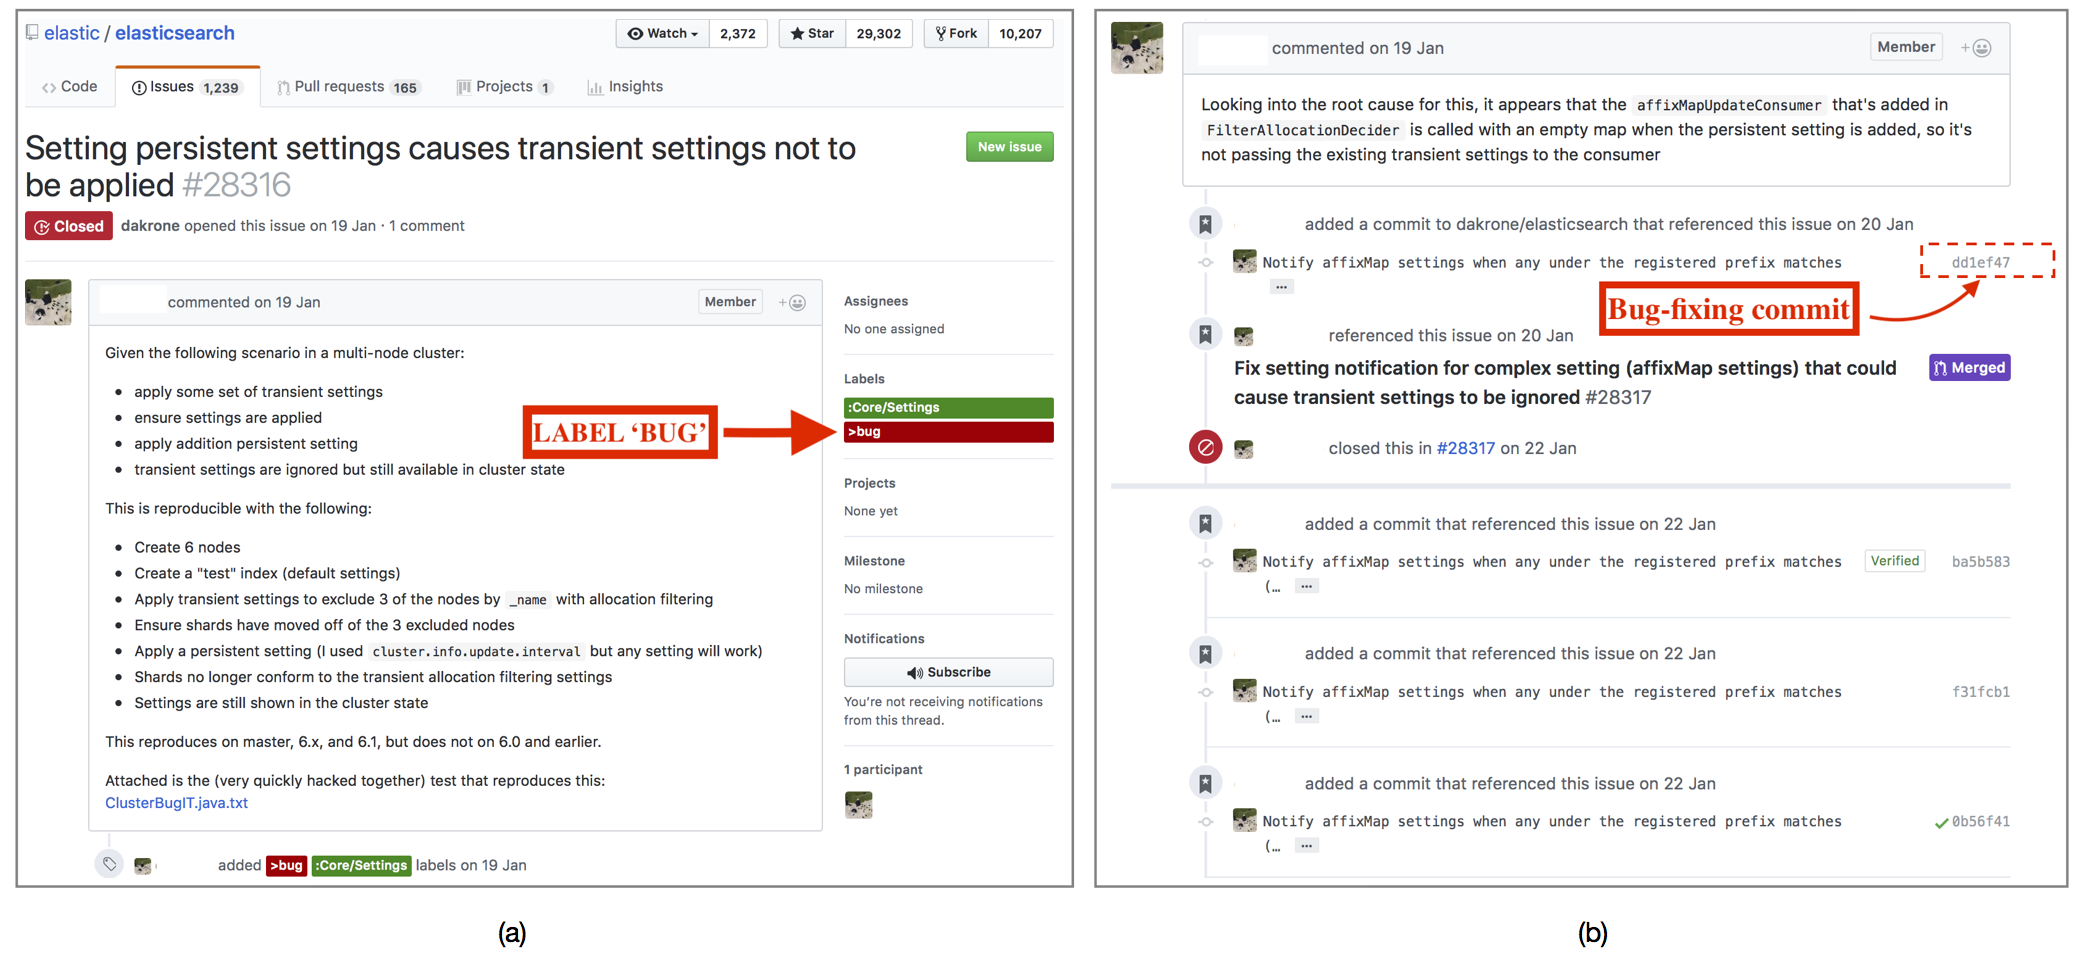
\includegraphics[width=\columnwidth]{img/bugreport.png}
\caption{Bug Report in ElasticSearch}
\label{fig:bugreport}       % Give a unique label
\end{figure}

The source code management systems also stores the source code and their differences across different versions of the source code, they store metadata such as user-IDs, timestamps, and commit comments. This metadata explains who, how, when, and why the source code is changed. Therefore by using this information and the information from the bug report, it is possible to understand which malfunction was caused by the bug, what problems in the source code were causing it, and how it was finally fixed.

Figure~\ref{fig:bugfix} \emph{(a)} shows the message of a commit that fixed the bug \emph{\#28316}, this information is accompanied by the diff of the files that have been modified to fix the bug in GitHub. Figure~\ref{fig:bugfix} \emph{(b)} shows the log entry of this bug-fixing commit from the git repository of ElasticSearch. This commit log information can be readily obtained using the command \emph{git show} and the number of the commit. Git's log entry includes the author, date, and files involved in the change. Additionally, a text message describing the change is also recorded. This message is the same as the message in GitHub. %\gema{Creo que deberiamos cambiar la figura, poner como se ve en github y como es la version en git normal}

\begin{figure}[ht]
\centering
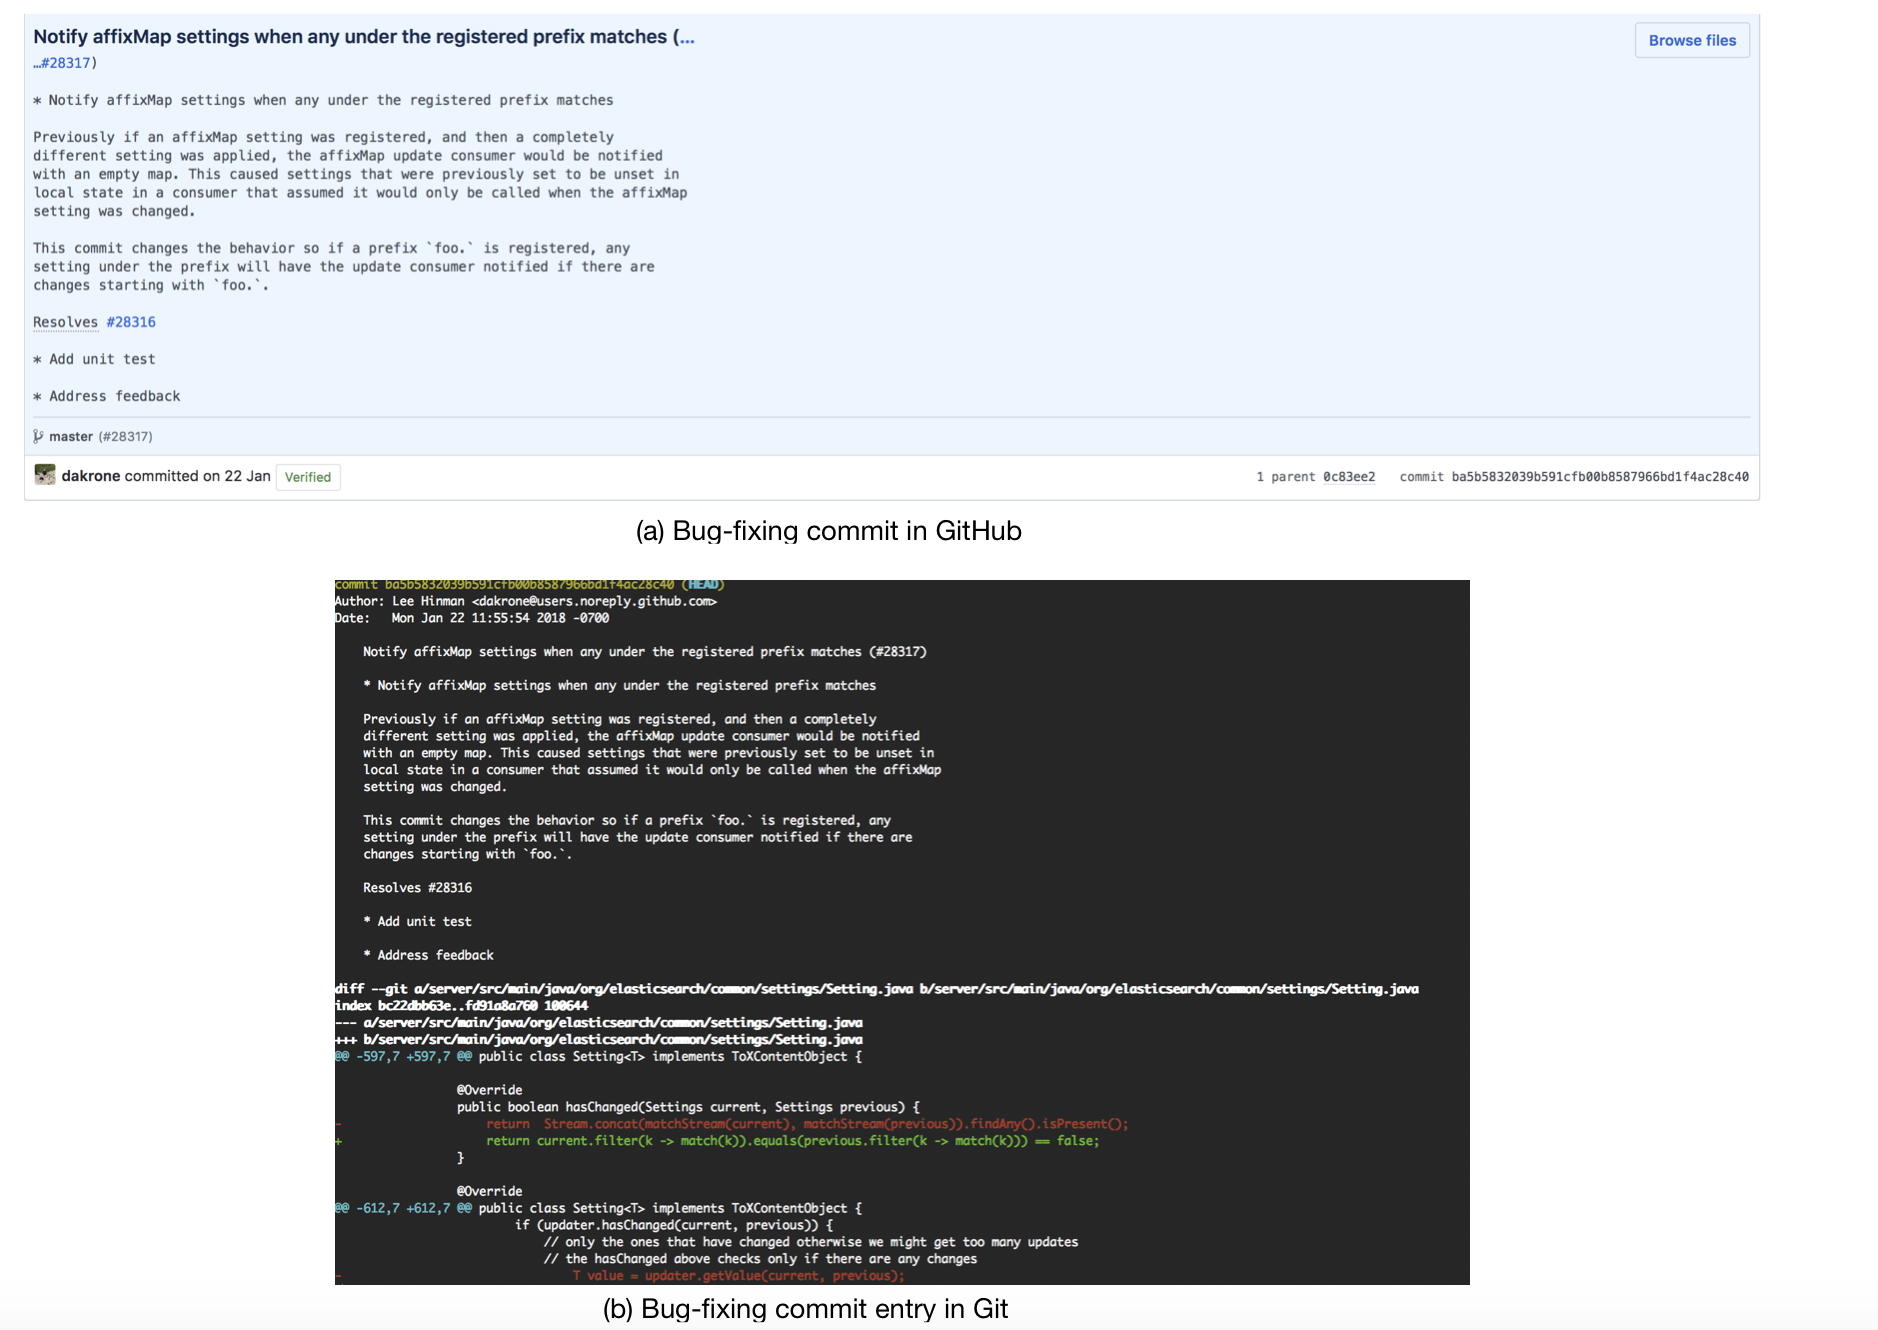
\includegraphics[width=\columnwidth]{img/bugfix.png}
\caption{Bug-Fixing commit in ElasticSearch}
\label{fig:bugfix}       % Give a unique label
\end{figure}

%Figure 1 shows a log entry from the Subversion repository of kdelibs (a part of KDE repository). A log entry corresponds to a single commit operation. This commit log information can be readily obtained by using the command–line client svn log and a number of APIs (e.g., pysvn). Subversion’s log entries include the dimensions author, date, and paths involved in a change-set. In this case, the changes in the files khtml_part.cpp and loader.h are committed together by the developer kling on the date/time 2005-07- 25T17:46:20.434104Z. The revision number 438663 is assigned to the entire change-set (and not to each file that is changed as is in the case with some version- control systems such as CVS). Additionally, a text message describing the change entered by the developer is also recorded. Note that the order in which the files appear in the log entry is not necessarily the order in which they were changed.

With all these data, the history of a software component can be navigated to identify when a malfunction was occurring for the first time. Using the \FFC, we might determine procedures to determine if given a bug reported and its corresponding fix and which change was the first one to manifest the malfunction.

%This way, we introduce the concept of ``first failing change" to extend the notion of ``introducing" (or ``seeding") a bu, as we commented before in the introduction. Using the \FFC, we might determine procedures to determine if given a bug reported and its corresponding fix, which change the first one to show a malfunction.

\subsection{SZZ algorithm}
\label{subsec:SZZintro}
%\gema{Brief discussion of the SZZ algorithm}

In Software Engineering research, the SZZ algorithm~\cite{sliwerski2005changes} is a popular algorithm for identifying the origin of a bug~\cite{da2016framework,rodriguez2018reproducibility}. It was proposed by \'Sliwersky, Zimmermann, and Zeller in 2005 to identify the suspicious change to induce the later fix. The algorithm identifies the bug-fixing commit, then uses a diff tool to compare the lines that differ between two revisions of the same file. In the SZZ, the authors assume that the lines that have been removed or modified in the bug-fixing commit are the ones containing the bug. For this reason, SZZ traces back the lines through the code history (by means of the annotate/blame\footnote{Annotate is used in SVN and blame is used in Git} command), to find when the changed code was introduced.

Even though the algorithm addresses two different problems, it can be split into two main parts. The first part is related to the problem of linking to the VCS and the issue tracking system to identify the bug-fixing commit. In this part, the algorithm identifies -by means of a set of heuristics- bug-fixing commits through employing a technique that matches commits with bug reports labeled as fixed in the bug tracking system. Therefore, the algorithm uses regular expressions to identify bug numbers and keywords in the commit messages that are likely to point out a real bug fixing change. %\gema{Write a little more about the first part}
The second part address the problem of identifying the bug-introducing commit. In this part, the algorithm employs the diff functionality implemented in the source code management systems to determine the lines that have been changed (to fix the bug) between the fixed version and its previous version. Then, using annotate/blame functionality, SZZ is able to locate who modified or deleted those lines for the last time in previous commit(s), and, whether they were committed before. Those change(s) are flagged as suspicious of being the bug-introducing commit(s).

After the publication of this approach, two main areas in software engineering \emph{(SE)} were improved and deeply studied. The first area clearly includes studies relate to the introduction of bugs~\cite{ pan2009toward,eyolfson2011time,asaduzzaman2012bug,bernardi2012developers,yangbug}. By studying bug-introducing commits identified using the SZZ algorithm, researchers are able to correlate some characteristics of the software evolution of the project with time, such as the day that a change is recorded with the introduction of bugs~\cite{sliwerski2005changes}, the time between when a bug was reported and the moment it was inserted~\cite{rodriguez2017much} or even if developers are fixing their own bugs~\cite{izquierdo2011developers}. The second area includes studies that attempt to avoid the introduction of changes in the future based on the study of prior bug-introducing commits. For example, avoiding bugs by using just-in-time (JIT) quality assurance practitioners and researchers build models that predict whether a change is likely to be a bug-introducing commit before committing it into the source code~\cite{kim2008classifying,kamei2013large,kamei2010revisiting,nagappan2006mining}.

Despite being a fundamental algorithm in the community to locate the bug-introducing commits, their results are limited. Firstly, there is not enough empirical evidence supporting the assumptions suggested by the SZZ, and the current evaluations are limited; Secondly, this algorithm \gema{does not work good in} some scenarios, i.e, when new lines in the bug-fixing commits cannot be traced back, these types of commits are removed from the analysis. Thirdly, despite there are some studies facing challenges with this algorithm~\cite{kim2006automatic,williams2008szz,da2016framework}, all of them have the same assumption: `` The lines changed to fix a bug are the ones containing the malfunction".

This thesis tries to shed some more light on how this algorithm performs in identifying the bug-introducing commit through empirical evidence. Furthermore, the reason why algorithms such as the SZZ are failing to identify correctly which change caused the failure is studied further.

%Despite the foundational role of SZZ, the current evalua- tions of SZZ-generated data (the indicated bug-introducing changes) are limited. When evaluating the results of SZZ implementations, prior work relies heavily on manual anal- ysis [9, 11, 26, 27]. Since it is infeasible to analyze all of the SZZ results by hand, prior studies select a small sample for analysis. While the prior manual analyses yield valuable insights, the domain experts (e.g., developers or testers) were not consulted. These experts can better judge if the bug-introducing changes that are identified by SZZ correspond to the true cause of the bugs.

%With respect to the bug fixing activity detection, the authors used the same approach as used in this dissertation: a commit is fixing an issue if this is identified as using the pattern: key word “bug” or “Bug” plus an id reference number.

\section{Research goals}
\label{subsec:goal}
\gema{Not reviewed}
% \gema{Poner los estudios donde la gente dice el dinero que pierde las empresas y esas como afecta a la productividad bla bla bla}.
Finding the root cause of bugs has been a hot topic during last years. The high importance and impact that this topic has is a key factor to understand and improve other areas related with bugs, such as to detect bugs, to prevent bugs or to analyze and compute statistics based on bugs in the projects. Thus, several questions have been raised to be considered in this dissertation, all of them are related to solve the problem of locating the change that caused the failure, as we demonstrate in Chapter~\ref{chap:Theory} all the bugs are not caused in the same way, and they do not present the same symptoms, thus they cannot be treated as equal when locating the origin of the bug.

\begin{figure}[ht]
\centering
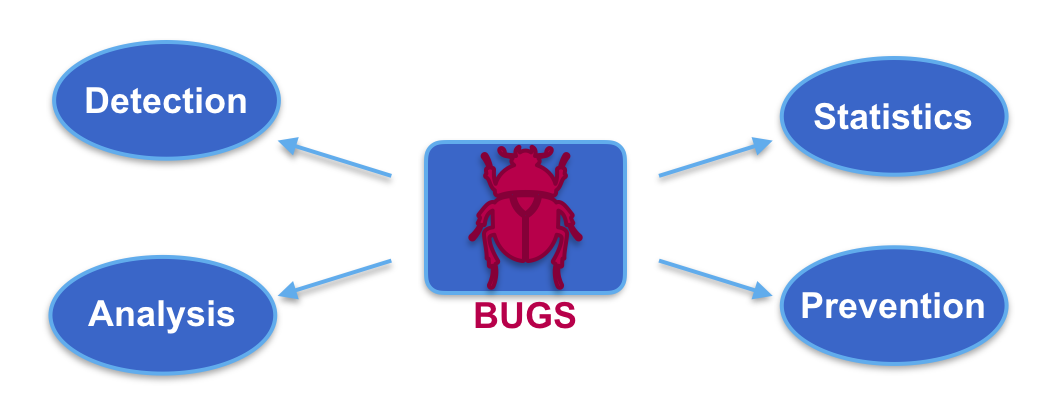
\includegraphics[width=\columnwidth]{img/SZZimportant.png}
\caption{SZZ}
\label{fig:SZZ}       % Give a unique label
\end{figure}

There are many studies and approaches based on track back the lines of a bug fixing commit to locate the origin of bugs. However, this approaches are not using any meaningful model that researchers can used to validate the algorithms used until now. In the sense that, these algorithms attempt to locate the ``original bug" or ``the root cause" or the ``origin of the bug", but researchers cannot be sure about what to introduce a bug means, because there is not any previous study that clearly defines the fact of introducing a bug and the moment of when it was introduced. Thus, they are not sure whether a bug introducing is the actual moment when the bug has been introduced. And, this is the reason why we are distinguish between bug manifestation moment (First-Failing Commit) and the bug introduction moment (BIC). Because, it is possible that we have a FFC without a BIC, for example because of external resources. That way, we have a moment when something has manifested itself but the reason is not related to the code, but it is related to a change in the environment.

To solve the lack of definitions and the need to validate the current algorithms. We propose a theoretical model to define how bugs are introduced that assuming we can have the perfect test and, this test can be run forever in the past, we can find out when the bug was introduced and whether this commit is responsible for the bug or it was something external. This model will work as a framework to validate the performance of other approaches. Furthermore, with this model, we can compare different algorithms to see how effective they are. Thus the main value of the thesis will be setting this framework because the previous literature does not address many cases and we need somehow to extend the model. But we cannot only set the framework, we also have to say where we can apply it.


\section{Contributions}
\label{subsec:contributions}
\gema{Not reviewed}
We outline the contributions of this thesis below. The contributions are grouped by their respective studies.

\paragraph{Study 1:}
We have carried out a study to analyze reproducibility and credibility in Empirica Software Engineering~\emph{ESE} with the SZZ algorithm as case of study. This study has been published in the Information and Software Technology Journal in March, 2018 \cite{rodriguez2018reproducibility}. The aim of the SLR is to obtain an overview of how authors have addressed the reproducibility and credibility in the studies where they have used the SZZ.

The contributions of this study are described below:
\begin{enumerate}
  \item \textbf{An overview on the impact that the SZZ has had so far in ESE:} The SZZ algorithm has been shown to be a key factor to locate when a change induced fixing-commits. Furthermore, to provide insight of how widespread the use of SZZ is, we also addresses the maturity and diversity of the publications where SZZ has been used in order to understand its audience.
  \item \textbf{An overview of how studies that use the SZZ algorithm address the reproducibility in their research work:} Reproducibility is a crucial aspect of a credible study in ESE~\cite{gonzalez2012reproducibility}. Piwowar et al. state that reproducibility improves the impact of research~\cite{piwowar2007sharing}. In addition, when a research work incorporates reproducibility, it is more likely to be replicated. However, there is evidence in the ESE literature that replicable studies are not common~\cite{robles2010replicating}. By providing a replication package, the authors facilitate others to replicate or to reproduce their experiment, which increases the credibility of their results~\cite{juristo2009using}.
  \item \textbf{An analysis of these studies manage the limitations of SZZ:} Limitations of SZZ are well-known in the research literature. we would like to find out how many papers report any of these. Therefore, we study whether authors mention the limitations of SZZ that may affect their findings, be it in the description of the method, in the threats to validity or in the discussion.
\end{enumerate}

\paragraph{Study 2:}
We have developed a comprehensive model of how bugs are introduced, including definitions and a taxonomy which help to analyze formally the process. The taxonomy helps to understand the many different ways in which a bug is introduced, and why some of the methods proposed in the literature fail to find many of them. The model allows as well for a better framing of the comparison of automatic methods to find bug inducting changes, which we apply to analyze some of these methods. Finally, based on this comparison, we propose some method that at least in the cases considered show better results than the classical methods described in the literature.

The contributions of this study are described below:
\begin{enumerate}
  \item \textbf{A detailed definition of the first failing change:} It introduces a general method to determine, unequivocally and falsifiability, the first time that the software fails in relation with the bug-fixing change.
  \item \textbf{The relation of the first failing change with its environment:} This relationship details the dependencies of a change in a specific moment, because it makes no sense to explain when a bug manifests itself by first time whether there is not explanation of the dependencies in which this bug appear.
  \item \textbf{A classification of the first failing change due to its nature}.
  \item \textbf{The rules to define the effectiveness of an algorithm when searching for the origin of the bug.}
\end{enumerate}

%\paragraph{Study 3:}
%\gema{Aqui me gustaria poner el estdudio sobre SZZ line based and token based }


\section{Structure}
\label{subsec:structure}
\gema{Not reviewed}
%\gema{Quiza escribir un poco mas sobre cada capitulo}
The remainder of this thesis is organized as follows. This chapter has depicted an overall idea of the main fields of study in this thesis. Specifically, focused on the bug seeding activity, describing the version control system and one of the most used algorithms for identifying the commit that introduce the bug.

In Chapter~\ref{chap:stateoftheart}, we provide a detailed description of the state of the art to the reader. First, we mention the studies in bug seeding and bug detection fields and we detail the bibliography related to the SZZ algorithm.

In Chapter~\ref{chap:context} we discuss the current problem to locate the moment when the system fails by first time by providing motivating examples and explaining the reasons why the current algorithms are inaccurate when locating the bug-introducing commits.

In Chapter~\ref{chap:credibility} we discuss the impact and how researchers use the SZZ in order to study the credibility of their results in the ESE.

In Chapter~\ref{chap:Theory} is the main body of this work and contains a detailed description of our proposed approach to deal with the innaccurate algorithms to locate the moment when the bug manifest the failure by first time. This approach can be modelated through the theory of bug introduction and this model allows as well for a better framing of the comparison of automatic methods to find bug inducting changes.

In Chapter~\ref{chap:application} we apply our proposed model into two cases of study: ElasticSearch an Nova, both are open source projects with many thousand of actives developers. We study how bugs were injected in the source code by manually navigating back into the lines of code that have been involved in the bug-fixing commit. Then we apply the theory of bug introduction to see how these projects behave when different methods are used to identify the origin of a bug. %the results from manual analysis to identify the exact location of the BIC in two different projects addresses the reasons why a previous commit may not induce the fix.

Finally, in Chapter~\ref{chap:conclusions}, we draw our conclusions and also discuss the results obtained with the threats to validity. Moreover, we also discussion about the approach followed and its potential applicability, and we conclude with the potential further work to be done.

%Moreover
%Pareto phenomenon
%Who should resolve the bugs?
% Someone who had similar bugs in the past!
%A bug you like: A framework for automated assignment of bugs
%Reducing the effort of bug report triage: Recommenders for development-oriented decisions
%Automatic bug triage using semi-supervised text classification
%An empirical study of the integration time of fixed issues

%Tangled commit also introduced more noise to locate the BIC, but with the FFC we do not concerned about them, because we these modifications are not in the 'test' that we want to pass to previous versions "The Impact of Tangled Code Changes (paper to read)" %%%%%%%%%%%%%%%%%%%%%%%%%%%%%%%%%%%%%%%%%%%%%%%%%%%%%%%%%%%%%%%%%%%%%%%%%%%%%%%%
%%%%%%%%%%%%%%%%%%%%%%%%%%%%%%%%%%%%%%%%%%%%%%%%%%%%%%%%%%%%%%%%%%%%%%%%%%%%%%%%
% BACKGROUND %
%%%%%%%%%%%%%%%%%%%%%%%%%%%%%%%%%%%%%%%%%%%%%%%%%%%%%%%%%%%%%%%%%%%%%%%%%%%%%%%%

\cleardoublepage
\chapter{State of the art}
\label{chap:stateoftheart}
In this chapter, the outline an overall picture of the bug life cycle, bug seeding and bug location process in the Software Engineering~\emph{(SE)}. The Bug seeding helps with identifying of root cause of bugs: It also helps in other areas of~\emph{SE} such as bug prediction, bug triage or software evolution. In this chapter, we describe the related work that is necessary to understand how this thesis fits into the current literature. The life cycle of a bug and the work that other authors have done to locate its origin its explained.

\section{Bug Life Cycle}
\label{subsec:buglife}
In this section the mian focus is on understanding a the bug's life cycle. Sommerville ~\cite{sommerville2010software} claims that it is not possible to avoid the unintentional introduction of bugs in the source code because it is inherited in the process os software making. To help with this process, several tools and product quality have been developed in order to reduce the number of bugs and improve the software development process.

Generally, the open source projects leave the management of issues to specific tools such as the Bug Tracking System. The open source systems studied in this dissertation uses Launchpad and Github as their Bug Tracking System, although the best-known bug tracking system is Bugzilla\footnote{ww.bugzilla.org/}. For example, in Bugzilla the life of a bug starts when a developer or user detects a wrong behavior and reports it to the system. The initial status of the report is UNCONFIRMED. Developers legitimatize the status by reproducing the symptoms described in the report where it is confirmed, meaning that the bug is real. The status is changed to NEW, and the bug is considered open from here onwards. An open bug's status is changed to ASSIGNED once it is assigned to a developer for fixing. The status of a bug changes to RESOLVED when its resolution is either: FIXED, DUPLICATE, WONT-FIX, WORKSFORME, INVALID, REMIND, LATER. Next, a Quality Assurance (QA) person might verifies the resolution by either accepting it or rejecting it, turning the outcome to either VERIFIED or REOPEN. Finally, when a bug is labeled as VERIFIED it can be marked as CLOSED which concludes the bug resolution process. Although the steps above describe the common process of a bug, there are other possible paths in the life cycle of a bug.

During this cycle, the developers and users might discuss about the possible cause of the bug or the reason why the project manifests the failure. Thus, the greater the understanding of a bug's life cycle, the greater the explanation of the root cause.

\subsection{Characteristics of bugs}

With this respect, previous works have studied bug characteristics in large software systems~\cite{chou2001empirical,gu2003characterization,ostrand1984collecting,ostrand2002distribution,podgurski2003automated, sullivan1992comparison,chen2014empirical,li2006have,beizer2003software,tan2014bug}. Recent papers  performed empirical studies to characterize and classify the bugs in open source software depending on the different challenges that arise in the bug finding process. Lu~\emph{et al,.} classified bugs in three categories depending on their root cause: Semantic, Concurrency, and Memory~\cite{lu2005bugbench}. Then, Li Tan~\emph{et al,.} extended the previous root cause classification by adding more cases, while also introducing two more dimensions, Impact and Software Component \cite{tan2014bug}. Table~\ref{tab:dimensions} shows how the root cause is related with the fault, the impact is related with the failure caused by the bug, and lastly, the component is related with the location of the bug~\cite{li2006have}. Finally, Chen~{et al.,} included additional sub-categories after manually studying how bugs  are introduced in a version of the software system, but they are not found until much later affects the quality of software systems ~\cite{chen2014empirical}. Assadollah~{et al.,} proposed a detailed classification of bugs depending of its root cause: memory related bugs, concurrent bugs and semantics bugs.


%many efforts have been made to generally define defect characteristics,(i.e., the IEEE Std. 1044 scheme \cite{isdw20101044}, and the Orthogonal Defect Classification (ODC) \cite{chillarege1996orthogonal}). The ODC classifies defects depending on several attributes such as the \emph{defect type} which is related to the semantic of the bug fixing commit, or the \emph{defect trigger} which is related to the verification and validation activities that cause the manifestation of the bug ~\cite{(Chillarege and Bassin, 1995; Chillarege and Prasad, 2002; Cotroneo et al., 2013d).}

%Recent papers performed empirical studies to characterise and classify the bugs in open source software depending the different challenges that the detection tools performs in finding bugs. Lu~\emph{et al,.} classified bugs in three categories depending on their root cause: Semantic, Concurrency, and Memory~\cite{lu2005bugbench}. Then, Li Tan~\emph{et al,.} extended the previous root cause classification by adding more cases, and they also introduce two more dimensions, Impact and Software Component. . Table~\ref{tab:dimensions} shows how the root cause is related with the fault, the impact is related with the failure caused by the bug, and finally, the component is related with the location of the bug~\cite{li2006have}. Finally, Chen~{et al.,} included additional sub-categories after manually study how bugs which are introduced in a version of the software system, but they are not found until much later affects the quality of software systems ~\cite{chen2014empirical}. Table~\ref{tab:rootcause} shows the final classification of bugs depending on its root cause: memory related bugs, concurrent bugs, semantics bugs.

\begin{table*}
\centering
\newcommand{\specialcell}[2][l]{%
  \begin{tabular}[#1]{@{}l@{}}#2\end{tabular}}
% increase table row spacing, adjust to taste
\renewcommand{\arraystretch}{1.3}
\caption{Bug categories of the three dimensions: Root Cause, Impact, and Component}
\label{tab:dimensions}

\begin{tabular}{lll}
\toprule
\textbf{Dimension}& \textbf{Subcategory}& \textbf{Description} \\
\midrule
\multirow{3}{*}{Root Cause}&Memory & Improper handling of memory objects. \\
&Concurrency & Synchronization problems\\
& Semantic & \specialcell{Inconsistencies with requirements or \\programmers' intention}\\
 \hline
 \multirow{6}{*}{Impact}& Hang & Program keeps running but does not respond.\\
    & Crash&Program halts abnormally.\\
    & Data Corruption&Mistakenly change user data.\\
    & Perfor. Degradation& Functions correctly but runs/responds slowly.\\
    & Incorrect functionality&Not behaving as expected.\\
    &Other&other impacts.\\
 \hline
 \multirow{4}{*}{Software Component}& Core& Related to core functionality implementations.\\
 &GUI &  Related to graphical user inter- faces.\\
 &Network&Related to network environment and communication.\\ 
 &I/O& Related to I/O handling.\\
 \bottomrule
\end{tabular}
\end{table*}


\begin{table*}
\centering
\newcommand{\specialcell}[2][l]{%
  \begin{tabular}[#1]{@{}l@{}}#2\end{tabular}}
% increase table row spacing, adjust to taste
\renewcommand{\arraystretch}{1.3}
\caption{Categories of root causes of bugs found in \cite{asadollah2015towards,chen2014empirical,lu2005bugbench}}
\label{tab:rootcause}

\begin{tabular}{lll}
\toprule
\textbf{Category}& \textbf{Subcategory} & \textbf{Description} \\
\midrule
\multirow{7}{*}{Concurrency}&Data race&Two or more threats access to write the same data\\
&Atomicity-related& A concurrent overlapping execution between two sequences\\
& Deadlock & A process depend by another process to proceed\\
& Order Violation&Violation of the desired order\\
& Livelock& A thread is waiting for an unavailable resource\\
& Starvation& A process idefinitely delayed \\
&Suspension&A calling thread waits for a long time\\
 \hline
 \multirow{6}{*}{Memory}& NULL Pointer Dereference & Dereference of a null pointer\\
   %& NULL pointer exception  \\
    & Memory leak &Failures to release unused memory \\
    &Uninitialised Memory Read & Read memory data before it is initialized\\
    &Dangling Pointer & Pointers still keep freed memory addresses\\
    &Overflow & Illegal access beyond the buffer boundary\\
    &Double Free & One memory location is freed twice\\
 \hline
 \multirow{10}{*}{Semantic}& Missing Cases&A case in a functionality that is not implemented\\
 &Missing Features&A feature that is not implemented\\
 &Corner cases&Incorrect or ignored boundary cases\\ 
 &Wrong control flow&Incorrect implementation of sequences of function calls\\
 &Exception handling & Do not have proper exception handling\\
 &Processing &Incorrect Evaluation of expressions/equations \\
 &Typo & Typographical mistakes \\
 &Design Issue & Incorrect Design or API/function\\
 &Incorrect Documentation & \specialcell{Incorrect/inconsistent documentation of \\software and source code}\\
 &Other & Any other semantic bug\\
\bottomrule
\end{tabular}
\end{table*}

Many authors have used this classification to deal with different purposes regarding automatic approaches for software bug classification, as well as empirical and methodological studies on the case of software errors, taxonomic studies for software bugs and the study of bug characteristics in the OSS. Vahabzadeh~\emph{et al,.} attempts to understand the characteristics of bugs in test code. In this study the authors also insert  the \emph{Environment} category when referring to tests that pass or fail depending on the operating system and the incompatibilities between different versions of JDK. They discovered that incorrect and missing assertions are the main root cause of dormant bugs\cite{vahabzadeh2015empirical}. Jeffrey~\emph{et al,.} developed a technique to automatically isolate the root cause of memory-related bugs; their approach is effective in finding root causes when memory corruption propagates during execution until a failure crash occurs\cite{jeffrey2008identifying}. Wan~\emph{et al,.} studied 1,108 bug reports in order to understand the nature of the bug, they also introduced other categories such as \emph{Security}, \emph{Environment and Configuration}, \emph{Build}, \emph{Compatibility} and \emph{Hard Fork}. Their findings indicate that security bugs take the longest median time to be fixed, and also that the environment and configuration bugs are one of the major types of bugs along with the semantic bugs \cite{wan2017bug}. \gema{quiza hablar un poco mas de este estudio}\gema{anadi andy works abou enviromental CI ms paper 2017}

On the other hand, some authors have also considered using other characteristics to classify bugs. Sahoo~\emph{et al,.} used the reproducibility of a bug, the observed symptoms and the number of inputs needed to trigger the symptom to distinguish between deterministic, time dependent or non-deterministic bugs \cite{sahoo2010empirical}. Chandra and Chen distinguished environment-dependent  from environment-independent bugs in the Apache, GNOME, and MySQL \cite{chandra2000whither}. Zhang~\emph{et al,.} computed the bug fixing time and identified factors that influence it on three open source software applications. They found the assigned severity, the bug description, and the number of methods and changes in the code as impacting factors.

%More papers to read
%Albert Endres. An analysis of errors and their causes in system programs. ACM SIGPLAN Notices,
% Victor R. Basili and Barry T. Perricone. Software errors and complexity: an empirical investigation.
% Mark Sullivan and Ram Chillarege. A comparison of software defects in database management systems and operating systems. 


\section{Bug Seeding and Bug Location}
\label{subsec:bugSeedingBG}

To locate the origin of bugs, researchers have proposed two different procedures. Some researchers use techniques starting with a bug-fixing commit in order to identify the most recent commit(s) that was changed to fix the bug. Other researchers use techniques to locate root causes of software failures by analyzing program traces. These approaches do not rely on identifying the bug-fixing commit, instead they attempt to find an association between program failures and the execution of program elements.

In this section, the state of the art processes for identifying the bug-fixing commits as well as bug-introducing commits are discussed. Although this thesis is mainly motivated in the techniques that uses the bug-fixing commit to identify the commit that caused the bug, other existing and popular techniques are also discussed.

\subsection{Identifying the bug-fixing commit}

Previous works have attempted to identify bug-fixing commits in version archives. Mockus and Votta performed an analysis to identify the reasons for software changes using historic databases; they used the textual description in the log of a commit to understand why the change was performed~\cite{mockus2000identifying}. Cubrani\'c and Murphy recommended a practice that uses a bug report number in the comment when the practitioners fix a bug report, thereby linking the changes with the bugs~\cite{vcubranic2003hipikat}. Finally, \'Sliwersky~\emph{et al.} proposed the~\emph{SZZ} algorithm that links a version archive to a bug database in order to automatically identify and analyze fix-inducing changes~\cite{sliwerski2005changes}; the authors made use of the previous work mentioned before, and also benefited from Fischer's~\emph{et al.} work in which they proposed a technique to identify references to bug databases in log messages, then used these references to infer links from VCS archives to BUGZILLA databases~\cite{fischer2003analyzing,fischer2003populating}. In summary, the SZZ automatically links change logs and bug reports using some heuristics which search for specific keywords (such a `` Fixed" or ``Bug") and bug IDs (such a ``\#1234") in change logs \cite{bachmann2009software,mockus2000identifying,schroter2006if,zimmermann2007predicting}. This heuristic relies on `` developers leaving hints or links regarding bug fixes in the change logs"\cite{wu2011relink} . 

However, the quality of the change logs are not ensured as they may incorrectly link with the bug-fixing commit from the version archives with issue reports that are not bug reports from the issue tracking system. Bird~\emph{et al.} discovered that the absence of bug references in change logs affected the number of missing links leading to biased defect information, thereby affecting defect prediction performance \cite{bird2009fair}. Researchers have further investigated this misclassification during the past years as the heuristics might yield biased data, Bird and Bachmann et al. confirmed this problem and reported that 54\% of bug reports are not linked to bug-fixing commits \cite{bachmann2010missing,bird2009fair}. Bettenburg~\emph{et al.}  noticed that the issue reports often present incomplete and incorrect information \cite{bettenburg2008makes}. Antoniol~\emph{et al.} noticed that many of the issues in issues tracking systems did not describe bug reports \cite{antoniol2008bug}. Herzig~\emph{et al.} found that around one third of the bug reports that they manually analyzed were not describing a bug \cite{herzig2013s}. Nguyen~\emph{et al.} showed that even in a near-ideal dataset, the biases exists \cite{nguyen2010case}.

On the other hand, some researchers have attempted to mitigate the limitations and shortcomings of linking bug reports with bug fixing commits \cite{herzig2013s,rodriguez2016bugtracking,tan2015online}. Thus,  practice, tools and algorithms have been developed in order to mitigate this problem. For instance, GitHub supports linkage by automatically closing issues whether the commit message contains the \emph{\#numberOfIssue}, many Free/Open Source Software projects have adopted as a good practice to use keywords in their commit comments such as ``\# fix-bug -" when they are fixing a bug, as it has been reported for the Apache HTTP web server7 in \cite{bachmann2010missing}, and for VTK8, and ITK9 in \cite{mcintosh2016empirical}. In addition, several authors have suggested the used of semantic heuristics \cite{schroter2006if,vcubranic2003hipikat,zimmermann2007predicting} , while others have proposed solutions that rely on feature extraction from bugs and issue tracking system metadata. For Instance, Wu~\emph{et al.} developed ReLink to automatically link bugs reports and commits based on the similarity between the texts in both \cite{wu2011relink}. Bird~\emph{et al.} suggested manual inspections by developers in order to identify missing links. They proposed the tool LINKSTER that helps developer to locate possible links by providing query interfaces to the data \cite{bird2010linkster}. Nguyen~\emph{et al.} proposed the Mlink tool to mitigate some of the problems found in ReLink, for instance some code changes in the commit are excluded and both issue reports and commit are used as plain texts \cite{nguyen2012multi}. Le~\emph{et al.} continued working on the shortcomings of the previous tools and develop RCLinker, which enriches commit logs. This approach extracts textual and metadata features from issues and commits \cite{le2015rclinker}. As a consequence of these efforts, the linkage problem has been addressed and its accuracy has drastically increased. For example, FRlink, an existing state-of-the-art bug linking approach, has improved the performance of missing link recovery compared to existing approaches, and it outperforms the previous one by 40.75\% (in F-Measure) when achieving the highest recall \cite{sun2017frlink}.

\subsection{Identifying the bug-introducing commit}

Failure-inducing\footnote{Notice that some authors use failure-inducing as the concept for bug-introducing} changes were first addressed by Ness and Ngo in 1997~\cite{ness1997regression}. They described how to identify a single failure-inducing change using simple linear and binary search. Their goal lies in isolating failure-inducing changes by applying chronological changes to a program until the fixed version presents the same wrong behavior as the next version of the program. Despite this, the technique is able to reduced the computational cost of testing each combination of changes introduced in the faulty version to locate the failure-inducing changes. However, this technique fails when instead of one change, a set of changes cause the failure. To deal with the issue, Zeller proposed the automated delta debugging technique, which can determine the minimal set of failure-inducing changes by gradually increasing granularity to identify the differences (that is, the deltas) between a passing and a failing subset~\cite{zeller1999yesterday}.

Purushothaman and Perry~\emph{et al.} measured the likelihood for small changes, particularly one-line changes, to introduce errors. They refer to fix-inducing changes as~\emph{dependencies} which are changes to lines of code that were changed by an earlier commit. They assume that if the latter change was a bug fix, the original change was erroneous. The study concludes that the probability of a one-line causing a bug to be less than 4\%~\cite{purushothaman2004towards}. Baker and Eick also used a similar concept when referring to fix-inducing changes,\emph{fix-on-fix changes}. However, this concept requires both changes to be fixes. The paper describes a graphical technique for displaying large volumes of software where directories and subdirectories with high fix-on-fix rates were identified~\cite{baker1994visualizing}.

\paragraph{When a bug-fixing commit exists:}

As previously mentioned,\'Sliwersky~\emph{et al.} proposed by first time an algorithm, the SZZ, that locates fix-inducing changes in version archives~\cite{sliwerski2005changes}. Although the SZZ algorithm provides a technique to identify possible bug-introducing changes, it has to deal with the incorrect identification of bug-inducing changes. For this reason, many efforts have been made to suggest improvements to the SZZ algorithm. First, Kim~\textit{et al.} developed an algorithm that automatically identifies bug-introducing changes; the algorithm is based on improvements of the SZZ algorithm that remove false positives and negatives by using the \textit{annotation graph} technique instead of using VCS \textit{annotate} to locate the lines changed in the bug-fixes. With this modification, the SZZ may avoid some false positives by not considering 
non-semantic source code changes, (i.e. blank spaces, changes in the format or changes in the comments) and by ignoring outlier fixes. After a manual validation, the new version of SZZ can remove about 38\%-51\% of false positives and 14\%-15\% of false negatives~\cite{kim2006automatic}. Secondly, Williams and Spacco proposed another enhancement of the SZZ algorithm. The authors suggested to use a mapping algorithm instead of the annotation graphs because they are more precise when facing larger blocks of modified code in bug fixes; this new approach uses weights to map the evolution of a unique source line and ignores comments and formatting changes in the source code with the help of \texttt{DiffJ}, a Java-specific tool. The authors also verified how often the bug-introducing changes were the true source of a bug in a small sample size, where 33 of 43 lines mapped to a bug fix showed evidence of a bug being introducted~\cite{williams2008szz}. Then, Da Costa~\textit{et al.} realized that during the last ten years there was not much research conducted to evaluate the results of the SZZ, they proposed a framework that evaluates the results of the different SZZ implementations based on a set of criteria such as the earliest bug appearance, the future impact of changes, and the realism of bug introduction. Their findings suggest that the previous SZZ enhancements tend to inflate the number of incorrectly identified bug-introducing changes, and by using this framework, the practitioners can evaluate the data generated by a given SZZ implementation and they might eliminate unlikely bug-introducing changes from their outcome~\cite{da2016framework}. Campos Neto~\textit{et al.} worked on improving the SZZ algorithm by disregarding refactoring changes as the bug-introducing changes because they do not change the system behavior. The authors empirically investigated the impact of such refactoring in both changes, bug-fixing and bug-introducing. Their results indicate that their approach can reduce 20.8\% of the incorrect bug-introducing changes when compared to the first SZZ approach \cite{neto2018impact}.

Other authors have created new approaches based on the same concept as SZZ algorithm, by attempting to mitigate the incorrect identification of bug-introducing changes. Kawrykow and Robillard developed \emph{DiffCat}, a tool-supported technique to detect and remove non-essential changes in the revision histories of projects. Their findings showed that up to 15.5\% of system's method updates consisted entirely of non-essential modifications, \cite{kawrykow2011non}. Ferdian~\textit{et al.} looked at the root cause of the bugs by applying a combination of machine learning and code analysis techniques, then verifying their approach through comparing the results with their manual analysis of 200 bug reports. This approach identifies the erroneous lines of code that cause a chain of erroneous behavior in the program leading to the failure; it has a precision of 76.42\%, and a recall of 71.88\% \cite{thung2013automatic}. Servant and Jones introduced the fuzzy history graph; this technique helps to represent the code lineage as a continuous metric providing a balance of precision and recall. This technique performs better over the evolution of the code when compared to other models \cite{servant2017fuzzy}.  

Other techniques are related to dependence techniques. These approaches also attempt to locate the bug-introducing commit; they address some of the shortcomings in the text-based approaches by examining the behavior of the changes by using a program dependence graph (PDG). Dependence-based techniques compare the PDG for the bug-fixing change to the PDG for the previous version. First, PDG only identifies removed dependencies, it only examines added dependences when no dependences were removed and returns only the most recent version involved. Sinha~\textit{et al.} introduced this technique in order to identify the bug-introducing commit by analyzing the effects of bug-fixing commit on program dependences. This is a significant improvement over the text approach used by the SZZ algorithm, as this approach takes into account semantics of code changes, similar to previous work \cite{horwitz1990identifying, binkley1992using}. This make the approach to be more accurate and applicable to a wider class of bug-fixing changes (i.e., changes that involve addition of statements). Their results increased the precision and the recall of the fixes by 19\% and 15\% when compared to the text approach~\cite{sinha2010buginnings}.  After this technique was introduced, many additions and refinements were made. Davies ~\textit{et al.} compared text-based and dependence-based techniques for identifying bug origins. The authors suggested detailed improvements to identify bug origins by combining both techniques \cite{davies2014comparing}. 

\paragraph{When a bug-fixing commit do not exist:}

Contrary to the previous authors, some authors have studied the origin of bugs  without identifying the bug-fixing commit;  and they have developed different methods such as Delta Debugging \cite{misherghi2006hdd,zeller2002simplifying,cleve2005locating,zeller2002isolating}, Spectrum Based Fault Location \cite{reps,janssen2009zoltar,harrold2000empirical,tiwari2011spectrum,abreu2007accuracy,jones2002visualization}, Nearest Neighbor \cite{renieres2003fault,jones2002visualization,abreu2007accuracy}, set union and set intersection \cite{}.A brief description of each method is given as follows. 

\emph{Delta Debugging} Zeller and Hildebrandt described the Delta Debugging algorithm for the first time in ~\cite{zeller2002simplifying}. This algorithm compares the program states of a failing and passing run, while using binary search with iterative runs. The iterations stop when the smallest state change that caused the original failure is identified.  In other words, this technique defines a method to automatize the process of making different hypotheses about how changes affect output to locate failure causes.  Gupta~\textit{et al.} used Delta Debugging combined with dynamic slicing to identify the set of statements that is likely to contain a faulty code~\cite{gupta2005locating}. Cleve and Zeller~\cite{cleve2005locating} presented the Cause Transitions technique and compared it to the Nearest-Neighbour technique. Their results suggest that, on the same set of subjects, Cause Transitions technique performs better than Nearest Neighbour.

\emph{Spectrum Based Fault Location}: A method used to locate faults from the identification of the statements involved in failures was first introduced in~\cite{reps}. This technique usually takes as inputs two sets of spectra, one for successful executions and the other for failed executions. It reports candidate locations where causes of program failures occur (e.g., lines, blocks, methods, etc.), which may be presented to debuggers. There are many spectra such as node spectra, edge-pair spectra, edge spectra and block spectra. Jones~\textit{et al.} developed the Tarantula system which provides a way to rank statements in terms of their likelihood of being faulty. Furthermore, it has a graphical user interface that specifies a color for each statement in the program depending on the suspiciousness of being buggy\cite{jones2002visualization}. Abreu~\textit{et al.} investigate the diagnostic accuracy of the spectrum-based fault localization as a function of several parameters using the Siemens Set benchmark. Their results indicate that the superior performance of a particular coefficient is largely independent on test case design~\cite{abreu2007accuracy}.

%( Lightweight defect localization for Java.) AMPLE (Analyzing Method Patterns to Locate Errors) [5] is a system for identifying faulty classes in object- oriented software. It collects hit spectra of method call sequences, which are subsequences of a given length that occur in a full trace of incoming or outgoing method calls, received or issued by individual objects of a class. Each call sequence is assigned a weight, which captures the extent to which its occurrence or absence correlates with the detec- tion of an error, i.e., it is a combined measure of similarity and inverted similarity. These weights are averaged over all call sequences of a class, leading to a class weight. Classes with a high weight are most likely to contain the fault that causes the detected error. 

\emph{Nearest Neighbour}. Renieres and Reiss used Nearest Neighbour queries to locate the fault~\cite{renieres2003fault}. This technique contrasts a failed test with a successful test which in terms of distance, is more similar to the failed test. It uses these two test cases to remove the set of statements executed by the passed test case from ones executed by the failed test case. A bug is then located whether it is in the difference set between the failed run, and its most similar successful run. In case the bug is not contained in the difference set, this technique continues constructing a program dependence graph, while adding and checking adjacent un-checked nodes in the graph until the bug is located. This method is easily applicable since it only requires a classification of the runs as either incorrect or faulty from the users.

\emph{Set union and Set intersection}
The set union computes the union of all statements executed by passing test cases and taking these from the set of statements executed by a failing test case. The suspicious statements are contained in the resulting subset of all coverage entities that the user must explore. While this is happening, the set intersection computes
the set difference between the set of statements that are executed by every passed test case and the set of statements that are executed by a single failing test case. A set of statements is obtained by intersecting the set of statements executed by all passed test cases and removing the set of statements executed by the failed test case. \gema{rephrase it} 


%- Micro interaction metrics (MIMs) that leverage developers' interaction information (Micro Interaction Metrics for Defect Prediction)

\paragraph{Tools for locating bugs:}

A lot of effort have been made to develop practical tools that assist in locating and detecting the bugs. Without trying to be exhaustive, a brief description of some tools that have been used to find bugs in the source code is given.

FindBugs\footnote{http://findbugs.sourceforge.net} is an automatic detector for bugs with the same pattern in Java source code.  The user experience of this tool showed that it was helpful and most of the warnings fixed in a specific organization were ``hashcode/equals problems, serialization issues, unchecked method return values, unused fields and constants, mutable static data, and null pointer dereferences" \cite{hovemeyer2004finding}. HATARI is a plugin for Eclipse that determines how risky is a change depending on the area of source code\cite{sliwerski2005hatari}.   PMD\footnote{http://pmd.sourceforge.net/snapshot/} tool is a static code analyzer that checks the source code of a project in order to find possible bugs, dead code, suboptimal code or overcomplicated expressions. It checks for patterns in the abstract syntax tree of parsed sources files \cite{copeland2005pmd}. Jlint\footnote{http://jlint.sourceforge.net/} is a tool that checks for bugs, inconsistencies and synchronisation problems in Java code \cite{artho2001finding}.FixCache has a similar purpose, files and methods are saved and maintained in the cache; when a bug is fixed, these elements are updated and the cause of the bug is identified. The cache can be used to predict how likely a change in an area might cause another bug \cite{kim2007predicting}. BugMem identifies project-specific bugs and suggest corresponding fixes, it uses a learning process of bug patterns of project-specific bugs \cite{kim2006memories}.  OpenJML\footnote{http://jmlspecs.sourceforge.net/} is a compile-time checker tool that warns against potential runtime errors and inconsistencies between the design decision recorded and the actual code. It is the successor of ESC/Java. The feedback of users using this tool supports that it can detect real software defects \cite{flanagan2013pldi}. BugLocalizer\footnote{https://github.com/SoftwareEngineeringToolDemos/FSE-2014-BugLocalizer} is implemented as a Bugzilla extension, and it uses information retrieval (IR) based bug localization that computes similarities of the bug report with source code files with the aim of locating the buggy files~\cite{thung2014buglocalizer}. Commit Guru\footnote{http://commit.guru} is a tool that identifies and predicts suspicious buggy commits. The tool also provides downloadable analytics to users on the likelihood of a recent commit to introduce a bug in the future, the percentage of posible commits that may have introduced buggy code in their projects, etc. \cite{rosen2015commit}. 

%Similarly to previous studies [Kim et al., 2008, S' liwerski et al., 2005], this research is performed at the granularity level of source lines, which provides a way of handling the ambiguity of working with commits. When considering the committer A who fixes a certain bug, and the lines she modifies, some of these lines could have been introduced fully or partially by the same committer, or introduced by different committers without the participation of A (pictured in Figure 1). Extending these two basic scenarios, we could find further scenarios:
%1)the same set of lines was modified in a previous commit by the same developer A (only);
%2)the same set of lines was modified in a previous commit by a different developer B (only);
%3)the same set of lines was modified by more than one developer (A+B+C+...), including the same developer A fixing the bug;
%4)the same set of lines was modified by more than one developer (B+C+D+...), but excluding the developer fixing the bug;


%In terms of relating the bug-fixing process and its responsibilities, some authors have dealt with the idea of who should be fixing a certain bug [Kagdi et al., 2008, Ma et al., 2009] based on previous changes of the same file, or at least slices of the changes introduced in a file. Another approach used to deal with the same problem has been adopted at the level of the bug tracking system. In a study based on the development of Microsoft Windows Vista and Windows 7, it has been found that the number of reports "opened" by one developer and initially "assigned" to her development team tend to be fixed more quickly than bugs that are assigned to another development team [Guo et al., 2010].Finally, other authors have dealt with the idea of looking for bug-fixing patterns in the source code [Pan et al., 2009] analyzing the different revisions provided by a given SCM system, but focusing on the semantics of the source code. In other words, they are aware of several common fix patterns such as "addition of precondition check" or "different method call to a class instance". However, at the level of the source code, and to the best of our knowledge, no studies aiming to determine if developers that fixed the bug are the same than those who introduced the bug have been undertaken.

%\paragraph{Dealing with very large commits:} As reported in previous studies, software systems, and most noticeably FLOSS systems, display at times high (and isolated) peaks of activity. In some specific cases, it has been possible to detect a very large amount of source lines (e.g., more of 80\% of the overall system) being moved within FLOSS projects [Canfora et al., Hindle et al., 2008]. This means that in some changes, one can detect huge changes reaching million of lines. From a maintenance or evolutionary point of view, this is hardly accountable as a maintenance activity. However, this problem has not been taken into account by [Kim et al., 2008], whose analysis is one of the pillars for this study.

%Also in the study of the comm-central repository, it has been found that a small number of commits (no more than 10\% of the total set) handles several thousands (in some cases hundreds of thousands) of lines in just one commit. Apart from exceptional cases where developers indeed modified a vast amount of source lines, the peaks could also be caused by automatic bots, changes in the licenses, or by accidental removal and addition of source code. As an example of such distortions, figure 3 shows the number of aggregated number of removed lines4. The figure depicts a situation of common removal of lines, but in some specific commits, we can see how suddenly a large set of lines is removed (for example, close to id 723 or 4,200).
%In order to deal with such distortions, the commits fully or partially affected by those changes were removed from the sample: given an overall number of 2912866 lines and 2969 commits detected in the bug-fixing process, the sample was therefore reduced to 731941 lines and 1747 commits. In summary, the four largest commits (IDs 0; 1002; 817; 5213 and 53835), and the lines affected, were removed from the sample.
\gema{esto no esta editado}
\subsection{Testing}
Software testing is conducted in order to provide information about the quality of the software or service under test~\cite{kaner2006exploratory}. The test techniques include the process of executing an application with the purpose of finding software bugs before the software product is released.

Much work on software testing seeks to ensure the minimum human intervention by automatizing as much as possible the process, to make testing faster cheaper and more reliable. This work can be seen in the following categories:

%The currently software testing focuses on:
\textbf{Automatic software repair}, which is challenging because of its difficulty and, it is focus on two main fields, behavioral repair and state repair. Behavioral repair address the issue of test-suite based repair that states `` given a program and its test suite with at least one failing test case, create a patch that makes the whole test suite passing"~\cite{monperrus2014critical} and which has been explored by the Genprog. Genprog is a seminal and archetypal test-suite based repair system developed at the University of Virginia~\cite{weimer2009automatically,forrest2009genetic} whose evaluation in in a later study claims that 55 out of 105 bugs can be fixed by Genprog~\cite{le2012systematic}. Currently, people is still working on improving the core repair operators. On the other hand, the large research field of state repair address the issue of \emph{recovery} that focuses on ``a system state that contains one or more errors and (possibly) faults into a state without detected errors~\cite{laprie1985dependable}.

\textbf{Emulation of software faults} is used to evaluate fault tolerance procedures, and to assess the impact that a bug will have in the system. Dur\~aes~\emph{et al.} created a new fault injection technique (G-SWFIT) after observing that a large percentage of faults can be characterized with high accuracy, and that allows to use a small set of emulation operators instead emulate the software faults with a big set. allowing accurate emulation of software faults through a small set of emulation operators~\cite{duraes2006emulation}.\gema{quizas anadir un poco mas de esta categoria o eliminarla ....}


\textbf{Fault localization methods} based on the spectrum-based fault localization~\cite{abreu2009practical,jones2002visualization,jones2005empirical,liu2006statistical} help practitioners to locate faults by checking a small portion of source code. This techniques usually compute and rank the fault suspiciousness of single elements of a program by contrasting the program spectra information between passed and failed executions. Jones \emph{et al.} developed the \emph{tarantula tool} which is a visualization technique that uses color to visually map the results of executing a program with an entire test suite in which each program statement passes or fails, allowing to developers inspect the statements in the program and identify potential buggy statements~\cite{jones2002visualization}. And then, they present the first empirical study that compares a set of four existing automatic fault localization techniques with tarantula, in which tarantula pinpoint the fault three times more often than the best technique in the set~\cite{jones2005empirical}.


Nevertheless, when researchers use software testing to locate faults, they are not looking for the origins of the faults by understanding their reasons and their dependencies that may cause the problem that a clean line can become to be buggy. They usually are focus on minimize the cost that a fault may cause in the system by guiding developers to the faulty location, and they do not try to rebuild the complete history of the system in each moment to know what was happening in that moment. Thus, to our knowledge, it is the first time that a paper presents an idea in which the software testing can be used to find the first time that a bug manifests itself in the software by locating the origin of the bug.\gema{poner algo sobre git bistec??}


\section{Studies on Bug Seeding:}
\label{subsec:SZZuse}

The foundational role of locating a bug origin in Software Engineering resides in its transversality. Once the origin of a bug is located, many different areas in Software Engineering can benefit from the knowledge. They can deliver different studies with different outcomes where practitioners can better learn practices to continue improving the current state of the art about bug seeding and software engineering. Without attempting to be exhaustive in the description, we offer several examples where authors have analyzed the origins of bugs with different general purposes. Five different categories were selected based on the origin of a bug performing an important role: bug prediction, bug location, bug classification, bug fix and software evolution.

\paragraph{Bug prediction:} Bug prediction is aimed at supporting developers to identify whether a change will be buggy or not. This area studies bug seeding and bug fixing activity as a potential source of prediction for further issues. For instance, Feng~\textit{et al.} collected the defect data and attempted to build a universal defect prediction model for a large set of projects from various contexts~\cite{zhang2014towards}. Jiang~\textit{et al.} proposed a novel technique that produces a personalized model for each developer; this model is used to predict bugs on future data~\cite{jiang2013personalized}. Hata~\textit{et al.} developed a fine-grained version control system for Java in order to conduct fine-grained prediction~\cite{hata2012bug}. Kim~\textit{et al.} analyzed the version history of 7 projects to predict the most fault prone entities and files; they identified the bug-introducing changes at the file and entity level~\cite{kim2007predicting}. Zimmermann~\emph{et al.} predicted bugs in large software systems such as Eclipse~\cite{zimmermann2007predicting}. Nagapan \emph{et al.} associated metrics with post-release defects to build a regression model that predicts the likelihood of post-release defects for new entities~\cite{nagappan2006mining}. Yang~\textit{et al.} studied what kind of bug-introducing changes are likely to become a great threat after being marked as bug-fixing changes~\cite{yang2014bug}. Rosen~\textit{et al.} developed a prediction tool base that identifies and predicts risky software commits~\cite{rosen2015commit}. Kamei \emph{et al.} used just-in-time \emph{(JIT)} quality assurance concept to build a model that predicts whether a change is likely to be a bug-introducing~\cite{kamei2013large}. Fukushima \emph{et al.} empirically evaluated the performance of defect prediction models based on Just-In-Time cross-project~\cite{fukushima2014empirical}.

%Copiado de buginnings
%There exists an extensive body of research on predicting the fault-proneness of code components. These techniques use the history of bug fixes made to a code component as one of the indicators of fault-proneness of the component (e.g., [4, 10, 19, 22]). Mockus and Weiss [18] proposed the use of change properties, such as size, diffusion, and change type (bug fix or new feature), as predictors of faults. Their approach computes these properties for those past changes that led to subsequent failures, and builds a predictive model to estimate the likelihood that a new change many have introduced faults. For the subject, the scenario, and the modification-tracking system that they studied, the iden- tification of maintenance requests that subsequently led to failures could be performed easily. However, in general, link- ing code changes to subsequent bug fixes is not a trivial task; an automated technique for accurately identifying bug- introducing changes is essential for a wider and practical use of change properties as indicators of fault-proneness.

\paragraph{Bug Classification:} Bug classification is aimed at supporting developers in classifying wthether a change is buggy or not. For example, Pan~\textit{et al.} described a program slicing metrics to classify changes as buggy or bug-free. They use SZZ to mark files that have bug-introducing changes~\cite{pan2006bug}. Kim~\textit{et al.} showed how to classify file changes as buggy or clean using change information features and source code terms~\cite{kim2008classifying}. Thomas~\textit{et al.} introduced a framework for combining multiple classifier configurations that improves the performance of the best classifier~\cite{thomas2013impact}. Ferzund~\textit{et al.} presented a technique to classify software changes as buggy or buggy-free based on hunk metrics~\cite{ferzund2009software}. Kim and Ernst proposed a history-based warning prioritization algorithm that helps to improve the prioritization of bug-finding tools~\cite{kim2007warnings}. Nguyen and Fabio Massacci conducted an empirical study to validate the reliability of the NVD vulnerable version data~\cite{nguyen2013reliability}.

\paragraph{Bug Location:} Bug location is aimed at supporting developers in identifying where a bug resides.
Asaduzzaman~\emph{et al.} applied the SZZ algorithm on Android to identify the changes that introduced the bugs, they then used this information to look for problems during the maintenance upkeep of the project~\cite{asaduzzaman2012bug}. Schr{\"o}ter~\emph{et al.} built a data set that contains the mapping between the bug reports and their bug-introducing commits in the Eclipse project~\cite{schroter2006if}. Kim~\emph{et al.} developed a tool to find bugs using the bug fix memories, which also focused on the knowledge of changes that fix bugs. The tool uses statistical-analysis to learn project-specific bug patterns by analyzing the history of the project and then suggest corrections~\cite{kim2006memories}. Wen~\textit{et al.} proposed the use of LOCUS, an IR-based bug localization tool based on the analysis of software changes and contextual clues for bug-fixing. The performance of LOCUS at source file level have  significantly improved, on average around 20.1\% and 20.5\%, as demonstrated in the results of MAP and MRR techniques \cite{wen2016locus}. Youm~\textit{et al.} developed BLIA, a statically integrated analysis tool of IR-based bug localization that uses information from bug reports, source files and source code changes histories. The authors claimed that this tool achieves better results than BugLocator, BLUiR, BRTracer and AmaLgam \cite{youm2015bug}.

\paragraph{Bug Fix:} Bug fix is aimed at supporting developers in improving the bug fixing process.
Researchers have studied who should fix a certain bug report~\cite{kagdi2008can,anvik2006should} based on previous changes of the same file. Another approach used by Guo \emph{et al.,} predicts whether a bug report will be fixed. This approach is based on the study of different characteristics and factors that affect the fix of bug reports in Windows Vista and Windows 7. This study found that bugs were more likely fixed when they were reported by people with higher reputation, or when they were handled by people on the same team \cite{guo2010characterizing}. Cincarini and Sillitti extended the previous study in an open source environment and confirmed the results found by Guo \emph{et al.,} \cite{ciancarini2016model}. Other authors have dealt with assigning bug reports to individual developers, Baysal \emph{et al.,} developed an approach that uses developer's expertise, current workload and preferences to assign the appropriate developer to fix a bug \cite{baysal2009bug}. Another common practice during the bug fixing process is to compute the time required to fix a bug after it was introduced into the source code. Kim and Whitehead computed the time to fix a bug in files of ArgoUML and PostgresSQL project. Their results indicated that the median was about 200 days~\cite{kim2006long}. Zang \emph{et al.} developed a Markov-based method for predicting how many bugs will be fixed in the future and the time required to fix them \cite{zhang2013predicting}. Some authors have conducted empirical studies to understand the usefulness of social platforms such as Twitter in the bug fixing process \cite{el2017tweets}. Finally, other authors, have studied the bug fixing patterns by using the SCM systems, they focused on the semantics of the source code \cite{pan2009toward}.

\paragraph{Software Evolution:} Software evolution is aimed at supporting developers in understanding how a software evolves and which characteristics (authorship, time of commit, developers' interaction ...) or patterns are implicated in the bug proneness.
Kim and Whitehead computed the time to fix a bug after it was introduced into the source code in ArgoUML and PostgresSQL~\cite{kim2006long}. Kim~\textit{et al.} also studied the properties and evolution patterns of signature changes in seven software systems written in C, using SZZ to identify the bug-introducing changes~\cite{kim2006properties}. Eyolfson studied whether the time of the day and developer experience affects the probability of a commit to introduce a bug~\cite{kamei2010revisiting}. Izquierdo~\textit{et al.} researched whether developers fixed their own bugs~\cite{izquierdo2011developers}; they also studied the relationships between experience and the bug introduction ratio using the Mozilla community as case of study~\cite{izquierdo2012more}. Rahman and Devanbu attempted to understand some factors that have a big impact on software quality such as ownership, experience, organizational structure, and geographic distribution~\cite{rahman2011ownership}. Posnett~\textit{et al.} studied the effect of artifact ownership and developer focus on software quality. They discovered that more focused developers introduce fewer defects than defocused developers~\cite{posnett2013dual}.  Bavota~\textit{et al.,} carried out an empirical study in three Java systems to investigate the extent of refactoring activities in introducing a bug \cite{bavota2012does}. 


%Herzig\textit{et al.} demonstrated that 33.8\% of all bug reports are misclassified and that 39\% of files marked as defective actually never had a bug~\cite{herzig2013s}.
%Reducing the effort of bug report triage: Recommenders for development-oriented decisions
%Automatic bug triage using semi-supervised text classification

%%%%%%%%%%%%%%%%%%%%%%%%%%%%%%%%%%%%%%%%%%%%%%%%%%%%%%%%%%%%%%%%%%%%%%%%%%%%%%%%
%%%%%%%%%%%%%%%%%%%%%%%%%%%%%%%%%%%%%%%%%%%%%%%%%%%%%%%%%%%%%%%%%%%%%%%%%%%%%%%%
% CONTEXT OF THE PROBLEM %
%%%%%%%%%%%%%%%%%%%%%%%%%%%%%%%%%%%%%%%%%%%%%%%%%%%%%%%%%%%%%%%%%%%%%%%%%%%%%%%%

\cleardoublepage
\chapter{Context of the problem}
\label{chap:context}

This chapter attempts to explain in detail the whole context of the current problem with identifying the precise moment when a bug was inserted into the source code of a software system. It then describes the many reasons why the current state-of-art approaches are not successful in correctly identifying bug-introducing changes. Finally, this chapter gives motivating examples to demonstrate the necessity for practitioners and researchers to search for another more accurate method for identifying of the moment when a bug is inserted into the source code.

In the previous chapters of this thesis we have described the important role of correctly identifying bug-introduction changes. There are many reasons for the explanation of this special interest. From the economic point of view, software bugs are costly to fix~\cite{lerner1994software} and they are highly time-consuming~\cite{latoza2006maintaining}. In 2009, the US National Institute of Standards and Technology (NIST) estimated that the US economy earmarks \$59.5 billion annually to fix software defects and to reinstall systems that have been infected. It is calculated that software developers use approximately 80\% of the total 59.5 billion to identify and correct defects~\cite{zhivich2009real}. From the research point of view, the knowledge of where the bug has been introduced by first time has important implications in software engineering disciplines as we have explained in~\ref{chap:Introduction}. However, specific characteristics of software evolution and maintenance complicate the correct identification process of the bug-introducting changes. For example, the complexity: software systems and their architecture are continuously evolving and becoming more complicated over time; this may lead to problems  that creeps into the system and manifesting as bugs~\cite{le2016architectural}. It may also lead to the manifestation of failures in unchanged parts~\cite{german2009change}.  The dependency of the source code with external artifacts: the component-oriented development model leads to the development of software products that are an assemblage of small components from many different sources. In this scenario, it will be tedious to estimate the behavior of the whole system when one of its components behaves erroneously~\cite{duraes2006emulation}; Lastly, the accuracy: The current approaches rely heavily on manual analysis to evaluate the results with the restriction that only the experts can judge if the changes identified using such methods are the real causes of the bugs. Unfortunately, this analysis will be impractical in most of the cases and there is not existing framework to correctly evaluate the results obtained after using different approaches to locate the bug-introduction moment~\cite{da2016framework}.

Thus, without a clear methodology to know exactly what line created a bug, many studies in the area of software maintenance and evolution start with the implicit assumption that the line (or lines) that is being replaced in a bug fix is likely the cause for introducing the bug. This assumption can be frequently found in the research literature, for instance in:

\begin{itemize}
  \item ``We assume that the last change before the fixing change was the change that introduced the defect''~[SLR\cite{cao2015investigating}].
  \item ``A fix-inducing is a change that later gets undone by a fix"~[SLR\cite{shippey2015exploiting}].
  \item ``The SZZ observes each hunk in the bug-fix and assumes that the deleted or modified lines are the cause''~[SLR\cite{shivaji2013efficient}].
  \item ``The defect was caused in one of the artifacts that was later edited to correct the defect''~[SLR\cite{vanhilst2011process}]. 
  \item ``The lines that have been removed of modified in the bug-fixing commit are the ones where the bug was located''~[SLR\cite{izquierdo2011developers}]
  \item ``We assume that the person who injected defects into a file is the person who changed it''~[SLR\cite{ando2015does}].
  \item ``We assume that faults are reported just after they are injected in the software''~[SLR\cite{yamada2014text}].
  \item ``To trace backwards through the version history to identify for each of these lines the last commit that has changed the line''~[SLR\cite{prechelt2014software}].
  \item ``[The] [b]lame feature of Git is used to identify the file revision where the last change to that line occurred''~[SLR\cite{bavota2015four}].
  \item ``We determine the defect-inducing change as the change that is closest and before''~[SLR\cite{wehaibi2016examining}].
  \item ``A line that is deleted or changed by a bug-fixing change is a faulty line''~[SLR\cite{tan2015online}].
  \item ``We mark those hunks as bug introducing in which we find the source code involved''~[SLR\cite{ferzund2009software}].
\end{itemize}

One of the key problems with the approaches when identifying the \BIC is the assumption that ``the modified line in a bug fixing commit is likely the one that introduced the bug". Although this assumption may appear reasonable at first glance given its frequent presence in research literature, there is not enough empirical evidence supporting it. Furthermore, recent studies have demonstrated the many limitations of this assumption~\cite{da2016framework, rodriguez2018reproducibility} when flagging potential changes as Bug-Introducing Commit. However, in a previous research work \cite{rodriguez2018reproducibility}, it was discovered that even when the researchers were aware of using this assumption and knowing full well of its limitations, they still use it in their studies. For example, some research have commented on the threat when a fixing commit only adds new lines, or when the line has been modified several times since its introduction, or when some lines that fix the bug are not related with it:

\begin{itemize}
  \item ``It is possible that previously in the history of the inspected line a large addition of lines has introduced this error, thus confusing the history of the line."~\cite{williams2008szz}.
  \item ``There are some bugs introduced in one place, but fixed in another place"~\cite{yuan2013predicting}.
  \item ``Fix locations may inflate the warning false positive rate. Additionally, adding new code may fix an existing warning"~\cite{kim2007warnings}.
  \item ``The SZZ algorithm used to identify bug-introducing changes has limitations: it cannot find bug introducing changes for bug fixes that only involve addition of source code. It also cannot identify bug-introducing changes caused by a change made to a file different from the one being analyzed."~\cite{shivaji2013reducing}.
  \item ``It is extremely hard to automatically understand the root of vulnerabilities."~\cite{nguyen2013reliability}.
  \item ``In a fix of a crash-related bug, not all of the changes are aimed to address defects. Some lines may be added because of a refactoring or an addition of a new feature. These changes are hard to identify with an automatic approach."~\cite{jongyindee2011good}.
  \item ``Additionally, it is not necessary that a bug may have been introduced in the most recent CVS transaction that changed the relevant lines in the file."~\cite{abreu2009developer}.
\end{itemize}

However, researchers cannot be sure whether a bug-introducing change is the actual moment when a bug is been introduced, as the term bug is undefined, thereby making it impossible to understand what it means to introduce a bug. When the approaches place blame on a line that contains the bug, this line should not be isolated from the context of when it was inserted by first time. This is because based on this context, researchers can understand whether the line that introduced the bug occurred at that particular moment, or rather on the contrary, the line was correct in that moment of time but defected later due to changes in other parts of the code causing it to manifest in that specific line. For example, when a source code is using a third-party code, and it changes something in the API without a previous notification, it could be possible that at some point the lines of the source code  manifests a bug. This however does not mean that the lines of the source are responsible for inserting the bug, as they could be perfectly clean when it was first written into the source code. As such, in this example, the bug has not been introduced in the lines, the bug has been caused by the evolution of a third-party code.

The main problem lies in the current literature and  how we act of introducing a bug is defined as well as how the moment of its introduction is defined. It is possible that both moments are the same, but it is also equally possible that they are different. The latter case has not been addressed in the actual state-of-the-art literature. Thus, the current heuristics and approaches need to be extended;  there is the necessity to build a model that contemplates all the different scenarios in order to re-define the theory of bug introduction. Fortunately, in modern software development many traces can be retrieved on how code changes, and how bugs are fixed. Thanks to that, many information are at disposal where when analyzed, provides the means to understand the reasons why a change was required to fix a bug. Thus, before building a model, we can use information from the source code management system, the issue tracking system and the code review system to first understand the malfunction that instigated change, then identify what problems in the source code were causing it, and finally how it was fixed.

%Empowered with all these data, we navigate back in the history of the software component, to find out when the malfunction manifested itself for the first time. This way, we introduce the concept of ``first failing change'' (\FFC) to extend the notion of ``introducing'' (or ``seeding'') a bug. Without a clear definition of what is the bug, a developer can hardly say when it was inserted, specially, when she keeps in mind that likely the bug had been caused by a change unrelated with the code she is fixing~\cite{german2009change}. For this reason, the concept of \FFC makes easiest to understand that there exists a moment in which the software manifested the malfunction and theoretically, we would find such moment only navigating back in the history of changes. Therefore, we will use the concept of \FFC to define procedures and determine if a given change was the first one to show the malfunction. From there, we will show how there are cases when the first failing change is not the change introducing the bug, in the sense that the change was not caused by a developer, and for that reason it does not make sense try to find the bug introduction change when analyzing why the code is behaving erroneously. Furthermore, we will also use this concept to compare the effectiveness of different methods for the identification of bug introducing changes.

\section{Effectiveness of Current Approaches in Finding the Bug-Introducing Commit}
 
From a general point of view, until now, approaches based on tracking back the lines of a bug fixing commit are not using any meaningful model that researchers or practitioners can employ to validate the algorithms. The lack of definition on what should be validated makes it difficult for researchers to describe what a false positive, true positive, false negative and true negative is. These algorithms attempt to find which commit inserted the ``seed" of the bug, but there is no differentiation between which which commits inserted the bug and which commit did not inserted the bug. The current algorithms also do not distinguish between the moment of introduction and the moment of manifestation. For these reasons, researchers cannot be sure about what it means to introduce a bug. To measure the recall and precision of their approaches, many of the researchers use the concepts of false/true positives and false/true negatives without taking into account the real meaning of these concepts. Nowadays, the approaches compute the precision and the recall using the following definitions:

\begin{itemize}
  \item \emph{True positive} : Given a commit identified by one of the approaches after applying the heuristics to the modified lines in a Bug-Fixing Commit,  a true positive is when the latest commit that modified the line, inserts a bug into the source code; the bug is fixed when the line that is modified by the latest commit is fixed. This definition of true positive means that the commit is likely to be the cause of a bug, but researchers cannot be sure whether or not it inserted the bug into the system. 
  \item \emph{False positive}: Given a commit identified by one of the approaches after applying the heuristics to the modified lines in a Bug-Fixing Commit, a false positive is when the commit that last modified the lines in a source code did not insert a bug, but the algorithm flags it as a bug introducing commit.. For example, if the commit inserted blank lines that changed the format of a function by moving a bracket or adding a tabulation, added or modified comment lines, or when a variable in the source code is renamed. This definition of false positive implies that the commit is not the cause of a bug. 
  \item \emph{False negative}: Researchers have different perceptions of what a false negative is; Da Costa \emph{et al.} defined it as ``a bug-introducing change that is not flagged as such by SZZ"~\cite{da2016framework}. Kim \emph{et al.} assumed that their improved version of SZZ is more accurate than the original, and computed the false negatives as ($ |K-S|/K $), where \emph{``K"} is the set of bug-introducing commit detected by their algorithm, and \emph{``S"} as the set of bug-introducing commit detected by
SZZ~\cite{kim2006automatic}. Davies \emph{et al.} defined it as ``commits that introduced bugs but which are not identified by the approaches"~\cite{davies2014comparing}. Surprisingly they did not find any false negative in their study. 
  \item \emph{True negative} : Any commits that was not identified by the approaches and is not responsible for introducing the bug.
\end{itemize}

However, as mentioned earlier, these definitions of true and false positive are not completely correct, because they are not based on understanding whether or not the identified lines inserted the bug at the time of their writing. . Thus it is imperative to establish proper definitions for, the concepts regarding false positive, false negative, true positive and true negative, as can be seen below:

\begin{itemize}
  \item \emph{True positive} \gema{reprhase}: Given a commit identified by one of the approaches after applying the heuristics to the modified or added lines in a Bug-Fixing Commit, a true positive is when this commit modified the source code of a project inserting a bug in the lines at that moment. 
  \item \emph{False positive} \gema{reprhase} Given a commit identified by one of the approaches after applying the heuristics to the modified or added lines in a Bug-Fixing Commit, a false positive is when this commit modified the source code of a project but it did not insert a bug in the lines, because at that moment the lines were clean. Some examples or false positives are described through the next paragraphs of  this section.
  is when a line identified by an algorithm is not the line that introduced the bug because in the moment of its insertion that line was clean. \gema{False positive: Given a commit identified by one of the approaches after applying heuristics to the modified or added lines in a Bug-Fixing Commit, a false positive is when the commit modifies the source code of a project but did not insert a bug into the lines. This means that in the moment, the lines were still clean. Some examples of false positives are described in the following parts of this section. False positives are when a line identified by an algorithm is not the line that introduced the bug because in the moment of its insertion the line was clean.}
   \item \emph{False negative} \gema{reprhase} is when a commit cannot be identified by the algorithms, and it introduced a bug in some of the line(s) modified or added at the moment of writing.
  \item \emph{True negative} is when a commit cannot be identified by the algorithms and it did not introduce the bug at the moment of committing the changes.
\end{itemize}

Nevertheless, the approaches built on back tracking the lines of a bug fixing commit searches for the last commit that touched the line(s) that was modified to fix a bug, the \emph{previous commit(s)}. After applying this approaches to a bug fixing commit, there is a set of previous commits that can contain only one or more than one different previous commits. Thus, researchers have to decide which previous commit from the previous commit set is causing the bug. It however can be possible that the bug-introducing commit is one or none of the previous commit. It can be none because a bug could have been either introduced in new lines in other parts of the code, or a bug has been introduced by an external artefact or because the environment has changed.

The reasons why the current approaches in some cases are not able to identify the BIC are the following: \gema{maybe a figure in each scenario?}

\paragraph {Identification of more than one previous commit:} A bug-fixing commit may have more than one line edited (deleted, modified or added), and in cases where a developer changed more than one line to fix a bug, it is possible that the previous commit of these lines were different. Thus, when the approaches to find the suspicious bug-introducing commit are applied, there may be different previous commits to blame for the cause of the bug. The main problem in this case is that the current state-of-the-art approaches do not provide any guidelines on how practitioners or researchers should behave in these situations. Moreover, the researchers in the articles do not explain clearly the heuristics that they have used in the instance that the scenarios come up. This might be a big source of false positives.

\paragraph {When only new lines are used to fix the bug:} There are some bugs that are fixed by simply adding new lines to the source code. This may occur when some ancestor commit forgets to add lines to the source code. As a result, when the system fails, the developers need to fix the bug by adding new lines to the source code. For example, a commit may forget to add a null-pointer dereference. The fix adds a null-check line, while the lines of the commit that have forgotten to add the code are not changed. However, the current approaches removed these cases from their analysis because the new lines cannot be tracked back. As a consequence, these approaches are not able to identify the bug-introducing commit which causes the presence of false negatives in these scenarios.

\paragraph {Changes in the environment or configuration:} There are some bugs that manifest itself before a change in the environment or during the configuration. These kinds of defects correspond to the bugs that lie in third-party libraries, underlying operating systems, or non-code parts (e.g. configuration files). Thus, when one of the part changes without any previous notification to the developers, the system experiments with the failure, and the developers are required to change the lines that are affected by the ecosystem or the configuration of the project to fix the project. The issue here is that when the current approaches are applied, the previous commits are identified as the bug-introducing commit when in fact, they did not introduce the bug. This is because when the lines are inserted by first time, they were initially correct for the ecosystem at that point in the time. In these cases, the approaches are introducing false positives.

\paragraph {Multiple modifications of a line:} The evolution of the source code of a project affects the identification of bug-introducing changes due to the necessity for the implementation of new requirements. When the source code of a new requirement is committed, the code might alter the identity of the previous commit in a line. For instance, when the commit \emph{123aa} is inserted into the function \emph{func}, and later the commit \emph{456bb} inserts a new functionality into the project that modifies the function \emph{func} by adding a new argument to it. In these cases, the last commit that touched the line of the function \emph{func} is the commit \emph{456bb}, and it may recur for a long time in a line. The problem lies in whether the commit \emph{123aa} was responsible for inserting the bug. In this case scenario, the current approaches cannot identify it, while pushing the blame to the false positives commits as the Bug-Introduction Commits, because they were the last commits that modified the line that is failing.

\paragraph {Weak semantic level:}  A key factor in the correct identification of bug-introducing changes is the comprehension of the changes made in each commit. The modifications of lines are addressed for different purposes; some modifications are made to optimize the code while the same behavior remains in the code, other modifications are made to rename variables or functions or to remove dead code, while other modifications simply copy and paste lines from other commits. All of these modifications are semantic, which causes the approaches to identify false positives bug-introducing commit. On the one hand, the false positive may occur because the real change that introduced the buggy behavior to the source code was before the modifications, and that the semantic changes are hinting towards the real cause. On the other hand, the false positive may occur because the approaches might identify numerous, suspicious commits, when in fact they are simply semantic changes and should instead be removed from the analysis.

\paragraph {A bug fixing commit that fixed more than one bug:} Although it is not common for a bug-fixing commit to fix more than one bug, sometimes due to the close relationship between the bugs or the dependency between them, researchers can find that a bug-fixing commit closed more than one bug report. This causes the approaches used to identify the Bug-Introducing Commit to identify false positive commits even though the two bugs addressed in the same bug-fixing commit have been introduced in different commits. 

\paragraph {Compatibility:} These kinds of cases correspond to the bugs that make a system fail or pass depending on the particular CPU architecture, operating system, or Web browser used. For example, user \emph{A} never experimented a bug when using the project under macOS, but user \emph{B} who is using Windows had experimented the bug due to the failure of the project using this OS. Thus, with these kind of bugs it will not be faire to lie the blame on a previous change or an ancestor change as the bug-introducing commit, because the developers' intentions and the circumstances of the moment cannot be known for certain whether it will later fail when they submit the source code. In these cases, the current approaches also identify false positives bug-introducing commits.

\paragraph {Dormant bugs:} Tse-Hsun \emph{et al.} have investigated in depth this type of bugs. The characteristics of the bugs is that when they are introduced in an earlier version of the system, they are not reported until much later. Thus, when the current approaches are applied to the bugs to find the bug-introducing commit, the result are false positive. Sometimes, lines fixed in the bug-fixing commit are not responsible for introducing the bug. This could be due to the natural evolution of the source code where other developers may have modified some parts of the dormant buggy code. The approaches identified as a result identifies the modifications as the bug-introducing change.

It is clear that the effectiveness of the current approaches is not up to standard for practitioners and researchers. This problem lies mainly on how these approaches work. The approaches identifies the chronologically last modification of a fixed line as the bug-introducing version, but it is now apparent in may scenarios that these approaches fail because of this reason. This thesis explores a new concept of the first failing commit, based on the hypothetic idea that there is a perfect test and it can be run forever in the past. Let's take \emph{Vn} as a version and \emph{t} as the perfect test with a coverture of 100\%. A fault can be revealed given a fixed version \emph{Vn+1}. Assuming that \emph{t} is an oracle that tests how the behavior of the fixed lines should be in \emph{Vn} and previous versions of \emph{Vn}, it is possible to identify the buggy version regardless of  whether the test fails. For instance, as the test knows what the bug is and what should be the correct behavior of the source code at that point, if the test passes, it means that this version did not introduce the bug, and it continues to backtrack the version history of the source code. The approach starts with the version \emph{Vn-1}, where it executes the test in each version to identify the version that fails. This version will be the First-Failing Commit and also the Bug-Introducing Commit depending on other factors. More details are found in Chapter \ref{chap:Theory}.


%Si el error no se ha introducido en ningún commit de los PC set, se ha podido introducir perfectamente en uno de los anteriores. O en la combinación de varios de ellos, con lo cual, lo que nosotros hacemos en realidad es seguir un poco hacia atrás. Y ahí viene, el problema de cuando lo ves desde ese punto de vista definir como se introdujo ese cambio. Esto es algo donde tenemos que hacer incidencia puesto que hay muy poca literatura sobre esto, (buscar lo poquito que hay : condiciones). Si no hay una definición clara de que es el error, es muy difícil decir cuando se introdujo el error, sobre todo si tienes en cuenta que el problema se ha podido causar por algo que ni siquiera está en el árbol de cambios anteriores. Es entonces cuando nosotros llegamos a la idea de si ahora pintamos el árbol (git blame) de una forma temporal, hay un momento temporalmente en el que el error se empieza a manifestar y ese seria el momento donde se introdujo el error. ---> Esto es conveniente introducirlo desde un punto de vista abstracto, sin hablar de test todavía, si no que como hay que definirlo y precisamente lo que se busca es cuando se introdujo el error, pues habrá un momento en el que las distintas versiones del programa, una de esas versiones experimenta  el fallo, fallo que se
%está corrigiendo en el FC. Y para eso es conveniente aplanar el árbol git blame, porque vemos que a partir de un FC todos los arreglos tienen una historia, incluso si hay otros cambios. Lo que pasa que al mapear los commits del árbol en su version aplanada, el orden cronológico puede cambiar debido a que si hay rebase y merges el más a la izquierda no necesariamente significa que es el más antiguo en tiempo, pero si desde el punto de vista de reconstrucción de la historia. Y la cuestión es que cuando encuentres el cambio que introdujo el error, las versiones siguientes también manifiestan dicho error. --> Comentar una ejemplo donde no se suceda el orden cronológico entre commits del git log y citar el articulo de daniel sobre perils and pitfalls de git.

%Lo importante no es cuando (en tiempo) se introdujo si no qué commit lo introdujo (historia). A partir de que un cambio lo introdujo en cualquier parte del árbol, el error está introducido en el programa, por que ya cualquier cambio tiene el error. --> Preguntar ejemplos a Daniel sobre casos de merge o rebase de linux. Todo esto para explicar que en git la relación temporal no es relevante y que ademas tenemos dos fechas, la del autor que es cuando se creo el código y la del commit que depende de cuando se metió.




%“What is a bug-introducing code version” may be subject to different interpretations. It is possible that a bug fix modifies parts of a program that were previously touched in different versions. In such a case, should a tool identify the chronologically last version, the chronologically first version, or all versions as bug-introducing?

%Moreover, the type of analysis performed determines the extent to which multiple versions are computed. Consider a bug fix that modifies many semantically related state- ments. An approach, such as the text approach, that does not consider the relations among the statements would check for each modified statement, where the statement was last touched. If the statements were touched in different ver- sions, the approach would return multiple versions. In con- trast, an approach that considers the relations among the statements would return the version in which the relations were created.




\section{Motivating examples:}
In this section we present real motivating examples found in the project that was analyzed. These examples clearly describe the necessity to distinguish the difference between the Bug-Introduction moment and the First-Failing Commit. There are different kind of bugs, some of them were directly introduced but others have manifested themselves in the system without the necessity of being introduced. Thus, the nature of bugs provide a guide to find other approaches to identify the first change that manifested the malfunction, enabling the understanding of whether the change also introduced the bug. The next examples support this urgent necessity by explaining what caused the bug when the bug manifests and how other approaches fail to identify the bug-introducing commit. It is important to keep in mind that the logic of the most famous approaches to identify bug introducing changes is through looking at the previous changes that touched the fixed lines in the bug-fixing commit. In case there are more than one change, these approaches use heuristics to determine which lines contain the fix that caused the bug. It may be one, or a combination of many . It could also be none of the previous changes or none of the ancestral changes. In fact, the bug cannot be caused by any previous commit or any ancestor commit because the bug was caused by a change in an external artifact that the project uses.

%Ejemplo de los subdirectorios
The first example is the bug \#3820\footnote{https://github.com/elastic/elasticsearch/issues/3820} from ElasticSearch. Figure~\ref{fig:subdirectories} is shown on the left which is the bug report description. On the right is the description of its bug-fixing commit  \emph{565c21273}\footnote{https://github.com/elastic/elasticsearch/commit/565c21273}. The bug report describes a bug when setting permissions are under subdirectories in Debian. According to the description, the cause of the bug is due to a wrong configuration in a new scenario where subdirectories exist. For a period of time in ElasticSearch, there was not possibility of create subdirectories in \emph{/etc/elastcisearch}. As a result the files under \emph{/etc/elastcisearch} can be set with permission 0644, but at some point in the history of the project, this changed and it was possible have subdirectories under \emph{/etc/elastcisearch}. For this new configuration, it is not reasonable to have the setting with permission 0644, which case the bug manifested itself in the system. When looking at Figure~\ref{fig:subdirectoriesfix}, it is clear that to fix the bug, the developer modified line \emph{37} and also added a new line. However, the modification of line \emph{37} does not mean that the line was buggy at the moment of its insertion, but rather due to other factors (i.e., a new configuration); this line merely manifested the failure. When the current approaches are applied to the bug in order to find the Bug-Introduction Commit, all of them will fail because they will blame the previous commit \emph{bccf0b1} as the \BIC when in fact it did not introduce a bug. Hence, in this case it is impossible to pinpoint a concrete change as the \BIC, because the bug depends on the moment when the developers decided to allow subdirectories under \emph{/etc/elastcisearch}.  For this reason it is only possible to identify the First-Failing Commit. 

\begin{figure}[ht]
\centering
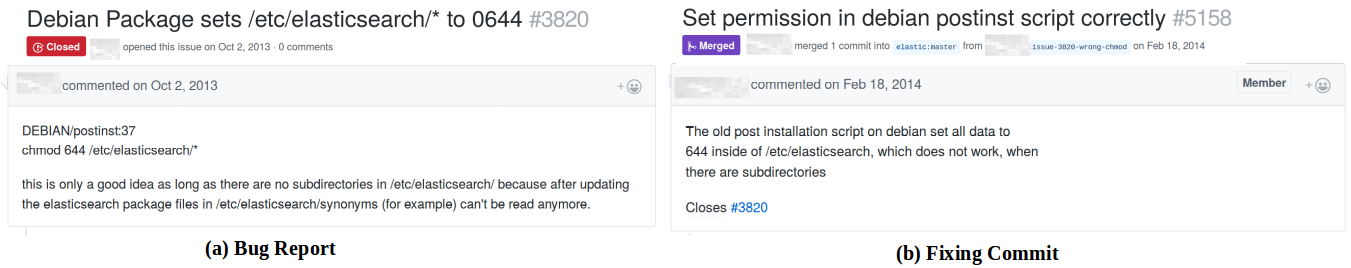
\includegraphics[width=\columnwidth]{img/subdirectories.png}
\caption{Bug caused after changing the version of the software.}
\label{fig:subdirectories}       % Give a unique label
\end{figure}

\begin{figure}[ht]
\centering
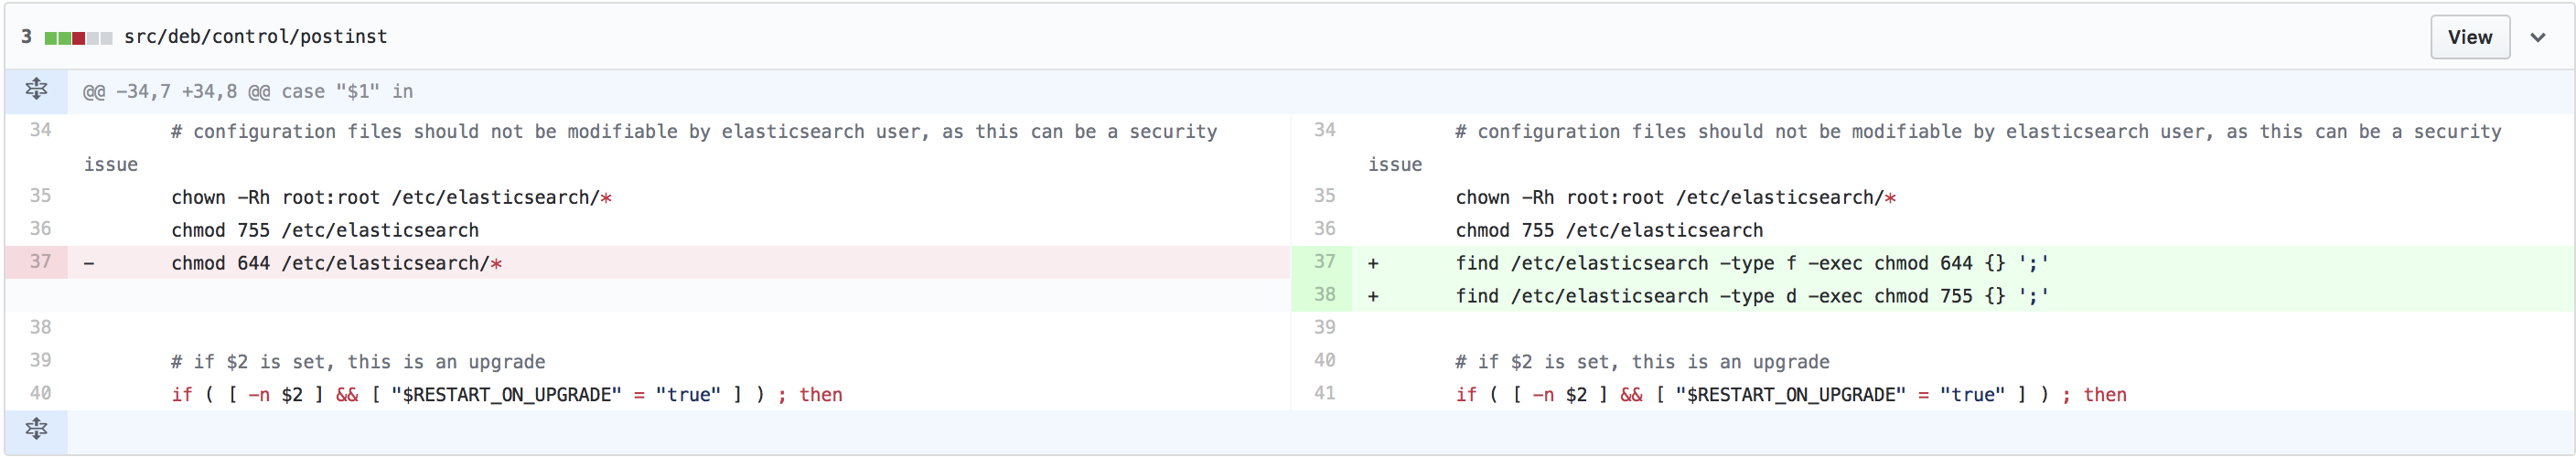
\includegraphics[width=\columnwidth]{img/subdirectoriesfix.png}
\caption{diff of the Bug-Fixing Commit}
\label{fig:subdirectoriesfix}       % Give a unique label
\end{figure}


%Ejemplo de las APIs
The second example is bug \#3551\footnote{https://github.com/elastic/elasticsearch/issues/3551} which is also from ElasticSearch. On the left of Figure~\ref{fig:java} the bug report description is shown and on the right there is the message description of its bug fixing commit. Below, Figure~\ref{fig:javafix} shows the code in the bug-fixing commit \emph{8668479b9}\footnote{https://github.com/elastic/elasticsearch/commit/8668479b9}. The bug report describes a bug when downloading a site plugin from Github. In this case, the dependency of the source code of ElasticSearch on a third-party as Github it is what caused the bug. At some point the API of Github changed and, as a consequence, the plugin to download \emph{ulr} from master zip file does not work, as a result the bug-fixing commit will have to pass the path of Github in order to fix the bug. In Figure~\ref{fig:javafix}, it can be observed that to fix the bug, the developer modified two lines \emph{182 and 196}. These modifications however do not mean that the lines were inserting a bug at the moment of the change, but  these lines manifested the failure due to other factors (i.e., a change in a third-party). Thus, as in the above example, none of the previous commits were inserting the bug, so it can be only identified after the change when the bug starts to manifest, meaning it is only possible to identify the First-Failing Commit.
%and the description of its bug-fixing commit \#18140
\begin{figure}[ht]
\centering
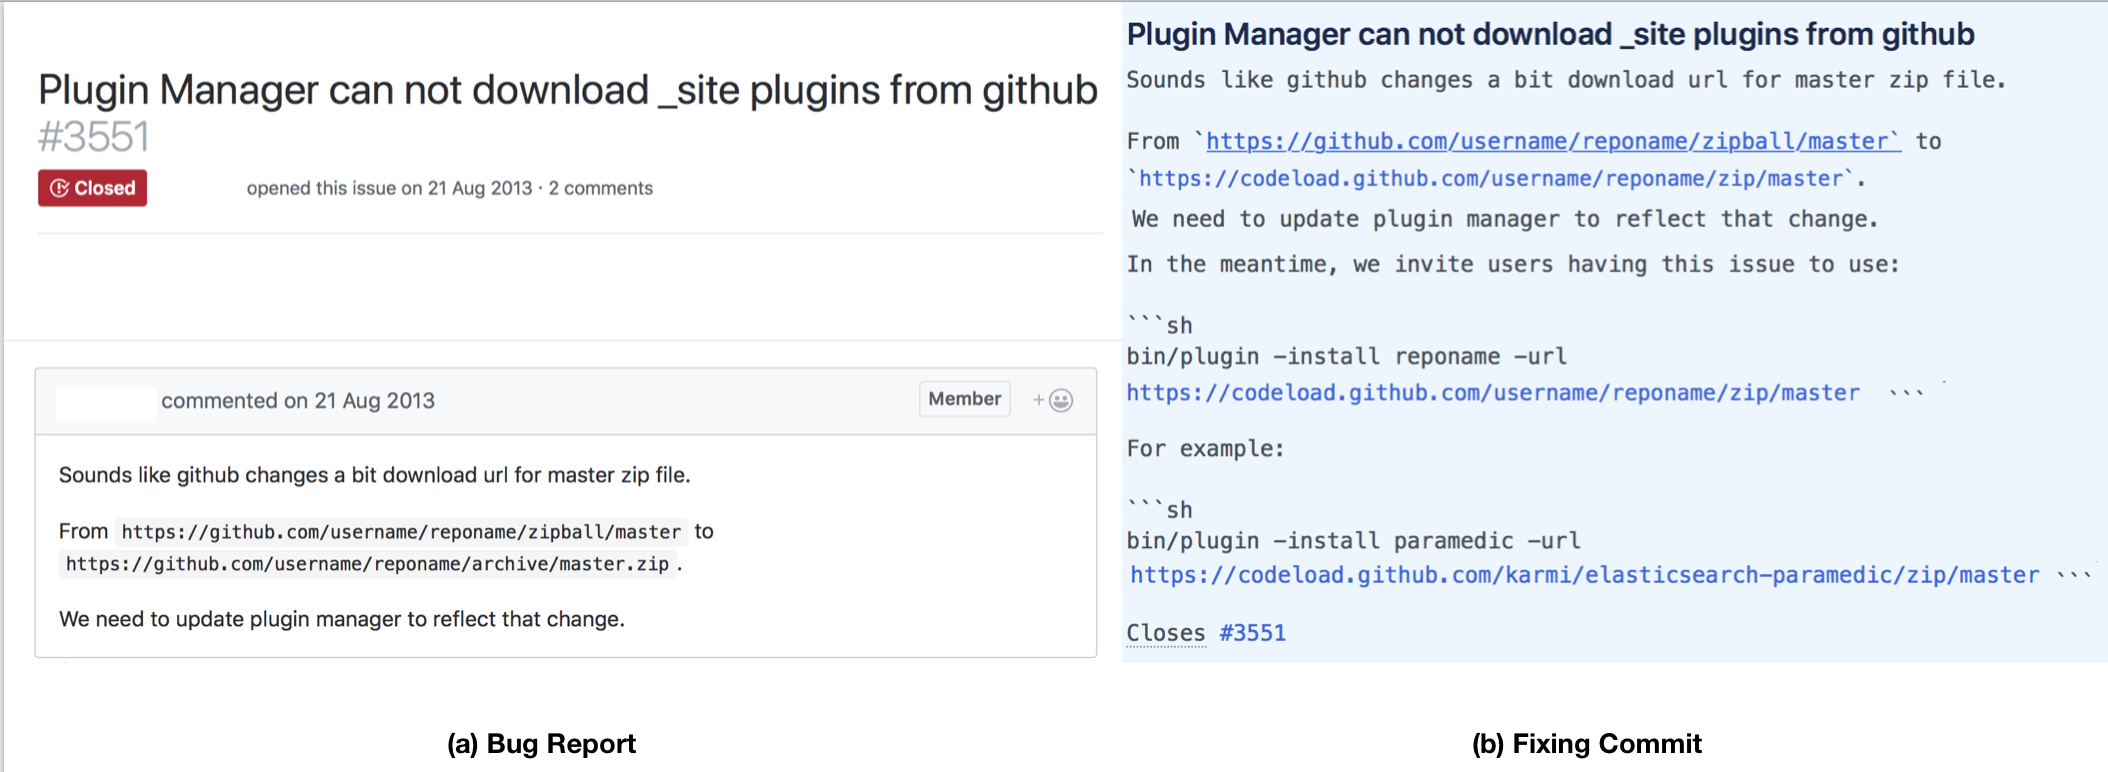
\includegraphics[width=\columnwidth]{img/github.png}
\caption{Bug caused by an external artifact.}
\label{fig:java}       % Give a unique label
\end{figure}

\begin{figure}[ht]
\centering
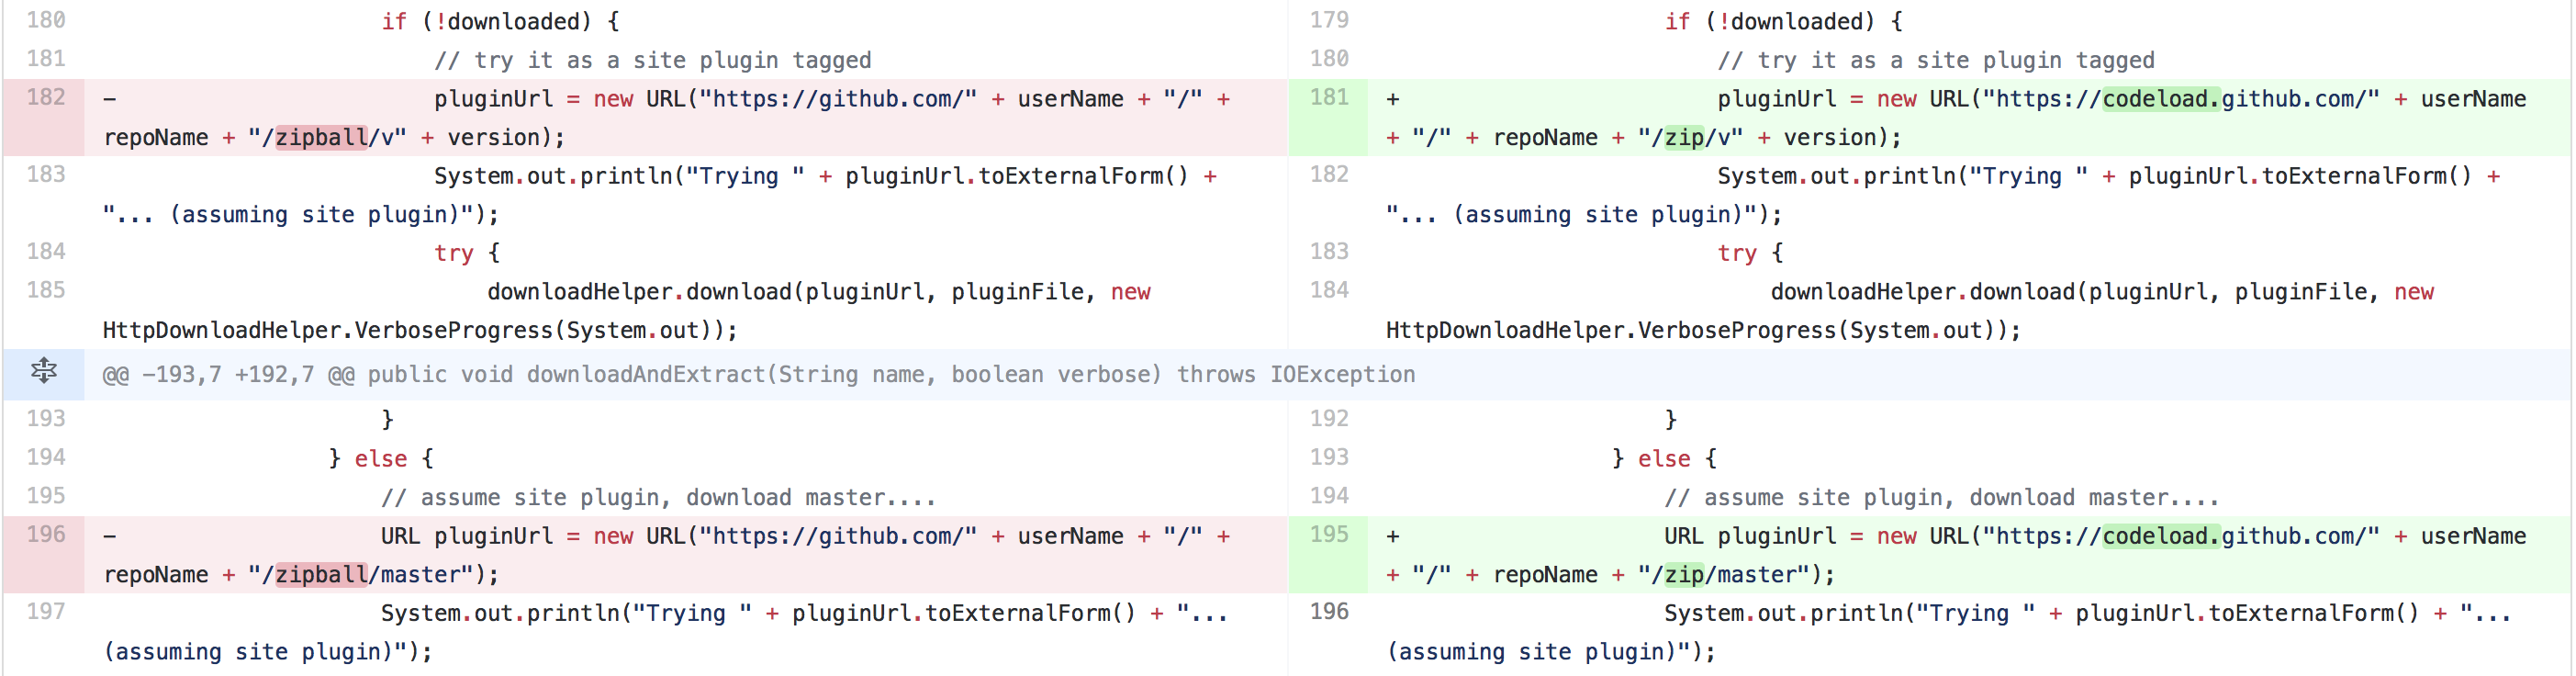
\includegraphics[width=\columnwidth]{img/githubfix.png}
\caption{diff of the Bug-Fixing Commit.}
\label{fig:javafix}       % Give a unique label
\end{figure}

%Ejemplo de windows
Finally, the last example is the bug \#1305897\footnote{https://bugs.launchpad.net/nova/+bug/1305897} from Nova. Figure~\ref{fig:windowsissue} shows the description of the bug report in Launchpad. According to it, the bug was caused by an incompatibility between the software and hardware used. The bug appeared when an option is enabled by default in the VMs;  this option depends on the underlying hardware. Thus, when a user has Windows Server 2012, this option is enabled and it causes the Hyper-V driver to be not aware of the constraint, therefore it becomes not possible to boot new VMs. Figure~\ref{fig:windowsissuefix} shows the Bug-Fixing Commit that modified line \emph{92} and inserted two new lines into the source code. The modification added a new argument into a function. This argument is used in the added lines to check the constrain that caused the bug. Thus, the change that introduced the modified line in the bug-fixing commit cannot be labeled as the Bug-Introduction-Commit. This is because the bug manifests depending on the environment. In this example, the current approaches also identify a false positive Bug-Introduction Commit, because it was correct in the moment of their insertion, while assuming that the developers were not aware of this issue and their intentions were not to make the software compatible in all the possible scenarios.
\begin{figure}[ht]
\centering
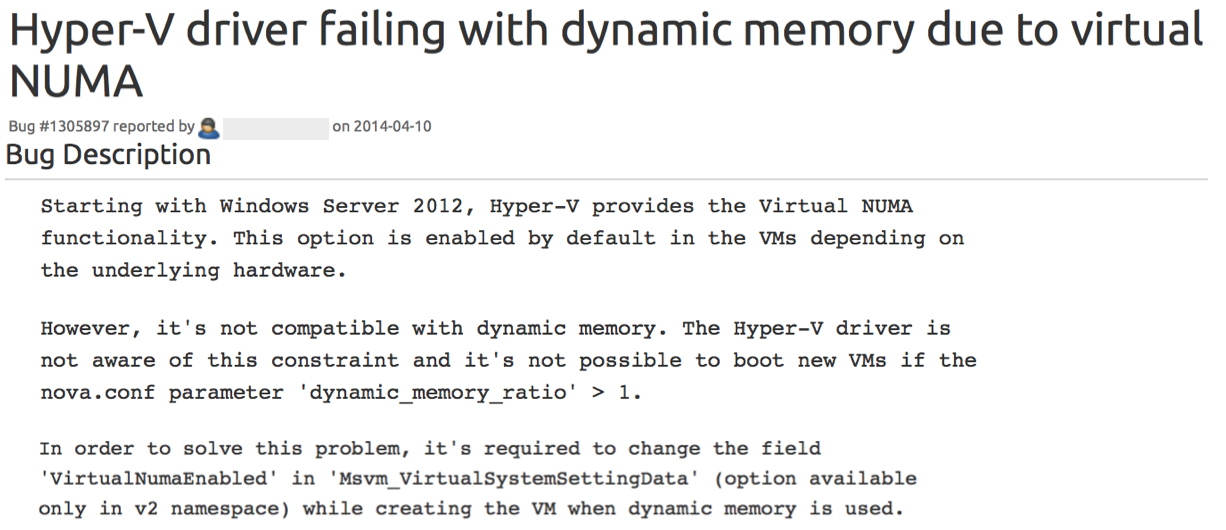
\includegraphics[width=\columnwidth]{img/windowsIssue.png}
\caption{Bug caused by the operating system where the code is being used.}
\label{fig:windowsissue}       % Give a unique label
\end{figure}

\begin{figure}[ht]
\centering
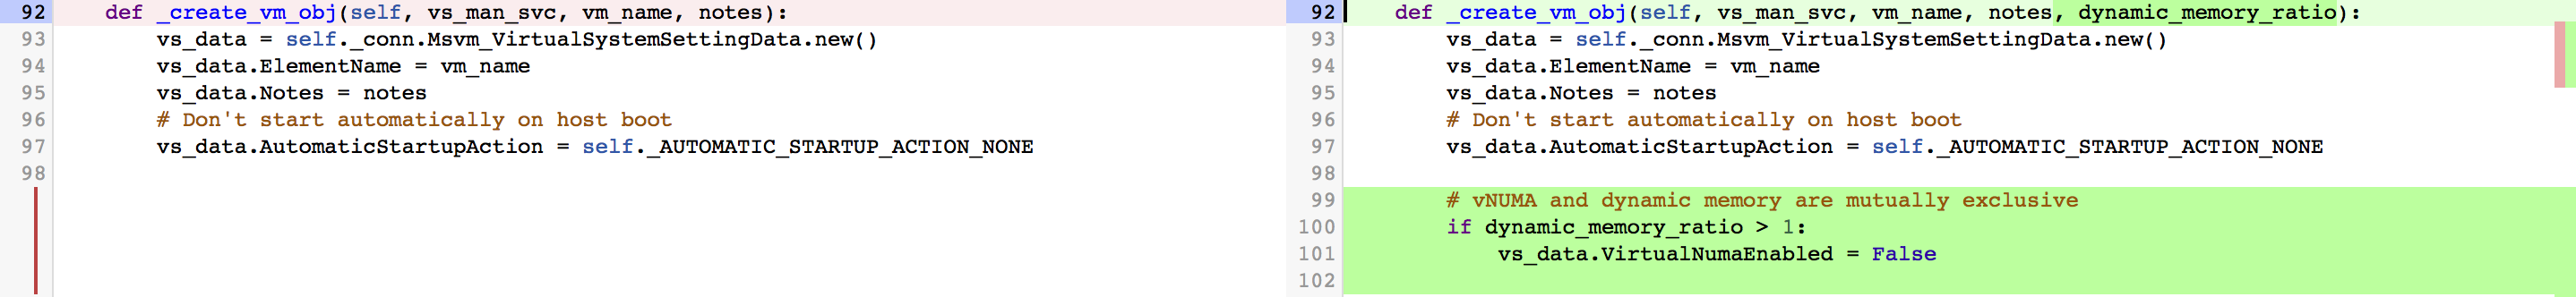
\includegraphics[width=\columnwidth]{img/windowsIssuefix.png}
\caption{Bug caused by an operating system where the code is being used.}
\label{fig:windowsissuefix}       % Give a unique label
\end{figure}

From the demonstration of the real real examples form ElasticSearch and Nova, it is clear that there are cases where  the effect of the external changes, the new requirements and incompatibilities are what caused the failure. These bugs self-manifest without the necessity of having any previous or ancestral changes to introduce the bug into the source code. Hence, in order to find the origin of a bug, not only the fixed lines in the bug-fixing commit  have to be taken into account, the dependencies or ecosystem of such lines must also be considered. It is important to also note that there is no sense to lie a blame on a change as the cause of the bug, because they did not inserted them. However, only the fist change that manifest the bug may be defined within the context of a concrete test system that contains all the dependencies.

\section{The Role of Version Control Systems in the Identification of BIC}
\label{subsec:VCS}

This thesis has considerable interest in version control systems \emph{VCS}, since it provides researchers with all the necessary data to analyze and understand the moment when a bug is introduced by first time. It is also the moment when a bug manifests in the project by first time. Thus, it is important to understand how they work and how developers and practitioners have been used them over the last decades. Furthermore, there is special interest for these systems because the selected projects to be analyzed in this thesis use a VCS. It is also because the vast majority of approaches for finding the bug introducing commit and for predict future bugs use them. 

VCS were developed to coordinate the shared access between many developers to the documents and files. These systems allow for simultaneous development of many branches and can detect any change committed in the source code. Then, these changes are saved along with the information of the timestamp and the identifier of the developer that make them. The VCS of a project keeps track of every modification to the source code and allow developers to turn back to any previous moment and compare earlier versions of the code. They can also revert to the last modification or return to a specific version of the project.

The most common use of these systems is to develop software, but they are also used in content management systems. The best-known VCS are Apache \emph{Subversion (SVN)} and \emph{Git}. The web-based hosting service for Git is GitHub\footnote{https://github.com/}, whereas RiouxSVN\footnote{https://riouxsvn.com/} hosts SVN. Although, Mercurial\footnote{https://www.mercurial-scm.org}, Bazaar\footnote{http://bazaar.canonical.com/en/} and CVS\footnote{https://www.nongnu.org/cvs/} are also well known. These VCS can be classified into two classes; \emph{Centralized VCS} that keep the history of changes on a central server where everyone requests the latest version and pushes the latest changes to.  \emph{Distributed VCS} in when everyone has a local copy of the entire repository. Thus, it is not necessary to push changes to the work all time, it allows for anyone to sync with any other team member.

SVN is a centralized VCS with a unique central repository which hosts all the data for the users. This disables two users from being unable to edit a file at the same time, and that every single change has to be pushed forward immediately.  Figure~\ref{fig:subversion} shows how a SVN project works, in the picture there are three developers with access to modify the files; when developer \emph{A.} modifies a file she has to push the changes to the central repository. Developer \emph{B.} and \emph{C.} only have the new state of the project after pulling the central repository, furthermore they cannot make any changes to the same file as developer \emph{A.}. While developer \emph{A.} is making changes to a file, other developers are unable to make any modification until developer \emph{A.} finishes and pushes the changes. 

\begin{figure}[ht]
\centering
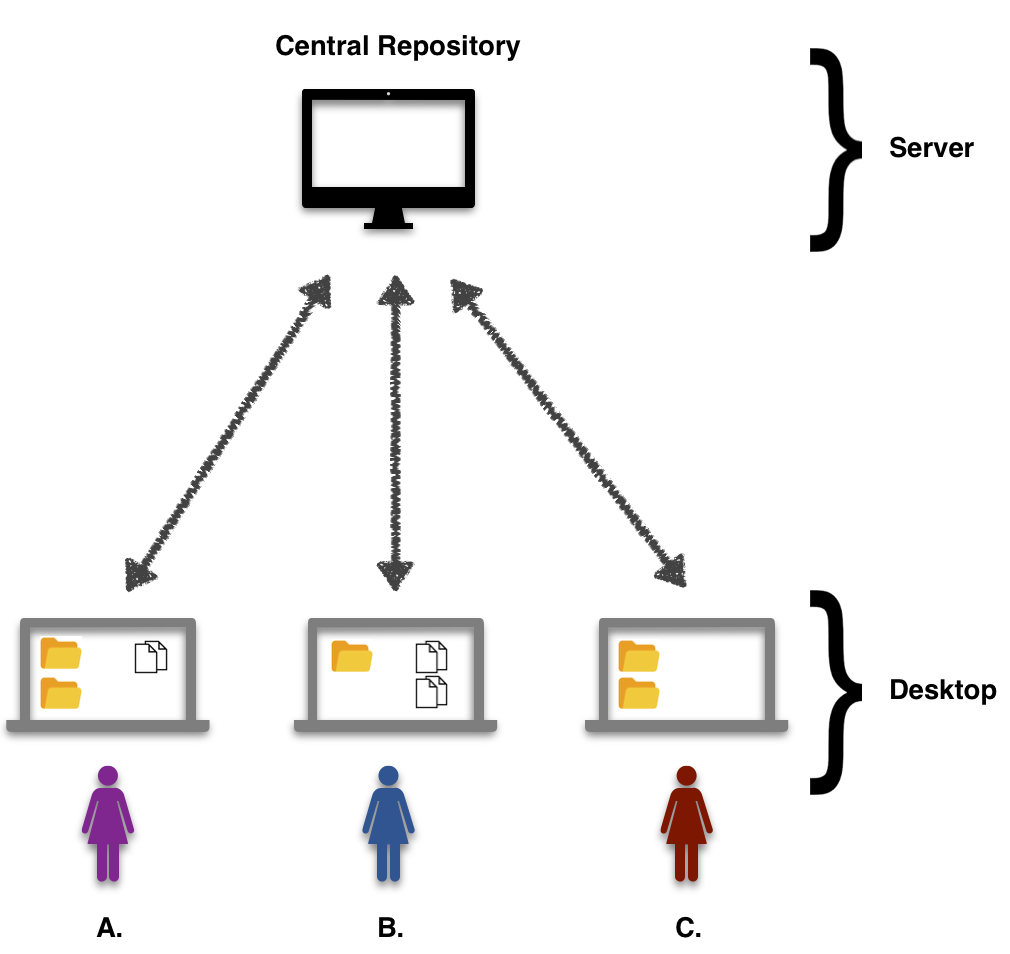
\includegraphics[height= 6cm]{img/subversion.png}
\caption{subversion}
\label{fig:subversion}       % Give a unique label
\end{figure}

On the contrary, Git is a decentralized VCS, it has a unique central repository but each developer has their own local repository. Thus, developers can push their code to their private repository, while getting all the benefit of VCS. They can make their code better after some changes, before pushing the changes from their repository to the central repository and letting other people use their new code. Figure~\ref{fig:git-mercurial} presents how a Git project works, in the picture there are three developers with access to modify the files, each developer has a local copy of the central repository in their computer. Thus, developer \emph{A.}, \emph{B.} and \emph{C.} can modify the files as many times as they want before pushing the changes to the central repository. This may cause the developers to be in different states of the same project in their local repository because they have not pushed or pulled frequently. In Git, same files can be modified at the same time, however if the developers have changed the same line, the system enters into a conflict that has to be solved before developers can continue committing changes.

\begin{figure}[ht]
\centering
\includegraphics[height= 6cm]{img/git-mercurial.png}
\caption{git-mercurial}
\label{fig:git-mercurial}       % Give a unique label
\end{figure}


Unfortunately, the current approaches used to identify the Bug-Introduction Commits are not understood for the \emph{real} moment of inserting a buggy line in the source code, the cause of the bug, and it force practitioners to apply these approaches to all the projects without regarding the nature of the bug, the dependencies of the bug or even whether they use SVN or Git. It is important to understand why the VCS are relevant when using the approaches to find the \BIC, specifically, because some of the approaches were developed to be used in SVN and they understand the branches in a different way than Git. For example, a branch in Git is only a pointer to some commit which can move and it causes the complete loss of the previous states where this is impossible in SVN. In other words, git does not keep a relationship of the changes setting in time, thus the approaches that use temporally windows to remove false positives or have faith that the precedence between commits is set by dates are not suitable in Git. Furthermore, another characteristic of Git is also the wide variety of commands at our disposal such as \emph{git diff, git remote, git bisect or git blame}. However, some of these options such as \emph{git merge, git rebase or git squash} can alter the natural order of the commits, in the sense that when the history of the commits are viewed using \emph{git log}, it may occur that the commits are not sorted by dates as presumed form the beginning. Hence, the use of Git also can affect the correct identification of Bug-Introducing Commits, and since the project analyzed in this thesis use Git as VCS, how these command affect the identification of the origin of a bug is described in detail. %This happens because of some commands such as \emph{git merge, git rebase or git squash} that might alter the natural order of the commits
%Moreover, as we have explained before, it is not fair to blame changes as the \BIC when in fact they are not the real cause of the bug, so to be more accurate in the results and can learn from the history of the projects taking into account all the factors around, we have proposed to find the \FFC instead of the BIC and, furthermore we must understand that this \FFC has dependencies which help to comprehend the origin of the bug

%The projects that we have studied use Git as control version system. One of the characteristics of Git is also the wide variety of commands at our disposal such as git diff, git remote, git bisect or git blame. However, some options can alter the normal order of the commits, in the sense that when you look at the history of the commits using \emph{git log}, it may happen that the commits are not sorted by dates as we would think in the beginning. This happens because of some commands such as \emph{git merge, git rebase or git squash} that might alter the natural order of the commits.

To better understand how Git might affect the identification of \BIC, this thesis explains three common scenarios with different commands available in Git. All of the scenarios use the same simple example. In the example, the repository only has two diverging branches, the master branch and the feature branch. The commit hashes\footnote{a unique 40 character string generated by the SHA-1 algorithm which takes some data as input and generates the hash} are represented with integers, and in addition, these integers also represent timestamps, where a smaller number means an earlier commit.

\paragraph{Git Merge:} The first scenario is when a developer uses Git Merge. This command is used to create a new commit. This new commit has two different parents and it is the only commit with this characteristic. The only time that Git Merge does not create a new commit is when the developer use the \emph{fast-forward merge} command. This situation occurs when there are no commits in another branch. Figure~\ref{fig:gitmerge} shows the repository before and after the merge. In this case, to see the precedence between commits, \emph{git log} can be typed after merging the branch and the result is a lineal log sorted by date: 7,6,5,4,3,2,1 .
\begin{figure}[ht]
\centering
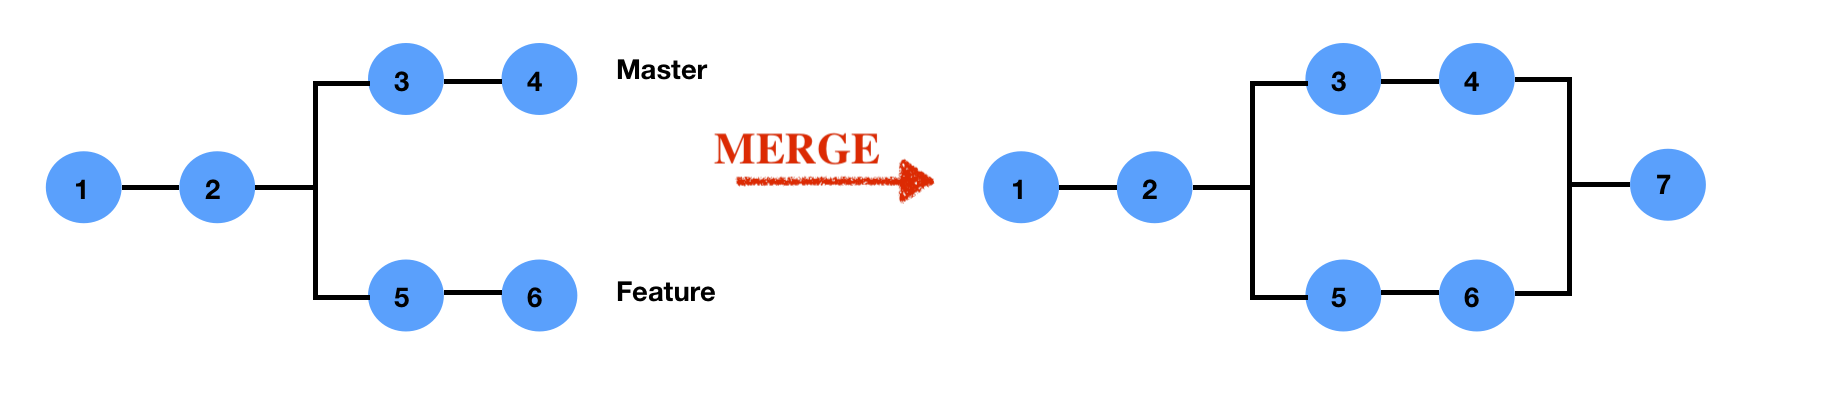
\includegraphics[width=\columnwidth]{img/gitmerge.png}
\caption{git-merge}
\label{fig:gitmerge}       % Give a unique label
\end{figure}

\paragraph{Git Rebase:} The second scenario is when a developer uses Git Rebase. This command recreates the work made from one branch onto another. For example, if a developer wants to rebase the master branch in the feature branch, for every commit that the master branch has that is not in feature branch, a new commit will be created on top of the feature branch. The Figure~\ref{fig:gitrebase} shows the output before and after the rebase from master branch onto feature. In this case, git rebase has moved changes 3 and 4 to the master branch, and it has changed the hash in order to add a new one. In this case, to see the precedence between commits, \emph{git log} can be typed after rebasing, the result is a lineal log that is not sorted by date: 8, 7, 6, 5, 2, 1.
\begin{figure}[ht]
\centering
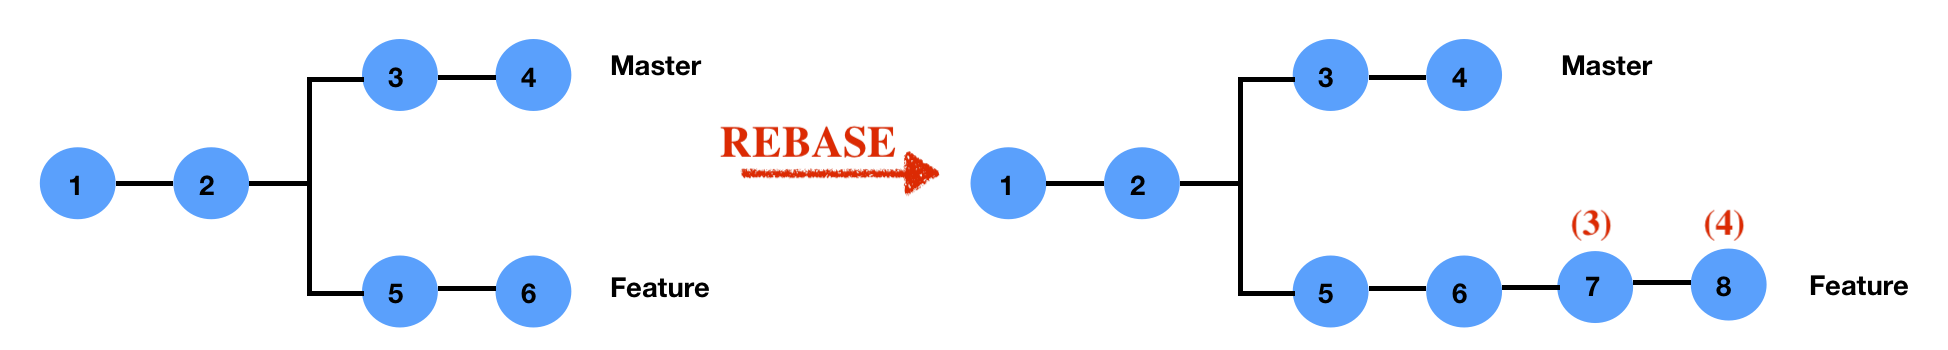
\includegraphics[width=\columnwidth]{img/gitrebase.png}
\caption{git-rebase}
\label{fig:gitrebase}       % Give a unique label
\end{figure}

\paragraph{Git Squash}  The third scenario is when a developer uses Git Squash. This command takes a series of commits and squash them down into a single commit. The main problem of this option is that the authorship of each commit squashed is lost, because these commits disappear from the history. Figure~\ref{fig:gitsquash} shows the output before and after squashing commits 5 and 6 from feature branch onto master. In this case, Git Squash has combined changes 5 and 6 to create a new commit 7,  this commit is then merged with the master branch. In this case, to see the precedence between commits we can type \emph{git log} after squashing, the result is a lineal log  that is sorted by date:  7, 4, 3, 2, 1.
\begin{figure}[ht]
\centering
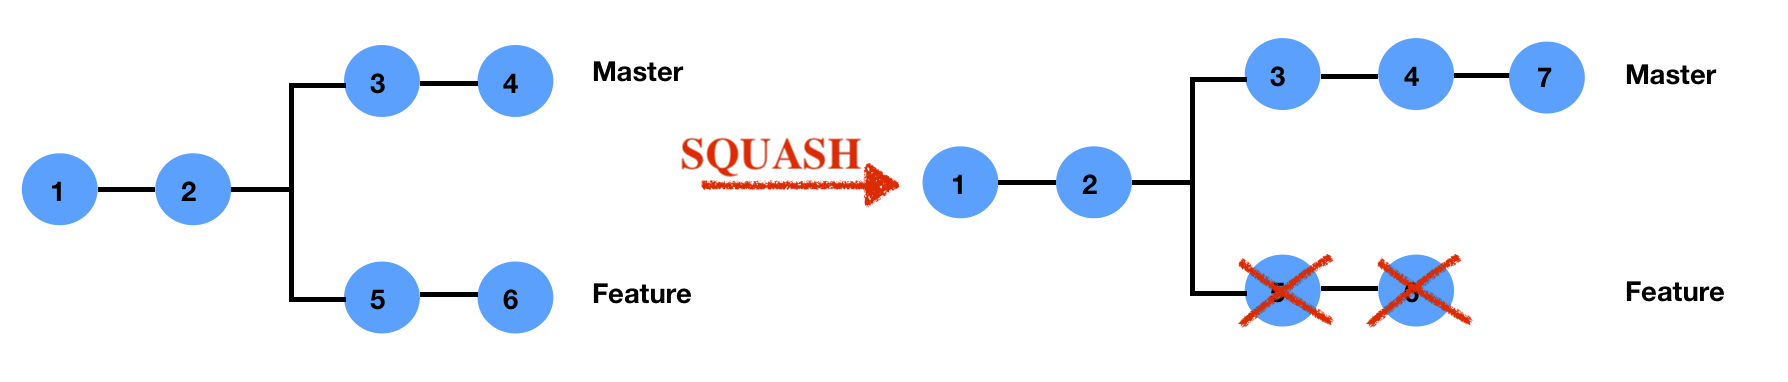
\includegraphics[width=\columnwidth]{img/gitsquash.png}
\caption{git-squash}
\label{fig:gitsquash}       % Give a unique label
\end{figure}

At the end, these types of tool facilitate the interaction between developers when a large number of them work in the same project. They are even more useful when the developers are distributed around the world working in different time zones. However, in order to find the Bug-Introduction Commit, it must be kept in mind that some available options in Git might hint the \emph{real} moment of bug introduction because some commands such as \emph{git merge, git rebase or git squash} that might alter the natural order of the commits and its origin. %Moreover, as we have explained before, it is not accurate to blame changes as the \BIC when in fact they are not the cause of the bug, to be more accurate in the results and can learn from the history of the projects taking into account all the factors around, we have proposed to find the \FFC instead of the BIC and, furthermore we must understand that this \FFC has dependencies which help to comprehend the origin of the bug


%%%%%%%%%%%%%%%%%%%%%%%%%%%%%%%%%%%%%%%%%%%%%%%%%%%%%%%%%%%%%%%%%%%%%%%%%%%%%%%%
%%%%%%%%%%%%%%%%%%%%%%%%%%%%%%%%%%%%%%%%%%%%%%%%%%%%%%%%%%%%%%%%%%%%%%%%%%%%%%%%
% CREDIBILITY IN THE SZZ %
%%%%%%%%%%%%%%%%%%%%%%%%%%%%%%%%%%%%%%%%%%%%%%%%%%%%%%%%%%%%%%%%%%%%%%%%%%%%%%%%

\cleardoublepage
\chapter{Reproducibility and Credibility of the SZZ}
\label{chap:credibility}

Reproducibility of Empirical Software Engineering (ESE) studies is an essential part for improving their credibility, as it offers the opportunity for the research community to verify, evaluate and improve their research outcomes where concerns related to the reliability of the results may arise. Furthermore, it is one of the fundamental characteristics of the scientific method~\cite{gonzalez2012reproducibility}. Juristo and Vegas state that reproducibility ``is important to increase and consolidate the body of empirical knowledge''~\cite{juristo2009using}, and Robles shows that reproducibility may be hindered by many factors~\cite{robles2010replicating}. 

Through this thesis, we adopt the definition of reproducibility by Madeyski and Kitchenham~\cite{madeyski2017would} which claims that ``reproducible research is the extent to which the report of a specific scientific  study can be reproduced (in  effect, compiled) from a reported text, data and analysis procedures, and thus can be validated by other researchers''. Although there are differences between reproducibility and replication, we assume that a research work is more likely to be replicated when it incorporates means of reproducibility. However, reproducibility  (and by extension credibility, since multiple replications of an experiment increase it~\cite{juristo2009using}) may be a challenging work, as access to data sources, use of specific tools, availability of detailed documentation has to be handled. Thus, detecting elements that my hinder reproducibility should help strengthen the credibility of the empirical studies~\cite{perry2000empirical}. 

This chapter addresses how the scientific practice of the ESE research community affects the reproducibility and credibility of the results of studies that use the SZZ algorithm, published in 2005 by {\'S}liwerski, Zimmermann and Zeller~\cite{sliwerski2005changes}  to detect the origin of a bug. The goal is to give a detailed description of the algorithm and explain its limitations and enhancements; then we detail the Systematic Literature Review \emph{(SLR)} in the credibility and reproducibility of the SZZ. Notice that this section is based on the manuscript ``Reproducibility and credibility in empirical software engineering: A case study based on a systematic literature review of the use of the SZZ algorithm" published in the \emph{Information and Software Technology} Journal. Regarding further details about this section, please refer to the paper.


\section{Description of the SZZ algorithm.}
\label{subsec:SZZ algorithm}
%Description of SZZ
In software engineering research, the SZZ algorithm is a popular algorithm for identifying bug-introducing changes~\cite{da2016framework}. SZZ relies on historical data from version control systems and bug tracking systems to identify change sets in the source code that induce bug fixes. The algorithm addresses two different problems. The first problem is related to the linkage between the VCS and the issue tracking system in order to identify the bug-fixing commit; the second problem is related to the identification of the bug-introducing commit.

In the first part, the algorithm identifies, by means of a set of heuristics, bug-fixing commits through using a technique that matches commits with bug reports labeled as \emph{fixed} in the bug tracking system. Therefore it uses regular expressions to identify bug numbers and keywords in the commit messages that are likely to point out a real bug fixing change. This is possible since many projects have adopted the policy of recording the bug report number in the message of the commit that fixed the bug. Thus, the algorithm splits every log message into a stream of tokens to find the potential \emph{bug number} with the use of regular expressions. For instance, the algorithm looks for keywords such as \emph{fix(e[ed]), bugs, defects, patch} followed by a number.

The second part of the algorithm is concerned with the identification of the bug-introducing commit(s). The algorithm employs the \textit{diff} functionality implemented in source code management systems to determine the lines that have been changed (to fix the bug) between the fix commit version and its previous version. Then, using the \textit{annotate/blame} functionality, SZZ is able to locate who modified or deleted those lines for the last time in previous commit(s), and, whether they were committed before the bug was reported; those change(s) are flagged as suspicious of being the bug-introducing commit(s).

As an example, Figure~\ref{fig:code} shows three different snapshots o at different times  and Figure~\ref{fig:history-log} shows when and who changed the code in each commit. The first change is made by Alice on the 1\textsuperscript{st} of June where \textit{12cf3s}, is the bug-introducing commit; the bug is introduced in line 21 because the condition for the \emph{if} statement is used incorrectly. The bug was then reported on the 2\textsuperscript{nd} of June. After that, Becky made the second change on the 3\textsuperscript{rd} of June, \textit{4asd23f}, which added code to the \emph{foo()} function in lines 24, 25 and 26. Finally, the third change, \textit{21esd33} is made by Cloe on the 5\textsuperscript{th} of June. The change fixed the bug by modifying two lines: the buggy line 21 and the clean line 25. In the bug-fixing commit, the modification of line 25 was purely semantic because the line retains with the same behavior from before its modification, in both cases the variable \emph{bar} is incremented by one.

Figure~\ref{fig:SZZalgorithm} shows how the algorithm works. First, after the report of the bug notification \emph{\#159} in the issue tracking system, the algorithm identifies the bug fixing commit \textit{21esd33} by looking in the logs for a commit with the commit message containing bug number \emph{\#159}. After that, the second part of the algorithm searches for the bug-introducing commit by using the \emph{diff} tool and \emph{annotate/blame} tool in each of the lines modified in the bug-fixing commit. In this example, lines 21 and 25 have been changed in the bug fixing commit in order to fix the bug, thus both lines are marked for suspicion of being the ones where the bug was introduced. These lines have been inserted in two different commits, however, as line 25 was introduced in a commit after the bug was reported, the algorithm removed it from the list of suspicious bug-introducing commits. Consequently, only the commit that last modified line 21 can be blamed as the bug-introducing commit. Thus, in this case, the SZZ algorithm correctly points out that \textit{12cf3s} is the bug introducing change.

Unfortunately, the algorithm does not always behave as demonstrated in the above example. In some scenarios, the practitioners can notify some of the shortcomings which may cause the malfunction. These shortcomings, as well as some examples of the malfunction of the SZZ are detailed in the next section.

\begin{figure}
\centering
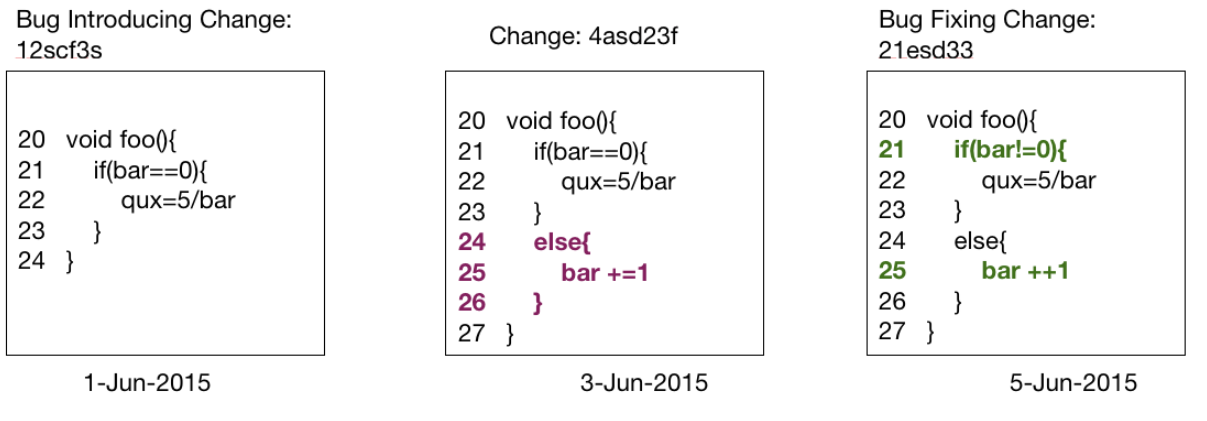
\includegraphics[width=\columnwidth]{img/code.png}
\caption{Example of changes committed in a file, the first change is the bug introducing change and the third change is the bug fixing change. }
\label{fig:code}       % Give a unique label
\end{figure}

\begin{figure}
\centering
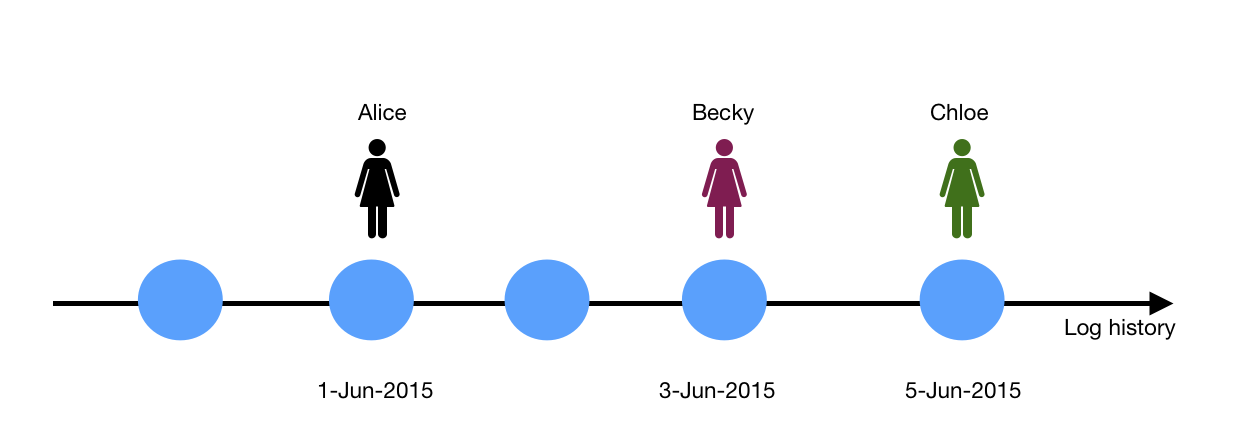
\includegraphics[width=\columnwidth]{img/history-log.png}
\caption{The changes were committed by Alice, Becky and Chloe in different days. }
\label{fig:history-log}       % Give a unique label
\end{figure}

\begin{figure}
\centering
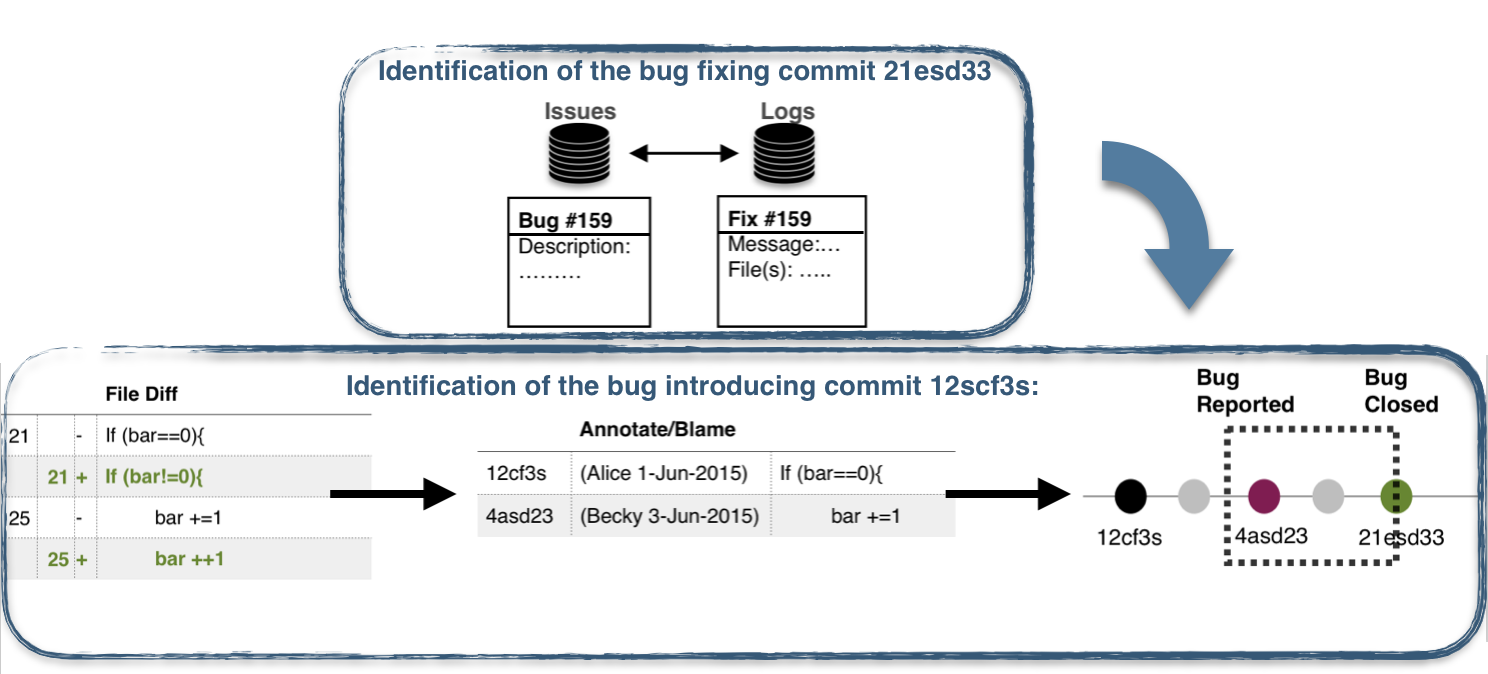
\includegraphics[width=\columnwidth]{img/SZZalgorithm.png}
\caption{First and Second part of the SZZ algorithm}
\label{fig:SZZalgorithm}       % Give a unique label
\end{figure}


\section{Shortcomings of the SZZ Algorithm:}
\label{subsec:limitations}

Despite SZZ being largely used in ESE to locate bug origins, it presents some shortcomings which makes it error prone. Table~\ref{shortcomingsSZZ} offers a detailed overview of the shortcomings in SZZ as reported in the literature. Some of them have been previously explained in the Chapter \ref{chap:context}, however, in this section they are described with examples based on the illustrative Figure~\ref{fig:code}.

In the first part of the algorithm the limitation lies in how bug reports are linked to commits. If the fixing commit (in the versioning system) does not contain a reference to the bug (usually the reference is the unique id assigned by the bug tracking system, but it could be certain keywords as well), it is very difficult to link both data sources. Sometimes this linking is incorrect as the bug fixing commit do not correspond to the bug report. If the fixing commit is not identified, the bug-introducing commit cannot be determined and this causes a \emph{false negative}\footnote{The definition of false negative has been addressed in the previous Chapter \ref{chap:context}}. Studies have demonstrated that 33.8\%~\cite{herzig2013s} to 40\% \cite{rodriguez2016bugtracking} of the bugs in the issue tracker are misclassified, i.e., issues categorized as bugs are actually functionality requests or refactoring suggestions. A false positive\footnote{The definition of false positive has been addressed in the previous Chapter \ref{chap:context}} occurs when a bug report does not describe a real bug, but a fixing commit is still linked to it. Herzig et al. pointed out that 39\% of files marked as defective have never had a bug~\cite{herzig2013s}.

%Furthermore, another issue to take into account is systematic bias: some studies have demonstrated that two out of five issues are misclassified~\cite{herzig2013s},\cite{rodriguez2016bugtracking}. Thus, we have a \emph{false positive} when a bug report does not describe a \emph{real} bug, but a fixing commit is linked to it.

In the second part of the algorithm, lines might be incorrectly identified by SZZ as the place for where the bug was introduced, causing a \emph{false positive}. It may also be that the buggy line was not analyzed by SZZ, producing a \emph{false negative}. In some cases, the bug had been introduced before the last change to the line; then, the history of the line has to be traced back until the \emph{true} source of the bug is found~\cite{williams2008szz}. An example of this can be found when SZZ flags changes to \emph{style} (i.e., non-semantic/syntactic changes such as changes to white spaces, indentation, comments, and some changes that split or merge lines of code) as bug-introducing commits~\cite{da2016framework}, or when a project allows \emph{commit squashing}, since this option removes authorship information resulting in more \emph{false positives}. It may also happen that the bug may have been caused by a change in another part of the system~\cite{german2009change}. A final possibility is that the bug fix modified the surrounding context rather than the problematic lines, thereby misleading the algorithm~\cite{davies2014comparing}.

%\gema{Explain what a false positive, false negative true positive and true negative means here.}
\begin{table}[!t]
% increase table row spacing, adjust to taste
\newcommand{\specialcell}[2][l]{%
  \begin{tabular}[#1]{@{}l@{}}#2\end{tabular}}
\renewcommand{\arraystretch}{0.8}
% if using array.sty, it might be a good idea to tweak the value of
%\extrarowheight as needed to properly center the text within the cells
\caption{Shortcomings that can lead to false negatives when using SZZ.}
\label{shortcomingsSZZ}
\centering
% Some packages, such as MDW tools, offer better commands for making tables
%% than the plain LaTeX2e tabular which is used here.
\begin{adjustbox}{max width=\textwidth}
\begin{tabular}{|l|l|l|}
\hline
Part & Type & Description    \\
\hline
\hline
\multirow{3}*{First part} & Incomplete mapping~\cite{bird2009fair}. & The fixing commit cannot be linked to the bug report. \\  \cline{2-3}
 & Inaccurate mapping~\cite{bissyande2013empirical}.& \specialcell{The fixing commit has been linked to a wrong bug report,\\ they don't correspond each other.} \\ \cline{2-3}
 & Systematic bias~\cite{bird2009fair}.& Linking fixing commits with no \emph{real} bug reports.\\ \hline
\multirow{6}*{Second part} &  Cosmetic changes, comments, etc~\cite{kim2006automatic}.& Variable renaming, indentation, split lines, etc.  \\  \cline{2-3}
 &  Added lines in fixing commits~\cite{da2016framework}.& The new lines cannot be tracked back.  \\  \cline{2-3}
 &  Long fixing commits~\cite{da2016framework}. & The larger the fix the more false positives. \\  \cline{2-3}
 &  Semantic level is weak~\cite{williams2008szz} & Changes with the same behavior are being blamed. \\  \cline{2-3}
 &  Clean changes~\cite{da2016framework}.& \specialcell{This changes start leading to bugs due to external changes \\or artifacts are being blamed.} \\  \cline{2-3}
 & Commit Squashing~\cite{gousios2013ghtorent}.&  \specialcell{This practice might hide the real bug introducing commit,\\ it combine/merge multiple commits into a single commit loosing authorship information.} \\  \hline
\hline
\end{tabular}
\end{adjustbox}
\end{table}

%\gema{More limitations:Many bug fixes involve touching hundreds or even thousands of lines of code, c.f., many of these lines are changed not because they are root causes but because they need to be modified to facilitate the treatment of the bug. }

\subsection{Some Examples:}
\label{subsec:examples}
To provide more insights on the reasons why SZZ identifies false positive commits, we explain three possible scenarios based on the example shown in Figure~\ref{fig:code} in where the algorithm identifies false bug-introducing commits. However, in these scenarios the day of the bug report has changed from the 2\textsuperscript{nd} of June to the 4\textsuperscript{th} of June. Thus, the bug was not reported after the second change was committed, and after applying the heuristics, the SZZ is unable to remove the commit made by Becky from the list of suspicious bug-introducing commits.

The first scenario is represented in the code of Figure~\ref{fig:code} and is related with the problem of identifying more than one bug-introducing commit, and how practitioners should behave. This example shows how after applying the algorithm, it identifies two commits as being the possible Bug-Introducing commits. While the commit made by Alice is correctly identified as a Bug-Introducing commit, the change made by Becky is a false positive because of two main reasons; i) she did not introduce any bug when the lines were committed and, ii) she modified the code but it maintained the same logic of its previous state where line 25 still increments one unit on the variable \emph{``bar"}.

The second scenario is represented in the code of Figure~\ref{fig:code2}. In this scenario, the semantic changes made by Becky are hiding the real Bug-Introduction Commit because she decided to replace the name of the variable \emph{``bar"}  for \emph{``people"}. Even though this change may appear to be inoffensive, it modified the variable name in the buggy line 21 hinting the true Bug-Introducing Commit. Thus, when applying the SZZ algorithm, the outcome is that the last commit which touched buggy line 21 is the commit made by Becky, when in fact, the bug was already in the line when Becky decided to change the name of the variable. In this case, the SZZ identifies a commit but it is not the Bug-Introducing Commit.

Finally, the third scenario is represented in the Figure~\ref{fig:code3}. It shows an example where unchanged lines introduced the bug. In this example, Alice wrote the function \emph{foo()}, but she forgot to add the \emph{if} condition which checks whether the variable \emph{``bar"} is not equal to 0, otherwise the logic in line 22 will fail because it is not allow to divide a variable between 0. Thus, in order to fix the bug Chloe added the \emph{if} condition in the bug-fixing commit. Therefore when the SZZ algorithm is applied, the outcome blames a wrong change as the Bug-Introducing Commit because the bug was fixed by adding a new line, and the SZZ algorithm cannot track back the line.

\begin{figure}
\centering
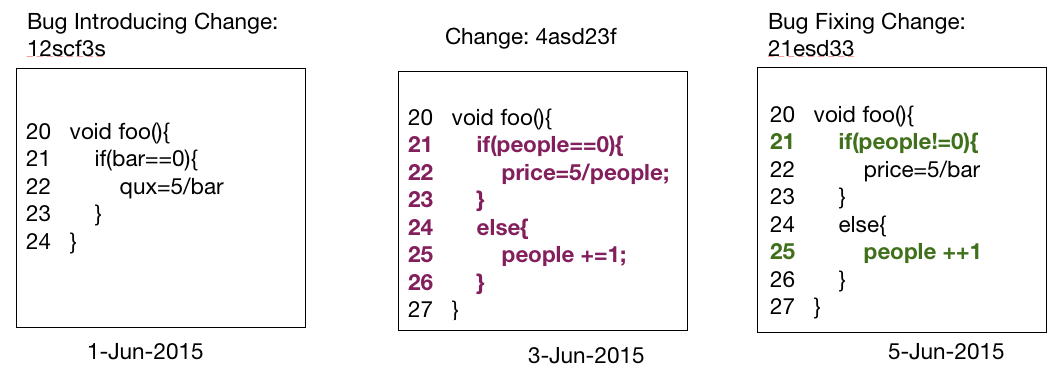
\includegraphics[width=\columnwidth]{img/code2.png}
\caption{Example where semantic changes in the buggy line hide the bug introducing change and the SZZ cannot identify it. }
\label{fig:code2}       % Give a unique label
\end{figure}

\begin{figure}
\centering
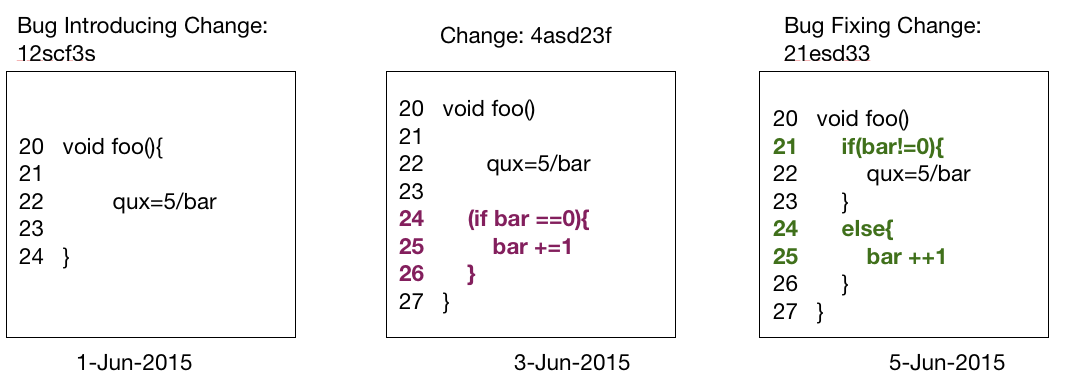
\includegraphics[width=\columnwidth]{img/code3.png}
\caption{Example where unchanged lines introduced the bug, and SZZ cannot identify the bug introducing commit.}
\label{fig:code3}       % Give a unique label
\end{figure}


\subsection{Enhancements of SZZ}
\label{subsec:Enhancements}
After describing the shortcomings of the SZZ found in the literature, the focus is now on how researchers have addressed them over time and in how far the enhancements have mitigate the problems.

The misclassification problem has been further investigated by researchers, aiming at mitigating the limitations found in the first part of SZZ~\cite{herzig2013s}, \cite{tan2015online} \cite{rodriguez2016bugtracking}. Tools and algorithms have been created based on the information from version control systems and issue tracking systems to map bug reports to fixing commits~\cite{wu2011relink},\cite{nguyen2012multi},\cite{le2015rclinker}, \cite{sun2017frlink}. As a result of these efforts, the first part of SZZ has seen how its accuracy has significantly increased. 

Related to the second part of SZZ, two main improvements have been proposed in the literature; they are referred to as SZZ-1 and SZZ-2:
\begin{itemize}
	\item \emph{SZZ-1}) Kim~\textit{et al.} suggest an SZZ implementation that excludes cosmetic changes, and propose the use of an \textit{annotation graph} instead of using \textit{annotate\footnote{Notice that annotate is used in SVN and blame is used in git.}}~\cite{kim2006automatic}.
	\item \emph{SZZ-2}) Williams and Spacco propose to use a mapping algorithm instead of annotation graphs; this approach uses weights to map the evolution of a source code line and ignores comments and formatting changes in the source code with the help of \texttt{DiffJ}, a Java-specific tool~\cite{williams2008szz}.
\end{itemize}

The second part of the algorithm however still has room for further improvements such as the work from Da Costa~\textit{et al.} who have created a framework to eliminate unlikely bug introducing changes from the outcome of SZZ. Their framework is based on a set of requirements that consider the dates of the suspicious commit and of the bug report~\cite{da2016framework}. By removing the commits that do not fulfill these requirements, the number of false positives provided by SZZ is lowered significantly.
. As can be seen, addressing the limitations of the SZZ often requires a manual, tedious validation process which can be impractical at times.

\section{Systematic Literature Review on the use of SZZ algorithm}
\label{subsec:SLR}

Through this subsection we present the Systematic Literature Review (SLR) on the use of the SZZ algorithm in 187 academic publications in order to address how the scientific practice of the ESE research community affects the reproducibility and credibility of the results. In particular, we want to address studies that use the SZZ algorithm, published in 2005 in ``When do changes induce fixes?'' by {\'S}liwerski, Zimmermann and Zeller~\cite{sliwerski2005changes} at the MSR workshop\footnote{MSR is today a working conference, but at that time it was a co-located workshop with ICSE in its second edition.}.  SZZ has been largely used in academia, counting, as of May 2018, with more than 610 citations in Google Scholar\footnote{https://scholar.google.es/scholar?cites=3875838236578562833}.

The purpose of a SLR is to identify, evaluate and interpret all available studies relevant to a particular topic, research question, or effect of interest~\cite{Kitchenham07guidelinesfor}. A SLR provides major information about the effects of a particular topic across a wide range of previous studies and empirical methods. As a result, a SLR should offer evidence with consistent results and suggest areas for further investigation. To address the SLR, we followed the approach proposed by Kitchenham and Charters~\cite{Kitchenham07guidelinesfor} in order to analyze the credibility and reproducibility of the SZZ algorithm. Therefore, we address the following  questions:
\begin{enumerate}
	\item \textbf{What is the impact of the SZZ algorithm in academia?} The SZZ algorithm has been shown to be a key factor in locating when a change induced fixing commits. However, many papers use only the first part of the algorithm to link bug fix reports to commits. As the second part of SZZ is shown to encompass significant threats, we identify only those publications that use both parts, or at least the second part, of the SZZ algorithm. In addition to this, we offer other metrics on the publications, such as the number of authors and the geographic diversity of the institutions they work for, in order to provide insight of how widespread the use of SZZ is.
	Furthermore, one of our goals addresses the maturity and diversity of the publications where SZZ has been used in order to understand its audience. We address the \emph{maturity} of a publication by analyzing whether it has been accepted in a workshop, a conference, a journal, or a top journal. Diversity is given by the number of distinct venues where publications using SZZ can be found.
	\item \textbf{Are studies that use SZZ reproducible?}  Reproducibility is a crucial aspect of a credible study in ESE~\cite{gonzalez2012reproducibility}. Piwowar~\emph{et al.} state that reproducibility improves the impact of research~\cite{piwowar2007sharing}. In addition, when a research work incorporates reproducibility, it is more likely to be replicated. However, there is evidence in the ESE literature that replicable studies are not common~\cite{robles2010replicating}. By providing a replication package (or a detailed description of the analysis and the environment and data used), the authors facilitate others to replicate or to reproduce their experiment, which increases the credibility of their results~\cite{juristo2009using}. In addition, replication packages help in the training of novice researchers~\cite{madeyski2017would}. To provide trustworthy results in ESE research, authors should offer a replication package and/or a detailed description of the research steps, and the environment and data used. This would allow others to reproduce or replicate their studies~\cite{gonzalez2012reproducibility}.
	\item \textbf{Do the publications mention the limitations of SZZ?} It has already been shown that limitations of SZZ are well-known in the research literature but there is still the question of how many papers report any of these. Therefore, this chapter also studies whether authors mention the limitations of SZZ that may affect their findings, be it in the \emph{description of the method}, in the \emph{threats to validity} or in the \emph{discussion}.
	\item \textbf{Are the improvements to SZZ (SZZ-1 and SZZ-2) used?} The improved versions of the original SZZ algorithm address some of its limitations. We analyze whether any of the improvements to the SZZ algorithm can be found in the primary studies included in the SLR. Thus, we search for any mention of their use, be it in the \emph{description of the method} or in the \emph{threats to validity}. Answering this research question enables further understanding on how authors who use SZZ behave given the limitations of SZZ.

\end{enumerate}

\subsection{Inclusion Criteria}
\label{subsec:Inclusion}
After enumerating the questions, we present the inclusion and exclusion criteria for the SLR. In addition, we describe the search strategy used for primary studies, the search sources and the reasons for removing papers from the list.
The inclusion criteria address all published studies written in English that cite either:
\begin{enumerate}
  \item The publication where SZZ was originally described,``When do changes induce fixes?"~\cite{sliwerski2005changes}, or
  \item (at least) one of the two publications with improved versions of the algorithm, ``Automatic Identification of Bug-Introducing Changes"~\cite{kim2006automatic} and ``SZZ Revisited: Verifying When Changes Induce Fixes"~\cite{williams2008szz}.  \end{enumerate}
 
There was no need to further investigate the references to the resulting set of publications (a process known as \emph{snowballing}): if one of these papers contained as well a reference to the papers that fit the inclusion criteria, it is assumed to be already in our sample. 

Before accepting a paper into the SLR, we excluded publications that are duplicates, i.e., a \emph{matured} version (usually a journal publication) of a \emph{less matured} version (conference, workshop, PhD thesis...). In those cases, we only considered the \emph{matured} version. When we found a short and a long version of the same publication, we have chosen the longer version.  However, in those cases where the publication is a PhD thesis and a related (peer-reviewed) publication exists in a workshop, conference or journal, the thesis is discarded in favor of the latter, because conference and journal publications are peer-reviewed whereas a PhD theses are not. Documents that are a \emph{false alarm} (i.e., not a \emph{real}, scientific publication) have also been excluded.

\subsection{Search Strategy used for Primary Studies}
\label{subsec:strategy}

The studies were identified using Google Scholar and Semantic Scholar as of November 8\textsuperscript{th} 2016. We have searched exclusively in Google Scholar and Semantic Scholar because of i) their high accuracy in locating citations, providing more results than other databases (from Table~\ref{tableSearch} it can be seen that they contain three times more citations than other platforms, such as the ACM Digital Library), and ii) because it was observed that they offer a superset of the other databases, i.e., it was checked checked that no publication in the other sources is missing from the list provided by Google Scholar and Semantic Scholar. However, Google Scholar gives many \emph{false alarms}, in the sense that they are not publications but slide sets, notes, etc. Examples of those \emph{false alarms} are ``Strathprints Institutional Repository"\footnote{\url{https://core.ac.uk/download/pdf/9032200.pdf}} or ``Home Research"\footnote{\url{http://ieeexplore.ieee.org/document/1382266/\#full-text-section}}), which was removed manually from our set. Some academic databases which are commonly used for SLRs, such as Scopus, could not be employed to gather citations, because SZZ was published at a time when MSR was a workshop, and thus the original publication~\cite{sliwerski2005changes} is not included in those databases.

\begin{table}[!t]
% increase table row spacing, adjust to taste
\renewcommand{\arraystretch}{0.8}
% if using array.sty, it might be a good idea to tweak the value of
%\extrarowheight as needed to properly center the text within the cells
\caption{Number of citations of the SZZ, SZZ-1 and SZZ-2 publications by research databases.}
\label{tableSearch}
\centering
% Some packages, such as MDW tools, offer better commands for making tables
%% than the plain LaTeX2e tabular which is used here.
\begin{adjustbox}{max width=\textwidth}
\begin{tabular}{|l|c|c|c|c|}
\hline
& Google Scholar & Semantic Scholar & ACM Digital Library & CiteSeerX \\
\hline
\hline
\# SZZ & 493 & 295 & 166 & 26 \\
\hline
\# SZZ-1 & 141 & 100 & 60 & 18 \\
\hline
\# SZZ-2 & 26 & 15 & 8 & 0 \\
\hline
\end{tabular}
\end{adjustbox}
\end{table}

\subsection{Study Selection Criteria and Procedures for Including and Excluding Primary Studies}
\label{subsec:selection}
Table~\ref{tableSelectedPapers} shows that our searches elicited 1,070 citation entries. After applying the inclusion criteria described above, a list of 458 papers was obtained. This process was performed by the first author. The process is objective, as it involves discarding false alarms, duplicates, and papers not written in English. 

Then, the first author analyzed the remaining 458 papers looking for the use of SZZ, SZZ-1 and SZZ-2 in the studies. This resulted in 193 papers being removed because of three main reasons: i) they only cited the algorithm as part of the introduction or related work but never used it, ii) they only cited the algorithm to support a claim during their results or the discussion, and iii) the papers were essays, systematic literature reviews or surveys. This process was discussed in advance by all the authors. The second author partially validated the process by analyzing a random subset comprising 10\% of the papers. The agreement between both authors was measured using Cohen's Kappa coefficient, resultingv in a value of 1 (perfect agreement). These papers were removed on the basis that they do not answer our research questions. After this process 273 papers were included in this SLR.

\begin{table}[!t]
% increase table row spacing, adjust to taste
\renewcommand{\arraystretch}{0.8}
% if using array.sty, it might be a good idea to tweak the value of
%\extrarowheight as needed to properly center the text within the cells
\caption{Number of papers that have cited the SZZ, SZZ-1 and SZZ-2 publications by joining the research databases Google Scholar and Semantic Scholar during each stage of the selection process.}
\label{tableSelectedPapers}
\centering
% Some packages, such as MDW tools, offer better commands for making tables
%% than the plain LaTeX2e tabular which is used here.
\begin{adjustbox}{max width=\textwidth}
\begin{tabular}{|l|c|c|c|}
\hline
Selection Process & \#SZZ & \#SZZ-1 & \#SZZ-2 \\
\hline
\hline
Papers extracted from the databases & 788 & 241 & 41  \\
\hline
Sift based on false alarms & 29 removed & 10 removed & 2 removed  \\
\hline
Sift based on not available/English writing & 40 removed & 4 removed & 0 removed  \\
\hline
Sift based on duplicates & 308 removed & 187 removed & 32 removed \\
\hline
Full papers considered for review & 411 & 40 & 7 \\
\hline
Removed after reading & 149 removed & 32 removed & 4 removed \\
\hline
Papers accepted to the review & 262 & 8 & 3 \\
\hline
\end{tabular}
\end{adjustbox}
\end{table}

\subsection{Quality Assessment Criteria}
\label{subsec:quality}

The approach employed to study the quality assessment is based on Kitchenham and Charter's~\cite{Kitchenham07guidelinesfor} concept of quality. 
Thus, the assessment is focused on identifying only papers that report factors related with the credibility and reproducibility of the studies using SZZ.
%\alex{rephrase(This is vague, what does it mean?): enough information to allow an overview across studies.}
%We have applied the criteria to ensure that we analyze those papers that fulfill \alex{rephrase(This is vague and doesn't seem to add anything):a basic set of information}. 
The specific criteria are described in the next phase.
%\gema{I propose: Thus, our assessment is focused on identifying only those papers that report different factors related with the credibility and reproducibility of the studies using the SZZ approach. }

\subsubsection{Phase 1: Establishing that the study uses the complete SZZ algorithm}

In this SLR we only consider studies that use the complete algorithm, or at least its second part. Even though shortcomings have been reported in both parts of the SZZ algorithm (see Section~\ref{sec:SZZAlgorithm}), most of the shortcomings present in the first part have been successfully addressed in the last years.%\alex{The following sentences are repetition} The second part of the algorithm still presents the major threats in the reliability of SZZ, and as such we will focus on those papers using it.

To analyze the ease of reproducibility of each study, we looked for (1) a replication package provided by the authors or (2) a detailed description. A detailed description must have: (a) precise dates when the data were retrieved from the projects under analysis, (b) the versions of the software and systems used in the analysis, (c) a detailed description of the methods used in each phase of the study, and (d) enumerate the research tools used. It should be noted whether the that we did not inspect whether the replication package is still available, or whether elements in the package make the study reproducible.

It is also important to point out that during this SLR an assumption was made on the availability of the replication package and that it was available at the time when the articles were submitted. And we do not claim the availability of these packages in the long term, because it is possible that some factors such as a change in the author's affiliation, an inaccessible url or other reasons might cause the package to not be available anymore. For instance, the reproduction package from the original SZZ paper~\cite{sliwerski2005changes} is no longer available.

Applying our criteria to the set of 273 papers, we obtain 187 papers that fulfill this criterion.

\subsection{Extracting Data from Papers}

We have read and analyzed the 187 papers, and extracted the following data information to answer the questions :
\begin{enumerate} 
  \item Title, 
  \item Authors,
  \item Countries of the authors' institutions,
  \item Purpose of the study,
  \item Outcome of the study, and
  \item Venue and class of publication (journal, conference, workshop or university thesis). 
\end{enumerate}

%\alex{The next paragraph should be a new section} \gema{I'm not sure if the next paragraph should be a new section....}
Then, in a second phase, we have carefully analyzed each publication looking:
\begin{enumerate} 
  \item For a replication package (as in~\cite{robles2010replicating}).
%  \alex{ How do you assess ease? Did you just check whether a replication package was present? How did you determine whether a description is detailed enough?}
  \item For a detailed description of the methods and data used (as in~\cite{robles2010replicating}).
  \item Whether shortcommings are mentioned.
  \item Whether a manual inspection to verify the results has been done, to answer.
%  \item The type of limitation that has been reported, to answer RQ3.
  \item Whether authors use an improved version of SZZ (differentiating between a version found in the research literature and \emph{ad-hoc} improvements implemented by the authors).
\end{enumerate}

\subsection{Overview across Studies}
\label{subsec:overview}

Cruzes and Dyb\aa\ reported that synthesizing findings across studies is specially difficult, and that some SLRs in software engineering do not offer this synthesis~\cite{cruzes2011research}. For this SLR we have extracted and analyzed both quantitative and qualitative data from the studies, but we have not synthesized the studies, as they are too diverse. Doing a meta-analysis would offer limited and unstructured insight~\cite{clarke2000cochrane} and results would suffer from some of the limitations in SLRs published in other disciplines~\cite{rosenthal2001meta}. Thus, we combined both our quantitative and qualitative data to generate an overview of how authors have addressed the reproducibility and credibility of the studies. The results are presented in Subsection~\ref{subsec:results}. 
In addition, we have constructed a quality measure\footnote{The main goal of this quality measure is to determine the reproducibility and credibility of the studies in the moment in which the study was submitted.} that assesses the ease of reproducibility of a study. This measure is based on the score of five characteristics of the papers that was looked for in the second reviewing phase. If the questions were answered positively, the paper was marked with a positive score, otherwise with a 0:

\begin{enumerate}
 \item Does the study report limitations of using SZZ? (score = 1 point)
 \item Do the authors carry out a manual inspection of their results? (score = 1 point)
 \item Does the study point to a reproducibility package? (score = 2 point)
 \item Does the study provide detailed description of the methods and data used? (score = 1 point)
 \item Does the study use an improved version of SZZ? (score = 2 point)
\end{enumerate}

%\gema{Look at the next paragraph has been changed}\\
We believe that elements with a higher impact on ease reproducibility of the studies should be scored with 2 points. Partial scores are summed up to obtain an overall score. Table~\ref{tableScore} offers a mapping of this overall measure with the ease of reproducibility of a study.
%\alex {Are reprod and credibility the same?if yes, why would you use 2 terms, if not, what is the difference?}\gema{Done!}
\begin{table}[!t]
% increase table row spacing, adjust to taste
\renewcommand{\arraystretch}{0.8}
% if using array.sty, it might be a good idea to tweak the value of
%\extrarowheight as needed to properly center the text within the cells
\caption{Mapping of overall score and the quality measure on ease of reproducibility of a study.}
\label{tableScore}
\centering
% Some packages, such as MDW tools, offer better commands for making tables
%% than the plain LaTeX2e tabular which is used here.
\begin{tabular}{|c|c|}
\hline
Score & Quality Measure \\
\hline
\hline
 0 -- 1 & \emph{Poor} to be reproducible and to have credible results  \\
\hline
 2 -- 4 & \emph{Fair} to be reproducible and to have credible results  \\
\hline
 5 -- 6 & \emph{Good} to be reproducible and to have credible results  \\
\hline
 7 & \emph{Excellent} to be reproducible and to have credible results \\
\hline
\end{tabular}
\end{table}


\subsection{Results of Questions}
\label{subsec:results}

\subsubsection{Data analysis}

%\alex{All these tables all well but should be somehow discussed. What conclusion can one derive form  looking at the data?}\gema{Done, please see the results again in order to find the discussion of the tables.} 

Here, we present our quantitative and qualitative data analysis extracted from the 187 studies analyzed during the SLR. Table~\ref{tablequantitative} summarizes the frequency of the different outcomes, purposes, versioning systems and  metrics in the studies. 
The most common purpose is \emph{bug prediction} followed by \emph{bug proneness}. %\gema{Notice that it is necessary to provide credible results when using SZZ because the most used purpose is bug prediction, and to be accurate predicting bugs we need to be sure which was the bug introduction commit.}
The most common outcomes are the \emph{development of a new method/approach} and the \emph{evidence of empirical results}. %\gema{However, it seems that the researchers does not use the original SZZ, because new methods/approaches represent 41\% of the outcomes}. 

The qualitative data, summarized in Table~\ref{tablequalitative}, consists in the number of papers that belong to each quality measure levels. It can be observed that 67\% of the papers present a fair reproducibility measure, and only 2\% of them provide excellent means to be reproducible. 
%\gema{Thus, these percentages indicate that we still need to work in providing reproducibility.  Most of the studies are fairly reproducibles which means that the results might not be verified, evaluated or improved and this has a negative impact in the reliability of the study.}


\begin{table}[!t]
\newcommand{\specialcell}[2][c]{%
  \begin{tabular}[#1]{@{}c@{}}#2\end{tabular}}
% increase table row spacing, adjust to taste
\renewcommand{\arraystretch}{0.8}
% if using array.sty, it might be a good idea to tweak the value of
%\extrarowheight as needed to properly center the text within the cells
\caption{Quantitative results from the 187 studies.}
\label{tablequantitative}
\centering
\begin{adjustbox}{max width=\textwidth}
 \begin{tabular}{*{4}{|c}|}%%{|c|c|c|c|}
\hline
Purpose: & Outcome: & Common Metrics: & Versioning:  \\
\hline
\hline
\specialcell{Bug Prediction (BP) (32\%)\\Bug Proneness (BProne) (27\%)\\Bug Detection (BD) (22\%)\\Bug Location(BL) (19\%)} & \specialcell{New Method/Approach (NM) (41\%)\\Empirical Study (ES) (37\%)\\New Tool (NT) (8\%)\\Human Factors (HF) (8\%)\\ Replication (R) (3\%)\\Create a Dataset (D) (2\%)} & \specialcell{Commits (26\%)\\Bug Reports (16\%)\\LOC (15\%)\\Changes (12\%)\\Files (8\%)\\Faults (8\%)\\Revisions (6\%)\\Modules (4\%)} & \specialcell{CVS (50\%)\\Git (28\%)\\SVN (25\%)\\Mercurial (6\%)}\\
\hline
\end{tabular}
\end{adjustbox}
\end{table}

 \begin{table}[!t]
\renewcommand{\arraystretch}{0.8}
% if using array.sty, it might be a good idea to tweak the value of
%\extrarowheight as needed to properly center the text within the cells
\caption{Results of the calculating the quality measure of reproducibility and credibility.}
\label{tablequalitative}
\centering
% Some packages, such as MDW tools, offer better commands for making tables
%% than the plain LaTeX2e tabular which is used here.

\begin{tabular}{|l|c|}
\hline
Quality Measure & \#papers \\
\hline
\hline
Poor to be reproducible and to have credible results &  34 (18\%)\\
\hline
Fair to be reproducible and to have credible results & 126 (67\%)\\
\hline
Good to be reproducible and to have credible results & 24 (13\%)\\
\hline
Excellent to be reproducible and to have credible results & 3 (2\%)\\
\hline
\end{tabular}
\end{table}

The combination of quantitative and qualitative data is addressed in Table~\ref{tablequalitative&quantitative}, where the purpose and outcome of each individual study is grouped according to our quality measure.
It can be observed that the distribution by purpose or outcome does not differ much from the global distribution, although studies offering new tools (NT) and replications (R) offer slightly better results than the rest.

\begin{table}[h!]
\caption{Distribution of the ease of reproducibility quality measure of studies depending on purpose and outcome. Acronyms are defined in Table~\ref{tablequantitative}.}
\label{tablequalitative&quantitative}
  \centering
  \begin{adjustbox}{max width=\textwidth}
  \begin{tabular}{|c|c|c|c|c||c|c|c|c|c|c|c|c|c|}
  \hline
\multicolumn{1}{|c|}{\bfseries Quality} & \multicolumn{4}{|c||}{\bfseries Purpose} & \multicolumn{6}{|c|}{\bfseries Outcome} \\
&\multicolumn{1}{|c|}{\bfseries BP}&\multicolumn{1}{|c|}{\bfseries BProne}&\multicolumn{1}{|c|}{\bfseries BD}&\multicolumn{1}{|c||}{\bfseries BL}&\multicolumn{1}{|c|}{\bfseries ES}&\multicolumn{1}{|c|}{\bfseries HF}&\multicolumn{1}{|c|}{\bfseries NM}&\multicolumn{1}{|c|}{\bfseries NT}&\multicolumn{1}{|c|}{\bfseries R}&\multicolumn{1}{|c|}{\bfseries D}\\
%& BP & BProne & BD & BL & \multicolumn{6}{|c|}{\bfseries Outcome}\\  &&&&& ES & HF & NM & NT & R & D\\
  \hline
  \hline
  Poor & 15 (25\%)&10 (19\%)&6 (15\%)&3 (9\%)&14 (20\%)&2 (13\%)&17 (22\%)&1 (7\%)&0 (0\%)&0 (0\%)\\
\hline
Fair &38 (64\%)&32 (62\%)&29 (72\%)&27 (77\%)&49 (70\%)&13 (81\%)&50 (65\%)&8 (53\%)&3 (60\%)&3 (75\%)\\
\hline
Good &6 (10\%)&9 (17\%)&5 (13\%)&4 (11\%)&5 (7\%)&1 (10\%)&10 (13\%)&5 (33\%)&2 (40\%)&1 (25\%)\\
\hline
Excellent &1 (1\%)&1 (2\%)&0 (0\%)&1 (3\%)&2 (3\%)&0 (0\%)&0 (0\%)&1 (7\%)&0 (0\%)&0 (0\%)\\
\hline
\end{tabular}
\end{adjustbox}
\end{table}

The type of paper (journal, conference, workshop and university thesis) as well as the size (short, medium, long) of the paper might be a restriction to provide means of reproducibility. 
We have labeled paper size to be less than 8 pages for short, from 9 to 50\footnote{We argue that master and PhD theses should be categorized as long publications. We have chosen 50 as limit between medium and long papers because in our data we have observed that all master theses have more than 50 pages whereas none of the journals articles have more than 50 pages.} pages for medium, and more than 50 pages for long publications. Table~\ref{tableTypeSize} reports the type and the size of each individual study grouped according to our quality measure of reproducibility and credibility.
Again, the results do not differ much from the global distribution. 
However, it can be seen that (a) workshop papers perform worse than the rest, and (b) reproducibility increases slightly with the size of the publication.
 
%most of the papers have a \emph{fair} reproducibility, which means that they might be independent of the type and size of the paper.

\begin{table}[h!]
\caption{Results to measure the ease of reproducibility and credibility of the studies depending on the type of paper and their size.}
\label{tableTypeSize}
  \centering
  \begin{adjustbox}{max width=\textwidth}
  \begin{tabular}{|c|c|c|c|c||c|c|c|c|c|c|}
  \hline
\multicolumn{1}{|c|}{\bfseries Quality} & \multicolumn{4}{|c||}{\bfseries Venue} & \multicolumn{3}{|c|}{\bfseries Size} \\
&\multicolumn{1}{|c|}{\bfseries Journal}&\multicolumn{1}{|c|}{\bfseries Conference}&\multicolumn{1}{|c|}{\bfseries Workshop}&\multicolumn{1}{|c||}{\bfseries University}&\multicolumn{1}{|c|}{\bfseries Short}&\multicolumn{1}{|c|}{\bfseries Medium}&\multicolumn{1}{|c|}{\bfseries Long}\\
%& BP & BProne & BD & BL & \multicolumn{6}{|c|}{\bfseries Outcome}\\  &&&&& ES & HF & NM & NT & R & D\\
  \hline
  \hline
  Poor & 5 (12\%)&20 (20\%)&5 (38\%)&4 (13\%)&10 (26\%) &21 (17\%)&3 (13\%)\\
\hline
Fair &32 (76\%)&65 (63\%)&7 (54\%)&22 (74\%)&25 (64\%) &85 (68\%)&16 (70\%)\\
\hline
Good &4 (10\%)&15 (15\%)&1 (8\%)&4 (13\%)&4 (10\%)&16 (13\%)&4 (17\%)\\
\hline
Excellent &1 (2\%)&2 (2\%)&0 (0\%)&0 (0\%)&0 (0\%)&3 (2\%)&0 (0\%)\\
\hline
\end{tabular}
\end{adjustbox}
\end{table}


\subsubsection{What is the impact of the SZZ algorithm in academia?}

Figure~\ref{fig:evolveSZZ} shows the evolution of the number of publications that have cited and used SZZ, SZZ-1 or SZZ-2 up to November 2016. The SZZ algorithm was published in 2005 and afterwards 178 studies have cited it. SZZ-1 was published in 2006 and its number of citations is 53. Finally, SZZ-2 was published in 2008 and counts with 16 publications\footnote{Note that a paper can cite more than one version of SZZ.}.

The number of studies per year peaked in 2013, with 30 papers using an SZZ version. In general since 2012, the number of studies using this algorithm seems to have stabilized with over 15 citations/year for the use of the complete algorithm.

\begin{figure}
\centering
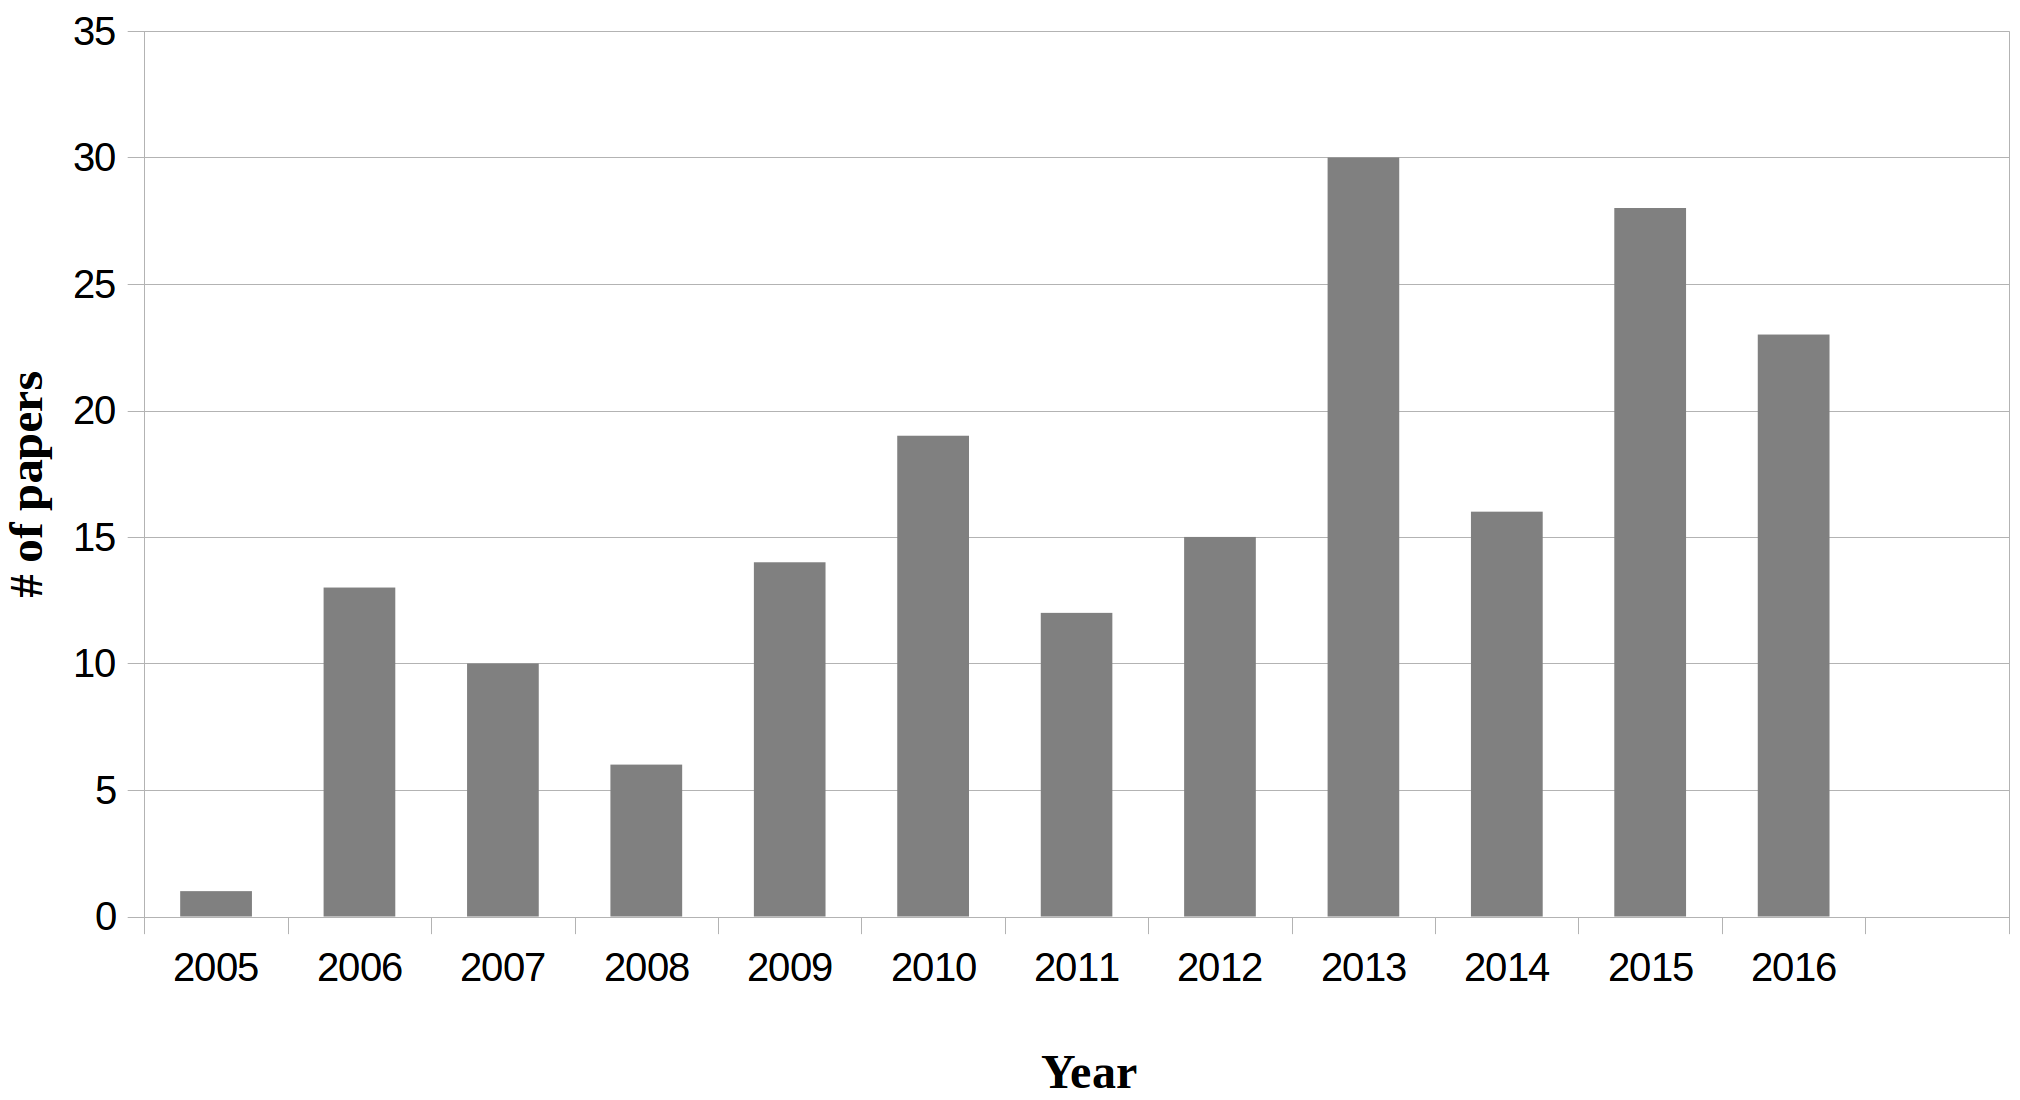
\includegraphics[width=\columnwidth]{img/evolveSZZ.png}
\caption{Sum of the number of publications using the (complete) SZZ, SZZ-1 or SZZ-2 by year of publication (N=187).}
\label{fig:evolveSZZ}       % Give a unique label
\end{figure}

Table~\ref{tableMedia} shows the different types of venues with publications where SZZ has been used. We have classified the venues in four different categories: university theses, workshop papers, conference and symposium publications, and journal articles.
Master theses, student research competitions and technical reports have been grouped under \emph{university theses}.
Diversity and maturity can be found in the sample, as it can be seen from the number of different venues (second column in Table~\ref{tableMedia}) and the considerable number of journal publications (third column in Table~\ref{tableMedia}).

%\alex{Refer to core rankings to justify why you believe MSR, ICSE, ICSME etc to be good conferences. At the same time you can argue .... the impact of SZZ is limited to people conducting empirical studies  ....... }\gema{Almost done}
\begin{table}
% increase table row spacing, adjust to taste
\renewcommand{\arraystretch}{0.8}
% if using array.sty, it might be a good idea to tweak the value of
%\extrarowheight as needed to properly center the text within the cells
\caption{ Most frequent types of publications using (the complete) SZZ (N=187). \emph{\# different} counts the different venues, \emph{\# publications} counts the total number of publications in that type of venues.}
\label{tableMedia}
\centering
% Some packages, such as MDW tools, offer better commands for making tables
%% than the plain LaTeX2e tabular which is used here.
\begin{adjustbox}{max width=\textwidth}
\begin{tabular}{|l|r|r|}
\hline
Type & \# different & \# publications  \\
\hline
\hline
 Journals & 21 & 42\\
\hline
 Conferences \& Symposiums & 40 & 102\\
\hline
Workshops & 13 & 13\\
\hline
University theses & 20 & 30 \\
\hline
\end{tabular}
\end{adjustbox}
\end{table}

Table~\ref{tableConferences} offers further insight into venues that have published more studies that use SZZ. The most frequent is the conference where SZZ itself was presented, the Working Conference on Mining Software Repositories (MSR). Two top conferences, such as the International Conference on Software Maintenance and Evolution (ICSME) and the International Conference of Software Engineering (ICSE), are second and third. SZZ can also been frequently found in high quality journals, such as Empirical Software Engineering (EmSE) and Transactions on Software Engineering (TSE).
The quality rating of conferences given in Table~\ref{tableConferences} has been obtained from the GII-GRIN-SCIE (GGS) Conference Rating\footnote{http://gii-grin-scie-rating.scie.es/}; Class 1 (CORE A*) conferences are considered \emph{excellent, top notch events} (top 2\% of all events), while Class 2 (CORE A) are \emph{very good events} (given by the next top 5\%). For journals, we offer the quartile as given by the well-known Journal Citation Reports (JCR) by Clarivate Analytics (previously Thomson Reuters).

\begin{table}[!t]
% increase table row spacing, adjust to taste
\renewcommand{\arraystretch}{0.8}
% if using array.sty, it might be a good idea to tweak the value of
%\extrarowheight as needed to properly center the text within the cells
\caption{Most popular media with publications using SZZ, SZZ-1 and SZZ-2 (N=187). ``J" stands for journal and ``C" for conference/symposium.}
\label{tableConferences}
\centering
% Some packages, such as MDW tools, offer better commands for making tables
%% than the plain LaTeX2e tabular which is used here.
\begin{adjustbox}{max width=\textwidth}
\begin{tabular}{|c|p{7.6cm}|c|c|}
\hline
Type & Name & Rating & \# papers)  \\
\hline
\hline
C & Conf Mining Softw Repositories (MSR) & Class 2 - CORE A & 15 (8\%) \\
\hline
C & Intl Conf Software Eng (ICSE)& Class 1 - CORE A* & 12 (6\%) \\
\hline
C & Intl Conf Soft Maintenance (ICSME) & Class 2 - CORE A & 10 (5\%) \\
\hline
J& Empirical Software Eng (EmSE) & JCR Q1 & 9 (5\%) \\
\hline
J & Transactions on Software Eng (TSE) & JCR Q1 & 9 (5\%) \\
\hline
C & Intl Symp Emp Soft Eng \& Measurement (ESEM) & Class 2 - CORE A & 8 (4\%)\\
\hline
C & Intl Conf Automated Softw Eng (ASE)& Class 2 - CORE A& 7 (4\%) \\
\hline
C &  Symp Foundations of Software Eng (FSE) & Class 1 - CORE A* & 6 (3\%) \\
\hline
\end{tabular}
\end{adjustbox}
\end{table}


The impact of the SZZ algorithm is significant: 458 publications cite SZZ, SZZ-1 or SZZ-2; 187 of these use the complete algorithm. The popularity and use of SZZ has risen quickly from its publication in 2005 and it can be found in all types of venues (high \emph{diversity}), ranging from top journals to workshops and PhD theses; SZZ related publications have often been published in high quality conferences and top journals (high \emph{maturity}).



\subsubsection{Are studies that use SZZ reproducible?}
Table~\ref{tableReplication} shows the number of analyzed studies that a) offer a replication package or b) have carefully detailed the methodology and the data used to allow the reproducibility of their studies. We have classified the publications in four groups: i) publications that offer a replication package (\emph{Package}), ii) publications that detail the methodology and data used (\emph{Environment}), iii) publications that have both (\emph{Both}), and iv) none (\emph{None}).

From the 187 analyzed publications, 43 offer a replication package, and 96 carefully detail the steps followed and the data used. Furthermore, only 24 provide both the replication package and the detailed methodology and data. 72 of the papers do not offer a replication package or a detailed description of the methodology and data.

\begin{table}[!t]
% increase table row spacing, adjust to taste
\renewcommand{\arraystretch}{0.8}
% if using array.sty, it might be a good idea to tweak the value of
%\extrarowheight as needed to properly center the text within the cells
\caption{Publications by their reproducibility: Rows: \emph{Yes} means the number of papers that fulfill each column, whereas the complement is \emph{No}. Columns: \emph{Package} is when they offer a replication package, \emph{Environment} when they provide a detailed methodology and dataset. Note that \emph{Both} is the intersection of \emph{Package} and \emph{Environment}. (N=187)}
\label{tableReplication}
\centering
% Some packages, such as MDW tools, offer better commands for making tables
%% than the plain LaTeX2e tabular which is used here.
\begin{tabular}{|c|c|c|c|c|}
\hline
    & Package Only & Environment Only & Both & None \\
\hline
\hline
Yes & 19 & 72 & 24 & 72 \\
\hline
No & 168 & 96 & 163 & 115 \\
\hline
\end{tabular}
\end{table}

Only 13\% of the publications using any of the variants of SZZ provide a replication package and carefully describe each step to make reproduction feasible. 39\% of the papers do not provide replication package or a detailed description of each step, making their reproduction very unlikely.

%%%%%Results of Question 3 %%%%%%%%
\subsubsection{Do the publications mention the limitations of SZZ?:}
We have classified publications into four groups, depending on how they address limitations in SZZ as a threat to validity (\emph{TTV}). Thus, we have publications that i) mention limitations of the complete algorithm (\emph{Complete-TTV}), ii) mention only limitations in the first part (\emph{TTV-1\textsuperscript{st}}), ii) mention only limitations in the second part (\emph{TTV-2\textsuperscript{nd}}), and iv) do not mention limitations at all (\emph{No-TTV}).

Table~\ref{tableTTV} offers the results of the analysis. From the 187 publications, only 39 mention limitations of the complete SZZ as a threat to validity, whereas 83 refer to limitations in the first part, and 49 only mention it for the second part. The rest, 94 studies, do not mention any limitation.

In a more profound review, we found 82 publications where a manual inspection had been done to assess these limitations: 33 of them referred to issues related to the first part of the SZZ algorithm, while 30 analyzed aspects from the second part (i.e., the bug introducing changes).
In the remaining 19 papers, the manual validation of results did not focus on outputs of the SZZ algorithm.

\begin{table}[!t]
% increase table row spacing, adjust to taste
\renewcommand{\arraystretch}{0.8}
% if using array.sty, it might be a good idea to tweak the value of
%\extrarowheight as needed to properly center the text within the cells
\caption{Number of publications that mention limitations of SZZ in their Threats To Validity (TTV). Mentions can be to the first (TTV-1\textsuperscript{st}), second (TTV-2\textsuperscript{nd}) or both parts (Complete-TTV). The absence of mentions is classified as No-TTV. Note that \emph{Complete-TTV} is the intersection of \emph{TTV-1} and \emph{TTV-2}.}
\label{tableTTV}
\centering
% Some packages, such as MDW tools, offer better commands for making tables
%% than the plain LaTeX2e tabular which is used here.
\begin{tabular}{|c|c|c|c|c|}
\hline
& No-TTV & TTV-1\textsuperscript{st} only & TTV-2\textsuperscript{nd} only & Complete-TTV \\
\hline
\hline
Yes & 94 & 44 & 10 & 39 \\
\hline
No & 93 & 143 & 177 & 148 \\
\hline
%\hline
%Total & 187 & 187 & 187 & 187 \\
%\hline
\end{tabular}
\end{table}

 Almost half (49.7\%) of the analyzed publications mention limitations in the first or second part of SZZ as a threat to validity. Limitations to the first part are reported more often than to the second part.

%%%%%Results of Question 4 %%%%%%%%
\subsubsection{Do the publications mention the limitations of SZZ?:}

It is difficult to determine which improvement has been used when the authors do not mention it in the publication. Thus, if the authors do not explicitly specify of having used an improvement, we assume that they use the \emph{original} version of SZZ. The publications are classified into one of the following groups, depending on the kind of improvement they used:

\begin{itemize}
	\item \emph{original SZZ}: Those only citing the original version and not mentioning improvements. 
	\item \emph{SZZ-1}: Those citing the improved version of Kim~\textit{et al.}~\cite{kim2006automatic}. 
	\item \emph{SZZ-2}: Those citing the improved version of Williams and Spacco~\cite{williams2008szz}.
	\item \emph{SZZ-mod}: Those citing the original SZZ with some (own) modification (by the authors). Publications in this group contain statements like ``we adapt SZZ'', ``the approach is similar to SZZ' or ``the approach is based on SZZ'', but do not refer explicitly to SZZ-1 or SZZ-2.
\end{itemize}


%\gema{A editor says: In Table 13 it is there is clearly some overlap among counts in the categories but it is not clear where it occurs. The authors will need to work out the minimum number of non-overlapping but I would imagine they should be something like Original SZZ only, SZZ plus modifications, SZZ1 only, SZZ2 only. I am not sure whether SZZ1 \& SZZ2 can be used together (even if they can it would probably be a very small category). An alternative would be to have one category for the two enhancements that includes papers that only used one of the enhancements AND papers that used both.} \gema{SZZ-1 and SZZ-2 can be used in the same paper in the sense that the paper is comparing the performance of both algorithm ~\cite{da2016framework}}
Table~\ref{tableSZZimproved} shows how many publications have used improvements to SZZ to mitigate the limitations of the original SZZ. The largest groups correspond to publications where authors use their own enhancements/adaptations (40\%) and the original SZZ algorithm (38\%). This suggests that researchers prefer to address the limitations of SZZ themselves instead of using enhancements proposed by others. Notice that the ``Mixed" column in Table~\ref{tableSZZimproved} refers to papers that have used either the original version, the improved versions or some adaptations of SZZ in the same study (e.g., to compare their performance in the same case study).
\begin{table}[!t]
% increase table row spacing, adjust to taste
\renewcommand{\arraystretch}{0.8}
\begin{minipage}{\textwidth} 

% if using array.sty, it might be a good idea to tweak the value of
%\extrarowheight as needed to properly center the text within the cells
\caption{Number of papers that have used the original SZZ, the improved versions of SZZ or some adaptations to mitigate the threat.}
\label{tableSZZimproved}
\centering
% Some packages, such as MDW tools, offer better commands for making tables
%% than the plain LaTeX2e tabular which is used here.
\begin{tabular}{|c|c|c|c|c|}
\hline
  & Original SZZ only & SZZ-improved only & SZZ-mod only & Mixed  \\
\hline
\hline
%\# publications &  63 (36\%) & 25 (14\%) &  8 (5\%) &  96 (55\%) \\
\# publications &  71 (38\%) & 26 (14\%)~\footnote{22 (12\%) of the papers use SZZ-1 and only 4 (2\%) of the papers use SZZ-2.} &  75 (40\%)  & 15 (8\%) \\
\hline
\end{tabular}
\end{minipage}
\end{table}

%Purposes of studying at the line level 
%The main question now is: why is this useful?. In most of the cases, the diff tool provides extra information about a specific commit. However, researchers have worked with the granularity of commit or a file. And there are few works using the granularity of a line.
%As specified by [Canfora et al., 2007], these studies could be used for different purposes:
%? Software evolution studies: there are plenty of studies based on the software evolution of several systems, however, with this granularity, it is possible to go a step ahead, knowing the real authorship of those lines, what could provide extra information in the terms of knowledge of the source code.
%? Effort estimation: given a specific commit, it is easy to know, how many lines have been added, removed or modified by the author of that commit. In terms of the effort estimation, this provides extra information and could be used, for instance, to create effort estimation models in FLOSS ecosystems.
%? Crosscutting concerns evolution: this item is related to the idea of how much has evolved a piece of source code. This is also interesting from the patch application point of view, checking how the patches deal with that piece of source code. In any case, a concern is a general idea, so almost any field of the software evolution field could be taken into account and improved with this approach.
%? Clones evolution: this type of studies also provide specific information of the lines that were copied or moved from one file to another one. This would help to estimate the commit when the clone was undertaken.

%In addition, other pieces of information have been identified that could help in the aforementioned purposes of study. Since, the Mozilla Foundation is using a distributed SCM, other attributes are also studied and can help:
%? Real Authorship: the use of distributed SCMs provides extra pieces of information that can be mined and later studied. This is the case of the differentiation made between author and committer in Git repositories. Or the direct use of author instead of committer in the case of Mercurial repositories. However, older SCMs such as CVS or SVN do not offer this type of information. In this case, developers interested in participating in the community need to create a patch with the changes. Those changes will be later uploaded to the server.

%As mentioned, communities tend to follow the onion model and the total work is not only done by the core developers, but also by people around the communities [Crowston & Howison, 2005]. The authorship of those sporadic changes to the source code are, in the case of distributed SCMs, registered. In other cases, like in CVS or SVN, this information, if provided, is found in the log message left by the committer or in the copyright or AUTHORS files.
%This type of information is quite useful when estimating real efforts since the effect of gatekeeper is avoided. Being a gatekeeper those developers that commit changes to the source code in behalf of others that do not have commit rights.
%? Time of commit: the use of distributed SCMs help to easily create branches and clones of the source code. Besides the registered real authorship of the changes, the time of commit (and time zone) is also registered at the moment of submitting changes to the SCM. On the contrary, centralized SCMs only keep the time of commit registered in the server. Thus, extra information related to the timezone of the developer or the actual local time of commit is totally lost.
%This type of information is quite useful when estimating time of work of the developers and type of effort that usually carried out FLOSS communities. As an example, it is possible to determine if the effort is usually undertaken during morning, afternoon or evening timeframes.



% \section{Applications}
% \label{subsec:applications}
%
% The SZZ algorithm (and its \emph{successors}) have had a considerable impact in the research community. Noteworthy is the fact that the paper with original the SZZ algorithm~\cite{sliwerski2005changes} has been cited, according to Google Scholar, 593 times as of November 2017. The enhanced version of the SZZ algorithm~\cite{kim2006automatic} based on the use of the \emph{annotation graph}~\cite{zimmermann2006mining} counts with 174 citations. Hence, there is a myriad of articles that use such algorithm in an ample number of scenarios. Without trying to be exhaustive, we offer several examples.
%
% \textbf{Bug Detection:}
% Yang \emph{et al.} apply SZZ to find what kind of bug-inducing changes are likely to become a great threat after being marked as bug-fixing changes~\cite{yangbug}. Kim \emph{et al.} show how to classify file changes as buggy or clean using change information features and source code terms~\cite{kim2008classifying}. Yin \emph{et al.} use SZZ to find how many fixes to bugs introduce new bugs~\cite{yin2011fixes}. Tantithamthavorn \emph{et al.} employ it to quickly identify the location of a bug~\cite{tantithamthavorn2013mining}.
%
% \textbf{Bug Prediction:}
% %Zimmermann \emph{et al.} have used this algorithm in order to .... developed the ROSE prototype in order to predict locations that will be changed ~\cite{zimmermann2005mining}.
%  Nagapan \emph{et al.} used the SZZ idea of mapping as the base to associate metrics with post-release defects, and they built a regression models to predict the likelihood of post-release defects for new entities~\cite{nagappan2006mining}. Zimmermann \emph{et al.}, also made use of the SZZ for predicting bugs in large software systems~\cite{zimmermann2007predicting}. Tan \emph{et al.} use it to predict whether a change is buggy at the time of a commit, evaluating the change classification techniques to address the incorrect evaluation presented by cross-validation~\cite{tan2015online}. Bettenburg \emph{et al.} apply it in the study of statistical models to predict in which parts of a software system future defects are likely to occur. Their findings showed that social information does not substitute, but rather augments traditional source code-based metrics used in defect prediction models~\cite{bettenburg2013studying}.
%
% \textbf{Software maintenance:}
% %Kamei \emph{et al.} apply this algorithm to validate effort-aware bug-prediction models~\cite{kamei2010revisiting}. Eyolfson use the SZZ to study if time of the day and developer experience affect the probability of a commit to introduce a bug~\cite{eyolfson2011time}~\cite{eyolfson2014correlations}. Izquierdo \emph{et al.} use the SZZ algorithm to see if developers are fixing their own bugs~\cite{izquierdo2011developers}. Fejzer \emph{et al.} use it to support code review~\cite{fejzer2015supporting}. %Asaduzzaman \emph{et al.} apply the SZZ algorithm on Android to study its maintainability~\cite{asaduzzaman2012bug}. Lin Tan \emph{et al.} use it to manually study bugs in three dimension ??root causes, impacts, and components. Their findings include three relevant results: (1) semantic bugs are the dominant root cause, (2) the Linux kernel operating system (OS) has higher concurrency bugs than others; and (3) reported security bugs are increasing, and the majority of them are caused by semantic bugs~\cite{tan2014bug}.
% \gema{La gente no usa las ultimas versiones}

%\section{New Nomenclature}
%\label{subsec:nomenclature}
%
%In our study, we have found that a unique terminology to name each of the concepts of the SZZ algorithm does not exist. Table~\ref{tableComparison} offers a comparison of the terminology proposed in this paper and how these concepts have been referred to in previous publications. As can be seen, we think that a common terminology when using SZZ is needed. To the best of our knowledge, no previous research has presented a comprehensive list of all the concepts and terms used and has compared if they are being used consistently.
%\begin{table}
%\newcommand{\specialcell}[2][c]{%
%  \begin{tabular}[#1]{@{}c@{}}#2\end{tabular}}
%% increase table row spacing, adjust to taste
%\renewcommand{\arraystretch}{1.3}
%% if using array.sty, it might be a good idea to tweak the value of
%%\extrarowheight as needed to properly center the text within the cells
%\caption{Comparison of our terminology with the one found in the research literature.}
%\label{tableComparison}
%\centering
%% Some packages, such as MDW tools, offer better commands for making tables
%%% than the plain LaTeX2e tabular which is used here.
%\begin{tabular}{|c|c|c| }
%\hline
%Proposed Terminology & Found as... & References \\
%\hline
%Commit & \specialcell{Change\\Commit\\Revision\\Transaction} & \specialcell{\cite{da2016framework}\cite{kim2006automatic}\\\cite{izquierdo2011developers}\cite{steff2012characterizing}\cite{izquierdo2012more}\\\cite{kim2008classifying}\\\cite{sliwerski2005changes}\cite{bettenburg2013studying}\cite{kim2006properties}}\\
%\hline
%Previous commit & \specialcell{Earlier change\\Change immediately prior\\Last Change\\Previous commit\\Recent version\\Preceding Revision} & \specialcell{\cite{sliwerski2005changes}\\\cite{williams2008szz}\\\cite{da2016framework}\cite{cao2015investigating}\cite{bavota2015four}\\\cite{izquierdo2011developers}\\\cite{kim2008classifying}\\\cite{hata2010fault}\cite{rahman2011bugcache}\cite{guerrouj2015investigating}} \\
%\hline
%Fixing Commit & \specialcell{Fix for a bug\\Bug-fixing change\\Fixed revision } & \specialcell{\cite{sliwerski2005changes}\\\cite{da2016framework}\cite{kim2006automatic}\cite{williams2008szz}\cite{izquierdo2011developers}\cite{kim2008classifying}\\\cite{hata2010fault}\cite{pan2009toward}} \\
%\hline
%Ancestral commit & \specialcell{Revision\\Change\\Commit History} & \specialcell{\cite{sliwerski2005changes}\cite{da2016framework}\cite{kim2006automatic}\\\cite{kim2008classifying}\\\cite{meneely2013patch}}\\
%\hline
%Bug introducing change & \specialcell{Fix-inducing changes\\Bug-introducing change \\defect-inducing} & \specialcell{\cite{sliwerski2005changes}\cite{williams2008szz}\cite{izquierdo2012more}\\\cite{da2016framework}\cite{kim2006automatic}\cite{kim2008classifying}\\\cite{syer2015replicating}} \\
%\hline
%\end{tabular}
%\end{table}
%
%Thus, we define as:
%
%\paragraph{Commit} It refers to any change in the code of the software.
%\paragraph{Previous commit} It refers to the immediately previous commit to the lines modified by a commit.
%\paragraph{Fixing Commit} It refers to the commit that introduces, deletes or modifies the lines to fix the bug.
%\paragraph{Ancestral commit} It refers to any early commit in the chain of modification commits of a line.
%\paragraph{Bug introducing change} It is the commit that introduces a bug in the source code.
%
%Figure~\ref{fig:example} shows a simple example to understand these concepts. Notice that boxes [1-6] are all the  changes done to a file that contains a single line of code. The bug was introduced in change \#2 and fixed afterwards in change \#5. The grey boxes correspond to non-buggy changes to the line, whereas the black ones mean that there is a bug in the line. According to our terminology, changes \#1 to \#6 are commits, where change \#5 is the \emph{fixing commit} and change \#2 is the \emph{bug introducing commit} (BIC). Furthermore, change \#4 is the \emph{previous commit} of that line and changes \#1, \#2,\#3 and \#4 are the \emph{ancestral commits}.
%
%\begin{figure}
%\centering
%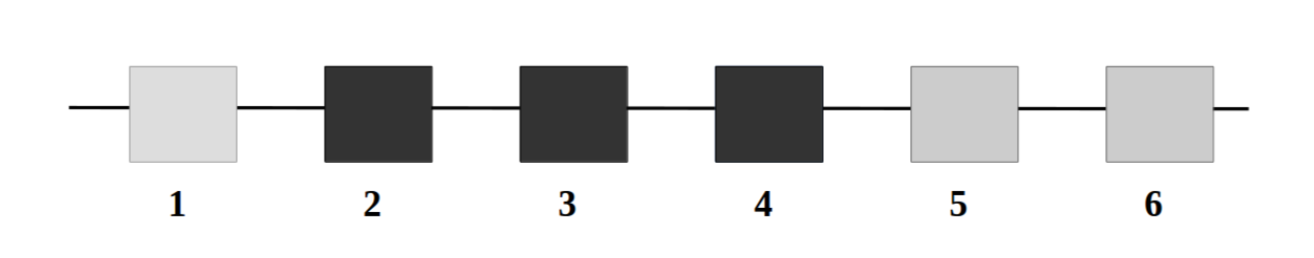
\includegraphics[width=\columnwidth]{img/example.png}
%\caption{Example of six changes done to a line to clarify the proposed, unifying terminology of SZZ concepts.}
%\label{fig:example}       % Give a unique label
%\end{figure}
%
%
%\vspace{0.2cm}
%\fbox{\begin{minipage}{30em}
%\textbf{SZZ-related terminology differs from paper to paper, making it difficult to understand, and introducing confusion. Therefore we have identified the independent concepts in SZZ (following five: commit, previous commit, fixing commit, ancestral commit and bug introducing change) and propose a clear, unequivocal definition.}
%\end{minipage}}
%\vspace{0.1cm}
%


%%%%%%%%%%%%%%%%%%%%%%%%%%%%%%%%%%%%%%%%%%%%%%%%%%%%%%%%%%%%%%%%%%%%%%%%%%%%%%%%
%%%%%%%%%%%%%%%%%%%%%%%%%%%%%%%%%%%%%%%%%%%%%%%%%%%%%%%%%%%%%%%%%%%%%%%%%%%%%%%%
% THEORY %
%%%%%%%%%%%%%%%%%%%%%%%%%%%%%%%%%%%%%%%%%%%%%%%%%%%%%%%%%%%%%%%%%%%%%%%%%%%%%%%%

\cleardoublepage
\chapter{The Theory of Bug Introduction}
\label{chap:Theory}

The proper understanding of the bug introduction process is an essential part of any research work related to the identification of the seed of a bug. The study of the changes in a bug-fixing commit to locate the origin of a bug is the foundation for researchers to carry out research studies in other disciplines of Software Engineering. For example, researchers need to identify where previous bugs were inserted and obtain their characteristics in order to build models that can predict future bugs. Also, researchers should define and understand what a bug is and how it was introduced into the source code before building classification models. To detect bugs, researchers should develop algorithms based on the learning from previous bugs patterns. However, to identify the bug-introducing change researchers rely on a common practice that only analyzes static metadata retrieved from previous changes to the modified lines in a bug-fixing commit (i.e, developer experience, lines of code inserted, type of changes, etc.). When in fact, it is necessary to keep in mind that the software evolves. It is continuously evolving thereby, a clean code today may start to become buggy tomorrow due to the dependencies and requirements of the software. There could be instances where other changes in the code or third-parties are affecting the lines, thus understanding the introduction of bugs from a static point of view may lead to problems in the results. It us therefore logical to think that a more in-depth knowledge of when and how a bug is inserted will make the state-of-the-art techniques vary in accuracy accurate. %many approaches are built upon the assumption that ``a given bug was introduced by the lines of code that were modified to fix it", or variations of it. 

There are two primary moments that should be understood and distinguished when analyzing the origin of a bug. The bug manifestation moment and the bug introduction moment; they are different but currently there is no clear distinction between them in the software research literature on bugs. The limited knowledge of when a bug is inserted into the source code makes it difficult to distinguish between these moments, and as a consequence, researchers cannot be sure whether the line(s) identified after applying these approaches inserted the bug in the same moment of inserting the lines, or if the line only manifested the bug because of other reasons. Furthermore, the lack of a meaningful model to validate these algorithms as well as the lack of definition of what needs to validated prevents researchers from calculating what a false positive or true positive is as they unsure if the line was buggy or clean at the moment of their insertion.

%there is little empirical evidence supporting it. But a careful examination surfaces many other possible sources for the introduction of bugs, from previous modifications to those lines, to changes completely external to the piece of code being considered.
With the intention of better understanding the complex phenomenon of bug introduction and bug fixing, in this chapter we carefully explain the necessity of distinguishing how bugs are introduced and how they manifest in software projects. Furthermore, we include the definitions and a taxonomy which help to analyze formally the process. The taxonomy helps to understand the many different ways in which a bug is introduced, and why some of the methods proposed in the literature might fail to find many of them. Finally, we define a model for what are bug-introducing commits, and how they are related to bug-fixing commits in order to show how state-of-the-art algorithms can be evaluated in a comprehensive and unequivocally way, something that is missing in the current literature.

%From this observation, we have developed a comprehensive model of how bugs are introduced, including definitions and a taxonomy which help to analyze formally the process. The taxonomy helps to understand the many different ways in which a bug is introduced, and why some of the methods proposed in the literature might fail to find many of them. The model allows as well for a better framing of the comparison of automatic methods to find bug inducting changes, which we apply to analyze some of these methods. Finally, based on this comparison, we propose some method that at least in the cases considered show better results than the classical methods described in the literature.


%\section{Bugs Taxonomy:}
%	\subsection{Semantic Errors}
%	\subsection{Concurrency Errors}
%	\subsection{Memory Errors}
%	\subsection{Environmental \& Configuration Errors}
%	\subsection{Build Errors}
%	\subsection{Compatibility Errors}
%

\section{Towards a Theoretical Model}

This section introduces the definition of a model to unequivocally identify bug-introducing commits. This model identifies a set of bug-introducing changes that corresponds to a set of bug fixing commits. This model includes precise definitions of \BFC and \BIC based on the assumption that there is a hypothetical test with the perfect test coverage that could be run indefinitely across the history of the source code. This model returns as true or false depending on whether or not the bug was present at a given specific moment. For the first time, this model contemplates different scenarios that have been largely excluded in the current literature, such as bug-fixing commits with only new additions, and the distinction between the moment of insertion and the moment of manifestation of a bug. 

The main aim of describing this model is to extend the current state-of-the-art approaches in order to ensure that the commits identified inserted the bug into the source code at some point in the project history. This model will be used as a framework to evaluate in a comprehensive way the performance of other approaches as well as to compare the effectiveness between different algorithms since the proposed model defines the \emph{``gold standard"} of which commits in a project are \BIC.  Before explaining in detail the theory of the model, some important concepts used to better understand the model are described below.%Despite of the large theoretical description of the model, we define in next sections \gema{Add reference to the sections}, in which aspects we are doing an abstraction in order to understand whether they might be mapped into something practical later.

\subsection{Definitions:}

Looking for the origin of the bug is a complex task that involves a huge variety of individual elements and sets in the search. In this way, we found the necessity of formulating a terminology which is one of the valuables parts in this paper, this terminology can be applied to the modern source code management systems. The terminology defines every element and every set of elements that take place during the analysis from the fixed code to the identification of the bug introducing change or the first failing change. To avoid confusion, next we define the concepts we are going to work with:
% \gema{Does it can be extender to all the SOurce code management systems? In the sense that, if we assume that we are ables to identify the atomic changes done by the same commiter around the same time is what we refer by commit in our terminology}

\paragraph{\textbf{Atomic change \emph{(at)}:}} An operation that applies a set of distinct changes as a single operation. In this thesis, atomic change is referred to as a one line minimum change.
\paragraph{\textbf{Previous atomic change:}} Given an atomic change $at$, we refer to $at'$ as the last modification which changed the line $l$ of a file $f$. Thus, the precedence relation between an atomic change and its previous atomic change is as follow:
\[ at' \rightarrow at\] 
\paragraph{\textbf{Commit \emph{(c)}:}} An observable change that records one or more atomic changes to the source code of a software system. These changes are generally summarized in a patch which is a set of lines that a developer adds, modifies or deletes in the source code. Commits update the current version of the tree directory.  
\paragraph{\textbf{Lines changed:}} By definition, a commit may change zero\footnote{When only new lines are added in a commit, zero lines are changed.} or more lines of code; we call these \emph{lines changed} of a commit and denote them as \LC{c}.
\paragraph{\textbf{Precedence between commits:}} Relation between the \emph{atomic changes} of a commit with their \emph{previous atomic changes} in the file $f$, where the previous commit of a commit is the unique previous atomic changes of an atomic changes set. We will refer to this precedence between commits as the \emph{previous commit (\pc)} of a commit in $f$ and denote it as:
\[ pc'(c) \rightarrow pc(c)\] 

\paragraph{\textbf{Previous commit set:}} Set that includes the different previous commits of a commit. Formally:% Also, can be described as the first generation of commits in ancestor change set (\ACS) of the genealogy tree for a given \BFC . We denote it as \PC{c_l}. Formally; 
\[ \PC{c} =  \bigcup pc'(c)\]

\paragraph{\textbf{Descendent Commit:}} Given a commit $c$ and a file $f$, a descendent commit of $c$ is any of the commits that belongs to the precedence commit chain of $c$ in $f$, we will refer it as $dc$.
\paragraph{\textbf{Descendent Commit Set:}} Set of descendent commits for a given commit; we refer to it as \DCSet{c}. Note that the \emph{previous commit set} contains only the previous commit to a commit, whereas the \emph{descendent commit set} contains all the commits that have modified, in somehow, the lines changed in $c$ during all the history of $f$.
\paragraph{\textbf{Ancestor  Commit:}} Is any of the commits before of a given commit, we will refer it as $ac$.
\paragraph{\textbf{Ancestor Commit Set:}} Set of the ancestor commits of a given commit; we refer to it as \ACSet{c}. Note that from a specific commit of the repository, the \emph{ancestor commit set} contains all the commits of that repository. 
\paragraph{\textbf{Immediately Ancestor  Commit:}} Is the commit immediately before to a given commit in the ancestor commit set, we will refer it as $iac$.
\paragraph{\textbf{Snapshot:}} It represents the entire state of the project at some point in the history. Using git as example, given a commit $c$, the corresponding snapshot would be the state of the repository after typing ``git checkout c". The evolution of the software can be understood as a sequence of snapshots, each corresponding to a commit, in the order shown by ``git log" (order of commits in the considered branch). 
\paragraph{\textbf{Bug-Fixing Commit (\BFC):}} Commit where a bug is fixed. As a fixed bug $b$ might require one or more commits to be fixed, we define the set of Fixing Commits (\BFC) of a bug $b$ as following set: \setBFC{b}. In general, we expect this set to be a singleton, i.e., a bug is fixed in a single commit, although several commits may be needed to fix a bug. Furthermore, a commit fixing some bug only exists whether it is really a bug at the moment of fixing, because to find out which commit introduced the bug, and it is necessary that it really being a bug.
\paragraph{\textbf{Bug-Fixing Snaptshot (\BFS):}} snapshot of the code corresponding to the \BFC.
\paragraph{\textbf{Test Signalling a Bug (\TSB):}} A test used to signal that a bug is present. It is defined as an hypothetical test, that could be run on any snapshot of the code, returning \emph{True} whether the test is passed, meaning that the snapshot does not contain the bug. And \emph{False} whether the test is not passed, meaning that the snapshot contains the bug. The test is known to pass in the 
\paragraph{\textbf{Test failing snapshot \emph{(T-S)}:}}  snapshot for which \TSB fails.
\paragraph{\textbf{Test passing snapshot \emph{(T+S)}:}}  snapshot for which \TSB passes.
\paragraph{\textbf{Bug-introducing snapshot (\BIS):}}  First snapshot in the longest continuous sequence of T-S, which finishes right before the \BFS. That is, there is a continuous sequence of snapshots for which the test fails, starting in the \BIS, and finishing right before the \BFS. Since the test is failing all the way from this snapshot up to the fix, we can know that the test was failing all the way in that sequence, and since this is the first snapshot with the test failing, we can say that this is the first snapshot ``with the bug present".
\paragraph{\textbf{Bug-introducing commit(\BIC):}} A specific commit corresponding to the \BIS that introduced the buggy line(s) at the moment of their insertion, and the bug propagated through each following commit until the \BFC fixed the line(s).
\paragraph{\textbf{First Failing commit (\FFC):}} The first commit corresponding to the \BIS that manifest the bug but it did not introduce the buggy line(s) at the moment of their insertion.


%\paragraph{\textbf{Atomic change:}} Represents an operation that applies a set of distinct change(s) as a single operation. In this work, we refer to an \emph{atomic change} as a one line minimum change ($at_l$), where $l$ is the label used to identify uniquely the line in a specific version of a specific file $f$.
%
%\paragraph{\textbf{Previous atomic change:}} Given an atomic change $at_l$, we refer to $at'_l$ as the last modification which changed the line $l$ of $f$. Thus, the precedence relation between an atomic change and its previous atomic change is as follow:
%\[ at'_l \rightarrow at_l\] 
%
%\paragraph{\textbf{Commit/Change:}}It is an observable change with an unique identifier in a SCM, that gathers the set of one or more atomic changes applied by the same author at the same time. We will refer to a general commit~\footnote{Notice that in this paper we use commit and change interchangeably} as $c$.
%
%\paragraph{\textbf{Lines changed:}} By definition, a commit may change zero\footnote{When only new lines are added in a commit, zero lines are changed.} or more lines of code; we call these \emph{lines changed} of a commit and denote them as \LC{c}.
%
%%\textbf{Previous commit:} It is the commit immediately before a given commit using the lineal vision. 
%\paragraph{\textbf{Precedence between commits:}} Relation between the \emph{atomic changes} of a commit with their \emph{previous atomic changes} in the file $f$, where the previous commit of a commit is the unique previous atomic changes of an atomic changes set. We will refer to this precedence between commits as the \emph{previous commit (\pc)} of a commit in $f$ and denote it as:
%\[ pc'(c) \rightarrow pc(c)\] 
%
%\paragraph{\textbf{Previous commit set:}} Set that includes the different previous commits of a commit. Formally:% Also, can be described as the first generation of commits in ancestor change set (\ACS) of the genealogy tree for a given \BFC . We denote it as \PC{c_l}. Formally; 
%\[ \PC{c} =  \bigcup pc'(c)\]
%
%\paragraph{\textbf{Descendent Commit:}} Given a commit $c$ and a file $f$, a descendent commit of $c$ is any of the commits that belongs to the precedence commit chain of $c$ in $f$, we will refer it as $dc$.
%
%\paragraph{\textbf{Descendent Commit Set:}} Set of descendent commits for a given commit; we refer to it as \DCSet{c}. Note that the \emph{previous commit set} contains only the previous commit to a commit, whereas the \emph{descendent commit set} contains all the commits that have modified, in somehow, the lines changed in $c$ during all the history of $f$.
%
%\paragraph{\textbf{Ancenstor Commit:}} Is any of the commits before of a given commit, we will refer it as $ac$.
%
%\paragraph{\textbf{Ancestor Commit Set:}} Set of the ancestor commits of a given commit; we refer to it as \ACSet{c}. Note that from a specific commit of the repository, the \emph{ancestor commit set} contains all the commits of that repository. 
%
%\paragraph{\textbf{Immediately Ancenstor Commit:}} Is the commit immediately before to a given commit in the ancestor commit set, we will refer it as $iac$.
%
%\paragraph{\textbf{Bug-Fixing Commit:}} Commit where a bug is fixed. As a fixed bug $b$ might require one or more commits to be fixed, we define the set of Fixing Commits (\BFC) of a bug $b$ as following set: \setBFC{b}. In general, we expect this set to be a singleton, i.e., a bug is fixed in a single commit, although several commits may be needed to fix a bug.
%
%\paragraph{\textbf{First Failing Change:}} The first commit of the \DCSet{c} in which the bug manifests itself in the project. We will refer to it as \FFC .
%
%\paragraph{\textbf{Bug Introducing Change:}} A specific commit from the \ACS{c} that erroneously wrote the buggy line(s) at the moment of their insertion, and the bug propagated through each following commit until the \BFC fixed the line(s).

It is to be noted that some of these terms have been used for different concepts in the literature; and from it, it can be understood why we argue that a common terminology when investigating bug fixing activity is needed. Table~\ref{tab:tableComparison} offers a comparison of the terminology proposed in this paper and how these concepts have been referred in previous works through a diverse terminology. To our knowledge, no previous research has presented a comprehensive list of all concepts needed to have a clear and complete vision of the problem. 

\begin{table*}
\centering
\newcommand{\specialcell}[2][l]{%
  \begin{tabular}[#1]{@{}l@{}}#2\end{tabular}}
% increase table row spacing, adjust to taste
\renewcommand{\arraystretch}{1.3}
\caption{Comparison of our terminology with the one found in the bug seeding field.\gema{Add the descendent commit}}
\label{tab:tableComparison}

\begin{tabular}{lll}
\toprule
\textbf{Proposed Terminology} & \textbf{Found as..} & \textbf{References} \\
\midrule
 \multirow{4}{*}{Commit} &Change & \cite{da2016framework}\cite{kim2006automatic}\\
 &Commit& \cite{izquierdo2011developers}\\
 &Revision& \cite{kim2008classifying}\\
 &Transaction & \cite{sliwerski2005changes}\cite{bettenburg2013studying}\\
\hline
\multirow{6}{*}{Previous Change} &Earlier change & \cite{sliwerski2005changes}\\
 &Change immediately prior& \cite{williams2008szz}\\
 &Ancestor commit & \cite{blondeau2017testing}\\
 &Previous commit & \cite{izquierdo2011developers}\\
 &Recent version & \cite{kim2008classifying}\\
 &Preceding version & \cite{hata2010fault}\\
 \hline
\multirow{3}{*}{Bug Fixing Change} &Fix for a bug & \cite{sliwerski2005changes}\\
 &Bug -fixing change& \cite{da2016framework}\cite{kim2006automatic}\cite{williams2008szz}\cite{izquierdo2011developers}\cite{kim2008classifying}\\
 &Fixed revision& \cite{hata2010fault}\\
 \hline
\multirow{2}{*}{Ancestor Change} &Revision & \cite{sliwerski2005changes}\cite{da2016framework}\cite{kim2006automatic}\\
 &Changes& \cite{kim2008classifying}\\
\hline
\multirow{2}{*}{Bug Introducing Change} &Fix-inducing Change & \cite{sliwerski2005changes}\cite{williams2008szz}\\
 &Bug Introducing Change& \cite{da2016framework}\cite{kim2006automatic}\cite{kim2008classifying}\\
\bottomrule
\end{tabular}
\end{table*}

%\paragraph{\textbf{Axiom 1}}: Assuming that our model present a 100\% test coverage, that we are aware of the correct behavior of the project in each moment and, that we have a perfect test that can be run forever in the past. We always are able to : (i) identify the \FFC whether it belongs to the \ACS of a bug, in the worst case, we restrige the \FFC to be in a temporary window and, (ii) identify unequivocally the \BIC (whether it exists).
%\paragraph{\textbf{Axiom 2}}:
%\paragraph{\textbf{Axiom 3}}:

\subsection{The Explanation of the Model:}
All too often when analyzing projects, researchers use \texttt{git} as their \textit{Source Code Management (SCM)} system. The SCM records \emph{observable changes} to a file or set of files. Observable changes are alterations of the file(s) caused by additions, deletions or modifications of one or more lines in the source code. Thanks to the SCM, researchers are able to manually or automatically track back the deletion and modification of lines from a specific moment up until its origin, they are also able to identify which lines are new additions in each commit. Navigating back into the relationship between the altered lines of each observable change and its previous one, a \emph{precedence observable change tree} or \emph{genealogy tree} can be built. Figure~\ref{fig:genealogytree} shows an example of the observable change $i$ made in a file $f$ that fixed the bug $b$. Tracking back each line modified or removed from $f$, we can draw the genealogy tree of the lines involved in $i$. It is important to notice that the new addition lines cannot be tracked, but they still remain in the model. The black boxes represent the different commits, the dots represent a hunk of only new lines, the arrows show the precedence between commits, and the colour of the lines depend on whether they are removed (red), added (green) or modified (black). 

Using the defined terminology, we will refer to the observable change $i$ as the \BFC. From the lines changed in the \BFC, \LC{\BFC}, we might draw its genealogy tree in which, thanks to the precedence between commits, there is a genealogical relationship. Visually from this relationship, we distinguish between commits of the first generation \emph{(i-1a,i-1b,i-1c)}, second generation \emph{(i-2a, i-2b, i-2c, i-2d)}, and third generation \emph{(i-3a)} of the \BFC. By extension, the Previous Commit Set of the \BFC, are the first generation commits and the Descendent Commit Set are the first, second and thrid generation of commits. 
\[ \PC{\BFC} =  {(i-1a,i-1b,i-1c)}\]
\[ \DCSet{\BFC} =  {(i-1a,i-1b,i-1c),(i-2a, i-2b, i-2c, i-2d),(i-3a)}\]

\begin{figure}[ht]
\centering
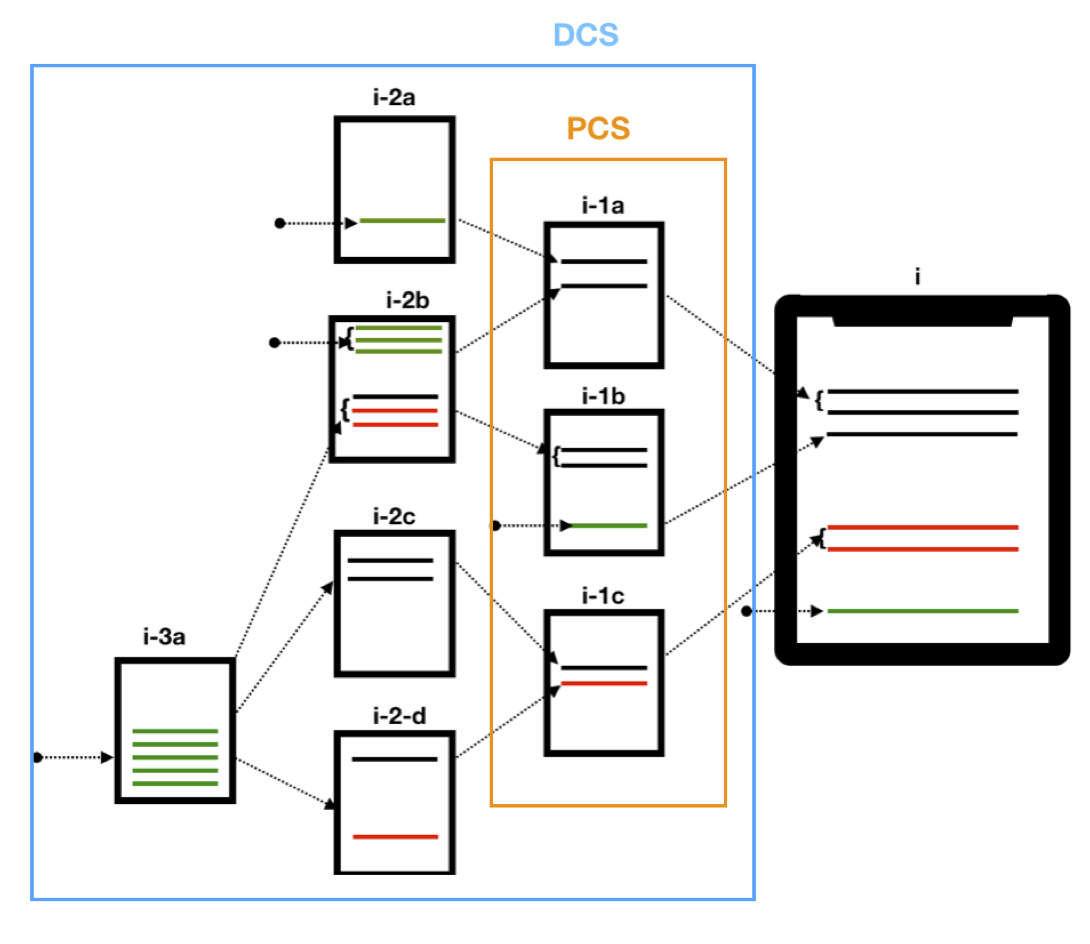
\includegraphics[width=200pt,height=200pt]{img/visiontree.png}
\caption{Genealogy tree of the observable change $i$, each commit shows a precedence relationship its descendent commits .}
\label{fig:genealogytree}       % Give a unique label
\end{figure}

%In our study we have only 
%which form a chain of precedence built by all ancestor changes of the file. Thus when flattening the genealogy tree,
When focusing on commits in the \emph{master} branch of a project repository we do not have a clear visual access to the genealogy tree of a given commit, but we have a flatten version of all the ancestor commits of a given commit. In this flattened version, the commits are preceded by other changes making up a lineal vision of precedence, where the commits of the genealogy can be found. An important concept is that this precedence is not set by dates, but by previous versions in the SCM. This occurs due to the way in which a decentralized source code management (DSCM) system works. Bird \emph{et al.} explained how the local repositories of two collaborating developers working with git might diverge, which causes that each repository to contain new commits that are not present in the other. Thus, in the moment of combining both local repositories, the user can select between many options regarding the sequence of commits such as to rebase, merge, remove, squash, etc. These actions may alter the natural order of commits, which inhibits them form being sorted in time~\cite{bird2009promises}. Continuing with the above example, Figure~\ref{fig:precedence} demonstartes the lineal vision of precedence of the change $i$ in the \emph{master} branch of a project repository. The commits are represented by circles, and the changes belonging to the genealogy tree of $i$ can be found in orange, based on whether they are a $pc$ in blue, or whether they are a $dc$; the remaining commits are the $ac$ where the commit before a $is$ is the immediately ancestor commit $iac$. The \ACS{i} were committed to the project; however, they do not have a precedence relationship with the lines modified in $i$.    

For those who are familiarized with \texttt{git}, we can compare the Figure~\ref{fig:genealogytree} with the \texttt{git blame} of the modified lines in a bug-fixing change and Figure~\ref{fig:precedence} with the \texttt{git log} of a given commit in the master branch of a project repository. 

\begin{figure}[ht]
\centering
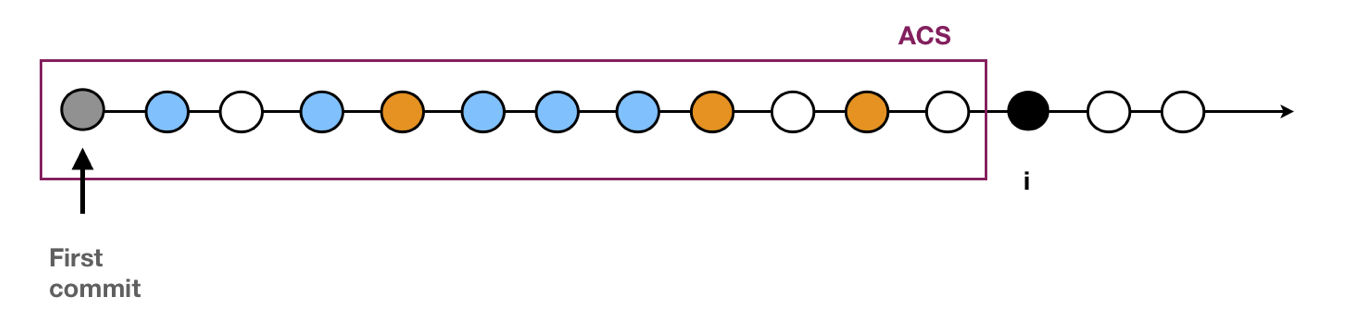
\includegraphics[width=\columnwidth]{img/visionlog.png}
\caption{Lineal vision precedence in the master branch of the bug-fixing change $i$. The coloured commits belongs to the \PC{i} (orange) and \DCS{i} (blue), the black commit is the \BFC and the grey commit is the initial commit of the project. Notice that the commits are not sort in time because we are not assuming a precedence set by dates.}
\label{fig:precedence}       % Give a unique label
\end{figure}

%\begin{figure}[ht]
%\centering
%\includegraphics[width=\columnwidth]{git.png}
%\caption{git merge, git rebase and SVN lineal history}
%\label{fig:git}       % Give a unique label
%\end{figure}

%Definicion del momento del Fallo
%When identifying a change or a set of changes in a bug-fixing commit, what we would like is to understand the genealogical relationship of the fixed lines with their ancestor lines

From an objective point of view, it is not important \emph{WHEN} the bug was inserted in time but, \emph{WHAT} commit inserted it. This is because after inserting the erroneous lines in a previous commit or an ancestor commit of a \BFC, the bug is in the system and furthermore, it propagates through each new change in the file. Hence, determining the first failing change that manifests the bug implies to navigate back into the genealogy tree. Thus, from a theoretical point of view, there will be one change in the lineal vision precedence that manifest the malfunction by first time. This change will be the first failing change, and will be referred as \FFC. Furthermore, the \FFC may be the bug introduction change based on whether it inserted the buggy line(s) and whether it belongs to the \ACSet{\BFC}; when there is no change that inserted the wrong line(s) the \BIC in the \ACSet{\BFC} cannot be found, as a result the \FFC is used to explain that in this precise commit, other (external/internal) changes that do not belong to the \ACSet{\BFC}, affected in somehow a line(s) of the source code caused the failure of the system and the bug manifestation.


%\subsection{Effectiveness of the approaches in order to find the \FFC.}

%Unfortunately, the vast majority of approaches for finding the bug introducing commit, or for predict future bugs, are not understood for the \emph{real} cause of the bug, forcing practitioners to apply these approaches to all the projects without regard the nature of the bug, the dependencies of the bug or even whether they use SVN or Git.

%Some people may ask why CVS or git is relevant when we are using the approaches to find the BIC and the explanation is that some approaches bore to be use in SVN because of the branches are explicitly created, but this is not the case with git. A branch in git is only a pointer to some commit which can  move causing that we lose the previous states completely. In other words, as we explain before git does not keep a relationship of the changes setting in time, thus the approaches that use temporally windows to remove false positives or have faith that the lineal vision precedence is setting by dates are not suitable in git. Moreover, as we have explained before, it is not fair to blame changes as the BIC when in fact they are not the real cause of the bug, so to be more accurate in the results and can learn from the history of the projects taking into account all the factors around, we have proposed to find the \FFC instead of the BIC and, furthermore we must understand that this \FFC has dependencies which help to comprehend the origin of the bug. 


\section{How to Find the Bug Introducing Change and the First Failing Change:}
In order to discover the Bug-Introducing Change with the maximum accuracy, it is recommended to do it manually by tracking back each line of the source code of all changes until find the \emph{moment} where the bug was inserted. To ensure that it is the moment when the bug was inserted, it is necessary to use information from the code review system and version control system. If according to this information, the commit inserted the line(s) contains the bug at this moment, the change is regarded as \BIC. On the contrary, if the information gathered form these systems explains that there was a change in the \emph{environment or context} that caused the failure, it is not a \BIC, and in this case the change is the First-Failing Change. 

Theoretically and under optimal conditions, this process can be fully automatic relying on the Test Signaling a Bug (\TSB) which flags as \emph{True} when the test is passed and \emph{False} when the test fails in the analyzed snapshots of the project. Despite the high complexity of automatization, there us an easy way to find the \BIC or \FFC in this model, which can be achieved through looking manually for the first snapshot when the \TSB fails. This snapshot contains the commit that is the perfect candidate to be the \BIC or the \FFC.

This model focuses on the cases when a \BIC for a BFC can be found or the cases when it is sure that a \BIC for a \BFC does not exist. To show how the model works, the definitions of \BIC and \BFC based on the existence of a \TSB are applied. The \TSB is applied in all the snapshots of the lineal vision precedence of a \BFC to identify whether there is a Bug-Introducing Commit. Considering that the \TSB  has a coverage of 100\% and that it can run indefinitely across the history of the source code, the proposed model is able to find out the \BIC or the \FFC of a bug report by analyzing the changes that fixed the bug. This \TSB will be passed into all the descendent commit set of the lines modified in the bug-fixing commit. Thus, when the \TSB test is passed to all the snapshots, it looks for the snapshot that fails; if found, the model will consider it as a candidate for the \BIC. %depending on how the \TSB fails.  %Furthermore, we will be sure if such \FFC might be the \BIC by using some heuristics that check that the line(s) inserted by this commit was (were) buggy, otherwise it cannot be considered as the $BIC$.


%For instance, a similar notion to locate the \FFC would be to use the \emph{Oracle} as a conceptual idea, which is used in testing to determine whether the result of executing a program using a test is correct~\cite{staats2011programs}. Therefore we can take this concept to find the \FFC asking to the \emph{Oracle} whether after a specific change the result of the program is correct. The oracle is only a part of specifications related to the expected output (when it exists) and, contains information about the input ranges, about non-functional properties, etc. As example, a test suite will be a specification, that contains test cases, which themselves contain assertions (oracles).



%\gema{To show the model working, we find a set of BFCs in two projects, and find out (manually) their BICs, or ensure that there is no BIC at all. For this, we apply our definitions of BIC and BFC based on the existence of a TSB, that we could declare in English (so that we can be more precise if we agree or not on which one is the BIC for a BFC). If we cannot find the BIC (or agree on it, or be sure that there is no BIC), we could consider excluding the corresponding BFC from the study, since we're focused in the cases when BIC can be found or we're sure it does not exist (we can see through an Aleph). The main contribution of this part is showing that in a real case, the ``gold standard" idea can be put in practice, at least to some extent (I hope to a large fraction of the BFCs in our dataset, but that's what we need to explore further, since the preliminary exploration didn?t work that way).}

%\gema{Given a certain BFC, the algorithm should be able of finding the corresponding BIC, or showing that no BIC exists. If a certain commit is identified as the BIC, but it is not (maybe because there is no BIC), that's a false positive. If no commit is found to be the BIC, but there is one, that's a false negative. Of course, this assumes we can see through the Aleph, and we have perfect knowledge of which one is the BIC corresponding to any BFC (if it does exist), or that it does not exist}

%\gema{I can think of several reasons: 
%The snapshot is the first snapshot when the test can be applied. Depending on how ``perfect" we consider our hypothetical test, this would be the first snapshot of the code, or the first snapshot when it is reasonable to try to apply the test (eg, when the function or feature tested starts to be present). Since our hypothetical tests are, well, hypothetical, we could just consider that we can run them all the way to the first snapshot, and maybe that is cleaner. In reality, any sensible test could be applied for the first time to a certain snapshot, and it wouldn't make sense to try to run it before that (as said above, for example before the tested function or feature is present).
%An special case is when the test fails in all the sequence up to the first snapshot with a given environment (eg, external APIs, etc.), but passes in all the sequence snapshots up to the first snapshot with a different environment (eg, the current environment). That would be an indicator of the bug being due to changes in the environment, not in the code. Of course, we need to define environment.
%}

%Figure~\ref{fig:testrecursive} naive shows how the outcomes of hypothetical test. 

\subsection{Outcome of the TSB:}
The outcome of the \TSB varies depending on each snapshot, there are three different outcomes:
\begin{enumerate}
	\item {\textbf{Pass}} : The function or feature tested is present in the snapshot and it works as the test anticipated according to the BFC, there is no \BIC.
	\item {\textbf{Fails}} : The function or feature tested is present in the snapshot but it does not work as the test anticipated according to the BFC. This snapshot is considered as candidate to be the \BIC.
	\item {\textbf{Not-Runnable}} : The function or feature tested is not present in the snapshot, thereby the test cannot run in this snapshot. 
\end{enumerate}

%\begin{figure}[ht]
%\centering
%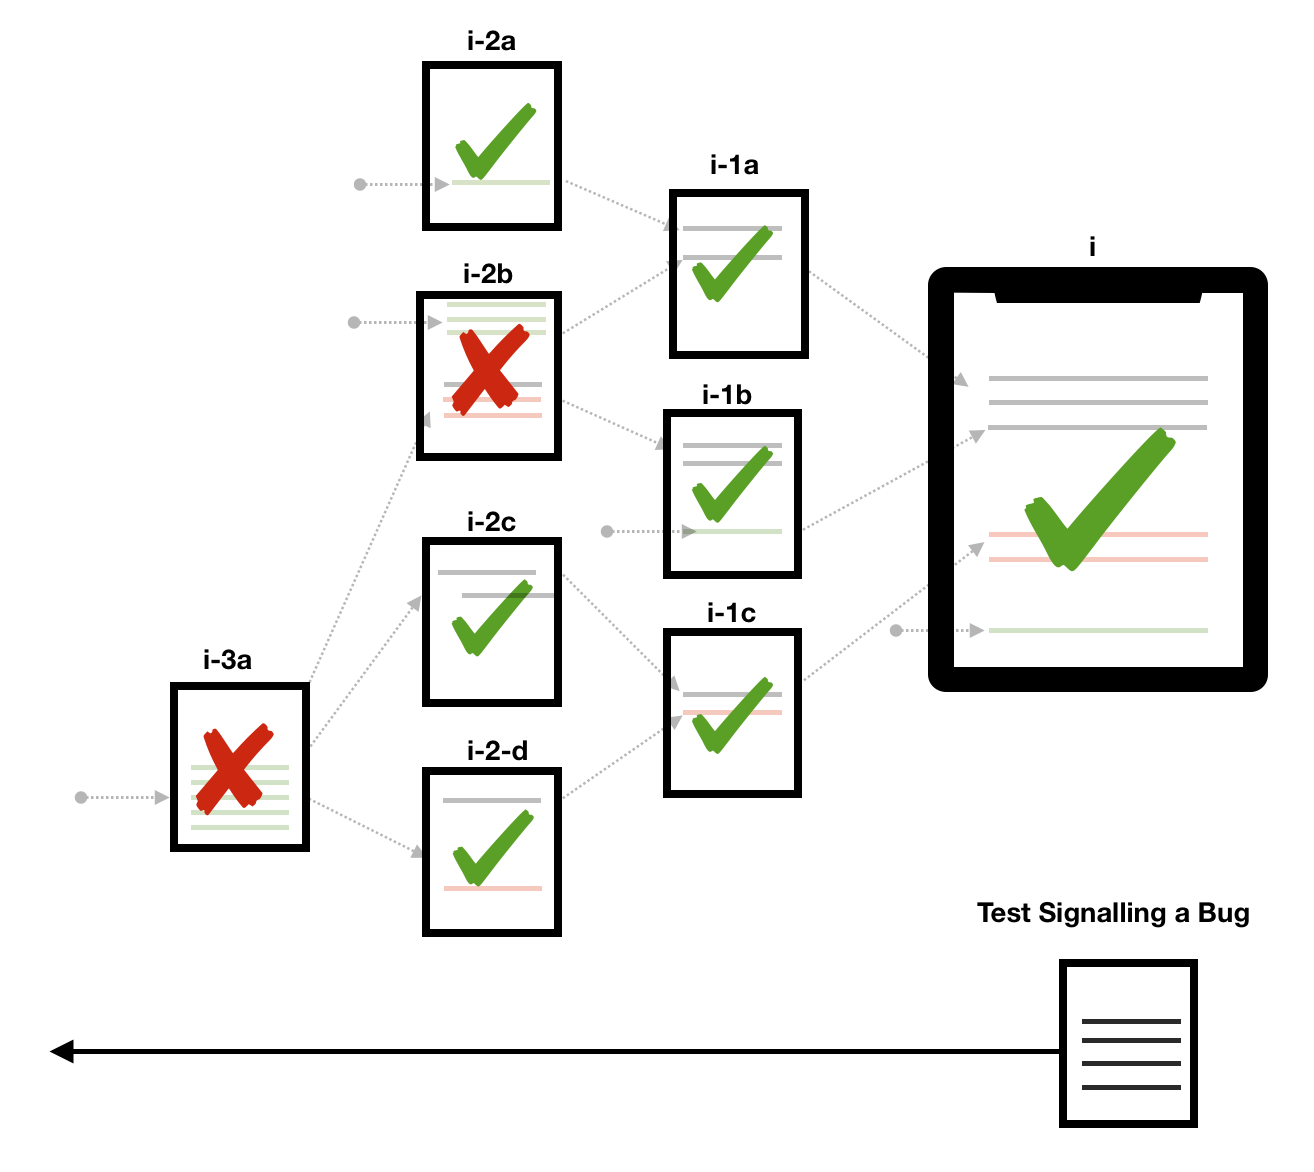
\includegraphics[width=200pt,height=170pt]{img/testrecursive.png}
%\caption{Omnipotent view of a test that automatically locates the \FFC}
%\label{fig:testrecursive}       % Give a unique label
%\end{figure}
There are three different scenarios to illustrate how to apply the hypothetical test into a lineal vision of precedence for the \setBFC{i} in order to identify whether the Bug-Introducing Commit exists. In these scenarios it is considered that the \TSB have 100\% of coverage and that it can run indefinitely across the history of the source code. Thus, the \TSB is passed to all the snapshots (ancestral commit set) in search for the one that fails; if found, it will be consider it as a candidate for the \BIC. %Furthermore, we will be sure if this snapshot is the \BIC by using some heuristics that check that the line(s) inserted by this commit was (were) buggy, otherwise it cannot be considered as the $BIC$.

Figure~\ref{fig:snapshot1} shows how to apply the hypothetical test into the genealogy tree when there is a \BIC and the \TSB can be run in all the snapshots. To locate the \BIC, the \TSB is passed into all the snapshots of the descendent commit set, and the \BIS will be the first that fails (i-1b). It can be known that the \BIS is a \BIC because the snapshot before (i-2c) passes. 

\begin{figure}[ht]
\centering
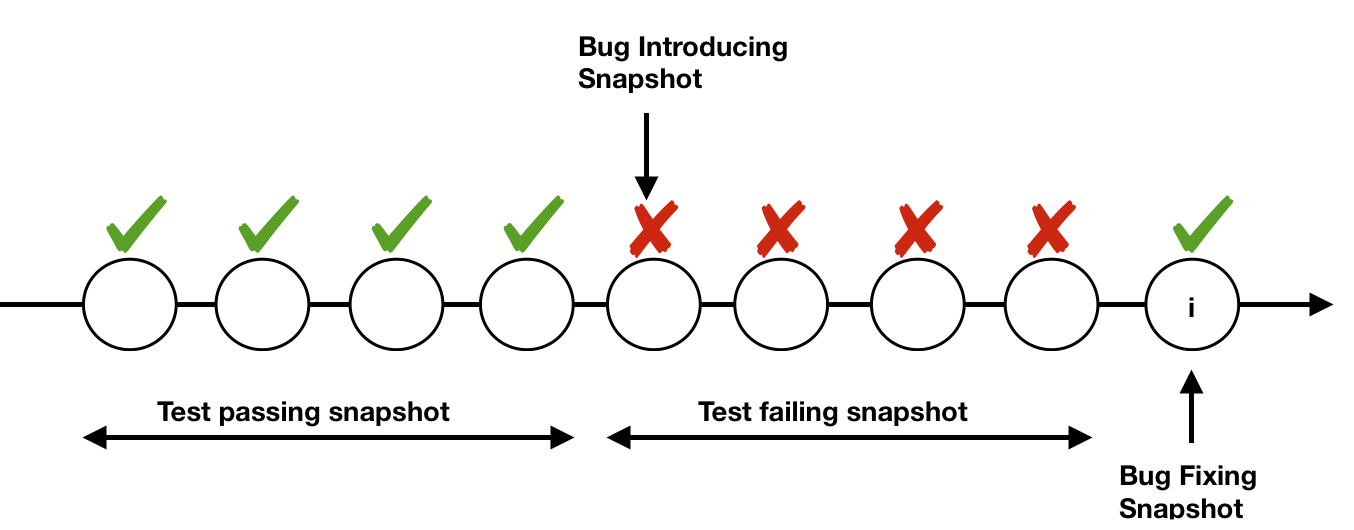
\includegraphics[width=\columnwidth]{img/snapshot1.png}
\caption{The Bug Introducing Snapshot is the \BIC}
\label{fig:snapshot1}       % Give a unique label
\end{figure}

Figure~\ref{fig:snapshot2} shows how  the hypothetical test is applied to the genealogy tree when there is a \BIC but the \TSB test cannot be run after a snapshot. This is because the tested function or feature is not present in that moment. Here, the first \BIS identified is the \BIC because when it introduced the function or feature tested, it was buggy.

\begin{figure}[ht]
\centering
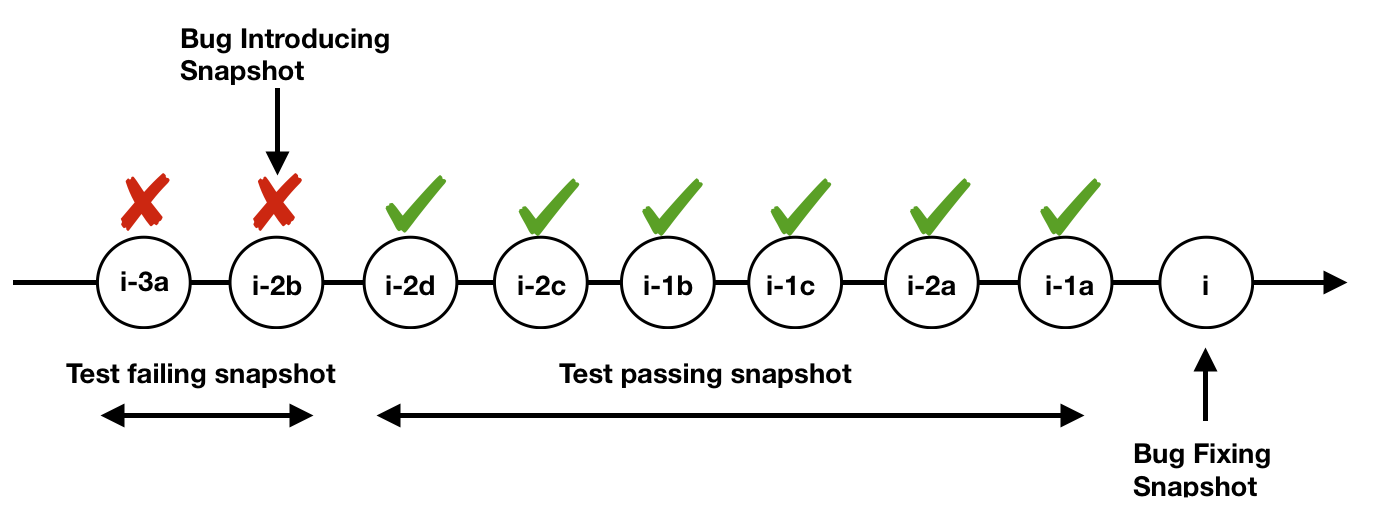
\includegraphics[width=\columnwidth]{img/snapshot2.png}
\caption{The Bug Introducing Snapshot is the the \FFC }
\label{fig:snapshot2}       % Give a unique label
\end{figure}

Figure~\ref{fig:snapshot3} 5 shows how the hypothetical test is applied to the genealogy tree when there is not BIC and the \TSB can be run indefinitely across the history of the source code. . The \TSB always fails with the BFS environment the snapshots, but if the older environment is set, it will pass in the descendent snapshot. Thus, the first \BIS before the \BFC will be the \FFC, there was not \BIC in the descendent commit set.
\begin{figure}[ht]
\centering
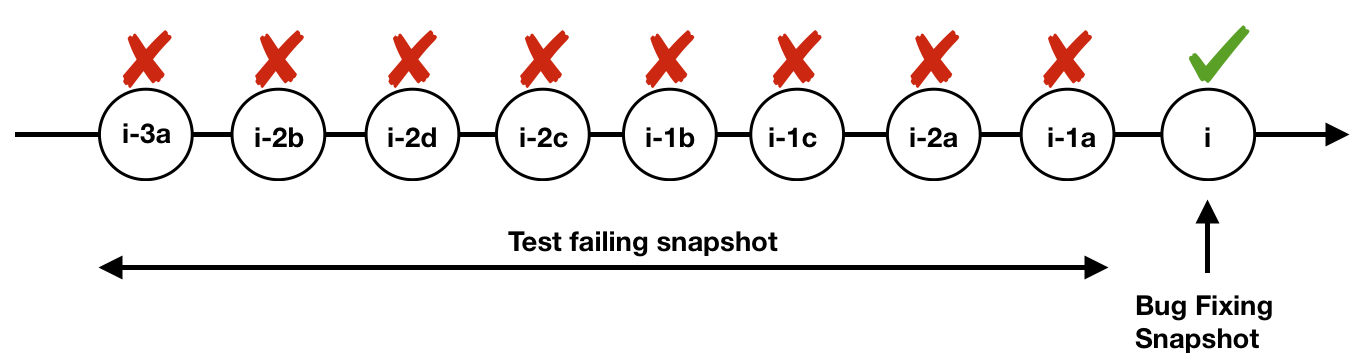
\includegraphics[width=\columnwidth]{img/snapshot3.png}
\caption{The Bug Introducing Snapshot is the the \FFC }
\label{fig:snapshot3}       % Give a unique label
\end{figure}


\subsection{Criterion to apply to the test Signalling a Bug:}
 \gema{Write some intro here. que tenemos que hacer cuando no hay una vision linear si no que tenemos branches. Decir que la idea de test se va a aplicar a todos los ancestor commits }
 \gema{Explicar porque algunas veces no encontraremos el FFC cuando tiene sentido hablar de FFC, explicar que otras veces no vamos a estar seguros ....}
 \begin{enumerate}
	\item Undecidable \FFC : When we cannot find the \FFC. In this class, we will not find the \FFC between all the \ACSet{b} using the test, because the test may not be implemented due to some factors. Thus, the \FFC will be the first change that manifests the bug in the lineal vision precedence under analysis.
	\item \FFC in external dependencies: When the bug is not caused by a change committed into the ancestral tree under analysis but, another external factors cause the failure such as: (1) There is a bug in the dependencies of the project; (2) There is a bug in API's used in the project. In this class, we will find the \FFC between all the \ACSet{b} using the test, but this \FFC is not the cause of the bug, this \FFC will be the first time that the malfunction manifests in my lineal vision precedence.
	\item \FFC : When we can find the \FFC between all the \ACSet{b} using the test and furthermore, this \FFC is the cause of the bug.
\end{enumerate}

Nevertheless, it would appear that automatizing this process is tedious and complex, because all the external dependencies used in the project makes it more complicated to build an isolated test to run in each previous change. However, we still rely this can be possible thanks to studies such as the one performed by Bowes~\emph{et al.}, which provides a core list of testing principles that focuses on different quality aspects other than effectiveness or coverage. For our research, the most interesting principle is the test (in)dependency which describes that a test should be able to run in any order and in isolation. In addition, the test should  not  rely  on other tests in anyway. Allowing practitioners to add new tests without keeping in mind dependencies or effects they might have on existing tests~\cite{bowes2017good}.

\section{Algorithm to Find the BIC and the FFC:}
Figure~\ref{fig:algoritmo} presents the decision tree in order find the \BIC, whether it exists, and the \FFC. This decision tree is implemented in our model and includes the current shortcomings in the state-of-the-art approaches based on tracking back the lines that have been modified in the \BFC in order to find the \BIC.

 \begin{enumerate}
	\item {\textbf{Lack of guidelines when SZZ identifies more than one pc}}: The decision tree can distinguish when there are more than one previous commit and what needs to be done to identify the \BIC or the \FFC.
	\item {\textbf{Only new added lines in the BFC}}: The decision tree can distinguish when there are only new lines added in the \BFC. In this case, the PC Set is computed by identifying the pc of the lines surrounding the new additions. 
	\item {\textbf{Modifications are not related with the root cause of the bug}}: The \TSB does not test the functions or features that are not related with the root cause of the bug.
	\item{\textbf{ More than one issue are addressed by the BFC}}: The \TSB only implement the test for the functions or features that caused the bug.
	\item {\textbf{Lines correct at the time of their insertion}}: The \TSB always fails with the BFS environment in the snapshots, identifying the \FFC.
	\item {\textbf{Dormant Bugs}}: The \TSB will identify the first snapshot in which the test fails, identifying the \BIC.

\end{enumerate}

\begin{figure}[ht]
\centering
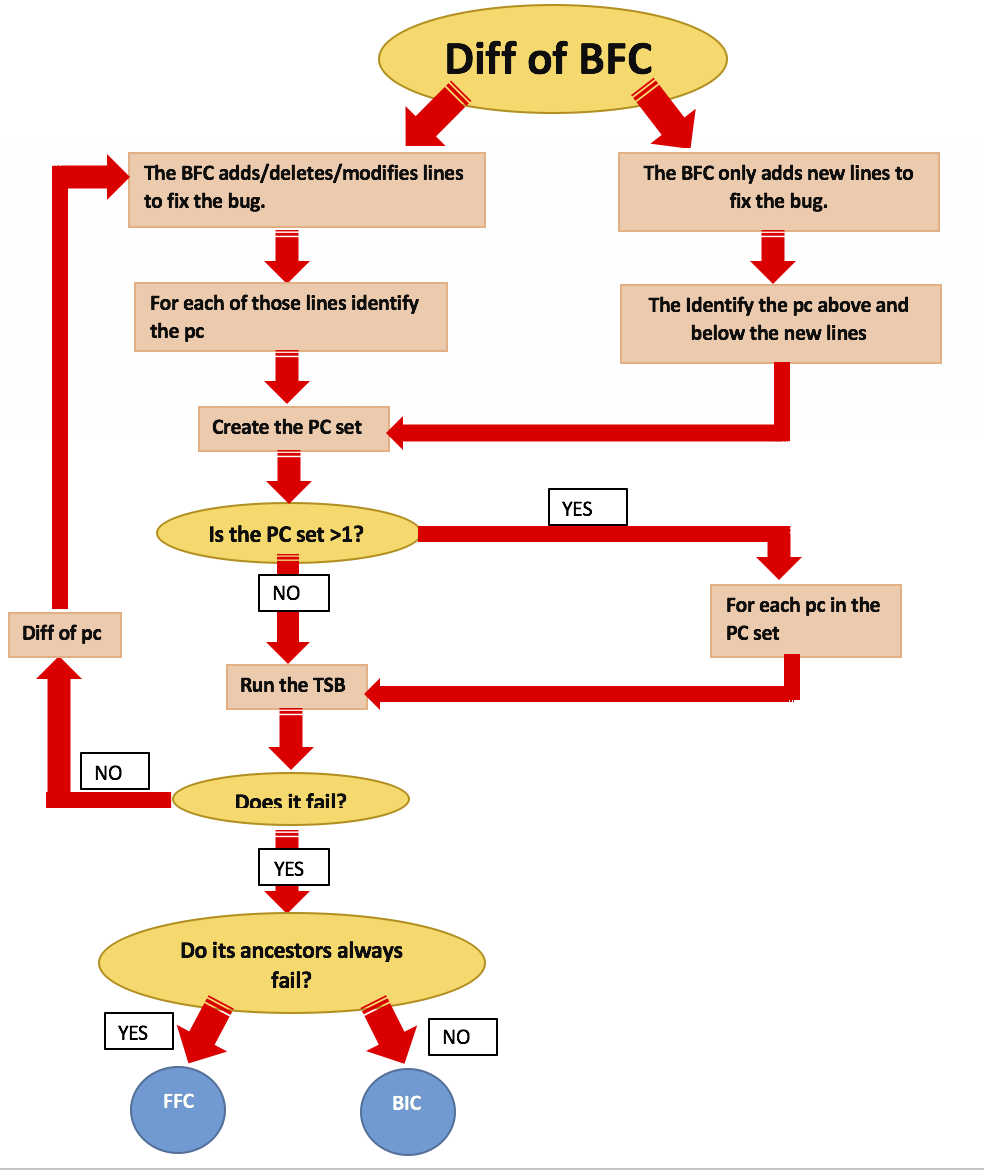
\includegraphics[width=\columnwidth]{img/algoritmo.png}
\caption{Decision tree }
\label{fig:Decision tree to identify the BIC and the FFC}       % Give a unique label
\end{figure}

%To be more precise: we consider bugs that are considered bugs at the moment of bug fixing. There is a (hypotetical) test that fails right before the commit fixing the bug, and does not fail right after the commit fixing the bug. In the case of Elasticsearch, we rely (to a great extent) in developers labelling it as bug. In the case of OpenStack, it is more that Gema did an analysis, using info that developers annotated in the bug report.

%Yes, we should exclude those bugs, because we're interested in how bugs are introduced in the code. This said, in some cases the line may be fuzzy, but I would suggest excluding cases which are not clear bugs (at least in a first round). Because if it is not cleary a bug fixed, there is (maybe) no bug introduction to look for.

% Question: What if bug fixing has been incomplete and spread over several commits (whether or not in a temporal proximity to each other?
%I think this has to do with how we define a bug. Again, if we consider the test-based definition described above, the important thing is that for each bug-fixing commit we will have a test, that will fail or not. If it happens that some fixes were not complete, the several bug-fixing commits will still point to the same bug-introducing commit (except if it was really several bugs "together", that can be addressed separately). Since our problem is how to locate those bug-introducing commits, I think that should not be a problem.

%I think this is only relevant when evaluating a certain SZZ-like algorithm. That should be discussed once we agree on our model for deciding which one is the BIC (see definitions after the text by Alexander), and how we find it in our exploratory cases.

%The task would be, in general terms:
%* Identify a certain number of BFC, being sure they are really bug-fixing.
%* For each of them, find the corresponnding BIC, or decide it does not exist
%(see definitions below).The best way to find out the above is something we need to discuss: as much as possible we should find a well defined procedure for that.

%Question: Previous commit is not necessarily unique (merges, different commits modifying different lines) or even not necessaily existing (bug fixing has been carried out solely by adding new lines of code; the lines that have been modified only by the original import, i.e., no modifications have been recorded in the version control system). How do we address these situations?

%We would be looking for the BIS, which is unique (If I'm not wrong in its definition, see below). If we need to define an order, that could be git log order (which is what I assume in the definitions below).

%I wouldn't focus "in the previous commit". We need to find the BIC, be it the previous commit or not. Once we have BICs identified for all BFC, we can compare with SZZ (where the previous commit is relevant), or with other algorithms.

%\gema{(Dada esta situacion de incertidumbre, nosotros proponemos un modelo donde enmarcarlo todo)}

%%%%%%%%%%%%%%%%%%%%%%%%%%%%%%%%%%%%%%%%%%%%%%%%%%%%%%%%%%%%%%%%%%%%%%%%%%%%%%%%
%%%%%%%%%%%%%%%%%%%%%%%%%%%%%%%%%%%%%%%%%%%%%%%%%%%%%%%%%%%%%%%%%%%%%%%%%%%%%%%%
% APLICATION OF THE THEORY %
%%%%%%%%%%%%%%%%%%%%%%%%%%%%%%%%%%%%%%%%%%%%%%%%%%%%%%%%%%%%%%%%%%%%%%%%%%%%%%%%

\cleardoublepage
\chapter{Empirical Study on the Applicability of the Theory}
\label{chap:application}
This chapter presents an empirical study on the applicability of the theoretical model presented in the chapter 5. The empirical study has been carried out analyzing the publicity available data sources from two OSS projects, Nova and ElasticSearch, and it can be extended to others projects as long as the project uses VCS and bug-tracking systems. As a reminder, the goal of this thesis is to describe a model to identify unequivocally the bug introduction commit or to decide that it does not exist given a bug fixing commit. Furthermore, this model allows to define the ``gold standard" of which commits in the repositories are \BIC. 

This chapter is divided into three sections. The first part it is a brief analysis that describes the projects Nova and ElasticSearch and arguments its election as cases of study to identify the origin of the bugs.

The second part clearly defines the methodology followed in order to manually analyze and identify the bug introduction commits given a bug fixing commit. This methodology explains how the raw dataset has been filtered and details step by step the stages to identify or discard the \BIC from a specific bug report.  

Lastly, the third part presents the results after applying the model into Nova and ElasticSearch project. The results give more insights into problem of correctly finding the \BIC by comparing the ``gold standard" previously identified, with the performance of some state-of-the-art approaches. Computing  the \emph{real} false positives, false negatives. At the end, there is a discussion section to discuss the impact of the results in the community.  

\section{Case study and datasets}
\label{sec:case}
There are two cases of study in this empirical study that are explained in the subsections 6.1.1 and 6.1.2. The exploratory project is Nova while ElasticSearch is the confirmatory project. Both projects have similar characteristics that make them interesting projects to be analyzed, but they also have some differences that might make the results be extended to other open source projects.  

\subsection{Nova}

%We have validated our methodology using the \emph{Grounded Theory}~\cite{charmaz2014constructing} to analyze tickets from two different Open Source projects.
Nova is the most active module of OpenStack project in terms of contributions. OpenStack is a cloud computing platform to build a SaaS (software as a service) with a huge development community that makes it an interesting project to study. OpenStack has had a considerable growth of approximately 350 times in code size and 250 times in number of commits since its first release in November 2009.  Currently, it counts with more than 7,900 contributors, and significant industrial support from several major companies such as Red Hat, Huawei, IBM, HP, SUSE, etc. OpenStack is mainly written in Python. Currently it has more than 328,800 commits with more than 47 million lines of code\footnote{\url{http://stackalytics.com}}. All its history is saved and available in a version control system\footnote{\url{https://wiki.openstack.org/wiki/Getting_The_Code}}, an issue tracking system (Launchpad\footnote{\url{https://launchpad.net/openstack}}) and a source code review system (Gerrit\footnote{\url{https://review.openstack.org/}}).  Table \ref{tablenova} provides a summary of the Nova project. There are 1,602 distinct authors identified in the project from more than 200 different companies. 

 \begin{table}[!t]
\renewcommand{\arraystretch}{0.8}
% if using array.sty, it might be a good idea to tweak the value of
%\extrarowheight as needed to properly center the text within the cells
\caption{Main parameters of the Nova project, June 2018.}
\label{tablenova}
\centering
% Some packages, such as MDW tools, offer better commands for making tables
%% than the plain LaTeX2e tabular which is used here.

\begin{tabular}{|l|c|}
\hline
Parameter & Size \\
\hline
\hline
Companies Contributing &  216 \\
\hline
Commits & 32474 \\
\hline
Contributors & 1602 \\
\hline
LOCs & 4581836\\
\hline
Resolved Bugs &1930\\
\hline
\end{tabular}
\end{table}

In addition to the enormous diversity of people and companies contributing to Nova, the project has other characteristic that make it a good case of study.
\begin{itemize}
	\item \textbf{Research friendly}: The bug tracking system and the VCS are trustful data source when looking for bug-fixing information. In addition, the policy of adding the link of the bug fixing commit into the bug report information has helped when linking and analyzing two data sources.
	\item \textbf{The openness of the data set}: all of the data analyzed in this chapter and through the thesis are publicly available. And, this help in the replicability process of the experiments which is a fundamental part of the Empirical Software Enginering .
	\item \textbf{Lineal VCS}: OpenStack policy keeps basically a lineal history, because it uses rebase before the gate accepts commits instead of merge the branches. This makes Nova easiest to analyzed since we can discard the cases where the bug might be present in some simultaneously existing branches.  
	\item \textbf{Programming Language}: Nova uses python as programming language and Python is an interpreted language that do not need to compile it before run it. In addition, Python is dynamically typed which means that the type for a value is decided at runtime, not in advance. These specific characteristic of python might affect the way that bugs are inserted into the source code of a project.
	\end{itemize}

\paragraph{Nova Dataset}:

Launchpad works with issue reports called tickets, which describe bug reports, feature requests, maintenance tickets, and even design discussions. We retrieved randomly 125 closed tickets from Launchpad that were reported during 2015 and that have a commit merged into the code source . But, we are only interested in those tickets are reporting a real bug because it is necessary that a bug exits in order to identify its origin. Thus, to ensure that the tickets describe real bug reports, two different researchers analyzed them. This is not a trivial task; it is very labor intensive as it has to be done manually. Being the task repetitive, we developed a web-based tool\footnote{\url{http://bugtracking.libresoft.info}} described in Rodriguez \emph{et al.}~\cite{rodriguez2016bugtracking} that helps in the classification process. This tool offers the information that is relevant to decide if a ticket is describing a bug report, using information extracted automatically from the project repositories. As it offers a web-based interface, the tool allows for collaboration. Traceability and transparency in the identification of bug reports is also possible as all decisions are stored. 

Each ticket was (manually) categorized into one of following three groups:
\begin{enumerate}
  \item \textit{Bug Report}: The ticket describes a bug report.
  \item \textit{Not Bug Report}: The ticket describes a feature, an optimization/refactoring of the code, changes in test files, or any other situation... but not a bug report.
  \item \textit{Undecided}: The ticket presents a vague description and cannot be assigned without doubts to any of the previous groups.
\end{enumerate}

After this process, the tickets where both researchers agreed\footnote{Please, consider the reading of the paper for further information about the analysis and the ratio of agreement between the researchers} on they belong to the bug report group were included into the final dataset. Then, these tickets were linked to their bug-fixing commits, thereby the final dataset counts with 60 real bug reports that are linked with real bug-fixing commits.

\subsection{ElasticSearch}
ElasticSearch is a distributed Open Source search and analytics engine written in Java. It is continuously evolving since the first release in 2010 and currently it counts with more than 3,900 commits. We have chosen this project because it has a similar number of commits to OpenStack and its policy of labeling issues is very strict. In the project they use the label ``bug" to describes issues considered as bug by the developers of ElasticSearch. Thus, researchers can rely on developers' opinion, and be sure that the issues retrieved from the issue tracking system are real bug reports and their bug-fixing commit is fixing a bug. The code of ElasticSearch is hosted in GitHub\footnote{\url{https://github.com/elastic/elasticsearch/}}, and its issue list is available in GitHub\footnote{\url{https://github.com/elastic/elasticsearch/issues}} as well. Table \ref{tableES} provides a summary of the ElasticSearch project. There are 1,000 distinct authors identified in the project and more than 4,500 closed bug reports. 

 \begin{table}[!t]
\renewcommand{\arraystretch}{0.8}
% if using array.sty, it might be a good idea to tweak the value of
%\extrarowheight as needed to properly center the text within the cells
\caption{Main parameters of the ElasticSearch project, June 2018.}
\label{tableES}
\centering
% Some packages, such as MDW tools, offer better commands for making tables
%% than the plain LaTeX2e tabular which is used here.

\begin{tabular}{|l|c|}
\hline
Parameter & Size \\
\hline
\hline
Commits & 39402 \\
\hline
Contributors & 1032 \\
\hline
LOCs & 1187732\\
\hline
Resolved Bugs & 4958\\
\hline
\end{tabular}
\end{table}

In addition to the enormous diversity of people and companies contributing to Nova, the project has other characteristic that make it a good case of study.
\begin{itemize}
	\item \textbf{Research friendly}: The code and the bug report are hosted in GitHub and it is a trustful data source when looking for bug-fixing information. In addition, the policy of adding the link of the bug report number or the pull request number into the bug fixing commit help when linking and analyzing two data sources.
	\item \textbf{The openness of the data set}: all of the data analyzed in this chapter and through the thesis are publicly available. And, this help in the replicability process of the experiments which is a fundamental part of the Empirical Software Engineering .
	\item \textbf{No Lineal VCS}: Contrary to OpenStack, ElasticSearch repository counts with more than 160 branches which creates a no lineal history. This makes ElasticSearch more complicated to analyze.
	\item \textbf{Programming Language}: ElasticSearch uses Java as programming language. Java encourages error-free programming by being strictly typed and performing run-time checks and it is independent of hardware. These specific characteristics of Java might affect the way that bugs are inserted into the source code of a project.
	\end{itemize}

\paragraph{Dataset ElasticSearch}: 

ElasticSearch works with issue reports labeled as ``bug" which discards the necessity of filter the issues that are not describing real bug reports. Thus, since ElasticSearch and Nova have similar amount of commits, we retrieved randomly the same amount of closed bugs that are in Nova dataset, a total of 60 bugs reported during 2015 that have a commit merged into the code source. Then, these bug reports were linked to their bug-fixing commits, thereby the final dataset counts with 60 real bug reports that are linked with real bug-fixing commits.


%Filtering (first stage) was only necessary in the case of Nova, as Launchpad does not distinguish between bug reports and other issues. Two researchers were involved in this process, so that each ticket was analyzed by both researchers independently. For ElasticSearch, we relied on its strong policy of bug labeling.

%To identify the \FFC of ticket (second stage), we manually analized tickets (that contain bugs, as a result from the first stage) from ElasticSearch and Nova. We have navigated back into each line of to the \BFC in order to understand the context and locate, when it was possible, the \FFC of the bug. At some cases the \FFC was the bug introducing change and in other cases we only were able to locate the \FFC that manifest the bug.

\section{Methodology}
\label{sec:methodology}

The methodology used in this empirical study is divided into two parts, the first part is the filtering stage where the researchers ensure that the datasets fulfilled the requirements to be analyzed under the theory of bug introduction. While the second stage describes each of the steps from the bug-fixing commit until identify (or not) the \BIC and the \FFC.

Figure~\ref{fig:diagram} provides an overview of each step involved in our study and their outcomes.

\begin{figure}[ht]
\centering
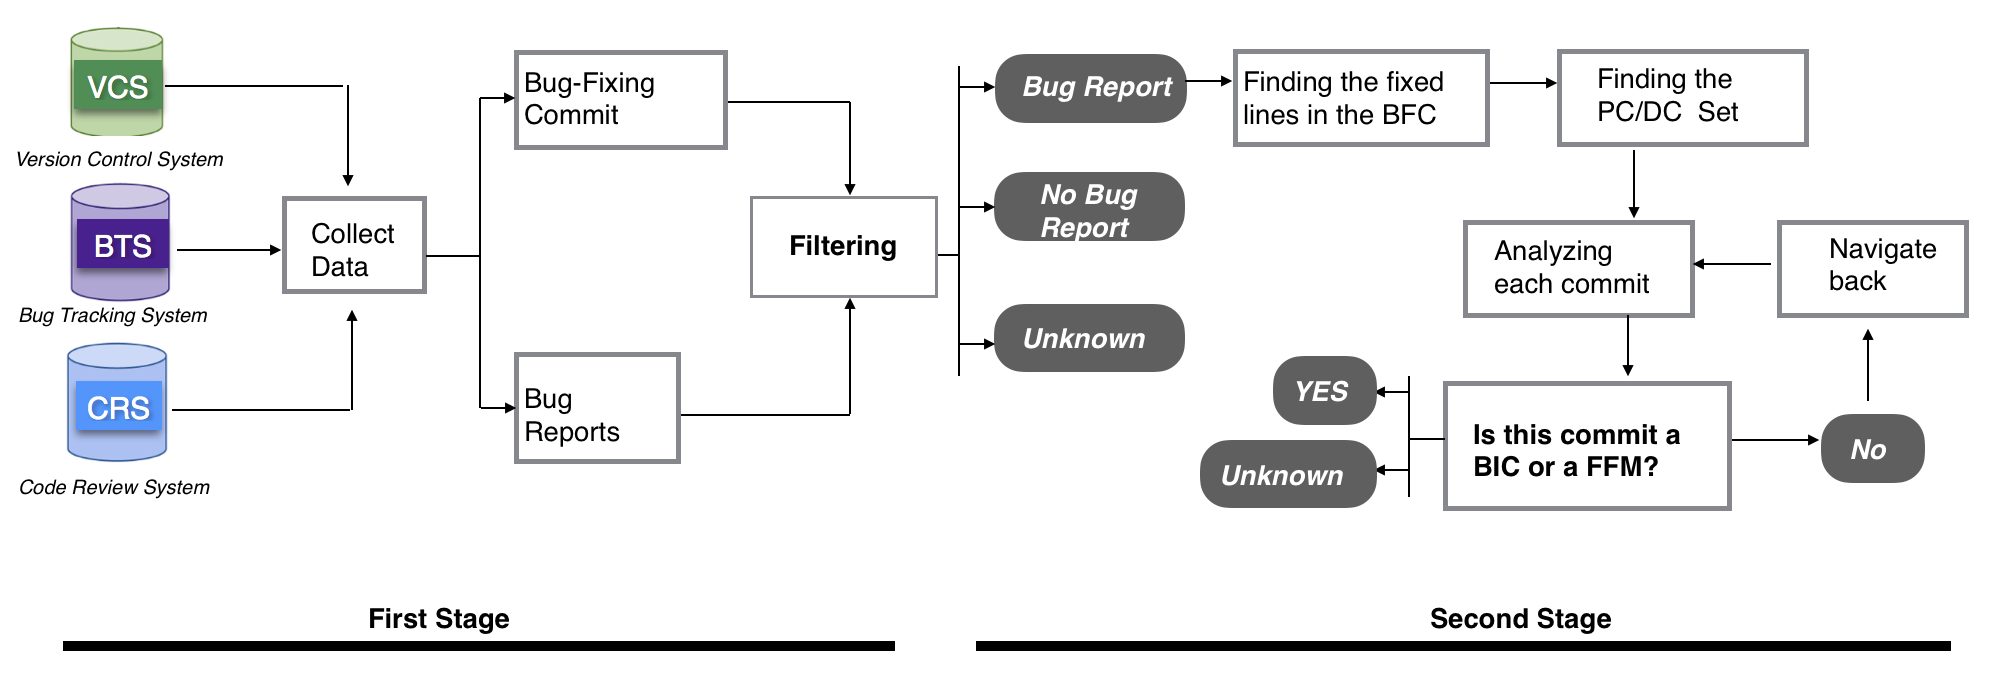
\includegraphics[width=\columnwidth]{img/diagram.png}
\caption{Overview of the steps involved in our analysis \gema{I need to modify the steps, writing the FFC instead of BIC} }
\label{fig:diagram}       % Give a unique label
\end{figure}


\subsection{First Stage: Filtering}
\label{sec:methodologyFS}

This stage ensures that the bug reports stored in the datasets can be applicable to out model. Despite the strict policy of bug labelling in ElasticSearch and the agreement on classifying bug reports from other issues in Nova, this stage analyzed carefully each piece of information in the bug reports to ensure the ``gold standard". Thus, the dataset should only store bugs that are considered bugs at the moment of bug fixing. For example, there is a (hypothetical) test that fails right before the bug-fixing commit, and does not fail right after it.  This also means that if there are issues that are reported as bugs but are rather new feature requests or improvement suggestions as discussed are excluded. 

\subsection{Second Stage: Identifying the First Failing Commit and the Bug Introducing Commit of a bug report}
\label{sec:methodologySS}

The input of this stage is a set of bug report from Nova and ElasticSearch that describe bugs in the moment of bug fixing. The steps in this stage consists on manually identify the corresponding Bug-Introducing commit and the First-Failing commit for a Bug-fixing commit, or decide that there is not a \BIC. The identification of \BIC given a \BFC means that the bug was present at the time commit the lines. Since the \BIC can be in the previous commit or in any of the descendent or antecesor commits, it is necessary to manually analyze them in order to ensure the credibility of the ``gold standard". In the cases where the bug was not present at the time of writing the lines, then there is not a \BIC, it is necessary to find the \FFC. To better understand this process, the steps are detailed in the following paragraphs. Remember the terminology described in section 5.1.1 that explains concepts such as \BFC, \setBFC{b}, \PC{b}, \ACSet{b} ..., etc. 

%Requirements have changed invalidating previous assumptions (GDPR). In this case there is no bug introducing commit.
%External resources have been modified (GitHub API). In this case there is no bug introducing commit.
%Internal resources have been modified (directory structure and permissions; the Chromium bug). In this case there is a bug introducing commit but this commit did not directly affect the lines of code modified in the bug fixing commit, so SZZ cannot find it; this bug introducing commit would have taken place after the previous commit and before bug reporting. 

\subsubsection{Finding the lines that fixed the bug}

At this stage, we have to find the source code that fixed the bug, notice that a generic bug is referred as $b$. Therefore, we have to:
	\begin{itemize}
		\item Identify the change(s) that fixed the bug,\setBFC{b}. In most of the analyzed cases this set was always singleton, it means that in each bug there is an unique \BFC. But, in the bug report \#1442795\footnote{\url{https://bugs.launchpad.net/nova/+bug/1442795}} there are two different \BFC that really fixed the bug. However to simplify, this methodology assumes that the \setBFC{b} is singleton, and in the case where more than one \BFC fixed the bug, the methodology will analyzed both bug-fixing commit.
		\item Find the lines that the \setBFC{b} touched to fix the bug, \LC{c} where $c$ is the \BFC:
	In the bug fixing commit linked to a bug report, there is all the information related with the code review process. By applying \textit{``git diff''} we can identify what lines have been added, modified or deleted between the version after the \setBFC{b} and the previous one. There also exist the possibility of visualize these changes between the version after the \setBFC{b} and the previous one
 commit using GitHub. GitHub provides a friendly visualization.
 		\item Filter out lines that are not code:
		Lines that have been modified, but do not contain source code (e.g., comments or blank lines) are not considered, and as a consequence they are not analyzed. In addition, there was a \BFC\footnote{\url{https://github.com/elastic/elasticsearch/commit/beaa9153a629c0950182e4e8c4f8eedd1c63f49f}} that closed two different bug reports. In this case, the lines related to the other bug was filtered out.	
	\end{itemize}

\subsubsection{Determining, for each of those lines, \LC{c}, what commit changed these lines for the last time}

Each individual line touched by the \BFC has only one previous commit. However, there could potentially be as many previous commits as modified lines in the \BFC, see the genealogy tree in subsection 5.1.2. Thus, taking this genealogy tree as reference, the result is a set of all previous commits of the bug $b$, \PC{b}.  

\subsubsection{Analyzing each of these previous commit, and their descendent commits, to determine the \BIC and the \FFC}

This analysis uses information available in the description of the ticket and from the logs of the \BFC and commits in the set of \PC{b}. After understanding the bug and the changes that fixed the bug. It is necessary to identify the \BIC, if it exists, and the \FFC.Thus, the identification of the \BIC starts with the the analysis of the \PC{b}, for each of the \PC{b} the lines changed are analyzed in order to find which one introduced the bug. At this point, there is three different scenarios and the behaviour is different depending where we are:
\begin{enumerate}
	\item \textit{The commit inserted the bug}: This commit is the \BIC because it inserted the buggy lines at the moment of their writing. We were able to identify the \BIC and it is also the \FFC because it is the first commit that manifested the wrong behaviour. According to the theoretical model, the TSB passes in the \BFC and the \BIS is one of the snapshot of a previous commit of the \BFC.
	\item \textit{The commit does not insert the bug}: In this case there will be two possible outcomes:
		\begin{itemize}
			\item The lines in the commit are correct, they do not insert the bug at the time of their writing and other factors caused that these lines became to be buggy. There is no \BIC in this scenario and the analysis should be focuses on understand whether this pc is the \FFC or not. According to the theoretical model, the TSB is run in all the \ACSet{b} and it passes in the \BFC but it fails always in the antecessor snapshots. However, if we change the environment,  the TSB fails in the \BFC but it passes in the snapshot, and the first \BIS that passes in the sequence of \BIS is the \FFC.
			\item The lines in the commit are syntactic sugar and semantically equivalent modifications (refactorings): This means that the commit remains with the same behaviour than before, thereby we need to navigate back into, the \DCSet{b} and start again in the first point of this list..
		\end{itemize}
	\item \textit{It is not sure that the commit inserted the bug}: In this case we need to continue navigating back into the \DCSet{b}, if this commit inserted by first time the descendent lines of the \LC{c} and we are not sure if they are buggy or not, we can classify this commit as ``undecided". This means that after the analysis we were unable to manually find the \BIC despite it exists, or that we were unable to find the \FFC or \BIC because we did not have enough context.
\end{enumerate}


\subsection{Outcomes}

At the end of the process there are three possible outcomes for each bug report analyzed. The outcomes are related with the unequivocally identification of the \BIC and \FFC given a \BFC.
These outcomes are explained in the following list:  %\subsubsection{Tickets}

%There are three possible outcomes for each bug report analyzed:
\begin{itemize}
	\item A bug report has a Bug-Introducing Change: In this case we are sure that there is at least one bug introducing change among the previous commit set, descendent commit set or ancestor commits set. However, during the manual analysis it may occur that:
		\begin{enumerate}
			\item We were able to manually identify this moment or,
			\item We were unable to manually identify this moment.
		\end{enumerate}
		Furthermore, in this scenario, the \BIC is also the \FFC.
	\item A bug report does not have a Bug-Introducing Change: In this case, we are sure that any line contained the bug when it was committed into the source code, and other factors such as modification in internal resources, changes in external resources, buggy code in third-parties or changes in the requirements invalidate previous assumptions are the cause of the bug-fixing commit. And, none of the antecesor commits has inserted the wrong lines, thereby we can not blame any of them and we are only able to identify the first time that the bug manifested in the code. Also, in this case it may occur that:
	\begin{enumerate}
			\item We were able to manually identify the \FFC or,
			\item We were unable to manually identify the \FFC.
		\end{enumerate}
	\item It is not clear whether or not a bug report has a Bug-Introducing Change: Some bugs report does not detail enough information about the failure and the bug fixing commit is not enough to decide whether or not there is a \BIC. Also, some commits are very complex to understand their changes and we can not decide whether it inserted the bug or not.

\end{itemize}

%\begin{itemize}
%	\item Does not exist a \FFC in the set of ancestral commits \ACSet{b} because the ticket was classified into (1) Undecidable \FFC or (2) $ \FFC \notin= \ACS$. Therefore, there is not any buggy line in the \ACS of the \BFC, and we ware only able to find the first commit in which the bug manifested. We will refer this set of tickets as \textit{``Without Bug''}.
%	\item A \FFC exists in the set of ancestral commits \ACSet{b}: In this case we found a the bug introducing change among the ancestral commits. We will refer this et of tickets as \textit{``Bug''}. Furthermore, the \FFC of each ticket could be in one on the following sets:
%		\begin{enumerate}
%			\item $\FFC \in \PC{b}$ : The bug introducing change are found in the \PC{b} set.
%			\item $\FFC \notin \PC{b}$ : The bug introducing change are not found in the \PC{b} set but it belongs to the \ACSet{b} set.
%		\end{enumerate}
%\end{itemize}
%
%\subsubsection{Commits}
%
%There are three possible outcomes for each commit analyzed:
%\begin{itemize}
%	\item It is the first failing change, the change caused the later fixed%. Also, we could classify each bug introducing change as:
%%	\begin{enumerate}
%%		\item \BIC's found with SZZ: When the algorithm is able to locate the $pc$, and it is a true positive.
%%		\item \BIC's not found with SZZ: When the \FC only added new lines since some $pc$ forgot to add, (i.e, an if/else condition). The SZZ algorithm could not found it because it discards these situations.
%%	\end{enumerate}
%	\item It is the closer first failing change.
%	\item It is not a (closer) first failing change, the change did not cause the bug. %In addition, according to SZZ algorithm this commit is false positive because the algorithm is able to locate it but it is not the cause of the failure.
%\end{itemize}
%
% we select the lines of each \pc belonging to the \PC{b} and navigate back into the \ACS of these lines until find the line, if it is applicable, that caused the bug. As a result, we could be in one of these situations in order to determine the \FFC:
%\begin{itemize}
%	\item $ Undecidable \FFC $, i.e.,  when we cannot be sure to find the \FFC between all ancestral changes.
%	\item $ \FFC \notin= \ACS$, the bug has been caused by external dependencies: (1) Bug in dependencies or (2) Bug in API's.
%	\item $ \FFC \in = \ACS$, the bug has been caused by a change belonging to the chain of ancestor changes of the bug \ACSet{b}.
%\end{itemize}
%

\section{Results}
\label{sec:results}
This section presents the results of the empirical analysis in order to locate the \BIC and the \FFC in two cases study, Nova and ElasticSearch. Furthermore, there is a comparison between the results obtained after applying the proposed model with the results obtained with the tradicional SZZ algorithm found in the current literature.

\subsection{First Stage}
\label{sec:resultsFS}

%This stage is only applicable to OpenStack. We randomly selected 125 tickets from the Nova and classified them using the Bugtracking tool~\cite{rodriguez2016bugtracking}. In 87 of the cases, the independent researchers agreed in the classification of the ticket, that is, their results matched in 70\% of the cases. Of those, 67 tickets had been classified as bugs, 16 as not bugs, and 4 as \emph{undecided}.

From the 120 bug report classified as bug reports in both projects, 58 from Nova and 58 from ES were considered in the next stage. The main reason was the discordance between the developers to classify them as bug. For example, there are some comments in the bug \#1185290 \footnote{\url{https://bugs.launchpad.net/nova/+bug/1185290}} where this discordance is obvious:
	\begin{itemize}
		\item `` I am not sure that I consider this a bug. Without --all-tenants=1, the code operates under your own tenant. That means that --all-tenants=1 foo should really be a no-op without --all-tenants=1. "
		\item `` I disagree, mainly because the structure of the requests and code path should largely be transparent to the user. I would suggest that specifying --tenants should imply you are doing a query across --all-tenants=1unless the --tenants specified is the same as what is contained in OS\_TENANT\_NAME (the unless part is debatable)"
	\end{itemize}

Nevertheless, other reasons also were found, for instance the bug \#1431571 \footnote{\url{https://bugs.launchpad.net/nova/+bug/1431571}} reported a bug in a test file. We removed it from the analysis because a bug in a test file does not mean that the source code of the project may contain a bug. And, we also found that some bug reports such as \#1814\footnote{\url{https://github.com/elastic/elasticsearch/issues/1814}}, \#7740\footnote{\url{https://github.com/elastic/elasticsearch/issues/7740}} and \#1448075\footnote{\url{https://bugs.launchpad.net/nova/+bug/1448075}} are describing hypothetical scenarios. In these cases the bug description details a possible bug in the future, and we need to remove them from the analysis because despite the developers describe them as bug report, we understand that at the moment of submitting the bug-fixing change, the bug is not present in the project. 

\subsection{Second Stage}
\label{sec:resultsSS}

The main goal of this chapter is to apply the proposed model described in Chapter 5 to identify what are bug-introducing commits, and how they are related to bug-fixing commits. This model allows to define the ``gold standard" of which \BIC in Nova and ElasticSearch correspond with the \BFC. This chapter answers two different questions:

The first part presents the results after applying the model to the data set. Thus, to demonstrate how the model works, we gathered a set of \BFC from two projects, and find out (manually) their \BIC when it exists. As it is mentioned before, we apply the definitions of \BIC and \BFC based on the existence of a \TSB. In case we cannot find the \BIC, we could consider excluding the corresponding \BFC from the study, since the empirical study is focused in the cases when \BIC can be found or when we are sure it does not exist. 

The second part presents the effectiveness of SZZ-like algorithm. Once we have the ``gold standard" we can evaluate how SZZ-like algorithms ``really" perform which it is an important contribution to the current literature because as far as we know, any researcher have carried out this empirical anlaysis. 

%Furthermore, to ensure we have understand the description of the bug, we contacted with two developers of ElasticSearch that participated during the bug-fixing process of the tickets analyzed. And, we asked them to classify the 60 tickets between \BIC, \NoBIC or \emph{Undecided} depending on the ticket analyzed was describing that the behavior was buggy from the beginning (\BIC), the behavior became buggy as the system had evolved or the bug was caused by other aspects (\NoBIC), and in case of doubts they classified the ticket as \emph{Undecided}. The agreement between the two experts and the first author was measured with the \emph{Fleiss' kappa} which is a statistical measure for assessing the reliability of agreement between a number of rates when assigning a classification of a number of items in different groups~\cite{warrens2010inequalities}. The overall agreement measured was 0.527778 which means a moderate agreement which indicates that despite of the first author is not an expert in the project she has enough experience to carry out this analysis and the results are significant, at least as start point to understand the origin of the bugs and all the elements that take place in this complex phenomenon.

%On the other hand, we also have contacted with developers from OpenStack that participated during the bug-fixing process of the tickets selected but, due to the fact they are continuously changing from project and companies none of them could answer in a proper way that question. From this point in advance, we will take the analysis of the first author to find the \FFC. Notice, that when the first author have doubt about the classification of some ticket, she asked some of the other author in order to give an external view and confirm/discuss her opinion.


\subsection{ RQ1:What is the frequency for a bug-fixing commit being induced by a bug-introducing commit?}
Table~\ref{tableBugNoBug} shows the number of bug-fixing commit that have been induced by a bug-introducing commit and the number of bug-fixing commit that have not been induced by a bug-introducing commit. It is noticed that in ElasticSearch the number of bug-fixing commit induced by a \BIC is higher than in Nova, and probably the reason is the programming language. While Python is a dynamic language that can be run without compile it before, Java is strictly typed and performing run-time checks. 
\begin{table}[!t]
	\renewcommand{\arraystretch}{1.3}
	\caption{Percentage of Bug-Fixing Commit with a Bug-Introducing commit \emph{BIC}, without a Bug-Introducing Commit \emph{NO\_BIC} and Undecided..}
	\label{tableBugNoBug}
	\centering
	\begin{tabular}{|c|c|c|c| }
		\hline
  		&  BIC & NO\_BIC & Undecided \\
		\hline
		\hline
		Nova & 38 (65\%) & 14 (24\%) & 6 (10\%)\\
		\hline
		ES & 45 (77\%) &  6 (10\%) & 7 (12\%)\\
		\hline
	\end{tabular}
\end{table}

\subsubsection{RQ1.1: Could the location of a bug be modeled on the bug-introducing moment and first failing moment?}

Table~\ref{tableBICFFC} shows the percentage of \BIC and \FFC that have been manually identified by using the model. By definition, in theory our model is able to identify the \FFC and the \BIC whether it exists, but in practise, since the identification needs to be done manually, sometimes we did not identify the \BIC or the \FFC. Thus, for the 58 \FFC and 38 \BIC belongs to Nova dataset, we successfully identify 40 \FFC and 25 \BIC.
In the dataset of ElasticSearch, from the 60 \FFC and 45 \BIC, we successfully identify 49 \FFC and 34 \BIC.

\begin{table}[!t]
	\renewcommand{\arraystretch}{1.3}
	\caption{Percentage of Bug-Introduced Commit and First Failing Commits identified after applying the theoretical model.}
	\label{tableBICFFC}
	\centering
	\begin{tabular}{|c|c|c|c|}
		\hline
  		&  BIC & FFC & Undecided \\
		\hline
		\hline
		Nova & 25 (66\%) & 40 (69\%) & 18 (31\%)\\
		\hline
		ES & 36 (80\%) &  48 (83\%) & 10 (17\%)\\
		\hline
	\end{tabular}
\end{table}

\subsubsection{RQ1.2: Which reasons may cause that a bug-fixing commit is not induced by a bug-introducing change?}
Additionally, in those cases where the bug report does not present a \BIC, we have looked for its cause. Table~\ref{tablereasosNoBIC} shows the main reasons for a bug not having a \BIC. 
\begin{table}[!t]
	\renewcommand{\arraystretch}{1.3}
	\caption{ Reasons why a bug-fixing commit is not induced by a bug-introduced commit }
	\label{tablereasosNoBIC}
	\centering
	\begin{tabular}{|c|c|c|}
		\hline
  		& Nova & ElasticSearch  \\
		\hline
		\hline
		Co-evolution Internal & 9 (50\%) & 2 (40\%) \\
		\hline
		Co-evolution External  & 3 (17\%) & 2 (27\%)\\
		\hline
		Compatibility & 2 (11\%) & 0 (0\%)\\
		\hline
		Bug in External API & 4 (22\%) & 2 (20\%)\\
		\hline
	\end{tabular}
\end{table}
Furthermore, they are explained below:
\begin{itemize}
 	\item \textit{Co-evolution Internal}: Changes in the source code related to satisfy the new requirements of the project. Since internal resources have been modified (directory structure and permissions) or requirements have changed invalidating previous assumptions.  	
	\item \textit{Co-evolution External}: Bugs are caused by some external change. External resources have been modified without a previous notification and the source code of the project starts to fail.
  	\item \textit{Incompatibility}: Bugs are caused by an incompatibility between software and hardware or an incompatibility with some operating systems.
  	\item \textit{Bug in External API}: A change in the API of a third-party code caused a bug in the source code of the project.
\end{itemize}

\gema{maybe make an inclusion list of all the scenarios}

%Table~\ref{tableFFC} shows the classification of the \FFC in Nova and ElasticSearch, depending on the kind of \FFC. \gema{Explicar a que se refiere cada una de las dos categorias}
%\begin{table}[!t]
%	\renewcommand{\arraystretch}{1.3}
%	\caption{Results of the analysis of the previous commits using both methods for Nova.}
%	\label{tableFFC}
%	\centering
%	\begin{tabular}{|c||c||c||c| }
%		\hline
%  		&  \FFC not in \ACS & \FFC in \ACS & \FFC in \emph{PC} \\
%		\hline
%		ES & (\%) &  (\%) &  (\%)\\
%		Nova & (\%) &  (\%) & (\%)\\
%		\hline
%	\end{tabular}
%\end{table}

\vspace{0.2cm}
\fbox{\begin{minipage}{30em}
\textbf{RQ1: A bug-fixing commit is not always induced by a bug-introducing commit and depending on the programming language used in the project this situation is more frequent. The main reasons why a bug-introducing commit is not present in a bug-fixing commit is the co-evolution internal and external.}
\end{minipage}}
\vspace{0.1cm}

\subsection{ RQ2: What are the specifications that define the effectiveness of an algorithm used to locate the origin of a bug? }
After applying the model and identifying the number of \BIC and \FFC in our dataset, we have the ``gold standard" in which we can be sure of the number of bug-fixing commit with a bug-introducing change and without a bug-introducing change. For that reason, we are able to really compute the true/false positives/negatives for an algorithm, and for that purpose we have chosen the SZZ-1 algorithm~\cite{kim2008classifying}, which is an enhancement proposed by Kim~\textit{et al.} of the SZZ. 

The SZZ-1 algorithm does not compute the bug-fixing changes with only new lines added, and in the ``gold standard" of Nova there are tree \BFC with only new lines whereas in ElasticSearch there are seven. These cases are the false negatives of the SZZ-1. Furthermore, in some \BFC, the SZZ-1 algorithm identifies more than on possible bug-introduction change, in this case if the \BFC was induced by a \BIC and the SZZ-1 is able to identify it, we compute one true positive and the rest of possible bug-introduction change as false negatives. On the contrary, if the SZZ-1 is not able to identify the \BIC between the set of possible bug-introduction changes, we compute all of them as false positives.  

The ``gold standard" of Nova consists of 25 Bug-Fixing commit with a bug-introducing change and six bug-fixing commits without a bug-introducing change. While the ``gold standard" of ElasticSearch is made up 36 bug-fixing commit with a bug-introducing change and six bug-fixing commits without a bug-introducing change. When applying the SZZ-1 algorithm to the set 31 \BFC of Nova, it returns a set of 63 possible bug-introduction changes. And when the algorithm is applied to the 42 \BFC of ElasticSearch, it returns a set of 73 possible bug-introduction changes. Table~\ref{realSZZ} presents the percentage of true/false positives/negatives for the SZZ-1 as well as the precision and recall.
%We compare SZZ with the ?gold standard?, and also SZZ-token (SZZ, but considering tokens, as dmg does it, instead of lines), and/or other SZZ variants. The main contribution of this part is to show how really to compute true/false positives/negatives for an algorithm, since we can compare with our gold standard in our two petty cases. 

\begin{table}[!t]
	\renewcommand{\arraystretch}{1.3}
	\caption{Results of True Positives, True Negatives, False Negatives, Recall and Precision for the SZZ-1 algorithm assuming that the algorithm flags all of the commits belong to a set of \PC{b} as \BIC.}
	\label{realSZZ}
	\centering
	\begin{tabular}{|c|c|c|c|c|c|}
		\hline
 	 	&  True Positives & False Positives & False Negatives & Recall & Precision \\
		\hline
		\hline
		Nova & 22 (33\%) & 41 (62\%) & 3 (5\%) & 0.88 & 0.35\\
		\hline
		ES &  26 (33\%) & 47 (60\%) & 7 (9\%)& 0.79 & 0.36 \\
		\hline
	\end{tabular}
\end{table}

In the literature there is no clear the heuristic followed by some researchers when the SZZ identifies a set of possible bug-introduction changes for a Bug-fixing commit. In Table~\ref{realSZZ} we assume that whether this case occurs, the researchers flag all of the commits belong to that set as a possible bug-introduction changes. However, some researchers in the literature state that whether this case exists the bug-introduction change is the earlier one in time. With this assumption, we have compute again the number of true/false positives/negatives of the SZZ-1 using the ``gold standard" of Nova and ElasticSearch. Now, when applying the SZZ-1 to the 31 \BFC of Nova, it returns a set of 28 possible bug-introduction changes. And, when SZZ-1 is applied to the 42 \BFC of ElasticSearch, it returns a set of 35 possible bug-introduction changes. Table~\ref{realSZZ2} presents the percentage of true/false positives/negatives for the SZZ-1 as well as the precision and recall in this scenario.
%We compare SZZ with the ?gold standard?, and also SZZ-token (SZZ, but considering tokens, as dmg does it, instead of lines), and/or other SZZ variants. The main contribution of this part is to show how really to compute true/false positives/negatives for an algorithm, since we can compare with our gold standard in our two petty cases. 

\begin{table}[!t]
	\renewcommand{\arraystretch}{1.3}
	\caption{Results of True Positives, True Negatives, False Negatives, Recall and Precision for the SZZ-1 algorithm assuming that the algorithm only flags the earlier commits that belongs to a set of \PC{b} as \BIC.}
	\label{realSZZ2}
	\centering
	\begin{tabular}{|c|c|c|c|c|c|}
		\hline
 	 	&  True Positives & False Positives & False Negatives & Recall & Precision \\
		\hline
		\hline
		Nova & 21 (68\%) & 8 (26\%) & 2 (6\%) & 0.91 & 0.72\\
		\hline
		ES &  19 (45\%) & 16 (38\%) & 7 (17\%)& 0.73 & 0.54 \\
		\hline
	\end{tabular}
\end{table}


\gema{el estudio de tokens para los falsos positivos que encontramos en nova y en ES??}

\vspace{0.2cm}
\fbox{\begin{minipage}{30em}
\textbf{RQ2: In the best scenario applying the heuristics of the SZZ-1, Nova computes 26\% of false positives with a precision of 0.72 and a recall of 0.91. ElasticSearch presents higher percentage of false positives (38\%) than Nova, and lower precision (0.73) and recall (0.54).}
\end{minipage}}
\vspace{0.1cm}

\gema{RQ sobre como afecta TTN y el BFT y developer en la grand verdad ? }

%%%%%%%%%%%%%%%%%%%%%%%%%%%%%%%%%%%%%%%%%%%%%%%%%%%%%%%%%%%%%%%%%%%%%%%%%%%%%%%%
%%%%%%%%%%%%%%%%%%%%%%%%%%%%%%%%%%%%%%%%%%%%%%%%%%%%%%%%%%%%%%%%%%%%%%%%%%%%%%%%
% DiSSCUSSION %
%%%%%%%%%%%%%%%%%%%%%%%%%%%%%%%%%%%%%%%%%%%%%%%%%%%%%%%%%%%%%%%%%%%%%%%%%%%%%%%%

\cleardoublepage
\chapter{Disscussion}
\label{chap:discussion}
In this concluding chapter, we recapitulate the contributions of our study over time, we discuss the findings and describe lessons learned and threats to validity. Finally, we draw some lines of our future research.

\section{Threats to validity}
\label{sec:threats}

The limited sample size of tickets used in this research is the major threat to its validity. It may happen, that only with 120 seemingly random bug reports, there may be a prior unknown tendency. This is in fact similar to~\cite{sliwerski2005changes}, where the trend indicates that most bugs are fixed on Fridays.
The main threat to validity is the number of tickets considered. It is relatively high, but there is a long way to get a representative sample from a variety of free/open source systems, or software projects at large. Our analysis requires a lot of human effort, so increasing meaningfully the number of tickets is difficult. However, it should be noted that our numbers are the order of magnitude of similar studies: for instance Hindle's \emph{et al.} ~\cite{hindle2008large} article on large commits, considered 100 commits.

\subsection{Construct validity}
\subsection{Internal validity}
Other internal threats to validity are:

\begin{itemize}
    \item
    \item 
    \item
    %\item Although the researchers are experienced programmers, they are not experts in the  OpenStack and ElasticSearch projects, and their inexperience may have influenced the results of the analysis.
    \item 
    %\item We have used a random script to extract the tickets from Launchpad that have been reported during 2015. There could be unintended bias of the data, because many reasons, as for instance the phase of the project.
    \item
\end{itemize}

\subsection{External validity}
The most important external threats, most of them related to peculiarities of the Nova project, are:

\begin{itemize}
    \item 
    \item 
    \item 
\end{itemize}


\section{Discussion Chapters}
\subsection{Reproducibility and Credibility of the SZZ Discussion}
\label{subsec:implicationsSZZ}

We consider it important to highlight some of the lessons learned after performing this SLR. It turns out that, when empirical studies are based on heuristics or assumptions, authors must be conscious that to produce reproducible studies the best method is to include a replication package that can be publicly available together with its publication (ideally, for ever). Researchers have however to be aware that some issues, such as the software environments, might change, causing that both programs and data become obsolete, so a detailed description of the elements, methods and software used during the study is also valuable.

On the other hand, to provide more trustable results, we recommend that researchers specify (and argue) the use of those methods/algorithms that mitigate the limitations of their studies, be aware of the risk of every assumptions that is being used and, if needed, provide a manual analysis of the results. For those studies where the study size is large, researchers can select a random sample to validate it manually.

As it is the case in software projects with release numbering~\cite{israeli2010linux}, it would be desirable to have a similar mechanism for software implementations used in such type of research, although this may not always be possible given the decentralized nature of research. We, therefore, recommend researchers who develop modifications to the SZZ algorithm to publish the software implementation in development sites such as \texttt{GitHub}, so other researchers can \emph{fork} the project. These \emph{forks} could be easily traced, and the authors could ask for a specific citation to their solution if other researchers make use of it.

Finally, we offer a simple way to measure the ease of reproducibility and credibility of research papers. Even if this measure has been conceived with those studies that make use of SZZ in mind, we think it can be adapted to other ESE research easily. Thus, authors can easily assess if their paper offers a reproducible and trustable work (i.e., with scores above or equal to 5). Although we have often addressed authors directly, we should not forget the responsibility of reviewers in the scientific process. We have seen that authors are often detail-focused when presenting their research --in favor our intuition, we have found that reproducibility is related with being aware of the limitations --, but reviewers should have the required vision to evaluate the studies taking these details into consideration, and helping authors to raise the level of their research. Thus, we recommend reviewers to ask themselves the questions, adapted to the context of the research, proposed in Section when performing a review of a paper using heuristics and assumptions.

In this paper we have studied the use of SZZ, a widely used algorithm in ESE research. We have shown that SZZ is certainly relevant, and that it is not limited to a niche audience, but has spread to be an important component of publications in top journals and prominent conferences. In this regard, we can see its study as a case study of how a software engineering practice spreads across academia.

We have observed that limitations to SZZ are well known and documented. Improvements have been proposed, with unequal success up to the moment. While the limitations to its first part --related to linking fix commits and bug tracking issues-- has improved significantly, the enhancements for the second part --that has to do with finding the bug introducing change-- are still limited and accuracy has room for improvement.

Even if limitations have been widely documented, from our study we can see that this has not made ESE practices stronger. From the detailed study of the threats to validity of publications using SZZ, SZZ-1 and SZZ-2, we have seen that most publications are not reporting the limitations, and interestingly enough, limitations to the first part --which have shown to be less relevant-- are discussed more often than those to the second part. The fact that 37\% of the publications use the \emph{original} SZZ is indicative in this regard.

We have found that reproducibility of the publications is limited, and replication packages are offered seldom. The results presented in our research are in line with previous research~\cite{amann2015software}, although not as \emph{bad} as the ones found for MSR in 2010~\cite{robles2010replicating}. In any case, we think they are not satisfactory enough, and should raise some reflexions about the scientific methods used in our discipline.

Even if using one of the improved versions of the algorithm helps in the accuracy of the SZZ approach as pointed out in~\cite{rahman2012clones}: ``Accuracy in identifying bug introducing changes may be increased by using advanced algorithms (Kim et al. 2006, 2008)'', they are seldom used -- only 22\% of the publications use one of the two (improved) revisions of SZZ. It seems that researchers prefer to \emph{reinvent the wheel}, 49\% use an ad-hoc \emph{modified} version of SZZ in their publications, than to use others' improvements. One possible reason for this is that papers that describe the SZZ algorithm or any of its improvements do not provide a software implementation. Thus, researchers have to implement it from scratch for their investigation. Our results show that in such a situation what is done is taking the base SZZ algorithm and then adding some modifications, resulting in an 'ad-hoc' solution. For all 'ad-hoc' solutions identified, we have not found a rationale of why other enhancements to SZZ have not been implemented. Another major problem when using improvements to SZZ is that they have not been given a version/label. Even if a revision of SZZ is used, publications often refer to it as SZZ, making it difficult to follow, to reproduce, to replicate and to raise awareness on this issue.

We have observed that full comprehensive reports of reproducibility are seldom found, we classified only 15\% of the papers as being \emph{good and excellent quality with respect to reproducibility}. The research community should direct more attention to these aspects; we believe that too much attention is put on the final result(s) (the \emph{product} of the research: new knowledge) in comparison to the research process. As researchers in the field of software engineering, we know that both --a high quality product and process- are essential for a successful advancement in the long term~\cite{kan2002metrics}.

All these factors undermine the credibility of ESE research, and require a profound consideration  by the research community
\gema{Como afecta las asunciones hechas en la credibilidad de los resultados}

\subsection{Theoretical Model Discussion}
\label{subsec:implicationsModel}
After analyzing several bugs in this study, we have realized as well that determining where and when a bug was introduced is not a trivial task. In fact, even just determining if the bug was present at the time a certain commit introduced the code that latter triggered it is in some cases not easy at all.

For example, we have found some cases where we the current automatic techniques are unable to determine the point of introduction of the bug, as no previous commit can be identified. One of those cases is when the fix only adds code: in such case there is no way of identifying the previous commit as we defined it, since there is no previous commit touching the fixing lines. In this case, only the description of the ticket or the \BFC could clarify either the new lines were not included due to an error causing that some  ancestor commit is the cause of the bug or they were included in the \BFC because of the later introduction of some new functionality, and thus the line in the ancestor commits was correct at the time it was introduced causing that the \BFC does not have a BIC. Thus, studies based on SZZ removed the \BFC that only adds new lines to fix the bug because they can not track back such lines, and as a consequence this lead to mislead the results, showing higher percentage of accuracy.

Furthermore, many researchers have based their methods to locate the bug-introducing change in the SZZ algorithm or they may have used datasets to feed their bug prediction or classification models with results obtained form the SZZ such as Ray~\emph{et al.} that used a dataset from \~cite{rahman2014comparing} which was gathered using the SZZ algorithm to study the naturalness of buggy code~\cite{ray2016naturalness}. Massacci~\emph{et al.} evaluated most existing vulnerabilities discovery models on web browsers and took many datasets where at least the built in~\cite{neuhaus2007predicting} used the SZZ approach ~\cite{massacci2014empirical}. And, Abreu~\emph{et al.} uses the data set obtained in ~\cite{sliwerski2005changes} to study how the frequency of communication between developers affects the fact to introduce a bug in the source code~\cite{abreu2009developer}.


All in all, we believe in the benefit that this new concept to locate the \FFC has in the Software engineering. In addition, with the classification of the origin of the bugs, we seed some more lights in the problem of emulating software faults realistically. However, to achieve greater bug location automation, we therefore need a concerted effort in testing to find ways or techniques to address the re-built problem and to build a test that can be automated or partially automated to find the \FFC.% Also, it will be necessary to define how to use this information in a technique to inject these kind of bugs because they are not as obvious as the classical fault injection that emulates hardware faults.


\subsection{Results Discussion}



%%%%%%%%%%%%%%%%%%%%%%%%%%%%%%%%%%%%%%%%%%%%%%%%%%%%%%%%%%%%%%%%%%%%%%%%%%%%%%%%
%%%%%%%%%%%%%%%%%%%%%%%%%%%%%%%%%%%%%%%%%%%%%%%%%%%%%%%%%%%%%%%%%%%%%%%%%%%%%%%%
% CONCLUSIONS AND FUTURE RESEARCH %
%%%%%%%%%%%%%%%%%%%%%%%%%%%%%%%%%%%%%%%%%%%%%%%%%%%%%%%%%%%%%%%%%%%%%%%%%%%%%%%%

\cleardoublepage
\chapter{Conclusions and Future Research}
\label{chap:conclusions}
In this concluding chapter, we recapitulate the contributions of our study over time, we discuss the findings and describe lessons learned and threats to validity. Finally, we draw some lines of our future research.


This article has presented a detailed definition of the FFC that includes its dependencies and the different classes to be grouped. In addition, the empirical experiment we have performed in Nova and ElasticSearch has shown that for a large fraction of the analyzed tickets, Gema says: Write percentage, presented a FFC due to external artifacts. Whereas from those tickets where a FFC can be clearly found in the chain of precedence, the implicit assumption that bugs were introduced in the previous commit does not hold at least in Gema says: Write percentage of them.
Also, we have traced a guide with the rules to define the effectiveness of an approach in order to find the FFC and we have described some of the reasons why looking for the BIC or using some heuristics to predict bugs are not the best option whether our purpose is reduce the error in the results or predictions.

\section{Conclusions}



\section{Future Work}
\label{sec:future}
Once we have found that at least manually we can identify the FFC us- ing the criterion established and theoretically we were able to classify them depending their nature. It makes sense to automatize the test idea to find the FFC, as future work, to which extent this happens in an optimal project where we could have all the dependencies under control and probably use higher number of tickets.
Of course, another future line is a detailed classification, in different projects, of all the cases of introduction of bugs that are not related to the previous changes but can be automatically detectable. This could help to better design- ing integration tests, to better check for those cases.
The full automation of the methodology used in this paper is also interesting from a practical point of view. That would provide software projects with a valuable tool for understanding how they are introducing bugs, and therefore design measures for mitigation.


%%%%%%%%%%%%%%%%%%%%%%%%%%%%%%%%%%%%%%%%%%%%%%%%%%%%%%%%%%%%%%%%%%%%%%%%%%%%%%%%
%%%%%%%%%%%%%%%%%%%%%%%%%%%%%%%%%%%%%%%%%%%%%%%%%%%%%%%%%%%%%%%%%%%%%%%%%%%%%%%%
% APPENDIX %
%%%%%%%%%%%%%%%%%%%%%%%%%%%%%%%%%%%%%%%%%%%%%%%%%%%%%%%%%%%%%%%%%%%%%%%%%%%%%%%%

\cleardoublepage
\appendix
\chapter{Replicability of the Results}
\label{app:replicability}

Mining software repositories is a complex task in time, tools and datasets. Different authors have dealt with the issue of replicability in software engineering [Shull et al., 2008], [Basili et al., 1999]. In addition, Robles [Robles, 2010] and later in [Gonzlez-Barahona \& Robles, 2011] have raised a set of questions directly related to this problematic.
In first place, there are several elements that may be of interest for reproducibility:

\section{SLR}
\label{sec:replicabilitySLR}
\paragraph{Original data source}: the original data sources used along this dissertation can be found in \gema{url github}
\paragraph{Extraction methodology}: this methodology is briefly detailed in chapter 4, section ...., the paper introduce more details. While the scripts created and needed can be found at  \gema{url github}
\paragraph{Study parameters}: the initial filter applied over the raw data set is detailed in \gema{section chapter}.
\paragraph{Results dataset}:
\paragraph{Persistence}: it is expected to have access to the website as long as Github exists. 

\section{Empirical Study}
\label{sec:replicabilityEmpirical}
\paragraph{Original data source}:  the original data sources used along this dissertation can be found in \gema{url github}
\paragraph{Extraction methodology}: this methodology is detailed in chapter 6, section 6..... . While the scripts created and needed can be found at \gema{url github}
\paragraph{Study parameters}: the initial filter applied over the dataset is detailed in chapter 6 \gema{section chapter}.
\paragraph{Results dataset}:
\paragraph{Persistence}:  it is expected to have access to the website as long as Github exists. 


%%%%%%%%%%%%%%%%%%%%%%%%%%%%%%%%%%%%%%%%%%%%%%%%%%%%%%%%%%%%%%%%%%%%%%%%%%%%%%%%
%%%%%%%%%%%%%%%%%%%%%%%%%%%%%%%%%%%%%%%%%%%%%%%%%%%%%%%%%%%%%%%%%%%%%%%%%%%%%%%%
% APPENDIX %
%%%%%%%%%%%%%%%%%%%%%%%%%%%%%%%%%%%%%%%%%%%%%%%%%%%%%%%%%%%%%%%%%%%%%%%%%%%%%%%%

\cleardoublepage
%\appendix
\chapter{Resumen en Castellano}
\label{app:resumen}
\section{Introducci\'on}

Cuando un error ha sido reportado y posteriormente arreglado, no es tarea f\'acil identificar que cambio anterior realizado en el c\'odigo fuente indujo el posterior arreglo. Actualmente, los desarrolladores tienen a su disposici\'on multitud de informaci\'on almacenada en sistemas webs y sistemas de control de versiones sobre un determinado error y las acciones realizadas en el c\'odigo fuente para su arreglo.

Por un lado, existen applicaciones web basadas en el seguimiento de errores como por ejemplo, Bugzilla, Launchpad o Jira. Estas herramientas almacenan informaci\'on individual de cada uno de los errores encontrados en un sistema, esta informaci\'on ayuda a los desarolladores a entender mejor los errores y se presenta en forma de \emph{tickets}\footnote{Un ticket se refiere a una etiqueta/entrada describiendo cual es el error}, donde cada uno de ellos presenta una descripci\'on detallada del error, una lista enumerando las partes del projecto que se encuentran afectadas, las acciones necesarias para reproducir el error y, en ocasiones, comentarios de diferentes desarrolladores que aportan m\'as informaci\'on relativa al error. Por otro lado, exiten sitemas de control de versiones como Git, SVN o Mercurial, que tienen como prop\'osito llevar un registro de los cambios realizados en los archivos de un programa, y que brindan al usuario informaci\'on espec\'ifica sobre que lineas han sido eliminadas, a\~nadidas o modificadas en cada uno de los cambios realizados en el c\'odigo fuente del programa. Finalmente, las informaci\'ones de ambos sistemas puede ser vinculadas, lo que permite a un investigador entender cual ha sido el error y que acciones se han llevado a cabo en el c\'odigo fuente para arreglar el error.

Hasta el momento, las t\'ecnicas m\'as habituales usadas por los investigadores para identificar las lineas, que causaron el error se basan en la asunci\'on que ``dado una modificaci\'on en el c\'odigo que arregla un error, las l\'ineas que han sido modificadas o eliminadas son las potencialmente causantes de dicho error". Por lo tanto, si usamos el sistema de control de versiones para retroceder en la vida de dichas l\'ineas, el \'ultimo momento donde fueron modificadas o a\~nadidas, previo al arreglo, se considera como el momento en el que se introdujo el error. Sin embargo, los investigadores no pueden estar seguros sobre la veracidad de los resultados obtenidos tras aplicar estas t\'ecnicas, puesto que no existe un marco comparativo que indique lo que es correcto y lo que no y pueda ser usado por los investigadores. Adem\'as, tampoco existe una definici\'on clara y concisa de lo que significa introducir un \emph{error}, o de como definir el \emph{momento} en el que el error se introdujo. Esta falta de definiciones en la literatura actual, ha provocado que los investigadores tengan que asumir que el \'ultimo cambio realizado en las lineas posteriormente arregladas, fue el cambio que introdujo el error.

Teniendo todo esto en cuenta, esta tesis se enfoca en el estudio de la introducci\'on involuntaria de errores en el c\'odigo fuente. Concretamente, tiene el objetivo de modelar c\'omo se introducen los errores no intencionados en el c\'odigo fuente, creando un marco comparativo \'util para  comparar la \gema{performance en espanol} de otros algoritmos ya que \'este marco presenta la \gema{ground thruth en espanol}, siendo capaz de distinguir y localizar los dos momentos m\'as importantes para entender como se introdujeron los errores, estos momentos son:
\begin{itemize}
  \item momento de manifiestaci\'on del error:
  \item momento de insercci\'on del error:
\end{itemize}

Adem\'as, por definici\'on, el modelo propuesto en esta tesis contempla escenarios que son obviados en el an\'alisis actual, como por ejemplo cuando \'unicamente se introducen nuevas linas en el c\'odigo fuente para arreglar el error, estas lineas no puedes ser identificadas en la histora previa puestyo que no existian anteriormente, y por tanto, las t\'ecnicas actuales eliminan estos casos.

La falta de una definici\'on precisa sobre como identificar el momento en el que el sistema manifiesta el error por primera vez y el momento de insercci\'on del error ha dificulatdo el desarrollo de una t\'ecnica satisfactoria que identifique cuando un error se introdujo y cuando se manifesto. Debemos tener en cuenta que cuando nos referimos al `` momento en el que es sistema minifiesta el fallo por primera vez", no nos estamos refiriendo al momento en el que se report\'o el error o al momento en el que se introdujo el error. Imaginemos por un momento que para arreglar un error se ha modificado la linea n\'umero tres introducida en el momento \emph{A}, si usamos las t\'ecnicas actuales, la causa del error es la linea 3 insertada en el momento A. Sin embargo, si analizamos el contexto de esa linea y sus dependencias, podemos entender que a pesar de ser modificada para arreglar el error, esa l\'inea no introdujo el error en el momento A, si no que hubo un momento posterior, que denominaremos momento \emph{B}, en el que alg\'un cambios externo a nuestro programa, como modificaciones en la API, cambios en nuestro entorno o cambios en terceras partes del c\'odigo han afectado de alguna manera el comportamiento de  esa l\'inea provocando que en el momento B se manifestase el error en esa linea.

Por otro lado, tambi\'en existen factores que contribuyen a ocultar la verdadera causa del error, como por ejemplo: (i) \'unicamente se a\~naden nuevas lineas para arreglar el error~\cite{da2016framework}; (ii) repetidas modificaciones en las lineas que han sido modificadas para arreglar el error a lo largo de la historia del projecto dificultan el estudio de la evoluci\'on de esas l\'ineas~\cite{servant2017fuzzy}; (iii) los cambios que arreglan errores, a menudo modifican l\'ineas no relacionados con el fallo~\cite{herzig2013impact}; o (iv) cambios realizados en el  c\'odigo fuente externo a nuestro projecto causan que algunas l\'ineas de nuestro c\'odigo fuente fallen~\cite{german2009change}.

Para investigar y entender las causas del fallo y su entorno, proponemos un nuevo modelo te\'orico que define un nuevo concepto, el \emph{First Failing Change} \emph{(FFC)} que define el primer momento en el que el software experimenta el fallo. Gracias a este nuevo concepto podemos explicar que, ocasionalmente, el software no falla por un error que haya sido introducido por un desarrollador, si no que otros factores pueden influir en el fallo, de tal manera que una l\'inea que era correcta se convierta en err\'onea causando el error que fue arreglado posteriormente. Para encontrar el \FFC de un error en el software y entender la historia completa del error, te\'oricamente, navegando hacia atr\'as en las lineas que han sido modificadas por el arreglo, habr\'a un momento en el que el software manifieste el fallo por primera vez, y ese momento ser\'a el \FFC, que puede coincidir o no con el \BIC dependiendo de la naturaleza del error.

En esta tesis, se muestra que hay casos cuando el \FFC no es el \BIC, debido a que el error no fue causado por la insercci\'on erronea de la(s) linea(s) por parte de un desarrollador. EL \FFC proporciona contexto al error, algunas veces es facil identificar el moemnto del fallo morando las lineas que han sido modificadas para arreglar el error. Sin embargo, otras veces la fasta de informaci\'on sobre el error complica el proceso de identificar el momento del fallo, y el \FFC solo se puede definir entre dos versiones.

\section{Antecedentes}

En la literatura existen dos corrientes diferenciadas sobre el estudio de las \emph{causas potenciales} que hacen que los desarrolladores introduzcan los errores. Por un lado, existen t\'ecnicas que se basan en el estudio de los cambios que arreglan un error, especificamente, identificando las lineas que han sido modificadas para encontrar que cambio previo las introdujo. Sin embargo, las otras t\'ecnicas usadas por los investigadores se basa en el an\'alisis de trazos en el c\'odigo fuente, es decir, estos m\'etodos analizan la asociaci\'on entre los fallos de un programa y la ejecuci\'on de alguno de los elementos de un programa.

A continuaci\'on se describe una breve introducci\'on al estado del arte actual. En el cap\'itulo \gema{poner ref del capitulo de estado del arte} se realiza una descripci\'on m\'as detallada.
\subsection{Siembra del error}
\label{subsec:siembra}

\subsection{Identificar el cambio que arregl\'o e error}
Ness y Ngo fueron los primeros en estudiar los cambios que pod\'ian inducir a errores, para ello usaron una b\'usqueda simple linear y binaria, que ten\'ia como prop\'osito isolar el cambio que provoc\'o el arreglo aplicando cambios cronol\'ogicos al programa hasta que la version arreglada presentase el mismo comportamiento erroneo que que la siguiente versi\'on del programa~\cite{ness1997regression}. Una de las limitaciones de esta t\'ecnica se produc\'ia cuando un conjunto de cambios provocaba el error, para solventar esta limitacio\'on, Zeller propuso la \gema{automated delta debugging technique}, esta t\'ecnica determina el m\'inimo conjunto de cambios que inducen a arreglos~\cite{zeller1999yesterday}.

Purushothaman y Perry midieron la probabilidad, menos del 4\%, de que un cambio peque\~no introdujese errores, nombraron a estos tipos de cambios como \emph{dependencias}, que son cambios en las lineas de c\'odigo que fueron cambiadas por un cambio previo, asumiendo que si el cambio posterior en esas l\'ineas era para arreglar un error, entonces quien lo introdujo fue el cambio previo, ya que era err\'oneo~\cite{purushothaman2004towards}

\paragraph{Cuando existe un cambio que arregl\'o el error:}
\'Sliwersky~\emph{et al.} describi\'o como identificar este tipo de cambios en proyectos que usaban sistemas de versi\'on de archivos. Adem\'as propusieron el algorithmo \emph{SZZ}, este algoritmo es uno de los m\'as usados en la literatura actual~\gema{mi articulo SZZ} y se basa en identificar los cambios que arreglan errores para analizar las l\'ineas que han sido modificadas o elimidas, asumiendo que el \'ultimo cambio realizado en esas l\'ineas antes del arreglo fue el cambio que introdujo el error~\cite{sliwerski2005changes}.

La popularidad en el uso de este algoritmo, porvoc\'o que algunos art\'iculos estudiasen como mitigar las limitaciones que presentaba el SZZ. Kim~\textit{et al.} sugiri\'o una nueva implementaci\'on del SZZ que se basaba en la t\'ecnica de \textit{annotation graph} para identificar las l\'ineas que hab\'ian sido afectadas por el cambio que arregl\'o el error. Adem\'as, en este art\'iculo los autores mejoraron la t\'ecnica eliminando del an\'alisis algunos casos como l\'ineas en blanco, cambio en los comentarios o cambio del formato~\cite{kim2006automatic}. Por otro lado, Williams y Spacco propusieron el uso de un SZZ que usaba diferentes pesos (weights) para mapear la evoluci\'on de una l\'inea, esta t\'ecnica tambi\'en ignora los comententarios en blanco y los cambios de formato en el c\'odigo fuente~\cite{williams2008szz}. Sin embargo, a pesar de estas mejoras, el algoritmo segu\'ia teniendo limitaciones y err\'oneamente identificaba cambios que no causaban errores como los cambios que provocaron el posterior arreglo, por tanto,  Da Costa~\textit{et al.} crearon un marco para eliminar del an\'alisis cambios poco probables de haber introducido el error. Este marco se basaba en una serie heur\'isticos como las fechas en las que los supuestos cambios que provocaron el error fueron realizados, las fechas en las que los errores fueron reportados en el sistema, etc~\cite{da2016framework}.

\paragraph{Cuando existe un cambio que arregl\'o el error:}
La localizaci\'on de errores basada en espectro es una t\'ecnica usada para identificar el origen del fallo. Reps~\textit{et al.} usa \'esta t\'ecnica, cuya entrada es un dos conjuntos de rangos, para ejecuciones exitosas y fallidas, y produce candidatos (l\'ineas, m\'etodos, bloques ...) que explica las posibles razones del fallo~\cite{reps}. Abreu~\textit{et al.} investig\'o la precisi\'on de diagn\'ostico en la localizaci\'on de errores como una funci\'on de varios par\'ametros. Sus resultados indicaron que el rendimiento superior de un coeficiente particular es en gran parte independiente del dise\~no del caso de prueba~\cite{abreu2007accuracy}.

Otra de las t\'ecnicas que se usa para localizar el cambio que introdujo el error se denomina el vecino m\'as cercano, en ingl\'es conocido como \emph{Nearest Neighbor}. Renieres y Reiss usaron esta t\'ecnica para localizar el fallo~\cite{renieres2003fault}. La t\'ecnica tiene dos partes principales: En primer lugar, seleciona una \'unica ejecuci\'on fallida y despu\'es, calcula la ejecuci\'on pasada con la mayor cobertura de c\'odigo similar. En segundo lugar, crea el conjunto de todas las sentencias que se ejecutan en la ejecuci\'on fallida pero no en la pasada ejecuci\'on.


Zeller y Hildebrandt desarrollaron por primera vez el algoritmo de Depuraci\'on Delta, m\'as conocido en Ingl\'es como el \emph{Delta Debugging algorithm}, que compara los estados de fallo y \'exito de una ejecuci\'on del  programa, y usa la b\'usqueda binaria para localizar causa del fallo~\cite{zeller2002simplifying}. Desp\u'es, Gupta~\textit{et al.} combin\'o el Delta Debugging
con la \gema{dynamic slicing} t\'ecnica para identificar el conjunto de declaraciones que probablemente contengan c\'odigo defectuoso~\cite{gupta2005locating}. Finalmete, Cleve y Zeller~\cite{cleve2005locating} describieron y usaron la t\'ecnica de transiciones de causa \emph{Cause Transitions} para comparala con el Nearest-Neighbor. Sus resultados sugieren que, bajo el mismo conjunto de sujetos, se comporta mejor la t\'ecnica de Cause Transitions.


\subsection{El uso del Algorithmo SZZ:}
\label{subsec:SZZuso}

%Without trying to be exhaustive, we offer several examples where the authors have used the SZZ algorithm depending on the general purpose. So, Yang~\textit{et al.} apply SZZ to find what kind of bug-introducing changes are likely to become a great threat after being marked as bug-fixing changes~\cite{yang2014bug}. Zimmermann~\textit{et al.} use it for predicting bugs in large software systems~\cite{zimmermann2007predicting}. Kim~\textit{et al.} show how to classify file changes as buggy or clean using change information features and source code terms~\cite{kim2008classifying}. Kamei~\textit{et al.} apply it to validate effort-aware bug-prediction models [12]. Eyolfson use it to study if time of the day and developer experience affect the probability of a commit to introduce a bug~\cite{kamei2010revisiting}. Yin~\textit{et al.} use SZZ to find how many fixes to bugs introduce new bugs~\cite{yin2011fixes}. \gema{Hablar de bugcache algorithm? -- Predicting Faults from Cached History}

Sin tratar de ser exhaustivos, en esta seccio\'on ofrecemos una serie de art\'iculos donde los autores han usado el algoritmo SZZ para diferentes fines. A continuaci\'on se muestran cinco diferentes categor\'ias dependiendo del prop\'osito del art\'iculo en el que se us\'o el SZZ.

\paragraph{Prediccio\'on de Errores}
Feng~\textit{et al.} usaron el SZZ para recolectar datos defectuosos y construir un modelo de predicci\'on de errores universal~\cite{zhang2014towards}. Jiang~\textit{et al.} propuso una nueva t\'ecnica para predecir errores en futuros datos, esta t\'ecnica produce un modelo personalizado para cada desarrollador~\cite{jiang2013personalized}.
Hata~\textit{et al.} desarrollo un sistema de control de versiones \gema{fine-grained} para Java, con el finde llevar a cabo predicciones mas exhaustivas. Los autores coleccionaban los m\'odulos err\'oneos usando el algoritmo SZZ~\cite{hata2012bug}. Kim~\textit{et al.} analiz\'o la historia de versiones de siete proyectos para predecir los ficheros y entidades m\'as propensos a errores~\cite{kim2007predicting}. Zimmermann~\emph{et al.}, tambi\'en us\'o el algoritmo para predecir errores en grandes sistemas como Eclipse~\cite{zimmermann2007predicting}. Nagapan \emph{et al.} us\'o el SZZ para predecir la probabilidad nuevas entidades defectuosas tras la distribuci\'on de la nueva versi\'on del software~\cite{nagappan2006mining}. Yang~\textit{et al.} utilizaron el algoritmo SZZ para estudiar la probabilidad de que un cambio que arregl\'o un error, a su vez introdujese otro error en el futuro~\cite{yang2014bug}\gema{anadir commit guru}. Rosen~\textit{et al.} desarroll\'o una herramienta basada en el estudio del algoritmo SZZ que identifica y predice los cambios m\'as peligrosos en el software, ya que pueden provocar errores en el futuro~\cite{rosen2015commit}. Kamei \emph{et al.} introdujeron el concepto just-in-time (JIT) para asegurar una mayor calidad del software, los autores usaron este concepto para construir un modelo que predice si un cambio es probable que introduzca errores~\cite{kamei2013large}.

\paragraph{Clasificaci\'on de errores}
Pan~\textit{et al.} usa varias m\'etricas obtenidas aplicando la t\'ecnica del ``slicing"\footnote{slicing hace referencia a cada una de las ``rebanadas" del software, esta t\'ecnica es usada para identificar todo el c\'odigo fuente de un programa que puede afectar de alg\'un modo el valor de una variable dada.} para clasificar cambios como err\'oneos o libres de error, los cambios err\'oneos son identificados usando el SZZ~\cite{pan2006bug}. Kim~\textit{et al.} estudi\'o c\'omo clasificar los cambios en archivos como defectuosos o libre de errores usando las caracter\'isticas de los cambios realizados en el c\'odigo fuente para arreglar el error~\cite{kim2008classifying}. Thomas~\textit{et al.} introdujeron un marco dise\~nado para combinar m\'ultiple configuraciones de clasificadores, mejorando de esta manera el rendimiento del mejor clasificador~\cite{thomas2013impact}. Ferzund~\textit{et al.} presentaron una t\'ecnica para clasificar los cambios realizados en el software como libre de errores o erroneos, usaban el SZZ para identificar de los trozos de c\'odigo que fueron modificados anteriormente y que introdujeron errores~\cite{ferzund2009software}. Kim y Ernst propusieron un algoritmo de priorizaci\'on de alertas basado en la historia de control de versiones de un projecto para ayudar a mejorar la priorizaci\'on de herramientas de b\'usqueda de errores. Este algoritmo se basa en SZZ para identificar l\'ineas de archivos relacionadas con errores~\cite{kim2007warnings}.

\paragraph{Localizacion de errores}
Asaduzzaman~\emph{et al.} usaron el agoritmo SZZ en Android para identificar los cambios que introdujeron errores para despu\'es, usar esa informaci\'on y buscar problemas de mantenibilidad del proyecto~\cite{asaduzzaman2012bug}. Schr{\"o}ter~\emph{et al.} construyeron un conjunto de datos para el proyecto Eclipse que contiene informaci\'on sobre los cambios que introdujeron errores y los cambios que arreglaron esos errores~\cite{schroter2006if}. Kim~\emph{et al.} desarrollaron una herramienta para encontrar fallas usando la memoria de los arreglos de errores, este m\'etodo se centra en el conocimento sobre los cambios que arreglaron los errores. La herramienta usa an\'alisis estad\'istico para aprender patrones de error espec\'ificos de un proyecto mediante el an\'alisis de la historia de un proyecto para luego sugerir correcciones~\cite{kim2006memories}. Wen~\emph{et al.} propusieron otra herramienta para localizar errores basada en la recuperaci\'on de informaci\'on y utiliza el algoritmo SZZ para extraer los cambios que introdujeron errores y evaluar de este modo la herramienta~\cite{wen2016locus}.

\paragraph{Entender la Evoluci\'on del Software}
Kim y Whitehead analizaron los proyectos ArgoUML y PostgresSQL para calcular el tiempo que tarda un error en ser arreglado despu\'es de haber sido introducido en el c\'odigo fuente~\cite{kim2006long}. Tambi\'en, Kim~\textit{et al.} studi\'o las propiedaddes y la evoluci\'on de los patrones de cambios realizados en siete diferentes sistemas de software escritos en C, usaban el SZZ para identificar los cambios que introdujeron errores~\cite{kim2006properties}. Eyolfson usa el SZZ para estudiar si el momento del d\'ia en el que se introduce un cambio y la experiencia del desarrollado que lo introduce, afecta a la probabilidad de introducir m\'as errores en el c\'odigo~\cite{kamei2010revisiting}. Izquierdo~\textit{et al.} usa el algoritmo SZZ algorithm para estudiar si los desarrolladores arreglan los errores que han introducido~\cite{izquierdo2011developers}, adem\'as, los autores tambi\'en usan este algoritmo para estudiar la relaci\'on entre la experiencia de los desarrolladores y la introducci\'on de errores en la comunidad de Mozilla~\cite{izquierdo2012more}. Rahman y Devanbu estudian los factores que tienen m\'as impactyo en la calidad del software, como la propiedad del c\'odigo, la experiencia, la estructura organizacional y la distribuci\'on geogr\'afica. En este estudio, el algoritmo SZZ se us\'o para identificar las l\'ineas de c\'odigo asociadas con los cambios que introdujeron los errores~\cite{rahman2011ownership}.

\paragraph{Estudios Emp\'iricos}
Nguyen y Fabio Massacci realizaron un estudio para validad la confiabilidad de los datos de la versi\'on vulnerable de NVD. Los autores usaron el algoritmo SZZ para identificar el c\'odigo vulnerable responsable de la vulnerabilidad~\cite{nguyen2013reliability}. Bavota~\textit{et al.} estudiaron empiricamente en qu\'e medida las actividades de refactorizaci\'on itrodujeron errores en tres sistemas que usaban Java como lenguaje de programaci\'on~\cite{bavota2012does}. Kamei \emph{et al.} utilizaron el algoritmo SZZ para revisar los modelos de predicci\'on de errores en la literatura~\cite{kamei2010revisiting}. Fukushima \emph{et al.} evalu\'o emp\'iricamente el rendimiento de los modelos de predicci\'on de errores basados en el concepto Just-In-Time~\cite{fukushima2014empirical}.

\section{Objetivos/Problema}
El objetivo principal de esta tesis es desarrollar un modelo teorico que ayude a identificar unequivocamente el momento en el que una linea erronea es introducida en el codigo fuente de un programa a partir del arreglo de un fallo que ha sido reportado. Para ello, esta tesis realiza un analisis minucioso sobre las tecnicas actuales usadas en la localizacion de un error detallando el problema actual existente que impide que estas tecnicas identifiquen correctamente el momento en el que el error fue introducido en el codigo fuente. En concreto, esta tesis cuantifica las limitaciones encontradas en el algoritmo SZZ. Desde hace mas de diez anos, este algoritmo es el mas utilizado para encontrar el origen del error a pasar de que tanto investigadores como desarrolladores y profesionales son conscientes de sus limitaciones, sin embargo, la falta de otro modelo que explique como encontrar el origen de un error asi como la definicion actual de lo que significa un fallo, causan que todos los estudios donde se analiza el momento en el que un error es introducido empiecen con la misma premisa ``Las lineas modificadas para arreglar son potencialmente culpables de introducir la falla en el sistema ". Sin embargo, esta premisa trata a los errores como una variable estatica que permanece en el sistema desde que se introduce, cuando en realidad los errores no deben ser estudiados como variables estaticas ya que factores externos como cambios el las APIs o la evolucion interna del sistema causan que una linea correcta en un un momneto determinado empiece a manifestar el error en un momento posterior.   

El modelo teorico propuesto en esta tesis define claramente que es un error y como podemos encontrar su semilla en el codigo. El modelo se basa en la hipotetica idea de 
Por tanto, este modelo permite definir un estandar de comparacion de cambios que introducen errores (\BIC)

The main goal is to define a model for what are bug-introducing commits, and how they are related to bug-fixing commits. This model should allow to define the ``gold standard" of which commits in certain repo are BICs, and how to find a set of BICs corresponding to a set of BFCs. The model includes precise definitions of BFC and BIC based on TSBs, that are assumed to be possible to define. The main contribution of this part is to show how SZZ-like algorithms can be evaluated in a comprehensive and ``right" way, which is something missing in the current literature. This way we could really compare the effectiveness of SZZ-like algorithms.

To show the model working, we find a set of BFCs in two projects, and find out (manually) their BICs, or ensure that there is no BIC at all. For this, we apply our definitions of BIC and BFC based on the existence of a TSB, that we could declare in English (so that we can be more precise if we agree or not on which one is the BIC for a BFC). If we cannot find the BIC (or agree on it, or be sure that there is no BIC), we could consider excluding the corresponding BFC from the study, since we're focused in the cases when BIC can be found or we're sure it does not exist (we can see through an Aleph). The main contribution of this part is showing that in a real case, the ``gold standard" idea can be put in practice, at least to some extent (I hope to a large fraction of the BFCs in our dataset, but that's what we need to explore further, since the preliminary exploration didn't work that way).

To make the paper more valuable, we compare SZZ with the ``gold standard", and also SZZ-token (SZZ, but considering tokens, as dmg does it, instead of lines), and/or other SZZ variants. The main contribution of this part is to show how really to compute true/false positives/negatives for an algorithm, since we can compare with our gold standard in our two petty cases.




El objetivo principal de esta tesis reside en el estudio detallado sobre como se introducen los errores no intencionados en el c\'odigo fuente. Este estudio pretende por un lado, diferenciar dos momentos importantes en la teor\'ia de inserci\'on de errores que su no diferenciacion ha afectado en gran medida a la correcta identificaci\'on sobre como se han introducido realmente los errores en el c\'odigo. Por otro lado, la tesis pretende crear un marco de comparaci\'on en el cual todas las t\'ecnicas empleadas en la localizaci\'on de los errores puedan ser comparadas, teniendo en cuenta que nuestro modelo te\'orico descriptivo presenta la verdad absoluta sobre el error.

A continuaci\'on se puede encontrar un listado de los objetivos principales de la tesis:

\begin{enumerate}
  \item{}
  \item{}
  \item{}
  \item{}
\end{enumerate}

\section{Metodolog\'ia}
La metodolog\'ia general usada se basa en el estudio del sistema de control de versiones y en algunos casos a\~nadir informaci\'on extra del sistema de control de errores. Como visi\'on global, esta tesis se enfoca en el estudio de los cambios en el c\'odigo fuente que han arreglado un error y que gracias a la existencia del sistema de control de versiones, permite trazar ciertos par\'ametros que son \'utiles para llegar hasta las el origen del error.

Para ello, la metodolog\'ia general se divide en los siguientes pasos:

\begin{enumerate}
  \item{}
  \item{}
  \item{}
  \item{}
\end{enumerate}



This section describes the data extraction and analysis process that we follow to answer the research questions. The input of this analysis is a set of tickets that describe different bugs. First, we describe the criteria and categories used for classifying the bug depending of its cause. And then we describe the process and criteria that we use to identifying the First Failing Commit and the Bug-Introduction Commit.


% According to \emph{Clean} lines, bugs can be classified into two disjoint categories \emph{Enviromental} and \emph{Software Maintenace} bugs. Memory, Semantic, Enviromental, and Software Maintenance bugs are further classified into sub-categories as shown in Table~\ref{tab:buggytable} and Table~\ref{tab:cleantable}.
% 
% \begin{table*}
% \centering
% \newcommand{\specialcell}[2][l]{%
%   \begin{tabular}[#1]{@{}l@{}}#2\end{tabular}}
% % increase table row spacing, adjust to taste
% \renewcommand{\arraystretch}{1.3}
% \caption{Bug categories depending of the nature of the lines in the bug}
% \label{tab:bugtable}
% 
% \begin{tabular}{lll}
% \toprule
% \textbf{Nature} & \textbf{Category} & \textbf{Description} \\
% \midrule
%  \multirow{2}{*}{Buggy Lines}& Memory & Bugs caused by improper handling of memory objects\\
%     & Semantic & Inconsistent with the original design requirements or the programmerrs' intention\\
%  \hline
%  \multirow{2}{*}{Clean Lines}& Enviromental & Bugs that are caused by something external to our master repository.\\
%     & Maintenance &\specialcell{Bugs caused by the evolution of the source code of our master repository, \\
%     in the sense that the fixed code was not satisfying the new requirements.}\\
% \bottomrule
% \end{tabular}
% \end{table*}
% 
% \begin{table*}
% \centering
% \newcommand{\specialcell}[2][l]{%
%   \begin{tabular}[#1]{@{}l@{}}#2\end{tabular}}
% % increase table row spacing, adjust to taste
% \renewcommand{\arraystretch}{1.3}
% \caption{Subcategories of memory and Semantic bugs. Some definitions are borrowed from~\cite{chen2014empirical,tan2014bug}}
% \label{tab:buggytable}
% 
% \begin{tabular}{lll}
% \toprule
% \textbf{Category} & \textbf{Sub-Category} & \textbf{Description} \\
% \midrule
%  \multirow{3}{*}{Memory}& Segmentation Fault & The software has attempted to access a restricted area of memory\\
%     & NULL pointer exception & Bugs were caused by a Null pointer exception \\
%     & Memory lack & Failures to release unused memory.\\
%  \hline
%  \multirow{7}{*}{Semantic}& Forgotten Code & When an antecessor change missed a feature or a case\\
%  &Corner cases & Some boundary cases are considered incorrectly or ignored.\\
%  &Wrong control flow & The control flow is incorrectly implemented.\\
%  &Exception handling & Does not have proper exception handling.\\
%  &Processing & Processing such as evaluation of expressions and equations is incorrect.\\
%  &Typo & Typographical mistakes.\\
%  &Design Issue & \specialcell{The design of API or function is incorrect because it has a bug or \\ a bug in the API of a third-party code falls into this category also.}\\
% \bottomrule
% \end{tabular}
% \end{table*}
% 
% \begin{table*}
% \centering
% \newcommand{\specialcell}[2][l]{%
%   \begin{tabular}[#1]{@{}l@{}}#2\end{tabular}}
% % increase table row spacing, adjust to taste
% \renewcommand{\arraystretch}{1.3}
% \caption{Subcategories of Enviromental and Maintenace bugs. Some definitions are borrowed from~\cite{chen2014empirical,tan2014bug}}
% \label{tab:cleantable}
% 
% \begin{tabular}{lll}
% \toprule
% \textbf{Category} & \textbf{Sub-Category} & \textbf{Description} \\
% \midrule
%  \multirow{2}{*}{Enviromental}&External Changes & Bugs are caused by some external change.\\
%     & Incompatibility & \specialcell{Bugs are caused by an incompatibility between software and hardware or \\
%     an incompatibility with some operating systems} \\
%  \hline
%  \multirow{3}{*}{Maintenace}& Evolution & Changes in the code related to satisfy the new requirements of our project.\\
%  &API change & A change in the API caused a bug in other part of the code.\\
%  &Hypothetical Scenarios& Bugs that are caused by a possible wrong behavior in the future.\\
% \bottomrule
% \end{tabular}
% \end{table*}

The first author of this paper manually examined each bug report and classified them into one of the categories. Then, other two authors independently classified the 60 bug reports of each project. And finally, other author was involved as facilitator in order to discuss and resolved the disagreements. The discussion also has the pourpose to join/rename some of the categories.Figure~\ref{fig:diagram} provides an overview of each step.

 \begin{figure}[ht]
 \centering
 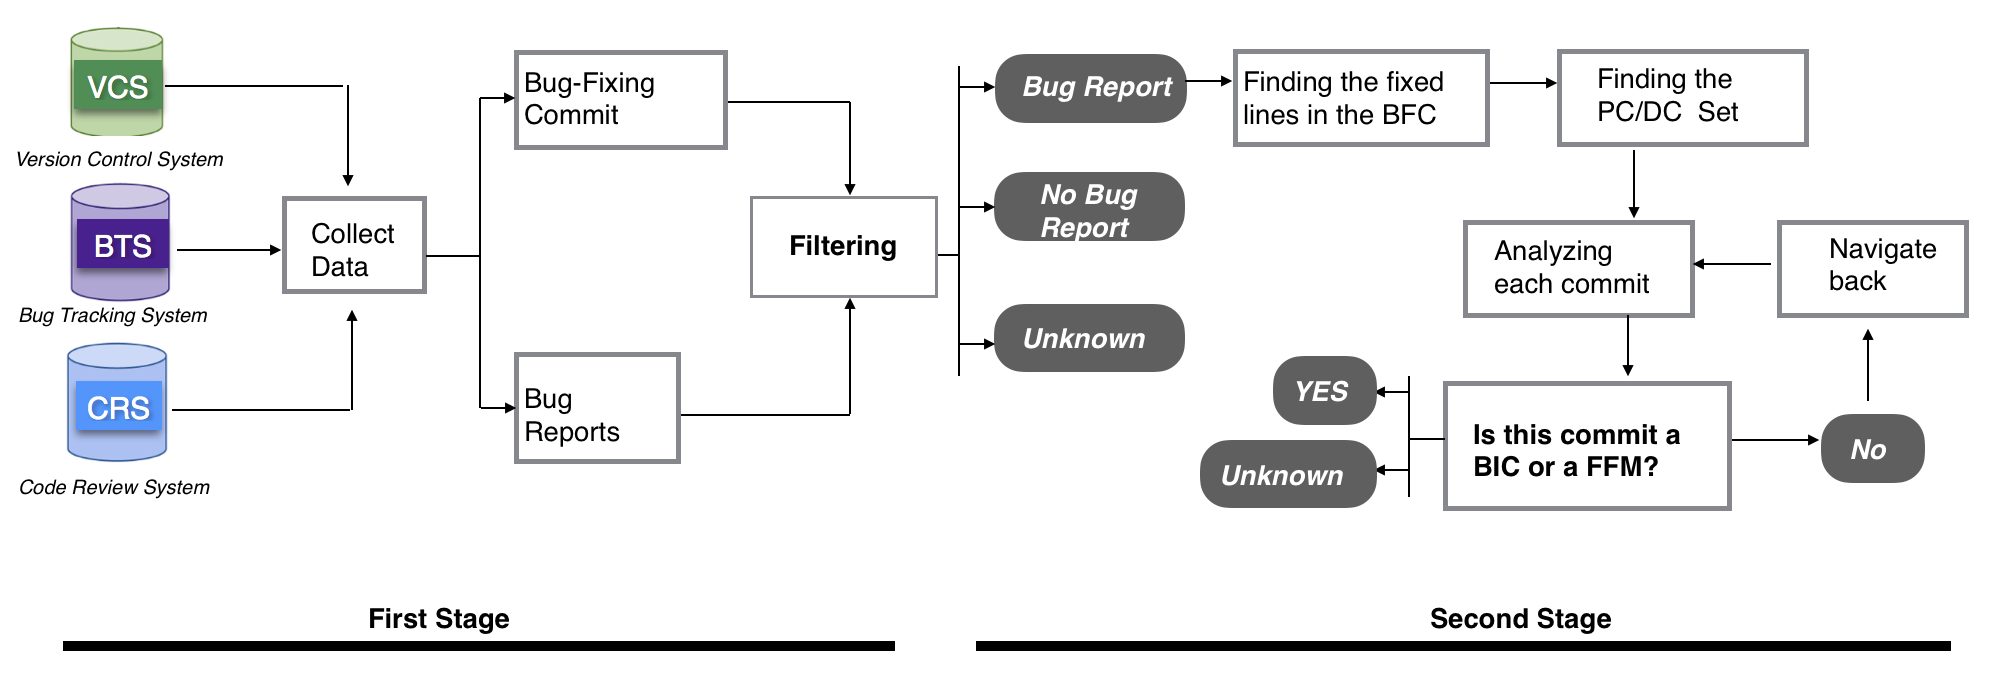
\includegraphics[width=\columnwidth]{img/diagram.png}
 \caption{Overview of the steps involved in our analysis }
 \label{fig:diagram}       % Give a unique label
 \end{figure}

\subsection{Identifying the First Failing Commit and the Bug Introducing Change of a bug report}
To analyze the fixing-commit of a bug report in order to find the Bug Introducing Change, when it exists, and the First Failing Commit. The first author follows next steps in order to identify both commits, when it is possible.

\subsubsection{Finding the lines that fixed the bug}
At this stage, we have to find the source code that fixed a bug $b$. Therefore, we have to:
	\begin{itemize}
		\item Identify the change(s) that fixed the bug,\setBFC{b}\footnote{ The anlayzed \BFC from Nova always fixed a unique bug, but we found a few number of \BFC that fixed more than one bug in ElasticSearch. However, we were able to distinguish which change fixed each bug, and to simplify, we are going to assume in the methodology that in \setBFC{b} only there will be a unique \BFC}
	%	After fixing a bug, it is common practice in many open source projects, that developers provide information in the ticket threat of bug, including a link to the commit in the versioning system.
		\item Find the lines that the \setBFC{b} added, modified or deleted to fix the bug, \LC{c_l} where c\_l is the \BFC:
	All the information related with the code review process can be found in the bug report. By applying \textit{``git diff''} to the files touched by the \BFC we can identify what lines have been added, modified or deleted between the version after the \setBFC{b} and the previous one.
		\item Filter out lines that are not code:
		Lines that have been modified, but do not contain source code (e.g., comments or blank lines) are not considered. Furthermore, we also filter out test files, because when they are touched by the \setBFC{b} they are implementing the test cases for the fixed lines.
	\end{itemize}

\subsubsection{Determining, for each of those lines, \LC{c_l}, what commit changed these lines for the last time}
Each individual line touched by the \BFC has only one immediately previous commit in the lineal vision precedence graph. However, there could potentially be as many previous commits as modified lines in the \BFC in the ancestor tree graph. Thus, taking the ancestor graph as reference,  the result is a set of all previous commits of the bug $b$, \PC{b}.
In the case where the \BFC only added new lines to fix the bug, these lines cannot be tracked back. However, we analyze the surrondings lines to these added lines in orderr to understand whether some of the commits that introduced the surronding lines missed the code that have been added by the \BFC.

\subsubsection{Analyze each of these previous commit to determine the First Failing commit and the Bug Introduction Commit}

This analysis relies on the information available in the description of the bug report, the bug-fixing message and the control version system. After understanding the context of the bug and the changes made by the \BFC, we select the lines of each \pc belonging to the \PC{b} and navigate back into the \ACS of these lines until find the line, if it is applicable, that introduced the bug and the line that manifested by first time the bug. There are four possible scenarios:

\begin{itemize}
	\item $ \BIC = \FFC $, the moment when the bug was inserted is the same that the moment when the bug manifested itself by first time in the project.
	\item $ \BIC \not= \FFC $, the moment when the bug was inserted is not the same that the moment when the bug manifested itself by first time in the project. This happen when (1) There is not a \BIC, or (2) The \BIC is not in the \ACSet{b}.
	\item $ Unknown $, when we do not have enought information to decide whether the line cause the bug or when the complexity of the \BFC is high and we cannot be sure to find the \FFC and \BIC between all ancestor changes.
\end{itemize}


\subsection{Outcomes}
At the end of the process, we may have the following outcomes for each bug report and also for each commit analized:

\subsubsection{Bug Reports}
There are three possible outcomes for each bug report depending on the FFC and the BIC:

\begin{itemize}
	\item We identify the FFC and the BIC of a bug report.
	\item We identify only the FFC because there was not a BIC in the bug report.
	\item We delimit the FFC in a temporary window because we are not sure about when the bug manifest itselft in the code .
	\item We are unsure whether the BIC exits in the bug report.
\end{itemize}

\subsubsection{Commits}

There are four possible outcomes for each commit analyzed:
\begin{itemize}
	\item It is the first failing commit, the commit manifested by first time the bug in the source code.
	\item It is the bug introducing commit, the commit introduced the erroneous line(s) in the source code.
	\item We are not sure about the nature of the commit
	\item Irrelevant for the analysis. %In addition, according to SZZ algorithm this commit is false positive because the algorithm is able to locate it but it is not the cause of the failure.
\end{itemize}


\section{Resultados}
\section{Conclusiones y Trabajo Futuro}

%%%%%%%%%%%%%%%%%%%%%%%%%%%%%%%%%%%%%%%%%%%%%%%%%%%%%%%%%%%%%%%%%%%%%%%%%%%%%%%%
%%%%%%%%%%%%%%%%%%%%%%%%%%%%%%%%%%%%%%%%%%%%%%%%%%%%%%%%%%%%%%%%%%%%%%%%%%%%%%%%
% BIBLIOGRAFIA %
%%%%%%%%%%%%%%%%%%%%%%%%%%%%%%%%%%%%%%%%%%%%%%%%%%%%%%%%%%%%%%%%%%%%%%%%%%%%%%%%

\cleardoublepage

% Las siguientes dos instrucciones es todo lo que necesitas
% para incluir las citas en la memoria
\bibliographystyle{abbrv}
\bibliography{memoria}  % memoria.bib es el nombre del fichero que contiene
% las referencias bibliogr?ficas. Abre ese fichero y mira el formato que tiene,
% que se conoce como BibTeX. Hay muchos sitios que exportan referencias en
% formato BibTeX. Prueba a buscar en http://scholar.google.com por referencias
% y ver?s que lo puedes hacer de manera sencilla.
% M?s informaci?n:
% http://texblog.org/2014/04/22/using-google-scholar-to-download-bibtex-citations/

\end{document}


%that 33% of the bugs intro- duced in a version are not reported till much later (i.e., they are reported in future versions as dormant bugs)
%we find that they are fixed faster (median fix time of 5 days) than non- dormant bugs (median fix time of 8 days), and are fixed by more experienced developers (median commit counts of de- velopers who fix dormant bug is 169% higher).

% What are the root causes of dormant bugs?
%Our prior RQs were primarily quantitative. They helped shed light into the dormant bug phenomena. However, we still do not have a good understanding as to why dormant bugs occur. In this RQ, we use qualitative analysis to un- ravel the root causes of dormant bugs and whether such causes differ from non-dormant bugs. Such in-depth under- standing will assist future researchers in developing tech- niques to help practitioners cope and avoid dormant bugs.

%Approach. We randomly sampled 357 dormant bug issues to reach a confidence level of 95% and a confidence interval of 5% [33](S. Boslaugh and P.A. Watters. Statistics in a Nutshell: A Desktop Quick Reference. In a Nutshell (O’Reilly). O’Reilly Media, 2008.). We also randomly sampled the same number of non-dormant bug issues for comparison. The first author of the paper then manually examined each issue and classified them into one of the root cause categories.
